\PassOptionsToPackage{dvipsnames}{xcolor}    
\documentclass[12pt,letterpaper]{report}
\usepackage{natbib}
\usepackage{geometry}
\usepackage{fancyhdr}
\usepackage{afterpage}
\usepackage{graphicx}
\usepackage{amsmath,amssymb,amsbsy}
\usepackage{dcolumn,array}
\usepackage{tocloft}
\usepackage{asudis}



%%%%%%%%%%%%%%%% PACKAGES ADDED BY TGOKHALE %%%%%%%%%%%%%%%%
% \usepackage[dvipsnames]{xcolor}
\usepackage{epsfig}
\usepackage{graphicx}
\usepackage{amsmath}
\usepackage{amssymb}
\usepackage{amsfonts}
\usepackage{bbm}
\usepackage[normalem]{ulem} 
\usepackage{booktabs}
\usepackage{multirow}
\usepackage{makecell}
\usepackage{enumitem}
\usepackage{epigraph}
\usepackage{mathtools}
\usepackage{textgreek}
\usepackage{color, colortbl}
\usepackage{sepfootnotes}

\definecolor{LightCyan}{rgb}{0.88,1,1}
\definecolor{LightRed}{rgb}{1.0, 0.91, 0.91}
\definecolor{LightGray}{rgb}{0.88,0.88,0.88}
\definecolor{VeryLightGray}{rgb}{0.93,0.93,0.93}
%%%%%%%%%%%%%%%% COMMANDS ADDED BY TGOKHALE %%%%%%%%%%%%%%%%
\renewcommand{\thefootnote}{\fnsymbol{footnote}} 
\newcommand\BibTeX{B\textsc{ib}\TeX}
\renewcommand{\epigraphwidth}{\columnwidth}
% \renewcommand{\epigraphflush}{flushright}
\renewcommand{\textflush}{flushright}
\makeatletter
\newcommand{\printfnsymbol}[1]{%
  \textsuperscript{\@fnsymbol{#1}}%
}

\DeclareMathOperator*{\E}{\mathbb{E}}
\DeclareMathOperator{\R}{\mathbb{R}}
\DeclareMathOperator{\x}{\mathbf{x}}
\DeclareMathOperator{\y}{\mathbf{y}}
\DeclareMathOperator*{\domain}{dom}
\DeclareMathOperator*{\argmax}{argmax}
\DeclareMathOperator*{\union}{\bigcup}
\DeclarePairedDelimiter\floor{\lfloor}{\rfloor}
\newcommand{\textul}{\uline}

\newcommand*\samethanks[1][\value{footnote}]{\footnotemark[#1]}

%%%%%%%%%%%%%%%% PACKAGES ADDED BY TGOKHALE %%%%%%%%%%%%%%%%
% \usepackage[dvipsnames]{xcolor}
\usepackage{epsfig}
\usepackage{graphicx}
\usepackage{amsmath}
\usepackage{amssymb}
\usepackage{amsfonts}
\usepackage{bbm}
\usepackage[normalem]{ulem} 
\usepackage{booktabs}
\usepackage{multirow}
\usepackage{makecell}
\usepackage{enumitem}
\usepackage{epigraph}
\usepackage{mathtools}
\usepackage{textgreek}
\usepackage{color, colortbl}
\usepackage{sepfootnotes}

\definecolor{LightCyan}{rgb}{0.88,1,1}
\definecolor{LightRed}{rgb}{1.0, 0.91, 0.91}
\definecolor{LightGray}{rgb}{0.88,0.88,0.88}
\definecolor{VeryLightGray}{rgb}{0.93,0.93,0.93}
%%%%%%%%%%%%%%%% COMMANDS ADDED BY TGOKHALE %%%%%%%%%%%%%%%%
\renewcommand{\thefootnote}{\fnsymbol{footnote}} 
\newcommand\BibTeX{B\textsc{ib}\TeX}
\renewcommand{\epigraphwidth}{\columnwidth}
% \renewcommand{\epigraphflush}{flushright}
\renewcommand{\textflush}{flushright}
\makeatletter
\newcommand{\printfnsymbol}[1]{%
  \textsuperscript{\@fnsymbol{#1}}%
}

\DeclareMathOperator*{\E}{\mathbb{E}}
\DeclareMathOperator{\R}{\mathbb{R}}
\DeclareMathOperator{\x}{\mathbf{x}}
\DeclareMathOperator{\y}{\mathbf{y}}
\DeclareMathOperator*{\domain}{dom}
\DeclareMathOperator*{\argmax}{argmax}
\DeclareMathOperator*{\union}{\bigcup}
\DeclarePairedDelimiter\floor{\lfloor}{\rfloor}
\newcommand{\textul}{\uline}

\newcommand*\samethanks[1][\value{footnote}]{\footnotemark[#1]}


\DeclareMathOperator{\xx}{\mathrm{x}}
\DeclareMathOperator{\yy}{\mathrm{y}}
\DeclareMathOperator{\zz}{\mathrm{z}}
\DeclareMathOperator{\cc}{\mathrm{c}}
\let\vv\relax
\DeclareMathOperator{\vv}{\mathrm{v}}
\DeclareMathOperator{\uu}{\vec{\mathbf{u}}}
\DeclareMathOperator{\qq}{\mathbf{q}}
\def\vec{\mathaccent "017E\relax }

% \usepackage{skt}
% sanskrit
% \usepackage{fontspec}
% \newfontfamily\hindifont{Noto Sans Devanagari}[Script=Devanagari] % Use any Devanagari font on your system

\usepackage[plainpages=false,pdfpagelabels,bookmarks,bookmarksnumbered,hidelinks]{hyperref}
\hypersetup{
    colorlinks=true,
    linkcolor=Blue,
    citecolor=magenta,
    urlcolor=blue
    }
    
% Support for easy cross-referencing
\usepackage[capitalize]{cleveref}
\crefname{section}{Sec.}{Secs.}
\Crefname{section}{Section}{Sections}
\Crefname{table}{Table}{Tables}
\crefname{table}{Tab.}{Tabs.}

\begin{document}
%-----------------------front matter
\pagenumbering{roman}
\title{Discovering and Designing Transformations for Robust Visual Understanding}
\author{Tejas Gokhale}
\degreeName{Doctor of Philosophy}
\defensemonth{April}
\gradmonth{May}
\gradyear{2023}
\chair{Yezhou Yang, Co-Chair \\ Chitta Baral, Co-Chair \\ Heni Ben Amor\\ Rushil Anirudh}		
\maketitle
\doublespace

\newpage
\vspace*{\fill}
\noindent 
\copyright~~Tejas Gokhale. All Rights Reserved.\\
% Re-distributed by Arizona State University under license from Tejas Gokhale.\\

\begin{wrapfigure}{l}{0.3\linewidth}
    
\includegraphics[width=\linewidth]{figures/cc_by_nc.png}
\end{wrapfigure}
\noindent This work is licensed under a Creative Commons Attribution-Noncommercial 4.0 International License.\\
\url{https://creativecommons.org/licenses/by-nc/4.0/}

\begin{abstract}
The advances in machine learning have brought about impactful improvements in perception, especially in systems that can understand images.
This thesis proposal aims to complement these improvements by studying the robustness and generalization capabilities of vision and language models.
This involves (1) identifying failure modes, i.e., situations under which these systems are prone to fail, (2) creating analysis tools and  evaluation benchmarks and metrics to help detect and diagnose these failures, and (3) developing machine learning algorithms that provide greater robustness and generalization to mitigate the risks posed by such situations.
In particular, this proposal describes five research projects -- two in image classification and three in multi-modal vision-and-language tasks that address the above goals.
AGAT is designed for making image classifiers robust to unknown shifts along pre-specified image attributes, ALT addresses the harder task of single-source domain generalization, VQA-LOL tackles logical compositions in visual question answering, ``Mutant'' is a data augmentation technique for reducing the problem of VQA dataset bias, and SDRO is a new distributed robust optimization method that uses semantic sentence transformations for improving the robustness of vision-language inference models.
Three potential research directions are discussed, (1) an empirical study of comparative effect of dataset modification on out-of-distribution accuracy and adversarial robustness, (2) a hypothesis that analyzing the interpolations between two images might point to insights about image classifier robustness, and (3) designing evaluation protocols for pre-trained V\&L models.
\end{abstract}

\dedicationpage{\\
% oṃ saha nāvavatu .\\
% saha nau bhunaktu .\\
% saha vīryaṃ karavāvahai .\\
% tejasvi nāvadhītamastu mā vidviṣāvahai .\\
% oṃ śāntiḥ śāntiḥ śāntiḥ ..
\vspace*{12pt}
\begin{figure}[h]
    \centering
    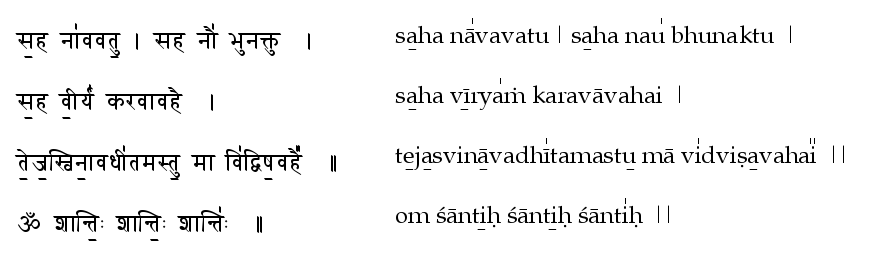
\includegraphics[width=\linewidth]{figures/shanti_mantra.png}
\end{figure}

\hspace*{\fill}{Taittiriya Upanishad 2.1.1.} \\

\begin{flushleft}
Om, may it (Knowledge), protect us both (the teacher and the student).\\
May it nourish us both.\\
May we generate great energy. \\ %work together with great energy.\\
May our study lead to Brilliance (of Understanding, leading to Knowledge).\\
May it not give rise to hostility (due to lack of Understanding).\\
Om, Peace, Peace, Peace.
% \item[] Om, peace (in me), peace (in nature), peace (in divine forces)
\end{flushleft}
}
\acknowledgementpage{\\

{
\begin{FlushRight}
    ``Knowledge is in the end based on acknowledgement.''\\
    - Ludwig Wittgenstein\\
    \medskip
    \hrule 
    \bigskip
\end{FlushRight}
}

\begin{justify}
I would like to express my deepest gratitude to my advisors Yezhou Yang and Chitta Baral, who have been an unconditional source of encouragement, and a crucial support system before, during, and after the pandemic.  Yezhou and Chitta offered a rather delicious blend of advise, offering up combo-style meals of big picture messaging + practical and grounded methods,  vision + language (literally and metaphorically).
% \textit{karma-yog} (the path of action) + \textit{jnana-yog} (the path of knowledge).  
While most of my Ph.D.\ journey was clouded by the pandemic, Yezhou and Chitta offered me their unflinching support and encouragement and helped me navigate myself out of local minima.  They created a healthy work environment that allowed me to explore, stumble, and to learn to pick myself up.  It has been an absolute privilege to learn, collaborate, dream, and disagree with Yezhou and Chitta.


I am also grateful for the mentorship of Rushil Anirudh at Lawrence Livermore National Laboratory.
The terrific trio of Rushil, Jay Thiagarajan, and Bhavya Kailkhura introduced me to many ideas in robustness and generalization, making my two summers ``at'' LLNL a game-changer for my Ph.D.\ thesis. 


Microsoft


I am indebted to the knowledge I received from exemplary \textit{gurus} -- creators and sustainers of knowledge and destroyers of ignorance.
I have been fortunate to have learned Machine Learning from Nina Balcan and Gautam Dasarathy, Deep Learning from Ruslan Salakhudtinov, Convex Optimization from Aarti Singh, Computer Vision from Deva Ramanan and Suren Jayasuriya, Speech and Natural Language Processing from Alan Black, and a re-education in signal processing from Aswin Sankaranarayanan. 
I would like to thank Aswin for advising me at Carnegie Mellon University and and Kuldeep Kulkarni who mentored my first research project of substance.
Aswin introduced me to the art of research and was the catalyst in my decision to pursue a Ph.D.
Kuldeep's knack of turning whiteboard sketches (or chess-board enactments) into concrete research ideas was inspirational.


And then are the unsung heroes of ASU -- Pamela Dunn and Monica Dugan in the SCAI Business Office, Jaya Krishnamurthy and Arzuhan Kavak in SCAI Advising, Theresa Chai in SCAI Finance, Lincoln Slade and Brint MacMillan in SCAI IT, Katrina Roalson and Pamela Felix in ASU Graduate College, Sydney Burt in GPSA, and ASU ISSC for their priceless support in navigating logistics, computing and infrastructure, administrative issues, conference travel, fellowships and payroll.


I also owe much to my wonderful collaborators at ASU -- Pratyay Banerjee, Zhiyuan Fang, Man Luo, Swaroop Mishra, Neeraj Varshney, Joshua Feinglass, Ethan Wisdom, Sheng Cheng and my talented mentees Abhishek Chaudhary, Huiliang Shao, Maitreya Patel, and Agneet Chatterjee who kept me on my toes.
I would also like to thank my friends Lu Cheng, Kowshik Thopalli, John Janiczek, Mohammad Farhadi, Changhoon Kim, Varun Jammula, Rudra Saha, Sam Rawal, Aurgho Bhattacharjee, Ishan Shrivastava, Kuntal Pal, Mihir Parmar, Raha Moraffah, Kaize Ding, and all members of the APG, CogInt, and Summer Vision Reading Groups.
I am also thankful for the \textit{TFG++}, whom I consider to be family.
I would like to mention my appreciation for my bookshelf which has grown to insane proportions;
% but has been often (and unfortunately) ignored and replaced by Netflix, and YouTube. It 
it continues to aid and abet my pretension of being a well-read intellectual.


I am extremely fortunate and privileged to have grown up in an atmosphere of love, care, integrity, and excellence, created by my parents Ravindra Gokhale and Mugdha Gokhale who made me who I am today, and my sister Meghana for leading by example.
I am thankful to my grandparents Dr.\ Manohar Joshi and Dr.\ Sulekha Joshi who introduced me to the romance and joy of learning.
Finally, I am thankful to generations of courageous Bharatiyas who liberated my motherland from 1000 long years of terrorism, subjugation, and colonization; without their sacrifices, I would not have had the opportunity of being who I am today.
\end{justify}
}
\tableofcontents
% This puts the word "Page" right justified above everything else.
\addtocontents{toc}{~\hfill Page\par}
% Asking LaTeX for a new page here guarantees that the LOF is on a separate page
% after the TOC ends.
\newpage
% Making the LOT and LOF "parts" rather than chapters gets them indented at
% level -1 according to the chart: top of page 4 of the document at
% ftp://tug.ctan.org/pub/tex-archive/macros/latex/contrib/tocloft/tocloft.pdf
\addcontentsline{toc}{part}{LIST OF TABLES}
\renewcommand{\cftlabel}{Table}
\listoftables
% This gets the headers for the LOT right on the first page.  Subsequent pages
% are handled by the fancyhdr code in the asudis.sty file.
\addtocontents{lot}{Table~\hfill Page \par}
\newpage
\addcontentsline{toc}{part}{LIST OF FIGURES}
\addtocontents{toc}{CHAPTER \par}
\renewcommand{\cftlabel}{Figure}
% This gets the headers for the LOF right on the first page.  Subsequent pages
% are handled by the fancyhdr code in the asudis.sty file.
\addtocontents{lof}{Figure~\hfill Page \par}
\listoffigures
%-----------------------body
\doublespace
\pagenumbering{arabic}
\chapter{Introduction}
\label{chap:introduction}
Humans, from time immemorial, have looked at the earth and seen things interacting with each other; they have looked at the skies and wondered what the stars and planets were; they have looked at each other and invented communication, co-operation, society, and culture.
The process of observing the world and understanding these observations is arguably still the way we reason about the world.
Ever since the democratization of cameras, the process of reasoning about visual observations has become computational.
% Camera technology has made that process of reasoning about wa computational one.
The pursuit of developing such computations \textit{is} computer vision.
When the outputs of the reasoning process convey meaningful concepts to humans, we shall call it semantic visual understanding.

This introductory chapter is designed to be a bird's-eye-view of semantic visual understanding.
First, I will introduce a hierarchy of computer vision tasks that allows us to separate semantics from physics.
Second, I will briefly revisit the progress made in prototypical computer vision tasks and the benchmarks and datasets that have been established by researchers over the years for these tasks.
Third, we will discuss the implications of recent successes in computer vision and motivate the core ideas of this thesis along with an outline.
This will lay the groundwork for the rest of this dissertation.
Chapter \ref{chap:background} is meant to be a technical treatment of the background, related work, and existing methodologies for robust visual understanding.

\section{Understanding What Cameras See} 
\begin{figure}[t]
    \centering
    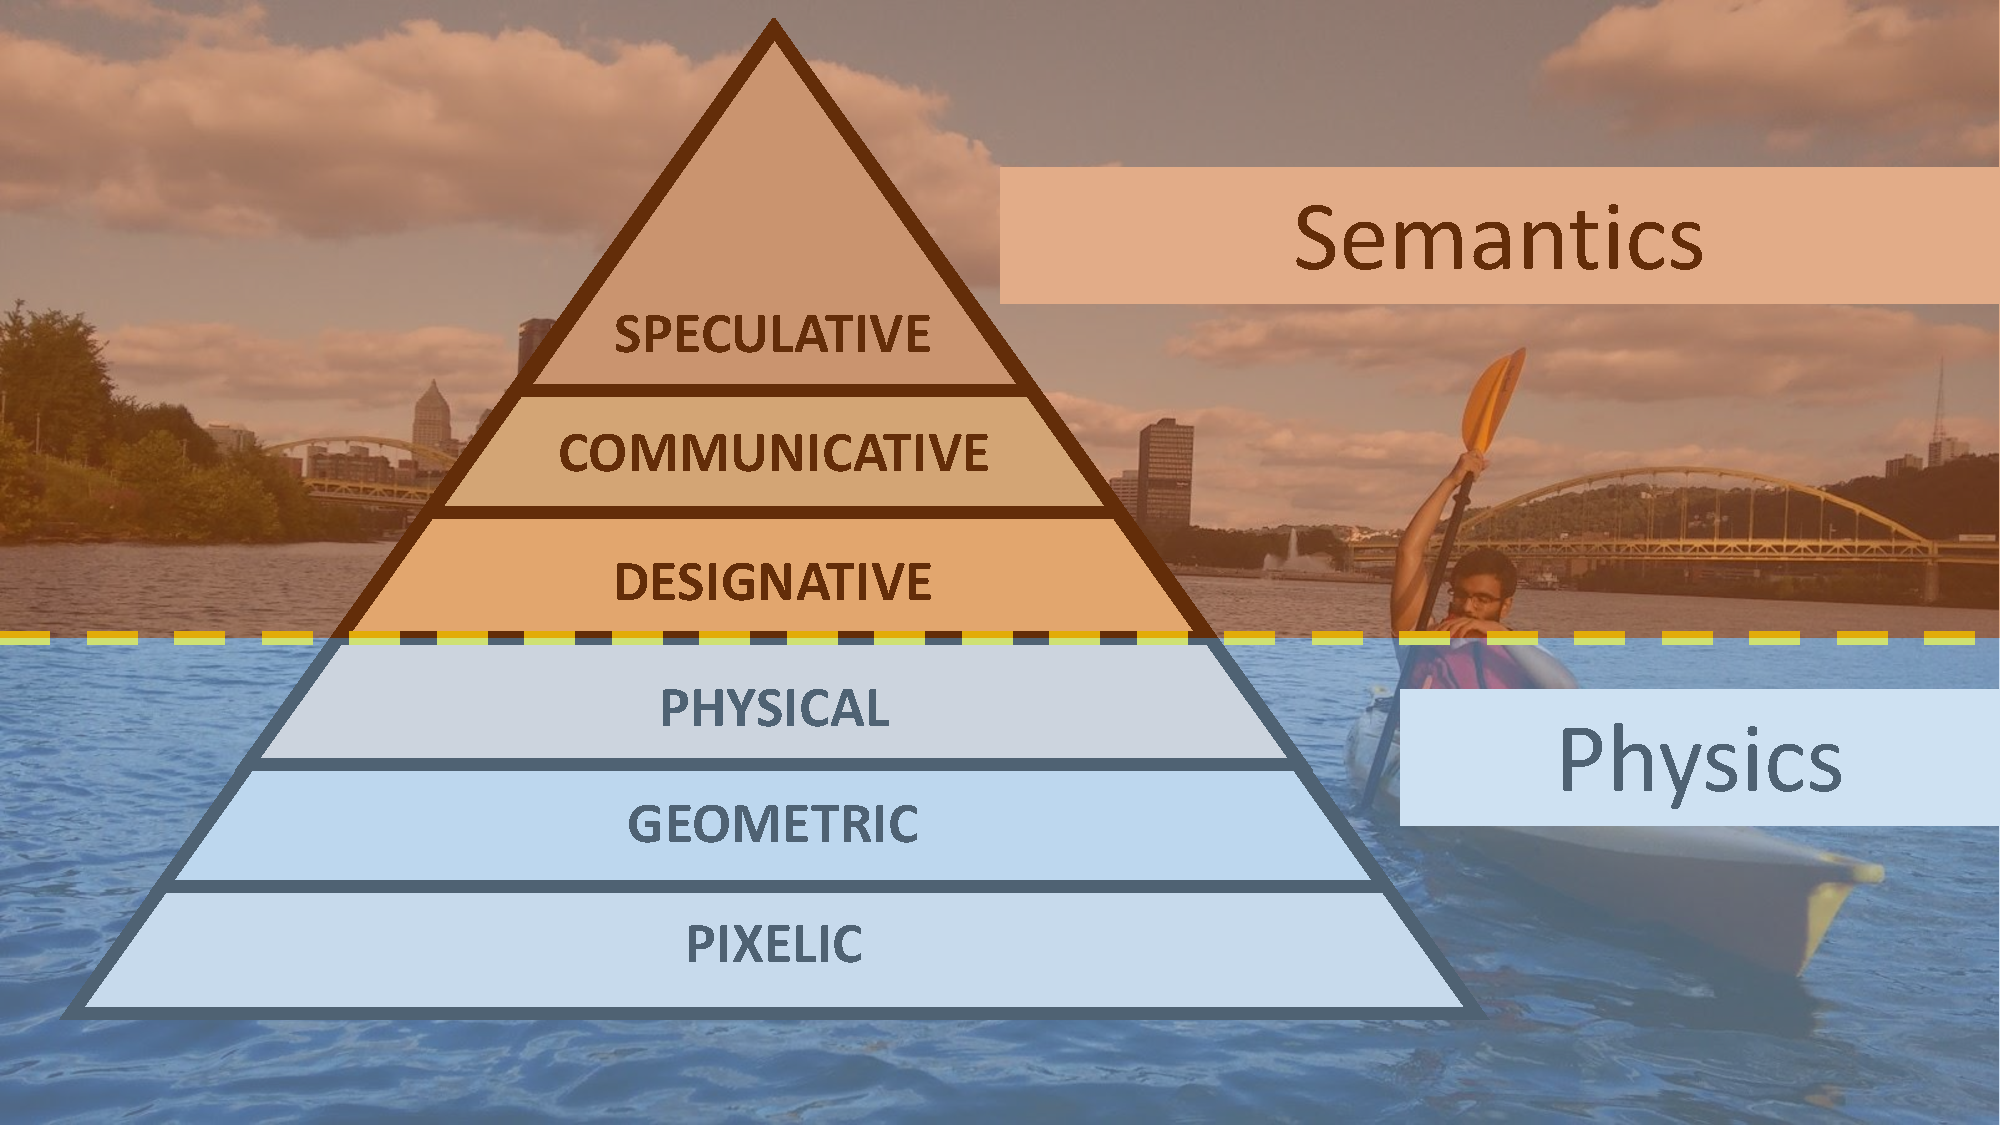
\includegraphics[width=\linewidth]{figures/visual_understanding_pyramid.pdf}
    \caption{A pyramidal hierarchy of visual understanding. This thesis largely deals with semantic vision, especially designative and communicative aspects of semantic vision.}
    \label{fig:visual_understanding_pyramid}
\end{figure}
While computer vision traces its roots and shares many of the goals of digital image processing~\citep{rosenfeld1976digital}, in the 1970s, computer vision underwent a paradigm shift.
While image processing was more focused on developing algorithms for acquisition, storage and information extraction from images, computer vision researchers are motivated by a larger goal -- to \textit{recover} information about scenes that is lost when an image is captured by a camera.
This includes \textit{``pixelic''} analysis such as edge detection and color detection; \textit{``geometric''} properties of the scene, for instance, three-dimensional properties such as depth, surface normals, orientation, and shape; and \textit{``physical''} properties of the scene such as estimating material reflectances, albedo, texture, etc. 
Computer vision also seeks to understand what objects (such as people, boats, trees, bridges, buildings) are present in an image, and where (localization). I call this category of vision, \textit{``designative''} vision since the aim is to designate or assign names and categorical labels to the observed visual input.
More recently, computer vision has also begun to serve in a \textit{``communicative''} role, for instance, the task of learning captions for images~\citep{yang2011corpus,karpathy2015deep} allows computer vision algorithms to express the scene in a human-understandable format.
Similarly, visual question answering~\citep{antol2015vqa} enable users to ask questions about the image and get answers from the computer vision system.
There has also been interest in \textit{``speculative''} vision, sometimes also controversially referred to as ``commonsense''~\citep{zellers2019recognition,park2020visualcomet} in literature; the aim is to speculate about intentions of people, their relationship with each other or with other objects, to speculate about their past or future actions and the effect of these actions, or to reason about why those actions are being performed.

Figure~\ref{fig:visual_understanding_pyramid} summarizes this hierarchy of visual understanding into six broad categories, and divides this spectrum into two main parts -- semantic vision and physics-based vision.
\textit{This thesis focuses on semantic vision.}


\section{Recent Success In Visual Understanding}
The fabled memo-meme from the 1950s to ``solve'' computer vision as a summer project ~\citep{papert1966summer} has grown as one of the biggest and most active research programs of scientific research in recent years~\citep{su2021affective}.
Computer vision occupies a large role in the popularity and applicability of machine learning algorithms.
Several standards benchmarks have been established, adopted, and celebrated by the community for many vision tasks.
Below, I will briefly review progress made on some of these datasets which lie in the category of \textit{``designative''} and \textit{``communicative''} vision tasks such as image classification, object detection, semantic segmentation, image captioning, and visual question answering.
\begin{description}
    \item \textbf{Image Classification.}
    \textit{MNIST}~\citep{lecun1998mnist}, introduced in 1998, is a handwritten digit classification; the efficacy of the convolutional neural network architecture and learning via backpropagation~\citep{lecun1989backpropagation} was demonstrated on MNIST.
    Today, machine learning systems are used by many businesses including the US Post Office, to flawlessly convert handwritten digits, into digital formats.
    \textit{ImageNet}~\citep{deng2009imagenet}, introduced in 2009, proved to be a catalyst for the emergence of neural networks as the de-facto solution for many problems in perception.
    % Convolutional neural networks were shown to be highly effective classifiers and achieved human-level performance on the ImageNet benchmark.
    % While traditional approaches based on SIFT~\citep{lowe2004distinctive,sanchez2011high} had reached a top-5 accuracy of $74.3\%$ in 2011, q
    Quick progress was made via 
    % convolutional neural networks such as 
    AlexNet~\citep{krizhevsky2012imagenet} and 
    % demonstrated a $83\%$ top-5 accuracy, and within three years,three years, 
    ResNet~\citep{he2016deep} reached $96.4\%$ on the same metric.
    ResNet features, i.e. the features of a ResNet model pretrained on ImageNet, became a standard choice for initialization of neural networks.
    In 2021, the top-5 accuracy is ${\sim}99\%$\footnote{performance metrics obtained from \url{https://paperswithcode.com/sota/}}.
    \textit{CIFAR-10 and CIFAR-100}~\citep{krizhevsky2009learning} were introduced in 2009; at that time, RBM-based methods~\citep{} achieved ${\sim}60\%$ accuracy on CIFAR-10, while in 2021, the Vision Transformer~\citep{} reports an accuracy of $99.50\%$.
\item \textbf{Object Detection.}
    \textit{PASCAL-VOC}~\citep{everingham2010pascal} (2010) and \textit{MS-COCO}~\citep{lin2014microsoft} (2014) are popular benchmarks for the task of object detection -- predicting the categories and locations of multiple objects in an image.
    While traditional approaches based on deformable parts model~\citep{fidler2013bottom} had reached a mean average precision of ${\sim}40\%$ and $29.6\%$ on PASCAL-VOC and $19.1\%$ on MS-COCO in 2014, in 2021, neural network object detectors report $62.4\%$ and $89.30\%$ on the same metric.
\item \textbf{Semantic Segmentation.}
ADE20K~\citep{zhou2017scene} and Cityscapes~\citep{cordts2016cityscapes} introduced in 2017 and 2016 respectively are popular benchmarks for semantic segmentation -- the task of assigning a categorical label for each pixel in the image.
Performance on ADE20K has improved from a mean-IoU of $44.94$ in 2017 to $59.90$ in 2021, and performance on Cityscapes has improved from $73.60$ in 2017 to $84.40$ in 2021.
\item \textbf{Image Captioning}.
    \textit{MS-COCO}~\citep{lin2014microsoft} and \textit{Flickr-30k}~\citep{young-etal-2014-image}, both introduced in 2014 are popular benchmarks for the task of image captioning, i.e. generating a natural language description for an input image.
    In 2015, the performance in terms of BLEU-4 score~\citep{papineni2002bleu} was $23.0$ and $15.7$ respectively, while in 2021, this has increased to $37.4$~\citep{li2020oscar} and $30.10$~\citep{zhou2020unified}, respectively.
\item \textbf{Visual Question Answering.}
Several datasets based on images from MS-COCO, VisualGenome, etc. have been used for visual question answering, i.e., predicting answers for questions about an image.
VQA-v2~\citep{goyal2017making} is a popular benchmark for this task, with accuracy improving from $62.7\%$ in 2016~\citep{fukui2016multimodal} to ${\sim}80\%$ in 2021~\citep{zhang2021vinvl,li2020oscar}.
\end{description}
% \item \textit{Visual Reasoning} 

% \item[Image Generation]
%     using neural networks was made sophisticated after the introduction of Generative Adversarial Networks (GANs)~\citep{goodfellow2014generative} which were able to produce remarkably photorealistic images from noise.
%     Since then significant advances have been made in this domain, to such an extent, that DeepFakes (i.e. images and videos manipulated or synthesized by algorithms) have been discussed in the United States Congress~\footnote{\url{https://www.youtube.com/watch?v=lArPEDS0GTA}} as a national security threat.
% \item[Vision+Language] has emerged as a new and exciting area of machine learning as it builds on advances made in two domains: computer vision and natural language processing.
% {\color{red}
% basically in this first paragraph, just quickly review some of the most impactful methods that have sparked tremendous progress (convolutional networks, LSTMs and transformers -- quickly report their performance on highly popular benchmarks in vision and NLP).
% - recent successes in vision, in NLP, and in semantic vision (start with ``a new paradigm of visual understanding has emerged that interacts with natural language -- I call it semantic visual understanding -- this can be either by taking the aid of language to understand vision better, or to express visual understanding in terms of natural language'').

% then introduce multi-modal methods like bottom-up up to OSCAR, report performance on V\&L tasks

% here pivot to the need for robust visual understanding being more crucial/critical/imminent than ever before

% }

\section{What Does Success on a Benchmark Imply?}
These results clearly indicate the semantic vision has seen substantial improvements over the last decade.
This progress, powered largely by innovations in neural network architectures, optimization techniques, and availability of copious amounts of training data, is definitely good news.
These results corroborate prior theoretical work on learnability in statistics and machine learning~\citep{valiant1984theory,hoeffding1994probability,hornik1989multilayer}.
% ``clearly, while architectures and learning methodologies have caught up spectacularly with theory about learnability in statistical ML (like Hoeffding / universal approximation etc.), we have not even begun to understand when, how, and why models fail under certain unseen situations.
% talk emphatically like this for a few sentences to motivate this thesis.
% thanks largely to the availability of large datasets, and the exceptional effectiveness of neural-network based modeling techniques in fitting non-convex and higher order functions to the data.
% If semantic vision has indeed reached (or surpassed human-level abilities) according to the above results, are we done?
% Are we done? 
Does the performance on standard metrics and benchmarks mean that the problem of \textit{understanding what cameras see} is close to being ``solved''?
Has semantic vision has indeed reached (or surpassed human-level abilities) according to the above results, as some news articles claim?

\begin{figure}
    \centering
    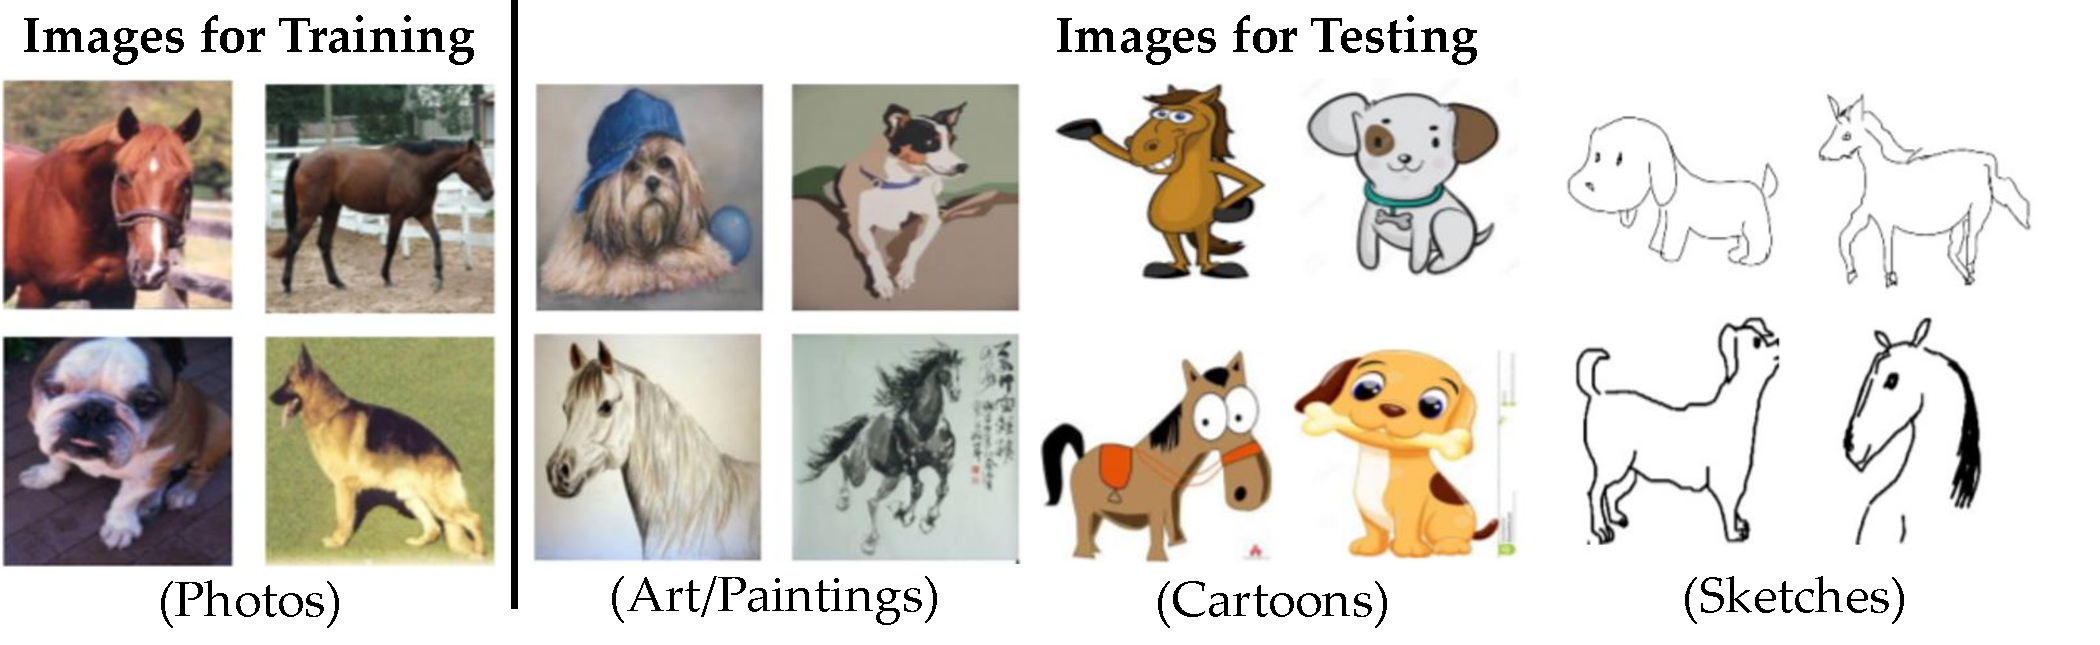
\includegraphics[width=\linewidth]{figures/pacs_styles.pdf}
    \caption{Illustration of the discrepancies between training data and real-world test data. A \textit{robust} image classifier is expected to perform reliably on a wide range of image styles and sources.
    Image adapted from \citet{li2017deeper}.
    }
    \label{fig:pacs_styles_introduction}
\end{figure}

\begin{figure}
    \centering
    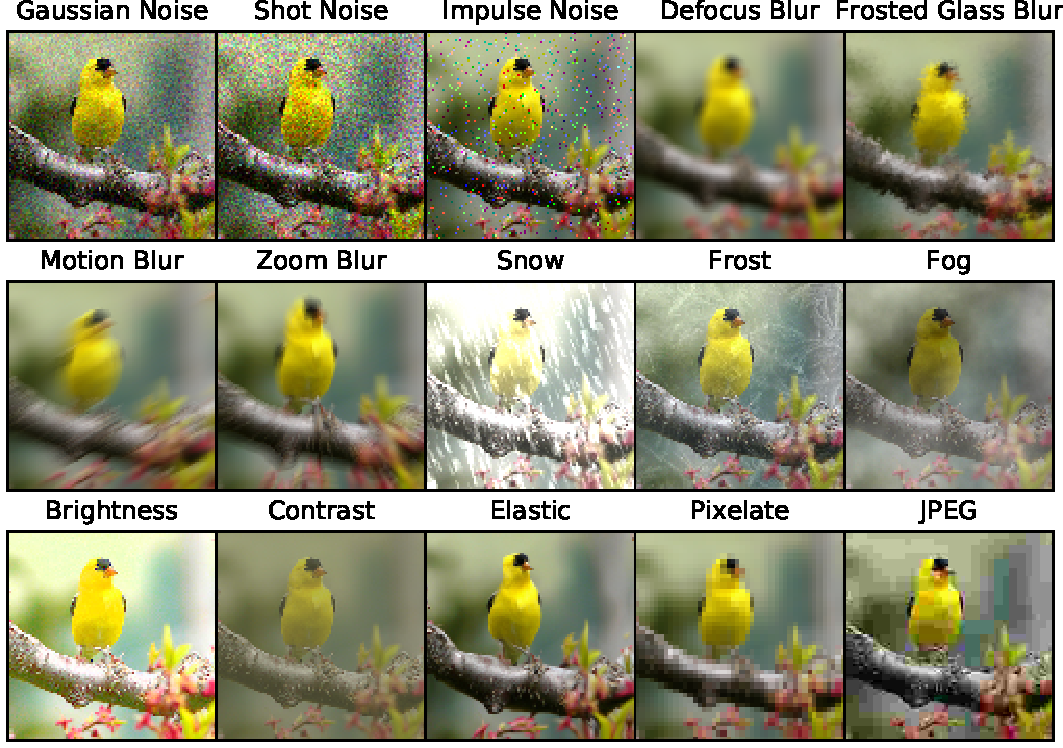
\includegraphics[width=\linewidth]{figures/distorted.pdf}
    \caption{
    Noise, blur, weather, or digital artifacts can also impact classifier performance at test-time.
    Image from \citet{hendrycks2018benchmarking}.
    }
    \label{fig:cifar_c_introduction}
\end{figure}
The answer to these questions, unfortunately is in the negative.
Although highly capable of learning from training data, recent studies show that neural networks are prone to failure on new test sets or under distribution shift~\citep{taori2020measuring}, natural corruptions~\citep{hendrycks2018benchmarking}, adversarial attacks~\citep{goodfellow2014explaining}, spurious correlations~\citep{beery2018recognition}, and many other types of ``unseen'' changes in test samples.
This shortcoming stems from the \textit{i.i.d.} assumption in statistical machine learning which guarantees good performance only on test samples that are drawn from an underlying distribution that is identical to the training dataset.

Consider the case of digit classification.
Digit recognition models trained on the black-and-white MNIST training images are almost perfect ($>99.5\%$ accuracy) on the corresponding \textit{i.i.d.} test set, yet their performance on colored digits and real-world digits from street number plates is only around $70\%$~\citep{xu2020robust}.
Although the accuracy of image classifiers on multiple datasets of real-world photographs such as ImageNet and CIFAR is above $90\%$, when these models are used for classifying other styles of images (such as cartoons, sketches, paintings, etc.)~\citep{venkateswara2017deep,li2017deeper} belonging to the same classes, a performance degradation is observed -- the accuracies are as low as $24\%$ for cartoons, $29\%$ for sketches, $64\%$ for paintings~\citep{nam2021reducing}, as shown in Figure~\ref{fig:pacs_styles_introduction}
There is also a large accuracy drop when models are tested on natural corruptions~\citep{hendrycks2018benchmarking} such as fog, snow, rain, noise, blur etc. or geometric perturbations such as rotation, translation, scaling~\citep{wong2020learning}, as illustrated in Figure~\ref{fig:cifar_c_introduction}.
In short, when models that have been trained in ``lab settings'' are tested in ``real-world settings'', the levee breaks, and we start getting a glimpse into the robustness of computer vision models. 
\textit{This thesis is about identifying such modes of failure, analyzing them, and providing solutions for improving model robustness.}

\section{Overview: Towards Robust Visual Understanding}
The recent findings about the brittleness and high sensitivity of models on real-world data pose a significant challenge to the practical adoption of computer vision models and their reliability in the real-world, especially when dealing with sensitive data such as biomedical and satellite imagery, personal information, private records, etc.
In this dissertation, I will address these shortcomings in the domains of image classification as well as multi-modal visual understanding \textit{a.k.a.} vision-and-language (V\&L).
My work complements the new innovations of the past decade, by studying their robustness and generalization capabilities.
This involves:
\begin{enumerate} 
    \item \textbf{identifying failure modes}, i.e., situations under which systems may fail, for perceptual tasks (such as image classification) and semantic tasks (such as visual question answering, visual reasoning, and image/video captioning),
    \item creating \textbf{evaluation and analysis tools} to diagnose failures, achieved by creating datasets for targeted evaluation, probing models with specific types of input perturbations, evaluating generalization under domain shift or across datasets, etc.
    \item \textbf{developing techniques} that provide greater robustness to mitigate the risks posed by such situations.
\end{enumerate}



%%%% AGAT %%%%
In Chapter~\ref{chap:agat}, we consider a setup where robustness is expected over an unseen test domain that is not i.i.d.\ but deviates from the training domain.
While this deviation may not be exactly known, its broad characterization is specified \textit{a} priori, in terms of attributes.
We propose an adversarial training approach which learns to generate new samples so as to maximize exposure of the classifier to the attributes-space, without having access to the data from the test domain.
Our approach enables deep neural networks to be robust against a wide range of naturally occurring perturbations.
We demonstrate the usefulness of the proposed approach by showing the robustness gains of deep neural networks trained using our adversarial training on MNIST, CIFAR-10, and a new variant of the CLEVR dataset.
This work was published as a conference paper in AAAI 2021~\citep{gokhale2021attribute}.

To be successful in single source domain generalization, maximizing diversity of synthesized domains has emerged as one of the most effective strategies. Many of the recent successes have come from methods that pre-specify the types of diversity a model is exposed to during training so that it can ultimately generalize well to new domains. However, na\"ive diversity based augmentations do not work effectively for domain generalization either because they cannot model large semantic shifts, or the span of transforms that are pre-specified, do not cover the semantic shifts commonly occurring in domain generalization. 
%
%
%
%

%%%% ALT %%%%
To address this issue, in Chapter~\ref{chap:alt}, we present a novel framework that uses adversarially learned transformations (ALT) using a neural network to model plausible, yet hard image transformations that fool the classifier. This network is randomly initialized for each batch and trained for a fixed number of steps to maximize classification error. 
With extensive empirical analysis, we find that this new form of adversarial transformations achieve both objectives of diversity and hardness together, outperforming all existing techniques on competitive benchmarks for single source domain generalization. 
We also show that ALT can naturally work with existing diversity modules to produce highly distinct, and large transformations of the source domain leading to state-of-the-art performance.
This work is currently under review at CVPR 2022.
%
%
%
%

%%%% VQALOL %%%%
In Chapter~\ref{chap:vqalol} we start our foray into multi-modal vision-and-language tasks.
Multi-modal tasks involving both vision and language (V\&L) inputs, such as visual question answering (VQA), open up many more types of domain discrepancies that can affect model performance of test time.
For the VQA task, given an image and a question about it, models are trained to predict the answers to those questions.
In VQA-LOL, we discovered that existing VQA models fail when logical transformations such as negation, conjunction, and disjunction are introduced in the questions.
This surprising finding led us to develop a data augmentation tool that allows us to produce logical combinations of multiple questions in the source dataset, and a training objective that is based on Frechet inequalities to guide the predicted probabilities of answers to questions with negation, conjunction, and disjunction.
Thus, given a known transformation between source and target domains, we developed a method that can leverage data augmentation for improving robustness of VQA models.
This work was published as a conference paper in ECCV 2020~\citep{gokhale2020vqa}.
%
%
%
%

%%%% MUTANT %%%%
The work on VQA-LOL spawned off two additional projects: the first, VQA-MUTANT is about a data augmentation strategy to address changing priors between train and test datasets.
In this paper, we make use of simple image transformations which remove objects or change their colors, in addition to the logical transformations developed above. Empirical results  on the VQA-CP challenge~\citep{agrawal2018don} show that this method achieves robustness under changing question-answer priors (i.e.~when the conditional probability of answers given a question type varies between train and test domains).
This work was published as a conference paper in EMNLP 2020~\citep{gokhale2020mutant}.
%
%
%
%

%%% SDRO %%%%
The problem of logical and linguistic brittleness is not limited to VQA.
In Chapter~\ref{chap:sdro}, we consider the task of vision-and-language inference (VLI), i.e. predicting whether an input sentence is \texttt{True} or \texttt{False} for a given image or video.
We define a set of linguistic transformations called ``SISP'' that contain semantics-inverting as well as semantics-preserving text transformations, such as negation, synonyms, antonyms, paraphrasing.
Analysis of VLI models using SISP transformations reveals their brittleness, especially under semantics-inverting phenomena.
While data augmentation techniques have been designed to mitigate against these failure modes, methods that can integrate this knowledge into the training pipeline remain under-explored.
We present \textbf{SDRO},
% \footnote{Code and data will be released upon publication.}
% % \footnote{\href{https://github.com/ASU-APG/VLI_SDRO}{\footnotesize\url{https://github.com/ASU-APG/VLI_SDRO}}}, 
a model-agnostic method that utilizes a set linguistic transformations in a distributed robust optimization setting, along with an ensembling technique to leverage these transformations during inference.
SDRO also allows us to learn in low-resource settings, serving as a smart data augmentation tool -- SDRO models trained only with $80\%$ of the original dataset outperform existing state-of-the-art which utilizes the entire dataset.
This work is currently under review at ACL 2022, and is available as a preprint~\citep{gokhale2021semantically}.
Shortly after, Neeraj Varshney led a project that constructed a larger set of transformations for unsupervised learning for the text-only task of natural language inference. I am third author for this paper, which is currently under review and available as a preprint~\citep{varshney2021unsupervised}.

% Chapter~\ref{sec:collabs} is a compendium of robustness and generalization study done as part of collaboration with Pratyay Banerjee who was the first author for these papers.
% While Pratyay has discussed these ideas on weak supervision from synthetic data and self-supervised training at length in his thesis, in this chapter, I will briefly discuss how model robustness in visual question answering is affected when trained with weak supervision.


\vspace*{\fill}
\paragraph{Disclosure of Funding Sources.}
Work done at ASU has been funded through grants from
National Science Foundation (grants \#1816039, \#1750082, 
Defence Advanced Research Projects Agency (SAIL-ON program \#W911NF2020006, KAIROS program ), 
and Office of Naval Research Research grant \#00014-20-1-2332.
My work as an intern at Lawrence Livermore National Laboratory was performed under the auspices of the U.S. Department of Energy under contract DE-AC52-07NA27344.
The views and opinions of the authors expressed herein do not necessarily state or reflect those of the funding agencies and employers.

% Deep neural networks have emerged as a widely popular architectural choice for modeling tasks in multiple domains such as (but not limited to) computer vision~\citep{yuille2021deep} and natural language processing~\citep{hochreiter1997long,vaswani2017attention}.
% Although highly capable of learning from training data, recent studies show that neural networks are prone to failure on new test sets or under distribution shift~\citep{taori2020measuring}, natural corruptions~\citep{hendrycks2018benchmarking}, adversarial attacks~\citep{goodfellow2014explaining}, spurious correlations~\citep{beery2018recognition}, and many other types of ``unseen'' changes in test samples.
% This shortcoming stems from the \textit{i.i.d.} assumption in statistical machine learning which guarantees good performance only on test samples that are drawn from an underlying distribution that is identical to the training dataset.
% For instance, digit recognition models trained on the black-and-white MNIST training images are almost perfect ($>99.5\%$ accuracy) on the corresponding \textit{i.i.d.} test set, yet their performance on colored digits and real-world digits from street number plates is only around $70\%$.
% Similarly, state-of-the-art NLP models have been shown to fail when negation is introduced in the input~\citep{kassner2020negated}.
% These findings pose a significant challenge to the practical adoption of computer vision models and their reliability in the real-world, especially when dealing with sensitive data such as biomedical and satellite imagery or other mission-critical applications in space exploration or drug discovery.

% My work addresses these shortcomings in the domain of 
% \begin{enumerate}[label=(\textbf{\Roman*}),nosep,noitemsep] % (a), (b), (c), ...
%     \item image classification, and 
%     \item multi-modal tasks (vision+language).
% \end{enumerate}
% The focus of my thesis is to identify the various situations under which machine learning models may fail while making predictions for tasks (\textbf{I}) or (\textbf{II}), and to develop machine learning techniques to mitigate risks posed therein.
% These can be categorized as:
% \begin{enumerate}[label=(\textbf{\Alph*}),nosep,noitemsep]
%     \item domain shift -- i.e.~when the training domain $\mathcal{D}$ and target test domain $\mathcal{D}^\prime$ are not identical -- for instance, a trainind domain with black-and-white digits, and target domain with real-world colored digits.
%     \item local perturbations -- i.e.~situations in which small perturbations such as noise and corruptions are encountered in the inputs at test time.
% \end{enumerate} 
% The choice of solution for \textbf{(A)} depends on how much information about the target domain is available during training.
% In cases when labeled target datasets are available, the best bet would be to include such labeled input-output pairs in the training dataset.
% When unlabeled target samples are available, solutions fall under the umbrella term of \textit{domain adaptation}, and seek to utilize unlabeled images to learn an invariant feature space.
% However when no explicit samples (either labeled or unlabeled) are available, the problem becomes that of \textit{domain generalization}.
% When only a single source of training data is available, this is a very challenging problem because of the limited information available to train the model with just a single source.


\chapter{Background}
\label{chap:background}
Engineered systems often come with conditions for operation -- televisions and phones are rated for use only in a range of temperature values, and voltage standards, beyond which they can malfunction.
Machine learning models are no different -- they operate under a set of assumptions about the inputs.
These assumptions are critical when machine learning models encounter variations in inputs at test time or during deployment.
This chapter contains an overview of existing techniques that have been designed to overcome challenges in machine learning that are encountered as a result of deviations between training and test distributions.
In this chapter, we will review literature on robust machine learning, and relevant work in image classification and visual question answering, which will serve as a starting point for subsequent chapters.

\section{Robust Machine Learning}

\subsection{What is Robustness?}
Robustness is an overloaded word in machine learning and is often used with inconsistent connotations by different researchers.
Before we get into the math, it makes sense to develop a simple intuitive definition that we will stick with in this dissertation.
This simple definition is as follows:  machine learning models are trained on a certain dataset but may encounter different types of changes at test time and with varying degrees -- a robust machine learning model is able to reliably produce outputs irrespective of such changes in inputs.
When these changes are designed (either by humans or by algorithms) to fool the model into making incorrect predictions, we will denote such inputs as adversarial examples; the property of a model which is robust under such circumstances will be denoted as \textit{``adversarial robustness''}.
When the entire input distribution shifts in meaningful ways (for instance, grayscale images vs.~color images, or photos vs.~sketches), we will denote this as domain shift, and the property of models that are robust to such shifts as \textit{``domain generalization''.}



Consider a training distribution $P_{tr}$ consisting of inputs $\x$ and labels $\y$.
Under the empirical risk minimization (ERM), the following risk is minimized:
\begin{equation}
    \mathcal{R}_{ERM} = \E_{(\x, \y) \sim P_{tr}}  ~\ell(f(\x; \theta), \y).
    \label{eq:erm}
\end{equation}
ERM provides generalization guarantees~\citep{vapnik1991principles} for i.i.d.\ test samples, but not for out-of-distribution or adversarial examples~\citep{biggio2013evasion,szegedy2014intriguing}. 

\paragraph{Distributed Robust Optimization (DRO)}~\citep{pmlr-v80-hu18a,sagawa2020distributionally} searches for loss-maximizing perturbations of the input within an $\epsilon$-divergence ball around $P_{tr}$ and minimize the risk over such perturbed distributions.
\begin{equation}
    \mathcal{R}_{DRO}=\underset{P:D(P, P_{tr})<\epsilon}{sup}\E_{(\x, \y) \sim P} \ell(f(\x; \theta), \y).
    \label{eq:std_adv}
\end{equation}
The solution to Equation~\ref{eq:std_adv} guarantees robustness inside such $\epsilon$-bounded distributions $P$.
The inner maximization is typically solved using gradient-based methods~\citep{madry2018towards} over additive perturbations $\delta$ such that $\x+\delta$ fools the classifier.

\paragraph{Adversarial Examples.}

% Much of our discussion will revolve around an optimization view of adversarial
% robustness. This perspective not only captures the phenomena we want to study in
% a precise manner, but will also inform our investigations. 
% To this end, let us
% consider a standard classification task with an underlying data distribution $\D$ 
% over pairs of examples $x \in \R^d$ and corresponding labels $y \in [k]$. We also
% assume that we are given a suitable loss function $\loss(\theta, x, y)$, for instance the
% cross-entropy loss for a neural network. As usual, $\theta \in \R^p$ is the set of
% model parameters. Our goal then is to find model parameters $\theta$ that minimize
% the risk $\E_{(x, y) \sim \D}[\loss(x, y, \theta)]$.


% Empirical risk minimization (ERM) has been tremendously successful as a recipe
% for finding classifiers with small population risk. Unfortunately, ERM often
% does not yield models that are robust to adversarially crafted examples
% \citep{biggio2013evasion,szegedy2014intriguing}. 
% Formally, there
% are efficient algorithms (``adversaries'') that take an example $x$ belonging
% to class $c_1$ as input and find examples $x^\adv$ such that $x^\adv$ is very
% close to $x$ but the model incorrectly classifies $x^\adv$ as belonging to
% class $c_2 \neq c_1$.

% In order to \emph{reliably} train models that are robust to adversarial attacks,
% it is necessary to augment the ERM paradigm appropriately.  Instead of resorting
% to methods that directly focus on improving the robustness to specific attacks,
% our approach is to first propose a concrete \emph{guarantee} that an
% adversarially robust model should satisfy. We then adapt our training methods
% towards achieving this guarantee.

To formally define adversarial examples, first an \emph{attack model} is specified -- this provides a precise definition of the input perturbations that we want robustness against.
Given an input $x$, we define this set of allowed perturbations $\hood \subseteq \R^d$.
For image classification, 
$\hood$ is typically chosen to be the $\ell_\infty$-ball around $x$~\citep{goodfellow2014explaining}. 
Defense against is formulated by \citet{madry2018towards} as a min-max optimization, where the inner maximization allows the attack model to maximally fool the classifier, and the outer minimization of the classifier loss uses the resulting adversarial examples to update model parameters.
\begin{equation}
\label{eq:minmax}
	\min_\theta \rho(\theta),\quad \text{ where }\quad \rho(\theta) =
    \mathbb{E}_{(x,y)\sim\mathcal{D}}\big[\max_{\delta\in 
    \hood}
    \ell(\theta,x+\delta,y)\big] \; .
\end{equation}

\textbf{Domain Generalization}
has been explored under both multi-source (MSDG) and single-source (SSDG) settings. Techniques designed for MSDG seek to utilize the multiple domains to perform feature fusion~\citep{shen2019situational}, learning domain-invariant features~\citep{ganin2016domain}, meta-learning~\citep{li2018learning}, invariant risk minimization~\citep{arjovsky2019invariant}, learning mappings between multiple training domains~\citep{robey2021model}, and style randomization~\citep{nam2021reducing}.
Gulrajani  \textit{et al.}~\citep{gulrajani2021in} provide an extensive comparative study of these approaches and report that simply performing ERM on the combination of source domains leads to the best performance. Many benchmarks have been proposed to evaluate MSDG performance such as PACS~\citep{li2017deeper}, OfficeHome~\citep{venkateswara2017deep}, Digits~\citep{volpi2018generalizing}, and WILDS~\citep{koh2021wilds} which is a compendium of MSDG datasets for various tasks such as image classification, text sentiment classification, text toxicity prediction, etc. In the context of multi-source DG, \citep{zhou2020learning} propose to synthesize novel domains using a conditional generator trained on multiple domains using cycle consistency -- whereas we are primarily interested in the single source setting where such a method may not be feasible. Moreover, we strictly synthesize novel domains as functions of the source domain, and place emphasis on the nature of functions that are learnable during training with a convolutional network with objectives such as an adversarial cost and consistency measures.

SSDG is a harder setting due to the lack of multiple datasets for using the above methods; most work in SSDG has therefore focused on data augmentation.
Notable among these methods is the idea of adversarial data augmentation -- ADA\citep{volpi2018generalizing} and M-ADA~\citep{qiao2020learning} apply pixel-level additive perturbations to the image in order to fool the classifier.  Resulting images are used as augmented data to train the classifier.
% is trained over the union of source dataset and adversarial samples.
RandConv~\citep{xu2020robust} shows that shape-preserving transformations in the form of random convolutions of images lead to impressive performance gains on Digits.
% benchmark.

\textbf{Robustness to Image Corruptions.}
There has also been interest in training classifiers that are robust to corruptions that occur in the real world, such as different types of noise and blur, artifacts due to compression techniques, and weather-related environments such as fog, rain, and snow.
\citep{vasiljevic2016examining,geirhos2018generalisation} show that training models with particular types of corruption augmentations does not guarantee robustness to other unseen types of corruptions or even different severities of corruptions. 
Hendrycks~ \textit{et al.}~\citep{hendrycks2018benchmarking} curate benchmarks (ImageNet-C and CIFAR-C) to test robustness along a fixed set of corruptions.
They also provide a benchmark called ImageNet-P which tests robustness against other corruption types such as small tilts and changes in brightness.
A similar benchmark for corruptions of handwritten digit images, MNIST-C~\citep{mu2019mnist} has also been introduced.

% \paragraph{Robustness to Adversarial Attacks}




\section{Robust Natural Language Understanding}
Generation of semantics-preserving adversarial examples 
\citep{jia2017adversarial,ribeiro2018semantically,iyyer2018adversarial,alzantot2018generating}, and approaches to defend against word substitution~\citep{jia2019certified} have been explored.
Evaluation datasets have also been proposed for textual entailment that are manually crafted~\citep{gardner2020evaluating} or template-based~\citep{mccoy2019right,glockner2018breaking,naik2018stress}.
\citet{belinkov2018synthetic,ebrahimi2018hotflip,jones2020robust} investigate the practical problem of typographical errors in NLP systems.
While humans seem to understand most spelling or grammar errors when presented with context, this is not true for existing NLP systems.
\citet{zhao2017men,hendricks2018women,rudinger2018gender} show that NLP systems can propagate and amplify socio-cultural biases.
\citet{jia-etal-2019-certified} have shown how interval bound propagation~\citep{dvijotham2018dual} can be used to defend text classification models from adversarial word substitutions.
Inspired by the work on adversarial training in computer vision, several optimization strategies have been developed for fine-tuning pre-trained language models~\citep{miyato2016adversarial,oren2019distributionally,jiang2020smart,zhu2020freelb}.

\section{Robustness and Generalization in Vision and Language}
\begin{figure}[t]
    \centering
    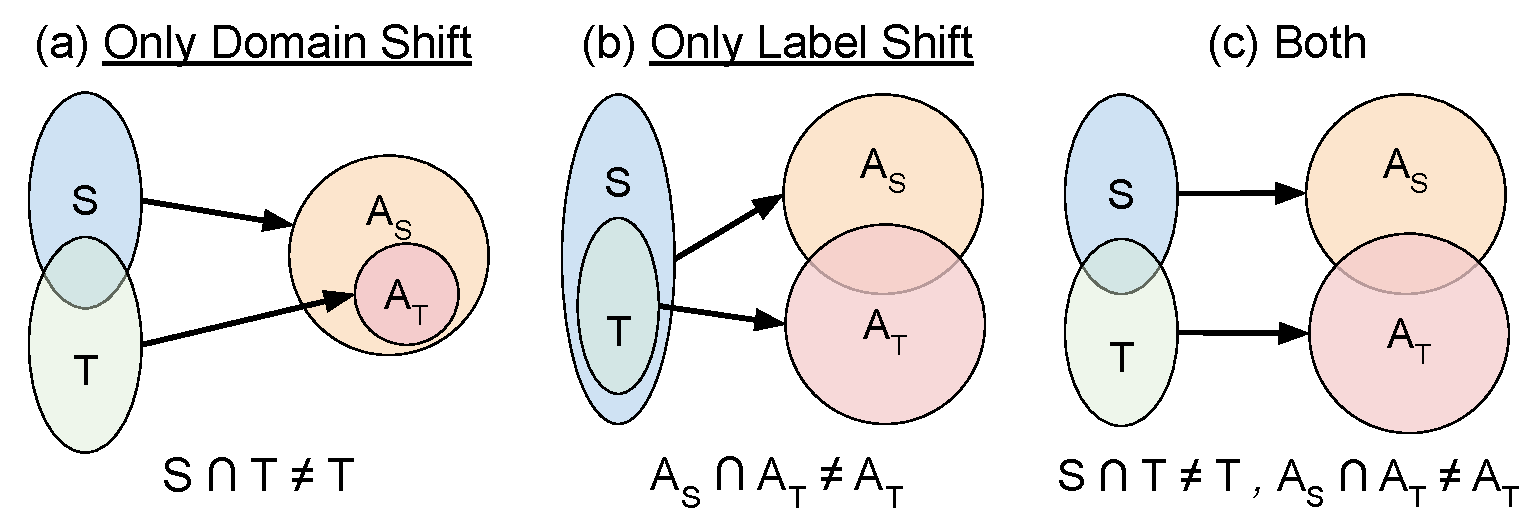
\includegraphics[width=\linewidth]{figures/generalization_types.pdf}
    \caption{Aspects of generalization in VQA.}
    \label{fig:generalization_types}
\end{figure}
The presence of two modalities in V\&L tasks implies that we need to talk about robustness and generalization of V\&L modalities from the perspective of vision, and from the perspective of language.
Most of the robustness literature in V\&L has been for the task of visual question answering.
We review it below.

Robustness in VQA can be defined as shown in Figure~\ref{fig:generalization_types} under two situations: domain shift and label shift.
Under domain shift, generalization to a new input domain (such as different styles of questions or novel scenes) is desired, characterized by $S\cap T \neq T$ where $S$ and $T$ denote the train and test input domains.
Under label shift, generalization to novel answers is desired (predicting answers not seen during training), characterized by $A_S\cap A_T \neq A_T$, where $A_S$ and $A_T$ are the set of answers seen during training and test-time.

Performance under \textbf{domain shift} has been evaluated for new domains of test questions with unseen words and objects~\citep{teney2016zero,ramakrishnan2017empirical}, 
novel compositions~\citep{johnson2017clevr,agrawal2017c}, 
logical connectives~\citep{gokhale2020vqa}, as well as questions that are
implied~\citep{ribeiro-etal-2019-red}, entailed~\citep{ray2019sunny} or sub-questions~\citep{selvaraju2020squinting}; or for datasets with varying linguistic styles~\citep{chao2018cross,xu2019open,shrestha2019answer}
and different reasoning capabilities~\citep{kafle2017analysis}.
Other work seeks to answer target questions that are sub-questions~\citep{selvaraju2020squinting}, or are implied~\citep{ribeiro-etal-2019-red} or entailed~\citep{ray2019sunny} by source questions.
More recently, a new benchmark has been proposed that combines many of the papers mentioned above into a unified evaluation dataset for testing robustness of VQA models~\citep{li2020closer}.


\textbf{Label shift} or Prior Probability Shift~\citep{storkey2009training} has been implicitly explored in VQA-CP~\citep{agrawal2018don}, where the conditional probabilities of answers given the question type deviate at test-time.
% are designed to be different for the train and test shifts.
% \citet{teney2020value} have identified several pitfalls associated with the models and evaluation criteria for VQA-CP.
A similar benchmark for the spatial visual question answering task has been introduced via GQA-OOD~\citep{kervadec2020roses}, which focuses on rare question-answer pairs, and showed that existing VQA models overfitted to dataset biases and underperformed on such OOD questions. 
Similar to GQA-OOD, the VQA-CE dataset~\citep{dancette2021beyond} generated a new evaluation set by using rules to mine questions that can fool existing models.
As for GQA-OOD, this dataset demonstrated that SOTA
models do not perform well when they can’t rely on shortcuts, even models which use bias-reduction
techniques. 
A comprehensive survey of methods that tackle such dataset biases and priors is given by \citet{shrestha2022investigation} and \citet{teney2020value}.





% Approaches such as~\citet{RUBI,teney2019actively,teney2020unshuffling,chen2020counterfactual,gokhale2020mutant} have been recently proposed as solutions to the VQA-CP challenge.
% In the VQA-v2 dataset~\citep{goyal2017making}, questions are created for each image $i \in \mathcal{I}$ by human workers, and the test-train splits are i.i.d. with respect to question-type, and for each question, two images leading to two different answers are collected.
% This is an example of neither domain shift nor label shift.


\chapter{Robustness under Attribute Shift}
\label{chap:agat}
% \begin{abstract}
% While existing work in robust deep learning has focused on small pixel-level norm-based perturbations, this may not account for perturbations encountered in several real-world settings.
% In many such cases although test data might not be available, broad specifications about the types of perturbations (such as an unknown degree of rotation) may be known.
% We consider a setup where robustness is expected over an unseen test domain that is not i.i.d.\ but deviates from the training domain.
% While this deviation may not be exactly known, its broad characterization is specified \textit{a} priori, in terms of attributes.
% We propose an adversarial training approach which learns to generate new samples so as to maximize exposure of the classifier to the attributes-space, without having access to the data from the test domain.
% Our adversarial training solves a min-max optimization problem, with the inner maximization generating adversarial perturbations,
% and the outer minimization finding model parameters by optimizing the loss on adversarial perturbations generated from the inner maximization.
% We demonstrate the applicability of our approach on three types of naturally occurring perturbations -- object-related shifts, geometric transformations, and common image corruptions.
% Our approach enables deep neural networks to be robust against a wide range of naturally occurring perturbations.
% We demonstrate the usefulness of the proposed approach by showing the robustness gains of deep neural networks trained using our adversarial training on MNIST, CIFAR-10, and a new variant of the CLEVR dataset.

% \end{abstract}

%%%%%%%%%%%%%%%%%%%%%%%%%%%%%%%%%%%%%%%%%%%%%%%%%%%%%%%%%%%%%%%%
% \section{Introduction}
%%%%%%%%%%%%%%%%%%%%%%%%%%%%%%%%%%%%%%%%%%%%%%%%%%%%%%%%%%%%%%%%

The goal of \textit{robust} machine learning models for tasks such as image classification is to make accurate predictions on \textit{unseen} samples.
The i.i.d.\ assumption is the simplest case in which unseen samples come from the same distribution as the training dataset.
However, in most real-world situations, this assumption breaks down and so do models trained under the i.i.d.\ paradigm~\citep{recht2018cifar, bulusu2020anomalous}.

As discussed in Chapter~\ref{chap:background}, most prior work on non-\textit{i.i.d.} robustness has been focused on adversarial robustness, i.e. the ability to maintain good performance when the image undergoes pixel-level $\ell_p$ norm-bounded perturbations such as additive noise~\citep{goodfellow2014explaining,sinha2018certifying,madry2018towards,raghunathan2018certified}.
While such perturbations allow the use of tractable mathematical formulations, in practice, they are not the only perturbations that might be encountered at test time.
For example, geometric transforms such as rotation, translation, or scaling of images, that are commonly encountered in the real world are not accounted for by pixel-wise $\ell_p$ bounded perturbations.

Images are parameterized by several unique attributes ranging from low-level information responsible for image formation like lighting, camera angle and resolution; to high-level semantic information like changes in background, size, shape, or color of objects in a scene.
Perturbations along many of these attributes are irrelevant to tasks like image classification and are thus ``semantics-preserving" perturbations.
For instance, translating a digit inside an image in a digit classification task, or manipulating the shape of an object in a color classification task, will not result in a change in the true class-label.
Yet, perturbations along these attributes are likely to cause models to fail when they are changed intentionally or otherwise \citep{xiao2020noise,joshi2019semantic,liu2018beyond}.
Shifts in such ``nuisance attributes'' typically result in large $\ell_p$ perturbations, posing significant challenges for existing pixel-level perturbation models.
On the other hand, it is impractical to sample the entire attribute space effectively in order to guard against potential failures at test time.
In this work, we shall build robust image classifiers that can deal with such types of attribute shift.

The approach that we will discuss in this chapter, is a robust modeling technique that we call \textbf{AGAT: \textit{Attribute Guided Adversarial Training}}, which learns to generate new samples so as to maximize the exposure of the classifier to variations in the attribute space.
Our approach falls under the broad category of adversarial training~\citep{madry2017towards}, and utilizes a min-max optimization setup, wherein the inner maximization step generates adversarial attribute perturbations while the outer minimization step identifies model parameters that reduce the task-specific loss (e.g., categorical cross entropy) under these perturbations.
We find that the attribute-based specification produces models that can more effectively handle challenging real-world distribution shifts than standard $\ell_p$ norm-bounded perturbations~\citep{qiao2020learning}.
Furthermore, our proposed approach is flexible to support a wide-range of attribute specifications, which we demonstrate with three different use-cases:
\begin{enumerate}[nosep,noitemsep,leftmargin=2em]
    \item Object-level shifts from a conditional GAN for adversarial training on a new variant of the CLEVR dataset;
    \item Geometric transformations implemented using a spatial transformer for MNIST data; and
    \item Synthetic image corruptions on CIFAR-10 data.
\end{enumerate}
% Our contributions can be summarized as follows:
% \begin{itemize}[nosep,noitemsep,leftmargin=2em]
%     \item We consider the problem of robustness under a set of specified attributes, that go beyond typically considered $\ell_p$ robustness in the pixel space.
%     \item We present Attribute-Guided Adversarial Training (AGAT), a robust modeling technique that solves a min-max optimization problem and learns to explore the attribute space and to manipulate images in novel ways without access to any test samples.
%     \item We create a new benchmark called ``CLEVR-Singles''
%     to evaluate robustness to semantic shifts. The dataset consists of images with a single block having variable colors, shapes, sizes, materials, and position.
%     \item We demonstrate the efficacy of our method on three classes of semantics-preserving perturbations: object-level shifts, geometric transformations, and common image corruptions.
%     \item Our method outperforms competitive baselines on three robustness benchmarks: CLEVR-Singles, MNIST-RTS, and CIFAR10-C.
% \end{itemize}


% \section{Related Work}
% Most existing work on robustness deals with the problem of finding $\ell_p$ perturbations which focus on additive noise, with tractable mathematical guarantees of performance when test data falls within an $\epsilon$-ball of the training distribution~\citep{goodfellow2014explaining,sinha2018certifying,madry2018towards,raghunathan2018certified}.
% Such perturbation are typically \emph{imperceptible} to the human eye. 
% As a result, there is an increasing interest in addressing challenges that arise from natural corruptions or perturbations \citep{hendrycks2018benchmarking} that are \emph{perceptible} shifts in the data, more likely to be encountered in the real world.
% For example,~\citep{liu2018beyond} use a differentiable renderer to design adversarial perturbations sensitive to semantic concepts like lighting and geometry in a scene;~\citep{joshi2019semantic} design perturbations only along certain pre-specified attributes by optimizing over the range-space of a conditional generator. 
% Our work focuses on building robust models against semantic, or more generally attribute guided concepts that may or may not exist in the training distribution, using a surrogate function. 

% $\ell_p$-norm based robustness methods make no assumptions about the test distribution, except that the methods are guaranteed to be robust only inside the $\epsilon$-ball of the training distribution~\citep{volpi2018generalizing,qiao2020learning}.
% Some recent approaches extend this notion to assume some access to data from the test distribution such as TTT~\citep{sun2020test} that achieves robustness for a test example by minimizing the cost of an auxiliary task for each test sample; and~\citep{wong2020learning} learn a CVAE using possible corruptions one might encounter, to then guarantee robustness of a classifier within the learned perturbation set.
% For comparison, our method assumes access to no data from the test distribution, but only knowledge of a specification, which is the intended functionality of the system specified in human-understandable attributes. Under this challenging set-up, we show our method still outperforms existing robustness techniques on popular and standard benchmarks. 


\section{Setup}
\begin{figure}
    \centering
    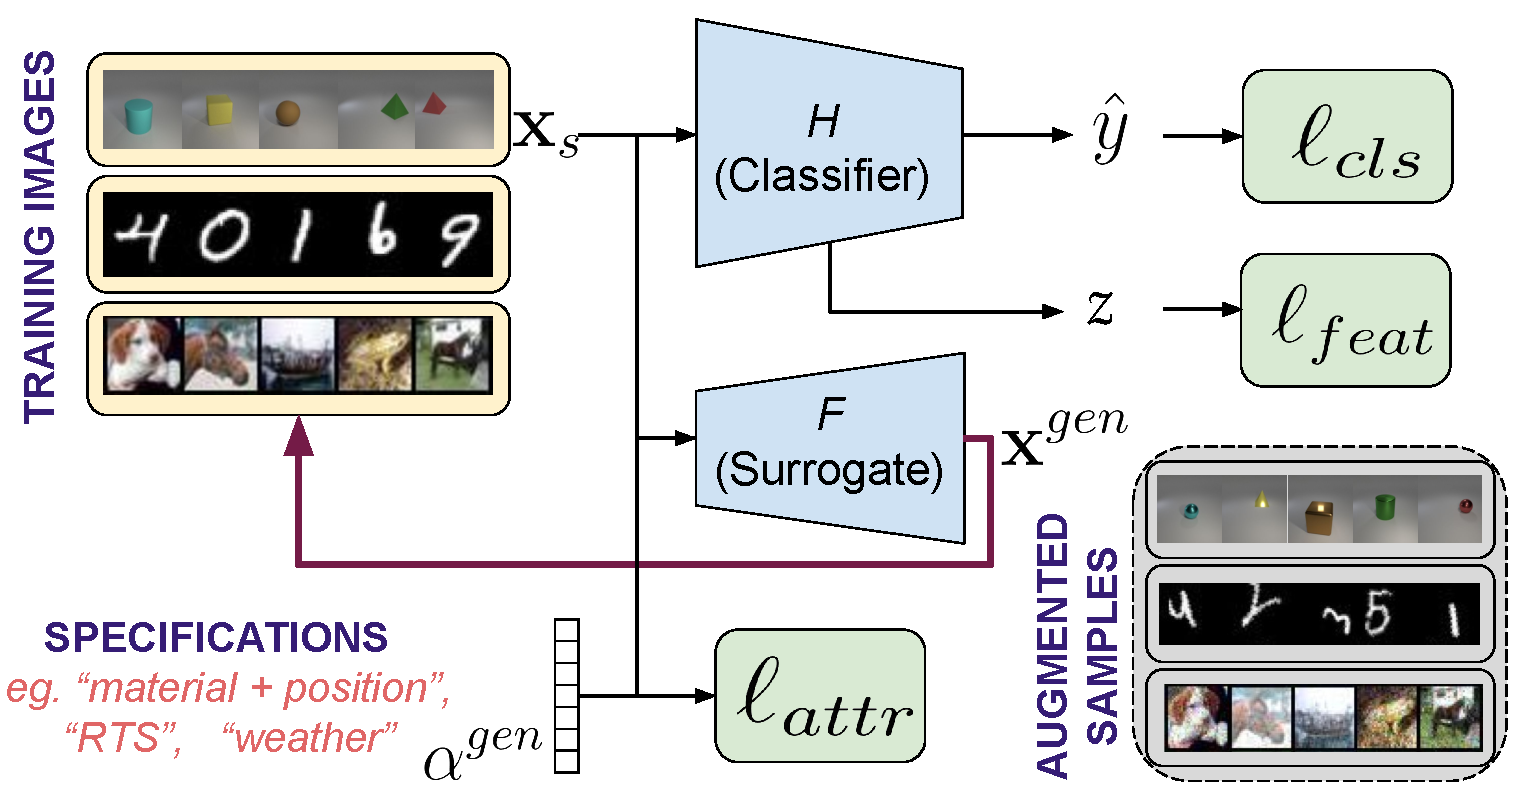
\includegraphics[width=\linewidth]{agat/images/overall_new.pdf}
    \caption{Overview of the problem setup and our attribute-guided adversarial training method.}
    \label{fig:problem}
\end{figure}


We begin by defining the classifier parameterized by a set of neural network weights, $\theta$, as
${H}_{\theta}:
\mathcal{X}_s\mapsto \mathcal{Y}$, where $\mathcal{X}_s$ denotes the space of the observed image data (or source) and $\mathcal{Y}$ denotes the label space for the task of interest.

\paragraph{Robustness to natural perturbations.}
Our goal is to train an $H_{\theta}$ that is robust to \emph{natural} perturbations, which are typically larger in magnitude than the \emph{imperceptible} $\ell_p$-bounded pixel-space perturbations, considered in the literature.
We will consider sementic shifts in attributes such as shape, size, texture, and position of objects; geometric transformations of varying internsities; and common image corruptions such as noise, blur, weather, and digital artifacts.
% We consider a broad range of natural semantics-preserving perturbations that will not affect the predictions for the task under consideration --
%     (a) \textbf{Object-level shifts}, where attributes of the object are
%     manipulated so as to considerably change the appearance of the object, without changing the task label; such as changing the shape or size of an object in a color classification task.
%     % \BK{This definition should be changed Semantic Invariant}
%     (b) \textbf{Geometric transformations}, where the test image may be scaled, rotated, and shifted in arbitrary ways; and
%     (c) \textbf{Common image corruptions}, which may occur in the real world like fog, image compression artifacts, blurs, and other forms of noise.
Most of these perturbations do not naturally fall within small $\ell_p$-norm ball deviations ($|\mathbf{x}-\tilde{\mathbf{x}}|_p\leq \epsilon$), for which most existing robustness methods are designed, and are bound to fail when the classifier encounters such data in the wild.
However, making $\epsilon$ arbitrarily large in robustness formulations does not work in practice, since the image quality degrades significantly. 
Hence, we propose a new framework to design models that are robust to such natural perturbations.

\section{Attribute Guided Adversarial Training}

Let us denote an image by $\mathbf{x}_\alpha$ parameterized by a set of attributes $\alpha$ related to image formation (lighting, viewing angle, position) as well as abstract semantic information (color, shape, size, etc.). 
Manipulating images with new combinations of attributes that are not seen in the training set, requires access to the underlying physical generative processes,  which is unrealistic. We do not assume direct access to such deterministic mechanisms.

Our goal is to train classifiers robust to natural perturbations along 
% nuisance 
attributes in $\alpha$ that are specified \emph{a priori}. Inspired by recent developments in robust optimization and adversarial training~\citep{madry2018towards}, we consider the following worst-case problem around $N$ attributes of the training data:
\begin{equation}
    \min_{\theta\in \Theta}\sum_{i=1}^N\max_{|\hat{\alpha}_i-\alpha_i|\leq \epsilon} \ell(\theta;(\mathbf{x}_{\hat{\alpha}_i},y_i)),
    \label{agat:eq:adv_training_worst_case}
\end{equation}
where $\ell(\cdot)$ is the cross-entropy loss.

The solution to worst-case optimization in Equation~\ref{agat:eq:adv_training_worst_case} guarantees good performance against test data that is distance $\epsilon$ away from the training data in the attribute space. 
In other words, we expect the model learned using \eqref{agat:eq:adv_training_worst_case} to be robust against $\epsilon$-bounded natural perturbations.
Interestingly, as we will empirically show later, models learnt using \eqref{agat:eq:adv_training_worst_case} perform better than existing pixel-level techniques even on $\ell_p$-bounded imperceptible perturbations.

Although the structure of the attribute-guided adversarial training problem may look similar to standard adversarial training, we explain next why solving Eq~\eqref{agat:eq:adv_training_worst_case} is significantly more challenging and requires us to make several algorithmic innovations. 
Note that \eqref{agat:eq:adv_training_worst_case} solves a min-max optimization problem, with the inner maximization generating natural perturbations by maximizing the classification loss over attribute space, and the outer minimization finding model parameters by minimizing the loss on natural perturbations of the training data generated from the inner maximization. The success of this method crucially relies on solving the inner optimization problem. 
Motivated by the standard adversarial training, one might be temped to approximately solve the re-parameterized inner optimization problem
\begin{equation}
    \underset{|{\delta}|_p\leq \epsilon}{\max}~~l(\theta;(\mathbf{x}_{{\alpha}_i+{\delta}},y_i)),
\end{equation}
and generate the natural perturbations
$\mathbf{x}_{\hat{\alpha}_i}^*$
using projected gradient descent (PGD) as:
\begin{equation}
    {\delta_i}^* := \mathcal{P}_{\epsilon} (\delta_i-\lambda \nabla_{\delta} l(\theta;(\mathbf{x}_{{\alpha}_i+{\delta}},y_i))),
\end{equation}
where $\lambda$ is the gradient step and $\mathcal{P}_{\epsilon}$ is projection on $l_p$ ball of radius $\epsilon$. However, there are two fundamental issues with this approach making it infeasible in practice: first, we cannot compute gradients as we do not have access to the attribute space;
and second, we do not have access to the true generative mechanism conditioned on the attributes.

\subsection{Proposed Approach}
\paragraph{Surrogate Functions.}
We propose to use differentiable surrogate functions parameterized by attributes to overcome the limitation described above. 
In other words, we have 
$\mathbf{x}_{\alpha+\delta} \approx F_{\delta}(\mathbf{x}_{\alpha})$, 
where $F_{\delta}$ is differentiable.
Typically, exact perturbations 
$\mathbf{x}_{\alpha+\delta} = F_{\delta}(\mathbf{x}_{\alpha})$
can be performed for PGD attacks or other $\ell_p$ norm bounded attacks.
However, in our case accessing the true generative process to manipulate images along $\alpha$ is not feasible. 
For example, we cannot rely on deterministic functions to manipulate semantic features in the image like size, shape or texture of an object.
As a result, we resort to using \emph{approximate} image manipulators in the form of surrogate functions which act as proxies to the true generative process.
Depending on the type of attributes against which we wish to train for robustness, the surrogate function can take different forms:
\begin{itemize}[nosep,noitemsep,leftmargin=2em]
    \item generative editing models for semantic perturbation that is learned from the training data itself,
    \item analytical functions for geometric transformations in the form of spatial transformers (STNs), or 
    \item an analytical approximation (or tractable upper bound) of the natural perturbation space.
\end{itemize}
For example, if we want a classifier robust to unknown affine transforms then $F$ is the spatial transformer layer parameterized by $\alpha$ which now represents $6$ parameters controlling rotation, scale, and shift of the image.




Note that we do not assume access to any additional data other than the clean training dataset $\mathcal{X}_s$, and specification of the class of functions against which robustness is desired. While such surrogate functions only approximate the natural perturbations, we show that they are sufficient for enabling us to make classifiers more robust to natural perturbations.




\paragraph{Iterative Training Procedure.}
Having access to attribute parameterized surrogate function, we aim to solve \eqref{agat:eq:adv_training_worst_case}. Note, the success of the adversarial training is dependent on the quality of the generated perturbations. Thus, we aim to generate natural perturbations that have a larger coverage over the specified attribute space than the training samples images $\mathbf{x}_s$. Consider the classifier $H_\theta$ which outputs the predicted class $\hat{y}$ and intermediate features $z$, let the surrogate function ${F}$ be parameterized by the attribute vector $\alpha$. We propose an iterative training procedure called Attribute-Guided Adversarial Training (\textbf{AGAT}) detailed in Algorithm~\ref{alg:adv_algo}. Our algorithm has two objectives: to minimize the classification loss over input images and to maximize the divergence between the training samples and generated perturbations. Thus, the key idea here is to explore novel and hard images that only \emph{vary along the specified attributes}. To achieve this, we impose a constraint that maximizes the distance between features of dataset images and perturbed images. Additionally, since we would also like to explore new regions in the attribute space, we impose a similar constraint on the attributes of perturbed images.


We express this constraint as the loss function given by:
\begin{equation}
    \begin{split}
        \ell_{const} = \lambda_1\ell_{feat} + \lambda_2\ell_{attr},~~\lambda_1, \lambda_2 \in (0,1)\\
        \text{where~~ }
        \ell_{feat} = ||\mathbf{z} - \mathbf{z^{gen}}||_2^2,
        \text{~and~~}
        \ell_{attr} = ||\alpha - \alpha^{gen}||_2^2
    \end{split}
    \label{agat:eq:loss_constraint}
\end{equation}


To ensure that the generated images belong to the same class as the input image, we combine classification loss with respect to the ground truth label $\mathbf{y}$ with consistency regularization with respect to the predicted label $\mathbf{\hat{y}}$ of $\mathbf{x}$.
\begin{equation}
    \ell_{cls} = \ell_{BCE}(\mathbf{y}, \mathbf{y^{gen}}) + \ell_{BCE}(\mathbf{\hat{y}}, \mathbf{y^{gen}})
    \label{agat:eq:loss_distill}
\end{equation}


\noindent The overall loss function is computed as the Lagrangian:
\begin{equation}
    \ell_{AGAT} = \ell_{cls} - \beta\cdot\ell_{const}
    \label{agat:eq:loss_overall}
\end{equation}

\begin{algorithm}
    \caption{Attribute-Guided Adversarial Training}
    \label{alg:adv_algo}
    \small
    % \begin{algorithmic}[0]
    %     % \REQUIRE $n \geq 0 \vee x \neq 0$
    %     \State \textbf{Input:} Source dataset $\mathcal{D}_S=\{\mathbf{x}_t,y_t\}_{i=t}^T$
    %     \State \textbf{Output:} learned weights $\theta$ 
    % \end{algorithmic}
    \begin{algorithmic}[1]
        \State \textbf{Initialize:} $\theta \gets \theta_0, \mathcal{D}^{aug}_S\gets\mathcal{D}_S$
        \ForEach{$n=1\dots N_{epochs}$}
            \If{$n < N_{pre}$}
                \ForEach{$t=1:T$}
                    \State $\theta \gets \theta - \eta\triangledown\ell_{cls}(\theta;(\mathbf{x}_t, y_t))$
                \EndForEach
            \Else
                \If{$n~\text{mod }N_{aug} = 0$}
                    \ForEach{$t=1\ldots T_{aug}$}
                        \State sample ${(\mathbf{x}_t, y_t)}_{t=1}^{T_{aug}}$ from $\mathcal{D}_S$
                        \State $z_t, \hat{y}_t = H(\mathbf{x_t})$
                        \State \textbf{Initialize:} $\alpha_t^{gen}$
                        \ForEach{$i=1\ldots M$}
                            \State $z^{gen}_t, \hat{y}^{gen}_t = H(\mathbf{x}_t, \alpha_t^{gen})$
                            \State $\mathbf{x}_t^{gen} \gets f(\mathbf{x}_t, \alpha_t^{gen})$
                            \State $\alpha_t^{gen} \gets \alpha_t^{gen} - \mu\triangledown (\cdot\ell_{cls}-\beta\cdot \ell_{cons})$
                        
                        \EndForEach
                        
                        \State $\mathcal{D}_S^{aug} \gets \mathcal{D}_S^{aug} \cup \mathbf{x}_t^{gen}$
                    \EndForEach
                \Else
                    \ForEach{$(\mathbf{x}_t, y_t) \in \mathcal{D}^{aug}_S$}
                         \State $\theta \gets \theta - \eta\triangledown\ell(\theta;(\mathbf{x}_t, y_t))$
                    \EndForEach
                \EndIf
            \EndIf
        \EndForEach
    \end{algorithmic}
\end{algorithm}
%     
% \State $\ell_{feat} = $ 
% \State $\ell_{attr} = $ 
% \State $L = \ell_{feat}(z_t, z_t^{aug}) + \ell_{cls}(\theta;(X_t, y_t))$
% \State $\ell_{tot} = \alpha\cdot\ell_{dis}(y_t, \hat{y}_t, \hat{y}_t^{aug}) - \beta c(z_t, z_t^{aug}, b_t, b_t^{aug})$

% \BK{Notations below and in algo should be consistent with the previous section}
Intuitively, $\ell_{cls}$ encourages the augmented images to belong to the same class-label as the input image, while the constraint $\ell_{const}$ encourages the adversarial learning algorithm to perturb the image features as well as the attributes away from the input features and attributes.
We first pre-train the classifier only on the source samples $\mathbf{x}_s$ for $N_{pre}$ epochs.
Then, we initiate our augmentation process.
To generate new samples, we minimize Equation~\ref{agat:eq:loss_overall} and update the attribute vector for $M$ update steps as:
\begin{equation}
    \alpha^{gen} \gets \alpha^{gen} - \mu\triangledown \ell_{AGAT}.
\end{equation}
Finally, synthetic images are generated using the surrogate function 
\begin{equation}
    \mathbf{x}^{gen} \gets F(\mathbf{x}, \alpha^{gen}), 
\end{equation}
These generated images are then appended to the training data.
This adversarial data augmentation is performed after every $N_{aug}$ epochs during which $T_{aug}$ images are generated.
The total number of augmented samples is expressed as a percentage of the number of training samples so as to allow fair comparison across datasets and types of perturbations.
The pseudocode for AGAT is shown in Algorithm~\ref{alg:adv_algo}.


The distinguishing factor for \textbf{AGAT} is that we perturb the attribute space and use surrogate functions to synthesize images, while previous adversarial augmentation protocols such as M-ADA~\citep{qiao2020learning} and GUD~\citep{volpi2018generalizing} perturb only in the pixel-space, thus being restricted to $\ell_p$ perturbations.
It is important to note that our method is agnostic to the choice of surrogate functions, which can take the form of additive noise, affine transformation in pixel-space, or conditional generative adversarial networks~\citep{mirza2014conditional} trained to transform an input image according to an input attribute vector.


\section{Experiments}
In this section, we introduce the three types of robustness specifications that we experiment with, along with details about the datasets, baselines, and metrics used for each.

\begin{figure}[t]
    \centering
    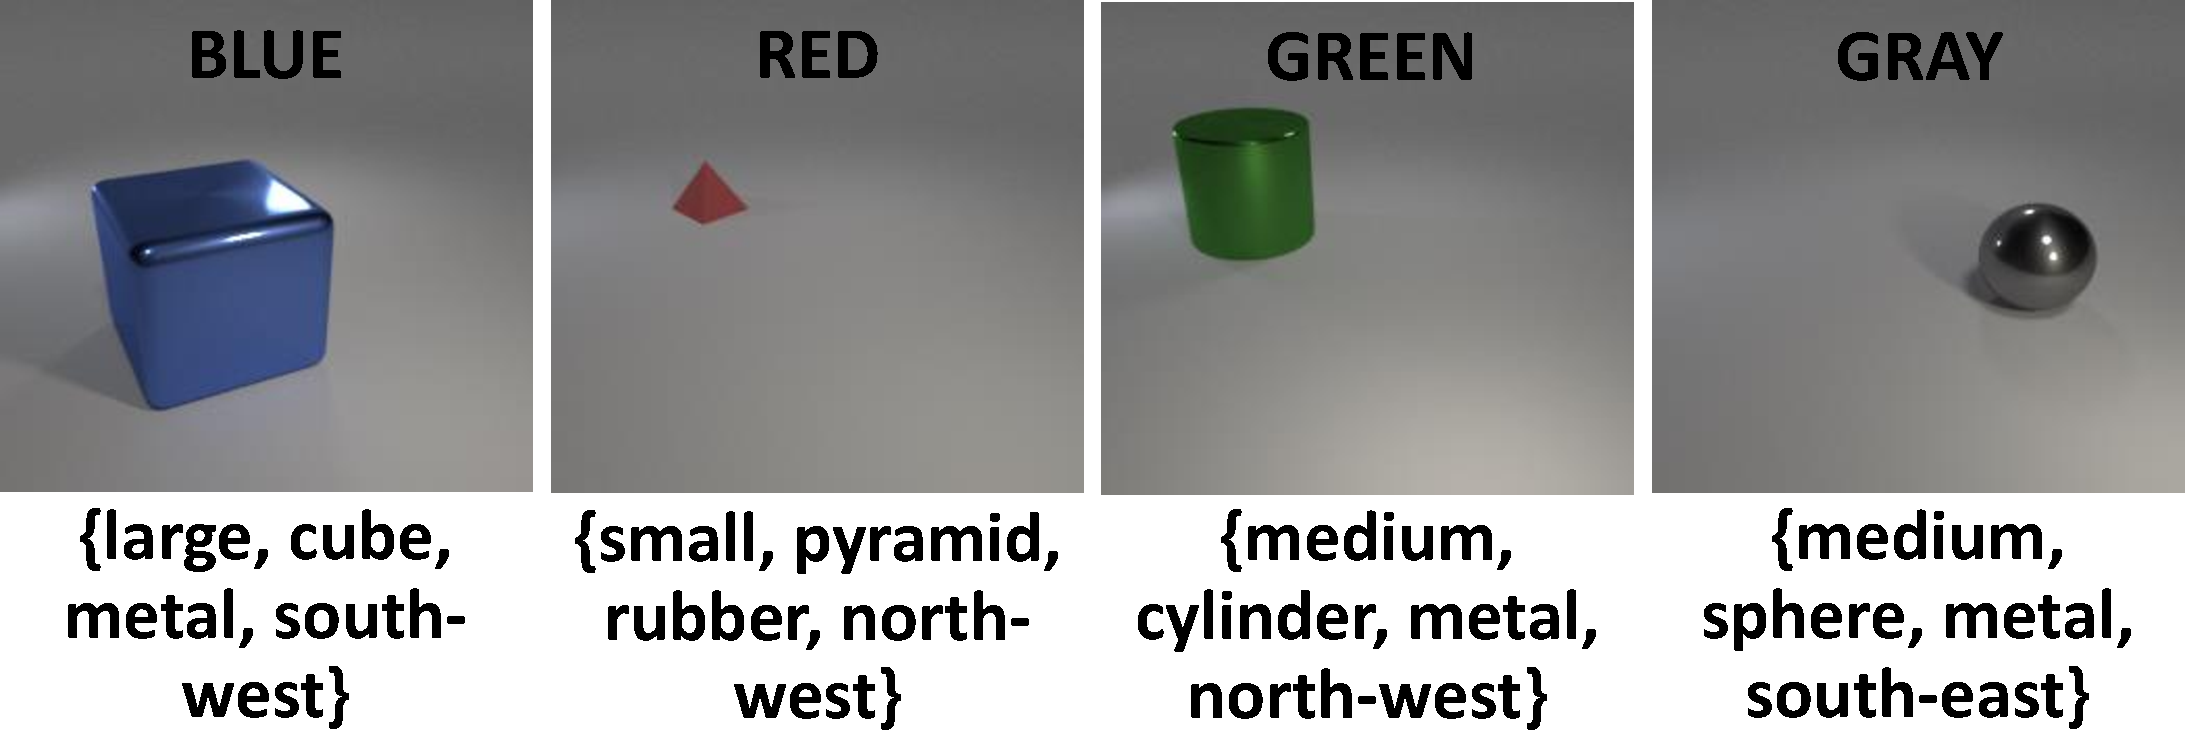
\includegraphics[width=0.99\linewidth]{agat/images/clevr_singles.pdf}
    \caption{Examples of images from CLEVR-Singles and the color labels and (size, shape, material, position) attributes.}
    \label{fig:clevr_singles}
\end{figure}

\begin{table}
    \centering
    \small
    \resizebox{\linewidth}{!}{   
    \begin{tabular}{@{}p{0.24\linewidth}p{0.35\linewidth}p{0.35\linewidth}@{}}
        \toprule
        \textbf{Attribute} & \textbf{Train} & \textbf{Test} \\
        \toprule
        
        {{Size and Position}} & {(small, NW), (medium, NE), (large, SE)} & {(small, SE), (medium, NW), (large, SW)} \\
        \midrule
        {Material and Position} & {(metal, NW), (rubber, NW), (metal, NE), (rubber, NE)} & (rubber, SW), (metal, SW), (rubber, SE), (metal, SE)\\
        \bottomrule
    \end{tabular}
    }
    \caption{The train and test splits for our experiments with semantic object-level perturbations for CLEVR-Singles.}
    \label{tab:clevr_splits}
\end{table}

\begin{figure}[t]
    \centering
    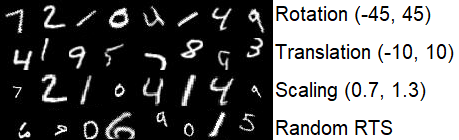
\includegraphics[width=0.75\linewidth]{agat/images/mnist_rts_bigfont.png}
    \caption{
    RTS-perturbed MNIST images.
    }
    \label{fig:mnist_rts}
\end{figure}


%%%%%%%%%%%%%%%%%%%%%%%%%%%%%%%%%%%%%%%%
\subsection{Semantic Object-Level Perturbations}
One class of real-world perturbations is when properties or attributes of images or objects in images change at test time.
These changes do not affect the classification label, but significantly change the appearance of the image.
For instance, consider the task of color classification in objects of varied shapes and textures. 
Here, \textit{red metallic spheres} and \textit{red rubber cubes} both belong to the class label ``red", however may appear very different in their shapes and textures. 
Thus, if only \textit{red metallic cubes} are seen during training, conventional classifier predictions for test images consisting of \textit{red rubber cubes} can fail to generalize. 
Thus, although the class label is invariant to such semantic factors, robustness to perturbations along these factors is desirable.

    \paragraph{Dataset:}

    To study the problem of such object-level shifts along semantic factors of an image in a controlled fashion, we create a new benchmark called CLEVR-Singles\footnote{
        Dataset: \url{https://github.com/tejas-gokhale/CLEVR-Singles}} 
    by modifying the data generation process from CLEVR~\citep{johnson2017clevr}.
    We create images of single objects having one of eight colors, and use color classification as our task in this paper.
    Each object has four variable attributes that do not affect the color class of the image; these are: \textit{shape} (cube, sphere, pyramid, or cylinder), \textit{size} (small, medium, or large), \textit{material} (rubber or metal), and \textit{position} (northwest, southwest, northeast, southeast).
    While the objects are generated at continuous $(X, Y, Z)$ world coordinates, we assign them a discrete position class for our experiments.
    Object-level perturbations can be made over these four attributes for our robustness experiments.
    In other words, it is known that one or more of \textit{\{shape, size, material, position\}} of the image may change at test-time without knowing the magnitude or combinations of the change.
    We split the dataset based on a combination of attributes as shown in Table~\ref{tab:clevr_splits}; for instance only certain combinations of size and position are observed in the training set, but robustness is expected from the color classifier on unknown combinations.

    \paragraph{AttGAN as the Surrogate Function:}
    \begin{figure}
        \centering
        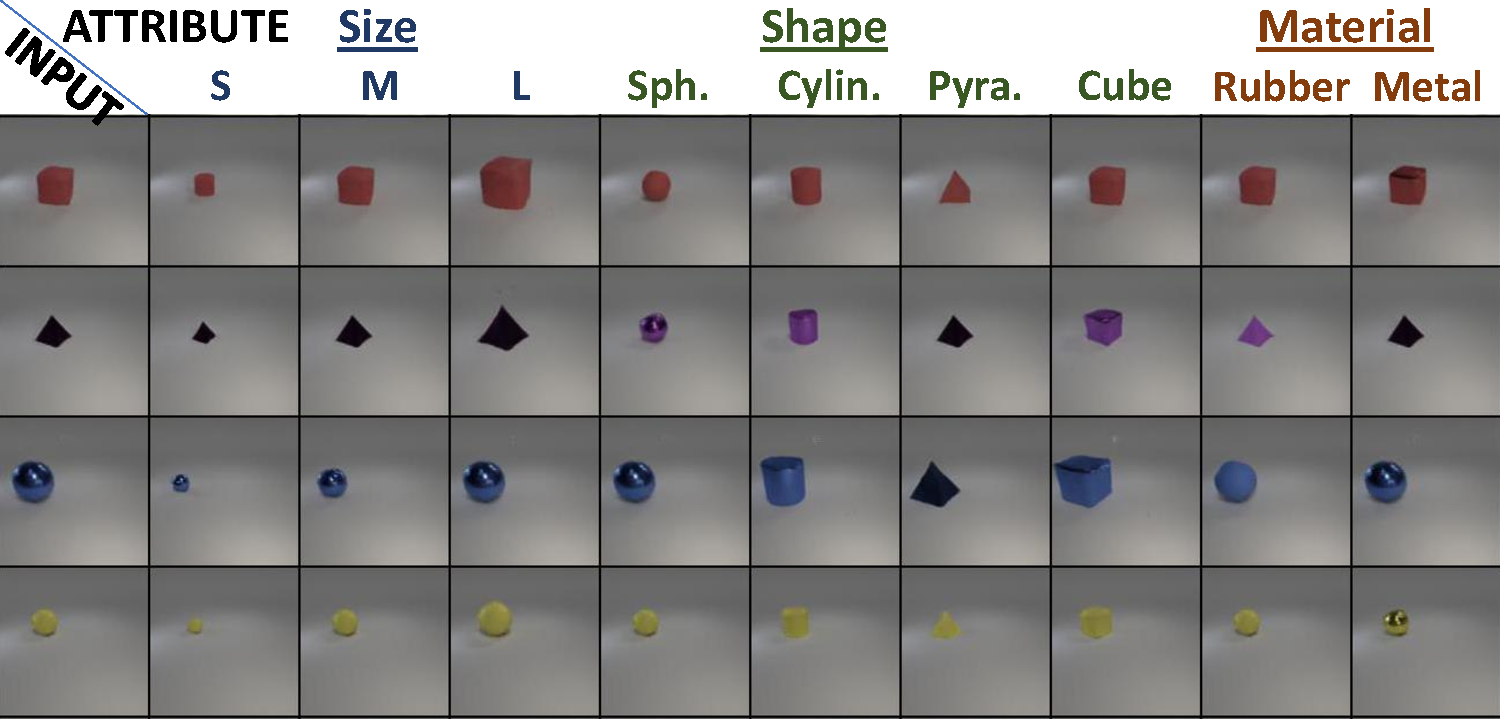
\includegraphics[width=\linewidth]{agat/images/attgan_outputs.pdf}
        \caption{Images generated by AttGAN for the images in column 1, conditioned on attributes.
        % : size(2-4), shape (5-8), material (9-10)
        }
        \label{fig:attgan}
    \end{figure}
    Conditional generative adversarial networks (cGANs) have been shown to perform exceptionally well on image-to-image translation in various domains~\citep{isola2017image,zhang2017stackgan,karras2019style}.
    AttGAN~\citep{he2019attgan} is one such conditional GAN which is trained to manipulate attributes of input face images.
    Thus given an image and a vector of desired attributes, AttGAN can manipulate the face image along the desired attribute dimensions.
    We leverage this powerful image manipulation technique as our surrogate function $\mathbf{x}^{gen} = F_{GAN}(\mathbf{x}, \alpha)$.
    Formally, we define the attribute vector to be a 13-dimensional binary hash-code with 1 and 0 indicating presence or absence of an attribute.
    For each experiment, we train the AttGAN on the training dataset outlined in Table~\ref{tab:clevr_splits} to generate 128x128 images, with a learning rate of $2\mathrm{e-}4$ for 100 epochs on a single 16GB GPU.
    Examples of images generated by AttGAN are shown in Figure~\ref{fig:attgan}, when manipulating certain attributes such as size, shape, and material of the object.

    \paragraph{Baselines:}
    For the color classification task on CLEVR-Singles images, we compare against two pixel-level domain augmentation baselines: GUD~\citep{volpi2018generalizing} which performs adversarial data augmentation to generate fictitious target domains, and M-ADA~\citep{qiao2020learning} which uses a meta-learning framework to generate multiple domains of samples.
    We also report the performance of a classifier directly without any adversarial training as a naive baseline.
    The same classifier architecture is used for each baseline for fair comparison.
    All models are trained for $15$ epochs including pre-training epochs $N_{pre}=5$, batch-size $64$, and $M=15$ update steps for adversarial augmentation.
    The number of augmented samples $T_{aug}$ is $30\%$ of the original source data, and augmentation interval $N_{aug}$ is fixed at 2 epochs.
    For our model the coefficients in Equations~\ref{agat:eq:loss_constraint}, and~\ref{agat:eq:loss_distill} are: $\lambda_1=0.5, \lambda_2=0.5, \beta=0.25$.
    The learning rates $\eta, \mu$ for the classifier and adversarial augmentation are both 5e-5. %$5\mathrm{e-}5$.

    \paragraph{Results:}
    \begin{table}
    \centering
    % \small
    % \resizebox{\linewidth}{!}{
    \begin{tabular}{@{}lccc@{}}
        \toprule
        \textbf{Method} & \textbf{Source} & \textbf{Size + Position} & \textbf{Material + Position} \\ 
        \midrule
        Baseline (ERM)           & 99.81 & 89.92 & 59.90 \\
        GUD~\citep{volpi2018generalizing}         & 99.94 & 93.69 & 65.03 \\
        % M-ADA (K=1) & 99.93 & 95.65 &  \\
        M-ADA~\citep{qiao2020learning}      & 99.96 & 94.52 & 65.50 \\
        Ours        & 99.97 & 95.22 & 69.49 \\ 
        \bottomrule
    \end{tabular}
    % }
    \caption{Classification accuracy for color-classification on CLEVR-Singles. 
    Source and target sets are split on \textit{size+position} attribute for the third column, and \textit{Material+Position} for the fourth column.}
    \label{tab:clevr_results}
\end{table}
    The test classification accuracies for different splits are reported in Table~\ref{tab:clevr_results}. 
    We observe that our model is better than all baselines considered here, with a boost of $5$ percentage points in accuracy on the harder experiment along \textit{Material+Position}.
    


    \paragraph{Analysis:}
    \begin{figure}[t]
        \centering
        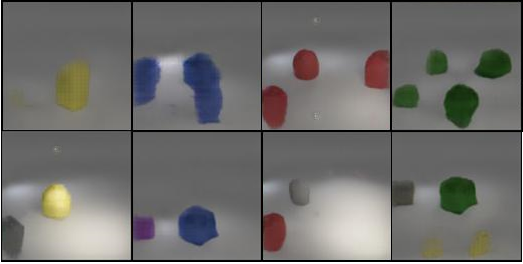
\includegraphics[width=0.58\linewidth]{agat/images/clevr_beta_viz.png}
        \caption{Visualization of the effect of weight $\beta$ of the constraint loss $\ell_{const}$ on the generated images. Row 2 has higher $\beta$ than Row 1. Illustration also shows that AttGAN is able to generate multiple objects (of same color for Row 1 and different colors for Row 2), though absent in training data.
        }
        \label{fig:clevr_novel_viz}
    \end{figure}
    

    In Figure~\ref{fig:clevr_novel_viz}, we show 8 different examples generated by AttGAN during adversarial training. We can see the effect of the coefficient $\beta$, from the constraint loss $\ell_{const}$ in eq~\eqref{agat:eq:loss_overall}, in exploring the attribute space. An appropriately chosen value for $\beta$ encourages useful perturbations without violating the class-label consistency cost $\ell_{cls}$ as seen in the top row of Figure \ref{fig:clevr_novel_viz}. On the other hand, a higher $\beta$ would mean a higher weight for exploring the regions (or combinations) in attribute space not seen in training. In the bottom row we see that a high $\beta$ encourages novel attribute exploration at the cost of higher classification error as a result of generating objects with different colors within the same image.  It is noteworthy that AttGAN is able to generate images with multiple objects, even when it trained on images with only a single object, thus demonstrating its suitability to explore novel attributes using the proposed AGAT training.

%%%%%%%%%%%%%%%%%%%%%%%%%%%%%%%%%%%%%%%%
\subsection{Geometric Transformations}
Another common class of perturbations is geometric transformations, i.e. a composition of rotation, translation, and scaling of an image. These perturbations are common since cameras may capture a scene from different orientations, distances, and inclinations. It is well known that standard image classifiers are not robust to these common perturbations~\citep{cohen2014transformation}.

    \paragraph{Dataset:}
    We address this problem in the digit classification setting, with
    the training images from MNIST~\citep{lecun1998mnist}, and the test images that are perturbed along rotation-translation-scale (RTS), as shown in Figure~\ref{fig:mnist_rts}.
    We use the standard RTS setup~\citep{jaderberg2015spatial} with angle of rotation in $(-45, 45)^{\circ}$, translation in $(-10, 10)$ pixels in both directions, and a scale factor in the range $(0.7, 1.3)$.

    \paragraph{Surrogate Function:}
    The attributes of interest, $\alpha$, consist of a $2\times3$ affine matrix that controls rotation, translation, and scale. To perform affine transformations on the image with a perturbed $\alpha$, we use Spatial Transformer Networks (STN)~\citep{jaderberg2015spatial} which allow differentiable spatial manipulation of input images in a convolutional neural network, such as RTS and or general warping. The perturbed images are generated as: $\mathbf{x}^{gen} = F_{STN}(\mathbf{x}_s, \alpha)$.

    \paragraph{Baselines:}
    We compare the robustness performance to RTS perturbations with a naive baseline, denoted by (B), that is only trained on the standard MNIST dataset, and pixel-level perturbation methods MADA~\citep{qiao2020learning} and GUD~\citep{volpi2018generalizing}.
    Additionally, we also use the RTS perturbation sets generated by~\citep{wong2020learning} (PS) and use them as augmented training samples. 
    All models are trained for 12 epochs including pre-training epochs $N_{pre}=5$, with a batch-size $64$, and $M=10$ update steps for adversarial augmentation. The number of augmented samples $T_{aug}$ is $30\%$ of the original source data, and augmentation interval $N_{aug}$ is fixed at 10 epochs.
    Our model the coefficients in Equations~\ref{agat:eq:loss_constraint}, and~\ref{agat:eq:loss_distill} are: $\lambda_1=1, \lambda_2=1, \beta=5$.
    The learning rate $\eta$ for the classifier is $1\mathrm{e-}4$ and $\mu$ for the adversarial augmentation is $0.1$.


    \paragraph{Results:}

    \begin{table}
    \centering
    % \small
    % \resizebox{\linewidth}{!}{
    \begin{tabular}{@{}l@{\extracolsep{\fill}}cccc@{}}
        \toprule
        \textbf{Method} & \textbf{R} & \textbf{T} & \textbf{S} & \textbf{RTS}\\
        \toprule
        B & 84.44 & 27.67 & 95.76 & 21.91 \\
        GUD~\citep{volpi2018generalizing} & 86.08 & 29.09 & 97.89 & 23.10 \\
        % MADA (K=1) & 87.69 & 28.32 & 98.47 & 22.62 \\
        MADA~\citep{qiao2020learning} & 87.37 & 29.25 & \textbf{98.32} & {22.68} \\
        PS~\citep{wong2020learning} & \textbf{87.86} & 45.36 & 96.00 & 39.38 \\
        Ours ($T_{aug}\text{=}30\%$) & \underline{84.93} & \underline{\textbf{52.95}} & \underline{96.11} & \textbf{\underline{41.43}} \\
        % PS(\%aug=50) & 87.86 & 45.36 & 96.00 & 39.38 \\
        % Ours (\%aug=50) & 86.35 & 61.07 & 95.76 & 47.59\\
        \bottomrule
    \end{tabular}
    % }
    \caption{Results on the MNIST-RTS robustness benchmark for rotation (R), translation (T), scaling (S), and random combination (RTS).}
    \label{tab:mnist_geom}
\end{table}

    We report digit classification accuracies on the target test set containing only rotations (R), only translations (T), only skew (S), as well as a random combination of RTS. Our model performs well on all four metrics, and beats the perturbation sets (PS) even though their augmentation model has access to RTS perturbations during training. In particular, we observe a significant improvement compared with MADA and GUD, in the robustness on the translation experiment, which is the hardest task among the three. 

    \paragraph{Analysis:}
     \begin{figure*}
        \centering
        % 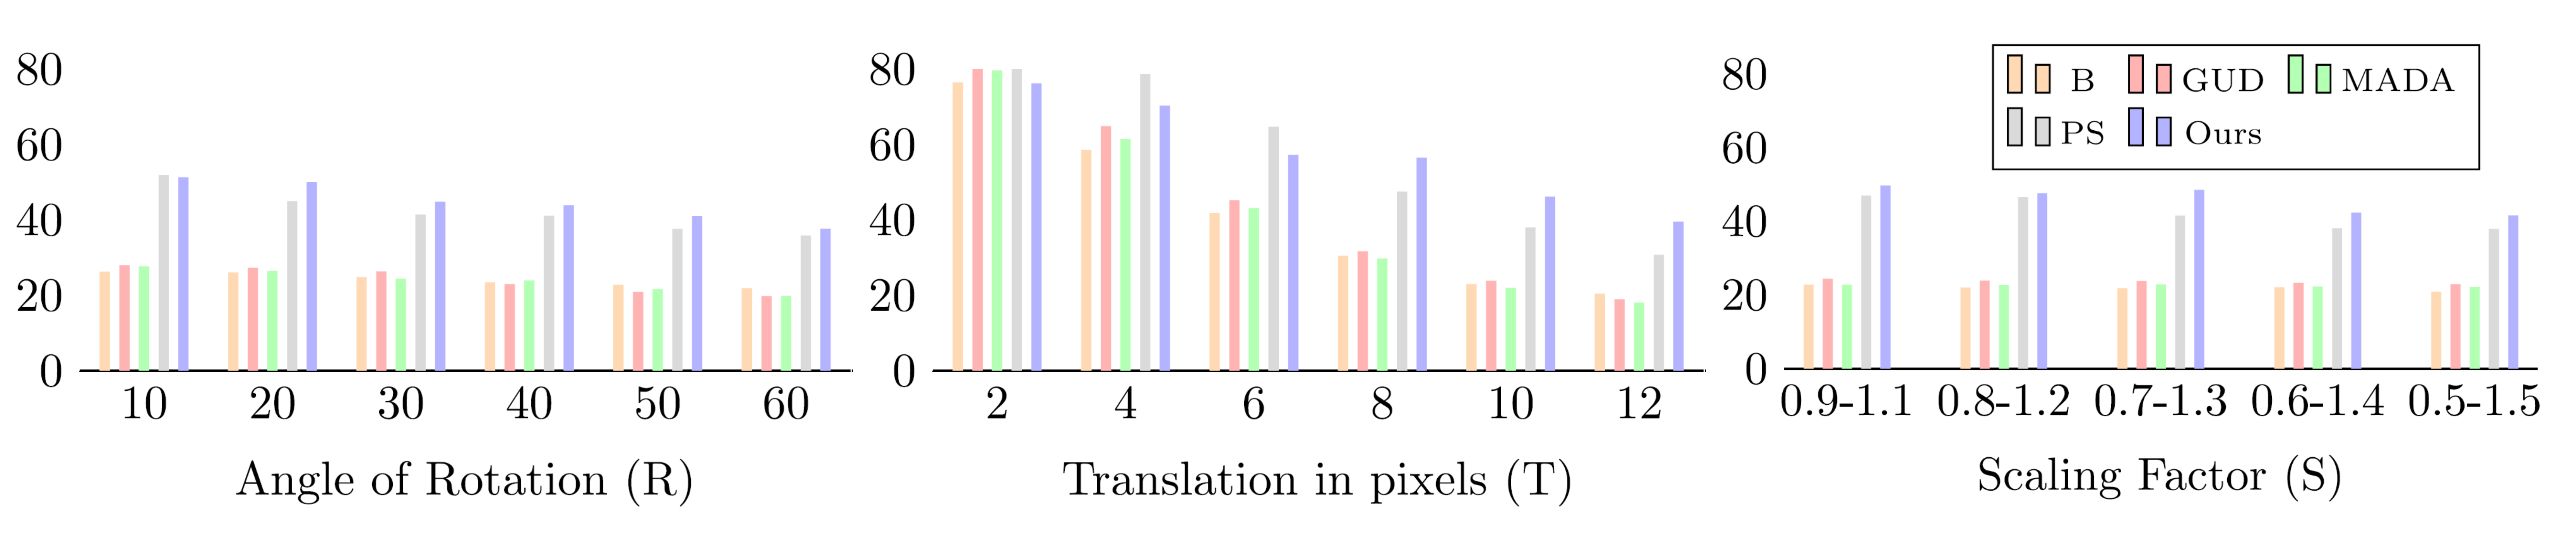
\includegraphics[width=0.93\linewidth]{agat/images/ablation.png}
        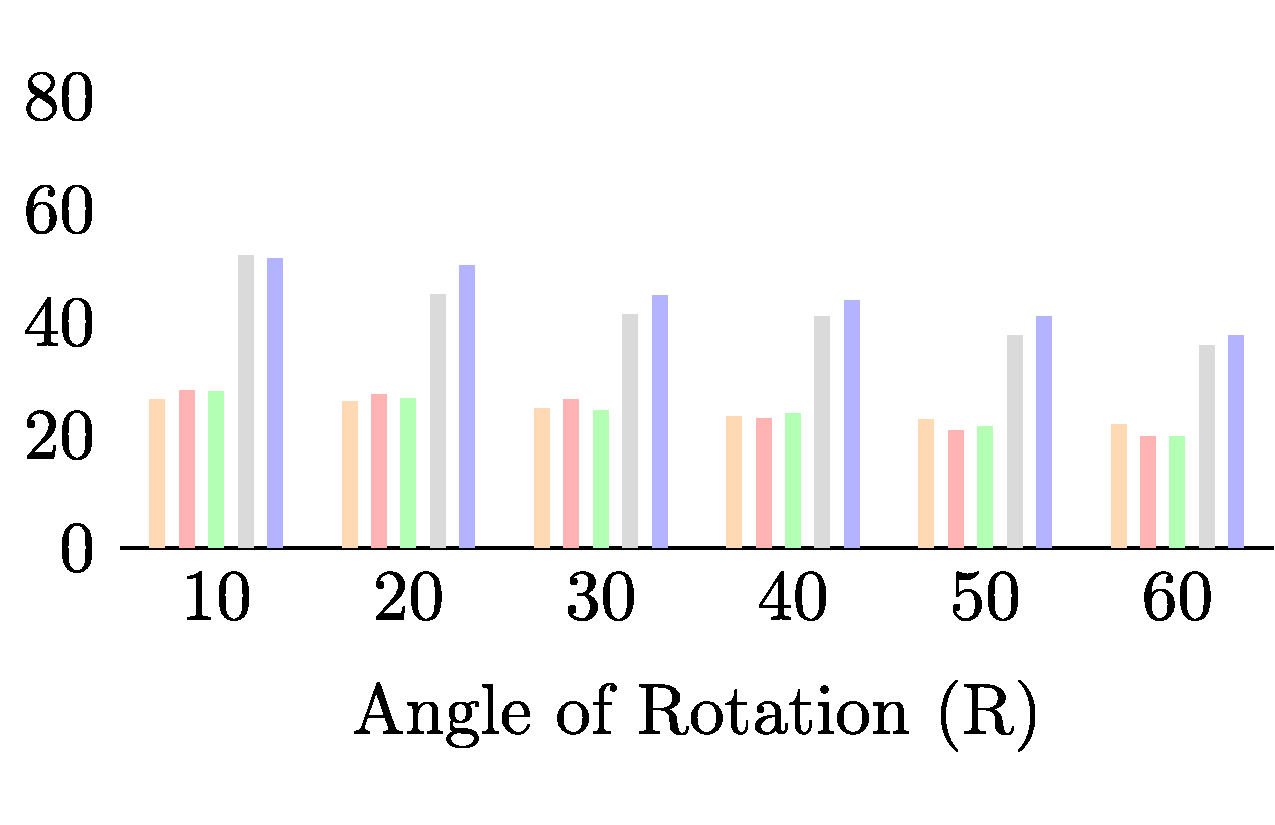
\includegraphics[width=0.45\linewidth]{agat/images/ablation_r.pdf}
        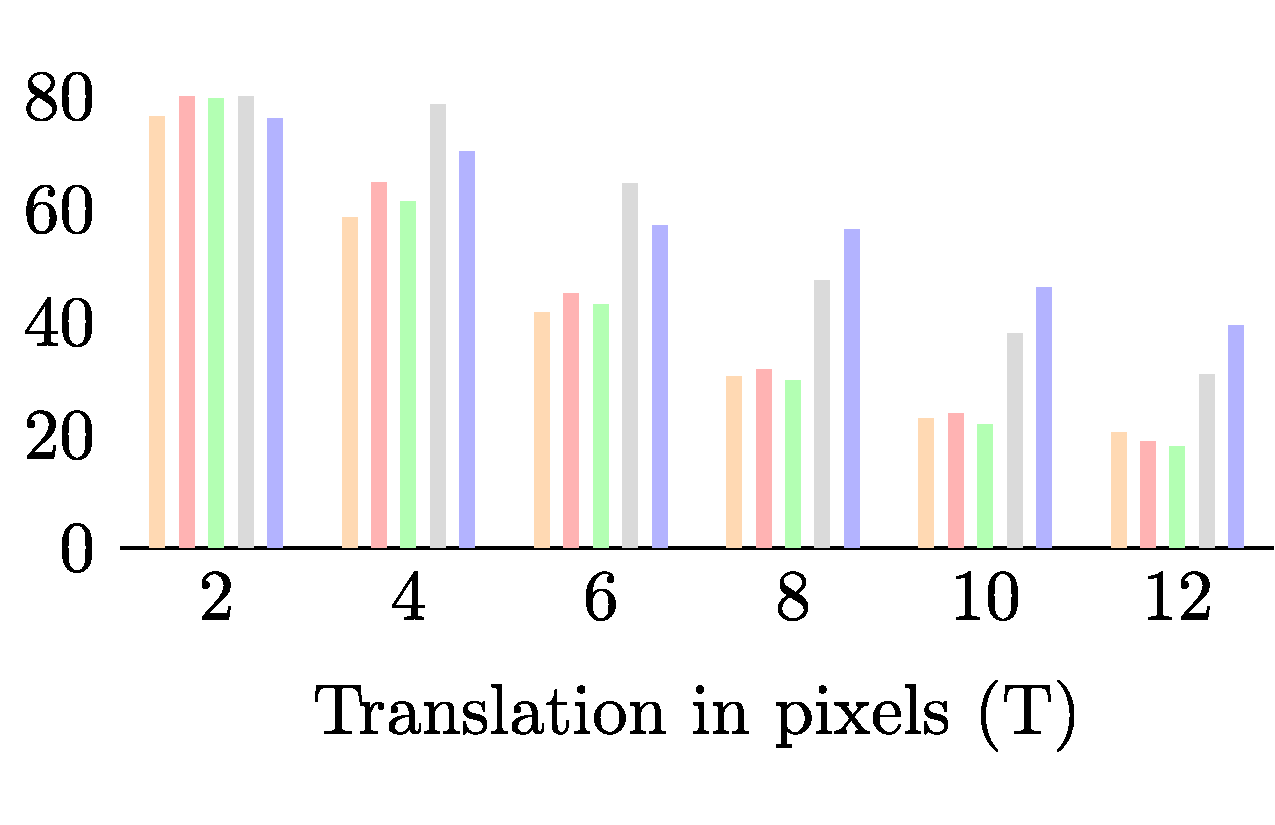
\includegraphics[width=0.45\linewidth]{agat/images/ablation_t.pdf}
        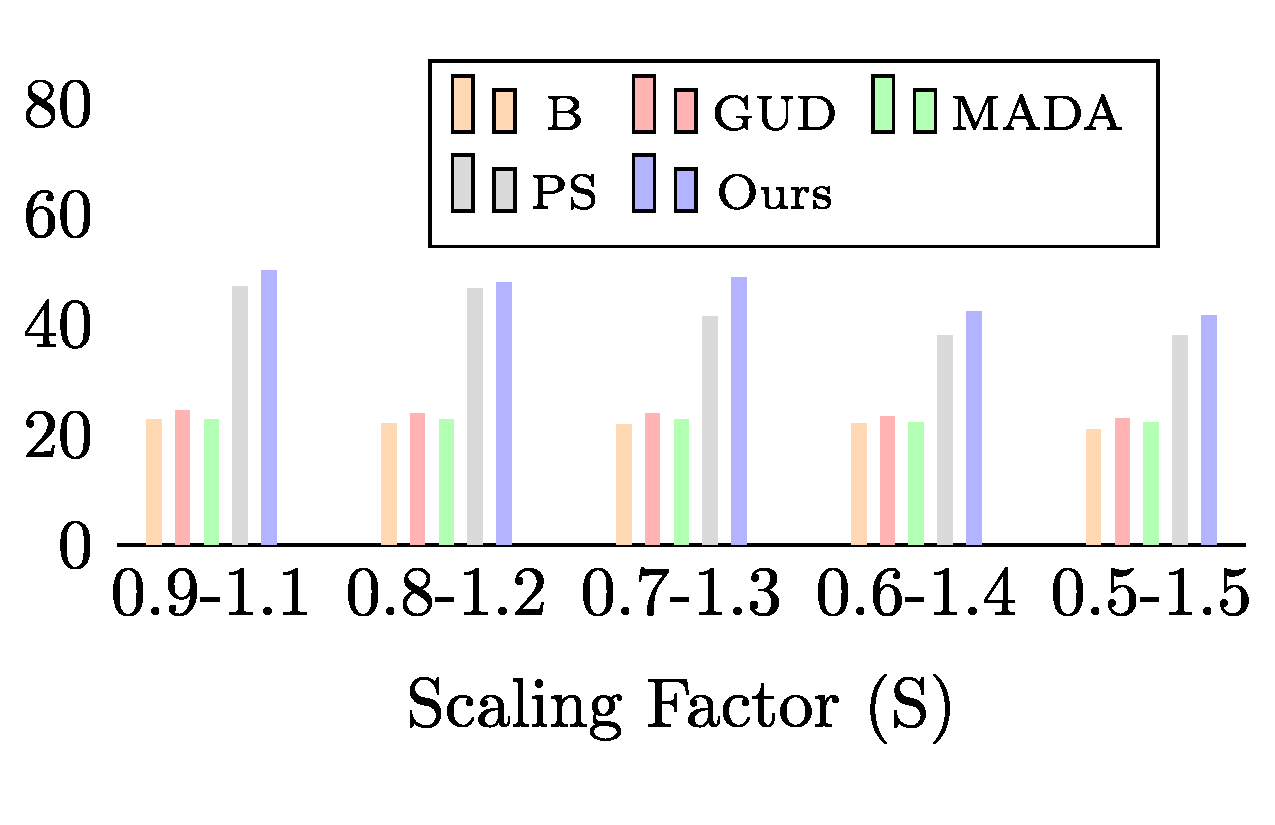
\includegraphics[width=0.45\linewidth]{agat/images/ablation_s.pdf}
        \caption{Comparison of random RTS accuracies when controlling each parameter to a max. value. Left: R, Center: T, Right: S}
    \end{figure*}
    \begin{table}
    \centering 
    % \small
    % \resizebox{0.7\linewidth}{!}{               
    \begin{tabular}{@{}cccccc@{}}
        \toprule
        $\mathbf{N_{aug}}$ & $\mathbf{T_{aug}}$ & \textbf{R} & \textbf{T} & \textbf{S} & \textbf{RTS} \\
        \toprule
        1 & 10 & 84.12 & 43.33 & 96.65 & 34.12 \\
         & 30 & 83.80 & 54.17 & 95.89 & 40.46 \\
         & 50 & 84.49 & 59.97 & 96.29 & 47.62 \\ 
         & 70 & 84.35 & 62.76 & 96.24 & 51.13 \\
        \midrule
        2 & 10 & 84.97 & 47.21 & 96.41 & 36.84 \\
         & 30 & 84.93 & 52.95 & 96.11 & 41.43 \\
         & 50 & 86.35 & 61.07 & 95.76 & 47.59 \\
         & 70 & 84.59 & 62.75 & 95.79 & 50.28\\
        \bottomrule
    \end{tabular}
    % }
    \caption{The effect of augmentation interval ($N_{aug}$) at different percentages of augmented samples 
    ($T_{aug}$). 
    }
    \label{}
\end{table}

\begin{table}
    \centering 
    % \small 
    % \resizebox{0.7\linewidth}{!}{               
    \begin{tabular}{@{}cccccc@{}}
        \toprule
        \textbf{Loss} & $\mathbf{T_{aug}}$ & \textbf{R} & \textbf{T} & \textbf{S} & \textbf{RTS} \\
        \toprule
        GT 
         & 10 & 85.41 & 29.48 & 96.74 & 23.57\\
         & 30 & 84.82 & 48.46 & 96.75 & 37.80\\
         & 50 & 84.17 & 52.44 & 95.86 & 41.82 \\
         & 70 & 84.07 & 55.14 & 95.70 & 44.20 \\
        \midrule
        GT~+~CR
         & 10 & 84.97 & 47.21 & 96.41 & 36.84 \\
         & 30 & 84.93 & 52.95 & 96.11 & 41.43 \\
         & 50 & 86.35 & 61.07 & 95.76 & 47.59 \\ 
         & 70 & 84.59 & 62.75 & 95.79 & 50.28 \\
        \bottomrule
    \end{tabular}
    % }
    \caption{
        The effect of classification loss function at different percentages of augmented samples. GT denotes the first term and CR is consistency regularization in Eq~\eqref{agat:eq:loss_distill}.
    }
    \label{tab:mnist_ablation}
\end{table}
    The pixel-level perturbation methods still perform reasonably well on rotation and scale experiments in Table~\ref{tab:mnist_geom} because in each case the rotations/translations/scale are randomly sampled, resulting in several test examples that are very close to the training examples (with no RTS). In order to resolve this further, we study the performance by controlling the magnitude of R, T, and S in the test set. Figure~\ref{fig:mnist_rts} shows the bar-plots when the range of rotation is varied from $(-10, 10)$ to $(-60, 60)$, translation from $(-2, 2)$ to $(-12, 12)$ pixels, and scaling factor from $(0.9, 1.1)$ to $(0.5, 1.5)$.
    It can be observed that at higher severity of perturbation, our model (in blue) significantly outperforms all baselines.
    The model trained with Perturbations Sets~\citep{wong2020learning} (in gray) is competitive at lower severities.

    We also analyze the effect of the number of augmented samples ($T_{aug}$) expressed as a percentage of the size of the training data, while controlling for the augmentation interval $N_{aug}$. As expected, larger number of augmented samples improve robustness even higher than in table \ref{tab:mnist_geom} (which fixes number of additional augmented examples at $30\%$ for all baselines). 
    Larger augmentation intervals contribute positively at lower percentages of augmented samples.
    
    Finally, we perform an ablation study with and without the consistency regularization defined in Eq~\eqref{agat:eq:loss_distill} and show that the regularization indeed helps improve performance.

%%%%%%%%%%%%%%%%%%%%%%%%%%%%%%%%%%%%%%%%
\subsection{Common Image Corruptions}
Image corruptions are another common class of perturbations. These can occur due to image digitization artifacts, weather, camera calibration, and other sources of noise.

    \paragraph{Dataset:}
    The CIFAR10 dataset~\citep{krizhevsky2009learning}
    contains $50k$ training images belonging to $10$ classes.
    Recently, CIFAR10-C~\citep{hendrycks2018benchmarking} which contains image corruptions for CIFAR10 images, was proposed to benchmark robustness of image classifiers, with 4 major and  15 fine-grained categories of corruption: \textit{Weather} (fog, snow, frost), \textit{Blur} (zoom, defocus, glass, motion), \textit{Noise} (shot, impulse, Gaussian), and \textit{Digital} (JPEG, pixelation, elastic transform, brightness, contrast).
    There are five levels of severity of corruptions; we focus on the highest severity.


    \paragraph{Surrogate Function:}
    We use a general surrogate function -- a composition of additive Gaussian noise and Gaussian blur filter parameterized by $\mathbf{\alpha} = \{\alpha_1, \alpha_2\}$:
    \begin{equation}
        \mathbf{x}^{gen} = \frac{1}{\sqrt{2\pi\alpha_1^2}}e^{-\frac{\mathbf{x}^2}{2\alpha_1^2}} + n \text{, ~where~ } n\sim \mathcal{N}(0, \mathbf{\alpha}_2).
    \end{equation}
    We evaluate the performance gains using this surrogate function with the proposed AGAT training on the challenging CIFAR-10-C dataset.

    \paragraph{Baselines:}
    Test-Time Training (TTT)~\citep{sun2020test} is a recent approach in which a classifier is trained only on source data, but the test sample is utilized to update the classifier during inference.
    Adversarial Logit Pairing (ALP)~\citep{kannan2018adversarial}, a technique for defending against adversarial attacks, and pixel-wise domain augmentation techniques MADA~\citep{qiao2020learning} and GUD~\citep{volpi2018generalizing} are also considered as baselines.
    We use ResNet-26~\citep{he2016deep} specially designed for CIFAR-10~\citep{russakovsky2015imagenet}, with group normalization~\citep{wu2018group} which is stable with different batch sizes.
    This acts as the naive classifier-only baseline (B).
    We also consider the classifier trained with an auxiliary self-supervised task of angle prediction~\citep{gidaris2018unsupervised} (B+SS).
    Our joint-training (JT) baseline is from TTT based on \citep{hendrycks2018benchmarking}.

    We compare three versions of our model: with additive noise only, with Gaussian filtering, and with a composition of Gaussian filter and noise. 
    Our models are trained for 150 epochs including pre-training epochs $N_{pre}\mathrm{=}100$, batch-size 128, and $M\mathrm{=}15$ update steps for adversarial augmentation.
    The number of augmented samples is $30\%$ of the original source data, and augmentation interval $N_{aug}$ is fixed at 2 epochs.
    For our model the coefficients in Equations~\ref{agat:eq:loss_constraint}, and~\ref{agat:eq:loss_distill} are: $\lambda_1=0.5, \lambda_2=0.5, \beta=0.25$.
    The learning rates $\eta, \mu$ for the classifier and adversarial augmentation are both 5e-5.

    \paragraph{Results:}
    \begin{table}
    \centering
    % \small
    % \resizebox{\linewidth}{!}{
    % \begin{tabularx}{\linewidth}{@{}l P{5.5mm}P{7.5mm}P{5.5mm}P{5.5mm}P{5.5mm}P{5.5mm}@{}}
    \begin{tabular}{l cccccc}
        \toprule 
        \textbf{Method} & \textbf{Src.} & \textbf{W} & \textbf{B} & \textbf{N} & \textbf{D} & \textbf{Avg.} \\
        \toprule 
        B       & 90.6 & 70.6 & 69.0 & 45.5 & 71.6 & 66.4\\
        B+SS    & 91.1 & 70.6 & 68.5 & 48.7 & 69.7 & 67.0\\
        GUD     & - & 71.7 & 59.2 & 30.5 & 64.7 & 58.3\\
        MADA    & - & 75.6 & 63.8 & 54.2 & 65.1 & 65.6\\
        JT      & 91.9 & 71.7 & 69.0 & 50.6 & 71.6 & 68.3\\
        ALP     & 83.5 & 60.9 & 74.7 & \textbf{75.4} & 68.5& 70.0\\
        TTT     & \textbf{92.1} & 73.7 & 71.3 & 54.2 & 73.4 & 70.5\\
        \midrule
        Ours (b. only) & \underline{91.3} & \underline{\textbf{78.4}} & \underline{\textbf{75.1}} & 49.3 & \underline{\textbf{75.4}} & 70.0\\
        Ours (n. only) & 90.3 & 75.0 & 73.3 & 62.4 & 73.1 & 71.3 \\
        Ours    & 89.3 & 77.8 & 74.1 & \underline{65.8} & 71.6 & \underline{\textbf{72.3}} \\
        \bottomrule
    \end{tabular}
    % }
    \caption{Comparison of classification accuracies on CIFAR-10-C corruption categories (Weather, Blur, Noise, Digital). Our best scores are underlined; overall best are bold.}
    \label{tab:cifar_cat}
\end{table}
    In Table~\ref{tab:cifar_cat} we show the classification accuracies on CIFAR10-C.
    It can be seen that our method consistently outperforms all baselines overall, and also on three of the four categories of corruptions (weather, blur, and digital).
    It is interesting to note that the ALP performance on the Noise category is distinctly greater than all previous methods, potentially because it is designed to defend against projected gradient descent adversarial attacks~\citep{madry2017towards}.
    ALP uses a similar loss function as Equation~\ref{agat:eq:loss_distill} to train the classifier, but still operates in pixel-space and does not perturb the attribute space.
    In Table~\ref{tab:cifar_cat} we also demonstrate that our models which uses only blur or only noise as surrogate are also better than previous state-of-the art. Note that the ``noise only'' model is in essence a pixel-level perturbation achieved by only perturbing along the variance parameter using AGAT training, and yet we see a significant boost in performance over all other pixel-level additive noise methods.
    Similarly, the ``blur only" model also gives performance boosts on weather and digital categories, further indicating the general applicability of our AGAT training approach.


\section{Discussion}
% \section{Conclusion}
% %%%%%%%%%%%%%%%%%%%%%%%%%%%%%%%%%%%%%%%%%%%%%%%%%%%%%%%%%%%%%%%%
% In this paper, we propose a new adversarial training strategy for robustness against large perturbations that are common in practical settings.
% Our adversarial training algorithm perturbs the attribute space to synthesize new images instead of pixel-level perturbations which are common to the robustness literature.
% The new CLEVR-Singles dataset that we have created can be used in future work for studying robustness to semantic shifts.
% We extensively evaluate AGAT training on three benchmarks and achieve state-of-the-art performance.
% We empirically show that AGAT is applicable to a three types of naturally occurring perturbations, and can be used with different classes of surrogate functions.
% AGAT can potentially be applied to a broad range of robustness problems not limited to classification.

% \section*{Acknowledgments} 
% This work was performed under the auspices of the U.S. Department of Energy by the Lawrence Livermore National Laboratory under Contract No. DE-AC52-07NA27344, Lawrence Livermore National Security, LLC. This document was prepared as an account of the work sponsored by an agency of the United States Government. Neither the United States Government nor Lawrence Livermore National Security, LLC, nor any of their employees makes any warranty, expressed or implied, or assumes any legal liability or responsibility for the accuracy, completeness, or usefulness of any information, apparatus, product, or process disclosed, or represents that its use would not infringe privately owned rights. Reference herein to any specific commercial product, process, or service by trade name, trademark, manufacturer, or otherwise does not necessarily constitute or imply its endorsement, recommendation, or favoring by the United States Government or Lawrence Livermore National Security, LLC. The views and opinions of the authors expressed herein do not necessarily state or reflect those of the United States Government or Lawrence Livermore National Security, LLC, and shall not be used for advertising or product endorsement purposes. This work was supported by LLNL Laboratory Directed Research and Development project 20-ER-014 and released with LLNL tracking number LLNL-JRNL-814425.

% \section*{Broader Impact}
% The concept of robustness is critical when it comes to deploying machine learning systems in practical settings where input signals may undergo perturbations due to weather (such as fog, smog, rain), digital corruptions in transmission, or changes in camera inclinations causing geometric transformations or artifacts such as defocusing, or motion blur.
% Our method for developing robust classifiers is broadly applicable if such classes of perturbations are known \textit{a priori}.

% Robustness research is also crucial for avoiding or removing unintended biases that may percolate from the training data into the classification model.
% Recent studies~\cite{bolukbasi2016man,zhao2017men,hendricks2018women} have shown that models trained on biased data can in fact amplify this bias when performing inference on test samples.
% We believe that work in the lines of AGAT could be potentially used for mitigating social biases due to biased training data, such as gender or racial biases.
\chapter{Adversarially Learned Transformations for Single-Source Domain Generalization}
\label{chap:alt}
In Chapter~\ref{chap:agat}, we looked at a relaxed setting of the generalization problem -- in that setting, information about the target domain was available in terms of a set of attributes that are known to differ at test time.
% (target samples are not available).
In this chapter we will go beyond attributes and address the harder and broader problem of domain generalization.

% As discussed earlier, domain generalization is the problem of making accurate predictions on previously unseen domains, especially when these domains are very different from the data distribution on which the model was trained. 
% In this chapter, we will tackle an even harder problem -- \textit{single source domain generalization (SSDG)}, where the model has access only to a single training domain, and is expected to generalize to multiple different testing domains. 
% This is especially hard because of the limited information available to train the model with just a single source. 

% \section{Introduction}
\begin{figure}
    \centering
    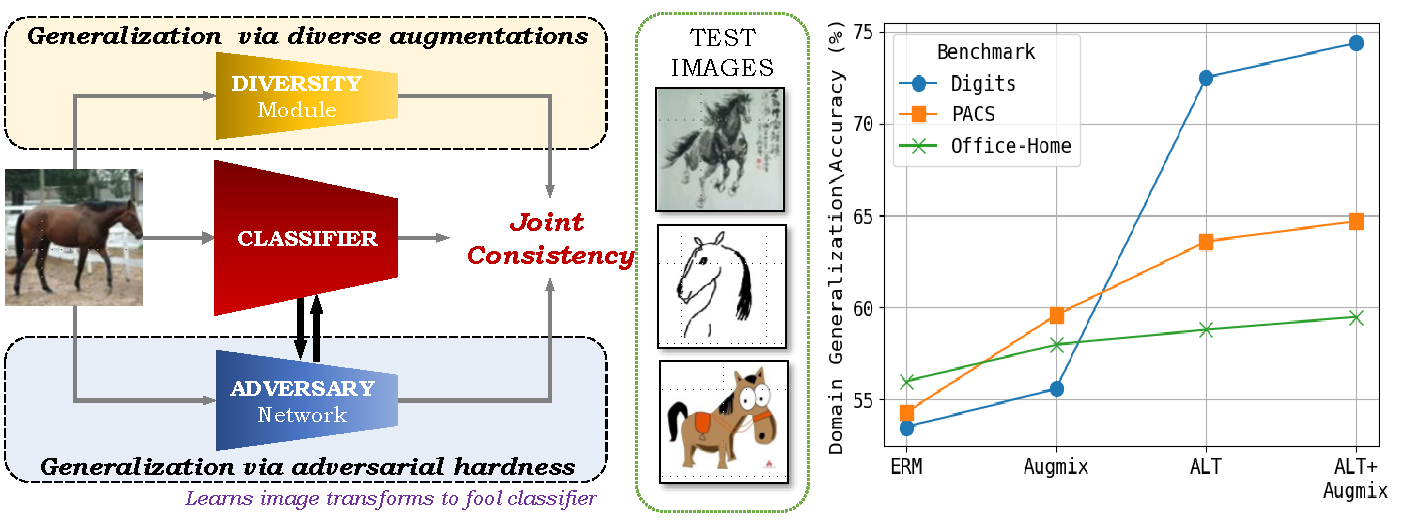
\includegraphics[width=\linewidth]{alt/figures/alt_teaser.pdf}
    \caption{
    This figure illustrates our approach which consists of a \textit{diversity} module (data augmentation functions such as Augmix~\citep{hendrycks2019augmix} or RandConv~\citep{xu2020robust}) and an \textit{adversary} network (ALT) (to learn image transformations that fool the classifier).
    We show an example from the PACS benchmark under the single-source domain generalization setting, with real photos (P) as the source domain and art paintings (A), cartoons (C), and sketches (S) as the target domains.
    The plot summarizes our results -- while diversity alone improves performance over the naive ERM baseline, adapting this diversity using adversarially learned transformations (ALT) provides a significant boost for domain generalization on multiple benchmarks.}
    \label{fig:alt_teaser}
\end{figure}


Domain generalization is the problem of making accurate predictions on previously unseen domains, especially when these domains are very different from the data distribution on which the model was trained. 
This is a challenging problem that has seen steady progress over the last few years \citep{carlucci2019domain,volpi2018generalizing,qiao2020learning,xu2020robust,nam2021reducing}. 
this chapter focuses on the special case -- single source domain generalization (SSDG) -- where the model has access only to a single training domain, and is expected to generalize to multiple different testing domains. 
This is especially hard because of the limited information available to train the model with just a single source. 

In the case where multiple training domains (i.e., multi-source DG) are available, recent analysis \citep{gulrajani2021in} shows that even simple methods like minimizing empirical risk jointly on all domains, performs better than most existing sophisticated formulations.
% on par with sophisticated formulations.
A corollary to this finding is that success in 
%SSDG
domain generalization is primarily dependent on \emph{diversity} -- i.e., exposing the model to as many potential training domains as possible.
As the SSDG problem allows access only to a single training domain, such an exposure must come in the form of diverse transformations of the source domain that can simulate the presence of multiple diverse domains ultimately leading to low generalization error. 
% which in this case must be in the form of diverse transformations of the source domain that can simulate the presence of multiple different domains ultimately leading to low generalization error. 

The idea of using diversity to train better models has been sufficiently explored -- many recent approaches have shown that a diverse set of augmentations during training improves a model's robustness under distribution shifts \citep{hendrycks2019augmix,yun2019cutmix,zhang2018mixup,cubuk2020randaugment}. 
However, the extent to which the model needs to be exposed to the diverse transformations is unclear, and over-exposure may hurt the model's generalization capabilities. 
Moreover, these methods define a strong prior in terms of the types of diversity that is desirable -- for e.g., in object recognition tasks, invariance to affine transformations, color jitter, blurs, or other kinds of pixel noise is desirable. 
Specific augmentations can be used if the type of diversity encountered at test time is known; for instance if it is known that the test set may contain random combinations of rotation, translation, and scaling, using augmentations that are correlated with this domain shift would lead good performance~\citep{gokhale2021attribute,benton2020learning,wong2020learning}.

Unfortunately, by design, these methods can only achieve invariance under small distribution shifts, like unknown corruptions, noise or imperceptible and perceptible adversarial attacks. 
These methods typically do not work effectively when the distribution shift is large and of a semantic nature, as in the case of domain generalization. 
On the other hand, some recent methods have directly used randomized convolutions to synthesize diverse image manipulations~\citep{xu2020robust}, motivated by the large space of potentially realizable functions induced by a convolutional layer, which cannot be easily emulated using simple analytical functions. 
 
In this chapter we hypothesize that, while diversity is critical in order to succeed in single domain generalization, diversity alone is insufficient. 
In other words, blindly exposing a model to a wide range of transformations cannot improve the generalization performance. Instead, we argue that other carefully designed forms of diversity are needed -- specifically those that can expose the model to unique, and task-dependent transformations with large semantic changes that are otherwise unrealizable with plug-and-play augmentations as before.  To this end, we introduce an adversary network whose objective is to find plausible image transformations that maximize classification error. We enforce a consistency between a \textbf{diversity module} and the \textbf{adversary network} during training along with the classifier's predictions. 

Our method, dubbed ALT (adversarially learned transformations), offers an interplay between diversity and adversity. Over time, a synergistic partnership between the diversity and adversary networks emerges, exposing the model to increasingly unique, challenging and semantically diverse examples that are ideally suited for single source domain generalization.  The adversary network benefits from the classifier being exposed to the diversity module, and as such avoid trivial adversarial samples with appropriate checks. This allows the adversarial maximization to explore a wider space of adversarial transformations that cannot be covered by prior work on pixel-level additive perturbations.
  
We demonstrate this advantage of our method empirically on multiple benchmarks -- PACS \citep{li2017deeper}, Office-Home \citep{venkateswara2017deep}, and Digits \citep{volpi2018generalizing}. On each benchmark, we outperform the state-of-the-art single source domain generalization methods by a significant margin.  Moreover, since our framework disentangles diversity and adversarial modules, we can combine it with various diversity enforcing techniques -- we identify two such state-of-the-art methods with AugMix \citep{hendrycks2019augmix}, and RandConv \citep{xu2020robust}, and show that placing them inside our framework leads to significantly improved generalization performance over their vanilla counterparts. 
We illustrate this idea in figure \ref{fig:alt_teaser} where we show an image of a horse from the 'photo' training distribution in PACS and the different styles of cartoon/sketch/art painting horses that may be encountered at test time. 

\paragraph{Contributions:}
We summarize our contributions below:
\begin{itemize}[nosep,noitemsep,leftmargin=*]
    \item We introduce a method, dubbed ALT, which produces adversarially learned image transformations that expose a classifier to a large space of image transformations for superior domain generalization performance. ALT performs adversarial training in the parameter space of an adversary network as opposed to pixel-level adversarial training.
    \item We show how ALT integrates diversity-inducing data augmentation and hardness-inducing adversarial training in a synergistic pipeline, leading to diverse transformations that cannot be realized by blind augmentation strategies or adversarial training methods on their own.
    \item We validate our methods empirically on three benchmarks demonstrating state-of-the-art performance, and provide insights into and analysis of approach.
\end{itemize}

% Instead, the model must be able to trade-off diversity and classifier performance as needed such that it achieves 'optimal' exposure in a given task, and no more --  which is challenging to define \emph{a priori}. Instead, we are able to achieve this trade-off using a consistency using an additional network that acts an adversary to the classifier by learning adversarial transformations of the input image for every single batch during training. By randomly initializing this network in each iteration, we ensure the adversarial transformations are unique, and diverse themselves. We then place a consistency objective between the diverse and adversarial transformations so together they expose the model to learn from both diverse and challenging domains
% \section{Related Work}
\textbf{Domain Generalization}
has been explored under both multi-source (MSDG) and single-source (SSDG) settings. Techniques designed for MSDG seek to utilize the multiple domains to perform feature fusion~\citep{shen2019situational}, learning domain-invariant features~\citep{ganin2016domain}, meta-learning~\citep{li2018learning}, invariant risk minimization~\citep{arjovsky2019invariant}, learning mappings between multiple training domains~\citep{robey2021model}, and style randomization~\citep{nam2021reducing}.
Gulrajani  \textit{et al.}~\citep{gulrajani2021in} provide an extensive comparative study of these approaches and report that simply performing ERM on the combination of source domains leads to the best performance. Many benchmarks have been proposed to evaluate MSDG performance such as PACS~\citep{li2017deeper}, OfficeHome~\citep{venkateswara2017deep}, Digits~\citep{volpi2018generalizing}, and WILDS~\citep{koh2021wilds} which is a compendium of MSDG datasets for various tasks such as image classification, text sentiment classification, text toxicity prediction, etc. In the context of multi-source DG, \citep{zhou2020learning} propose to synthesize novel domains using a conditional generator trained on multiple domains using cycle consistency -- whereas we are primarily interested in the single source setting where such a method may not be feasible. Moreover, we strictly synthesize novel domains as functions of the source domain, and place emphasis on the nature of functions that are learnable during training with a convolutional network with objectives such as an adversarial cost and consistency measures.

SSDG is a harder setting due to the lack of multiple datasets for using the above methods; most work in SSDG has therefore focused on data augmentation.
Notable among these methods is the idea of adversarial data augmentation -- ADA\citep{volpi2018generalizing} and M-ADA~\citep{qiao2020learning} apply pixel-level additive perturbations to the image in order to fool the classifier.  Resulting images are used as augmented data to train the classifier.
% is trained over the union of source dataset and adversarial samples.
RandConv~\citep{xu2020robust} shows that shape-preserving transformations in the form of random convolutions of images lead to impressive performance gains on Digits.
% benchmark.

\textbf{Robustness to Image Corruptions.}
There has also been interest in training classifiers that are robust to corruptions that occur in the real world, such as different types of noise and blur, artifacts due to compression techniques, and weather-related environments such as fog, rain, and snow.
\citep{vasiljevic2016examining,geirhos2018generalisation} show that training models with particular types of corruption augmentations does not guarantee robustness to other unseen types of corruptions or even different severities of corruptions. 
Hendrycks~ \textit{et al.}~\citep{hendrycks2018benchmarking} curate benchmarks (ImageNet-C and CIFAR-C) to test robustness along a fixed set of corruptions.
They also provide a benchmark called ImageNet-P which tests robustness against other corruption types such as small tilts and changes in brightness.
A similar benchmark for corruptions of handwritten digit images, MNIST-C~\citep{mu2019mnist} has also been introduced.

% \paragraph{Robustness to Adversarial Attacks}

\textbf{Data Augmentation}
has been an effective strategy for improving in-domain generalization using simple techniques such as random horizontal flips and cropping~\citep{he2016deep}, random occlusion or removal of patches~\citep{devries2017improved,zhong2020random}.
Data augmentation techniques have been shown to improve robustness against adversarial attacks and natural image corruptions~\citep{zhang2018mixup,yun2019cutmix,cubuk2020randaugment}.
Learning to augment data has been explored in the context of object detection~\citep{zoph2020learning} and image classification~\citep{ratner2017learning,cubuk2019autoaugment,zhang2019adversarial}. 
% - previous methods for SSDG: naive data aug, 

% - style changes, style normalization 

% - diversity: augmix, randconv, older random projection papers, 

% - adversarial data aug --- talk about how adv training can only provide resiliency to small perturbations 

%  - newer methods when some info is known about target (but no dataset available) -- agat, perturbation sets rts

\section{Proposed Approach} 
% \paragraph{Preliminaries.}
Under the single-source domain generalization setting, consider the training dataset $\mathcal{D}$ containing $N$ image-label pairs $\mathcal{D} = \{(\xx_i, \yy_i)\}_{i=1}^{N}$, and a classifier $f$ parameterized by neural network weights $\theta$. 
The standard expected risk minimization (ERM) approach seeks to learn $\theta$ by minimizing the the in-domain risk measured by a suitable loss function such as the binary cross-entropy loss.
\begin{equation}
    \mathcal{R}_{ERM} = \underset{\xx\in\mathcal{D}}{\E} \mathcal{L}_{BCE}(f(\xx;\theta), \yy).
    \label{alt:eq:erm}
\end{equation}
For SSDG, we are interested in a classifier that has the least risk on any \textit{unseen} target domain $\mathcal{D}^\prime$ that is not observed during training. Note that in SSDG, there is only domain shift and no label shift, i.e. we assume the same classes exist in the training and testing domains. 
Our approach builds on diversity based and adversarial augmentation approaches which we outline next. 

\paragraph{Generalization via Diversity.} A successful strategy to improve generalization error on unseen domains is to utilize a diverse set of pre-defined transformations, $\mathcal{F}_{div}$, to synthesize data augmentations that emphasize the invariance properties that are important for $f(\theta)$ to learn. Methods that fall under this category modify Equation \ref{alt:eq:erm} as follows: 
\begin{equation}
    \label{alt:eq:div_erm}
    \mathcal{R}_{div} = \underset{\xx\in\mathcal{D}}{\E} \mathcal{L}_{BCE}(f(\xx; \theta), \yy) + \lambda_{KL} D_{KL},
\end{equation}
where $D_{KL}$ is a consistency term, typically a divergence, such as KL-Divergence, between the softmax probabilities of the classifier obtained with the clean and transformed data, respectively, \textit{e.g.}, $D_{KL} = KL(f(\xx) ||f(\mathcal{F}_{div}(\xx)))$. 
When $\mathcal{F}_{div}$ is chosen as a set of pre-defined transformations like shear, rotate, color jitter etc., this approach is referred to as AugMix \citep{hendrycks2019augmix}, and when it is a set of randomly initialized convolutional layers this method becomes RandConv \citep{xu2020robust} -- both of which are among the most effective strategies to enforce diversity-based consistencies for generalization.
Although these methods have the advantage of being simple pre-defined transformations that are dataset agnostic, they suffer from drawbacks under the SSDG setting.
When executed on their own, they may not capture sufficient diversity in terms of \textbf{large} semantic shifts, such as when expecting generalization on sketches from a model trained on photos.
% However, these methods suffer from a few drawbacks -- they are pre-defined and capture a large class of potential image transformations (particularly rand-conv), but when executed on their own, they may not capture sufficient diversity in terms of \emph{large} semantic shifts. 

\paragraph{Generalization via adversarial hardness.}
An alternative approach to domain generalization is via adversarial augmentation  which exposes a classifier to `hard' samples during training -- defined broadly as examples that are carefully designed to cause the model to fail. Such samples are augmented to the training set, with the expectation that exposure to such adversarial examples can improve the model's generalization performance on unseen domains \citep{volpi2018generalizing,qiao2020learning}. This is commonly enforced by learning an additive noise vector which when added, maximizes classifier cost. Unfortunately in the case of domain generalization, these methods have failed to match the performance of diversity-only methods optimizing for the cost outlined in Equation~\ref{alt:eq:div_erm}. This is in part because they lack sufficient diversity, and by design they can only guarantee robustness to small perturbations from the training domain, as opposed to large semantic shifts, which are crucial for domain generalization.

% \begin{equation}
%     \label{alt:eq:div_erm}
%     \mathcal{R}_{adv} = \underset{||\delta||_p < \epsilon}{\textrm{max}}~\mathcal{L}_{BCE}(f(\xx+\delta;\phi); \theta), \yy)
% \end{equation}

\begin{algorithm}[t]
    \caption{Adaptive Diversity via ALT}
    \begin{algorithmic}[0]
        \State \textbf{Input:} Source dataset $\mathcal{D}=\{(\xx_i,\yy_i)\}_{i=1}^N$ 
        \State \textbf{Output:} Learned weights $\theta^*$  
    \end{algorithmic}
    \begin{algorithmic}[1]
        \State \textbf{Initialize:} $\theta\gets\theta_0$ \algorithmiccomment{weights of $f()$}
        \ForEach{$t \in \{1\dots T\}$}%
            \State $\xx_t, \yy_t \sim\mathcal{D}$ \algorithmiccomment{\textit{sample input batch}}
            % \Statex ~~\quad$\triangleright$~\textit{train on source only}
            \If{$t < T_{pre}$} 
                \State $\theta\gets\theta - \eta\nabla \mathcal{L}_{cls}(f(\xx_t;\theta), \yy_t))$ 
            % \Statex ~~\quad$\triangleright$~\textit{ALT}
            \Else
                \State $\rho\gets\rho_0,~\phi\gets\phi_0$\algorithmiccomment{weights of $r()$, $g()$}
                \ForEach{$i\in{1\dots m_{adv}}$}
                    % \State $\phi\sim KN()$ \algorithmiccomment{initialize $\phi$}
                    % \State $\hat{\yy}\gets f(\xx; \theta)$
                    % \State $\xx_g \gets g(\xx;\phi)$
                    \State $\hat{\yy_g} \gets f(g(\xx;\phi);\theta)$
                    % \State $L_{adv} \gets \mathcal{L}_{cls}(\hat{\yy_g}, \yy) - \mathcal{L}_{TV}(\xx_g)$
                    % \State $\phi\gets\phi+\nabla\mathcal{L}_{adv}$
                    \State $\phi\gets\phi+\nabla(\mathcal{L}_{cls}(\hat{\yy_g}, \yy) - \mathcal{L}_{TV}(\xx_g))$
                \EndForEach
                % \Statex ~~\quad~~\quad $\triangleright$ \textit{Consistency}
                % \State $p_c,~p_r,~p_g \gets f(\xx; \theta),~f(r(\xx); \theta),~f(g(\xx); \theta)$
                % \State $p_{mix}\gets (p_c + w_r p_r + (2-w_r)p_g)/3$
                % \State $\mathcal{L}_{KL}\gets\sum_{j\in\{c,r,g\}}D_{KL}(p_{mix}||p_j)$ 
                % \State $\theta\gets\theta-\eta_{adv}\nabla((1-\lambda_{KL})\mathcal{L}_{cls} + \lambda_{KL}\mathcal{L}_{KL})$
                \State $\theta\gets\theta-\eta_{adv}\nabla\mathcal{L}_{ALT}$ \algorithmiccomment{see Eq.\ref{alt:eq:L_KL},\ref{alt:eq:L_ALT}}
            \EndIf 
        \EndForEach
        \State\Return $\theta$
\end{algorithmic}
\label{algo}
\end{algorithm}



\paragraph{Adversarially Learned Transformations (ALT).}
While diversity-only methods have shown promise, they are limited in their ability to generalize to domains with large semantic shifts; on the  other hand, techniques based purely on adversarial hardness are theoretically well-motivated but do not match the performance of diversity-based methods. Instead, in this chapter, we propose a new approach that takes the best of these two approaches using an adversary network that is trained to create \emph{plausible} image transformations that fool the classifier. These manipulated images are then used during training as examples on which the image must learn invariance. Since these perturbations are parameterized as learnable weights of a neural network, the network is free to choose large, complex transformations without being restricted to additive noise as done in previous work~\citep{volpi2018generalizing}. Further, this network is randomly initialized for each batch, making the types of adversarial transformations discovered unique and diverse over the course of training.  
%
% With this goal in mind, we propose learning transformations of source images using an adversarially trained image-to-image transformation network 

Formally, the adversary network transforms the input image as $g\colon\R^{C\times H\times W}\rightarrow\R^{C\times H\times W}$, where $C$, $H$, $W$ are the number of channels, height, and width of input images.
$g$ is parameterized by a set of weights denoted by $\phi$. This network, dubbed ALT, forms the backbone of our method.  To train ALT, we setup an adversarial optimization problem with the goal of producing transformations, which when applied to the source domain, can fool the classifier $f$.
While existing efforts dealing with robustness to small corruptions use pixel-level and $\ell_p$ norm-bounded perturbations to fool the model, we find that this is not sufficient for domain generalization as such methods do not allow searching for adversarial samples with semantic changes.
Instead, we directly perform adversarial training in the space of $\phi$, i.e., the neural network weights of ALT. Given input images $\xx$, parameters $\phi$ are randomly initialized, and the corresponding adversarial samples $\xx_g$ are found as:
\begin{equation}
    \xx_g = \underset{\phi}{\textrm{max}}~\mathcal{L}_{BCE}(f(g(\xx;\phi); \theta), \yy) - \mathcal{L}_{TV}(g(\xx;\phi)). 
    \label{alt:eq:adv_max}
\end{equation}
The first term seeks to update $\phi$ so as to maximizes the classifier loss, while $\mathcal{L}_{TV}$ (total variation)~\citep{rudin1992nonlinear} acts as a smoothness regularization for the generated image $\xx_g = g(\xx;\phi)$. The maximization in Equation \ref{alt:eq:adv_max} is solved by performing $m_{adv}$ steps of gradient descent with learning rate $\eta_{adv}$. We note a few important aspects of ALT -- unlike existing methods that explicitly place an $\ell_p-$norm constraint on the adversarial perturbations, we control the strength of the adversarial examples by limiting the number of optimization steps taken by $g$ to maximize classification error. Next, since we randomly initialize $g$ for each batch, the network is reset to a random function. In fact, when the number of adversarial steps is set to 0, $g$ behaves similar to RandConv \citep{xu2020robust} since its only a set of convolutional layers, with additional non-linearity. Finally, in addition to limiting the number of adversarial steps, we place a simple total variation loss on the generated image to force smoothness in the output. This naturally suppresses high frequency noise-like artifacts and encourages realistic image transformations and prevents the network from learning trivial transformations  -- for e.g., only noise or removing semantic content entirely. 

\paragraph{Improving Diversity.}
The samples $\xx_g$ obtained by solving Equation~\ref{alt:eq:adv_max} represent hard adversarial images that can be leveraged by the model to generalize to domain shift. But it also lends itself to exploit other forms of na\"ive diversity achieved by methods like RandConv and AugMix.
% On the other hand, augmentations such as RandConv and Augmix produce images that represent predefined image transformations such as random scaling, cropping, affine transformations, color jitter and so on.
We represent these ``diversity modules'' as $r$, which produce outputs $\xx_r{=}r(\xx)$. Our method utilizes these samples in the training process by enforcing a consistency between the predictions of the classifier on the source image and its transformations from $r$ and $g$. By including the diversity module into the optimization process, the invariances inferred by the classifier lead to stronger and more diverse adversarial examples in future epochs. 
Eventually, a synergistic partnership emerges between the diversity module and the adversary network to produce a wide range of image transformations that are significantly different from the source domain.  

Let $p_c$, $p_r$, and $p_g$ denote the softmax prediction probabilities of classifier $f$ on $\xx$, $\xx_r$, and $\xx_g$, respectively. Then the consistency between these predictions can be computed using Kullback-Leibler divergence~\citep{kullback1951information} as:
\begin{equation}
    \mathcal{L}_{KL} = D_{KL}(p_{mix}||p_c) + w_r D_{KL}(p_{mix}||p_r) + (2-w_r) D_{KL}(p_{mix}||p_g), 
    \label{alt:eq:L_KL}
\end{equation}
% \begin{equation}
%     \mathcal{L}_{KL} = D_{KL}(p_{mix}||p_c) + w_r D_{KL}(p_{mix}||p_r) 
%     % \nonumber\\
%     + (2-w_r) D_{KL}(p_{mix}||p_g), 
%     \label{alt:eq:L_KL}
% \end{equation}
where $p_{mix}$ denotes the mixed prediction:
\begin{equation}
    p_{mix} = \frac{p_c + w_r p_r + (2-w_r)p_g}{3}.
    \label{alt:eq:p_mix}
\end{equation}
The weight $w_r\in[0,2]$ controls the relative contribution of diversity and adversity to the consistency loss; $w_r>1$ implies that consistency with the diversity module has more weight and $w_r<1$ implies that consistency with the adversary network has more weight.
In all our benchmark experiments, we use $w_r=1$, i.e., both diversity and adversary are given equal importance.

Our final loss function for training the classifier is given as the convex combination of classifier loss $\mathcal{L}_{cls}$ with the consistency $\mathcal{L}_{KL}$:
\begin{align}
    \mathcal{L}_{cls} &= \mathcal{L}_{BCE}(f(g(\xx); \theta), \yy), \label{alt:eq:L_cls}\\
    \mathcal{L}_{ALT} &= (1-\lambda_{KL})\mathcal{L}_{cls} + \lambda_{KL}\mathcal{L}_{KL}.
    \label{alt:eq:L_ALT}
\end{align}


\paragraph{Implementation.}
In practice, ALT is implemented using the pseudocode shown in Algorithm~\ref{algo}.
In our experiments, we use RandConv or AugMix as the diversity module $r$ and a fully-convolutional image-to-image network as the adversary network $g$.
$g$ has 5 convolutional layers with kernel size $3$ and LeakyReLU activation.
We train the classifier for a total of $T$ batch iterations of which $T_{pre}$ iterations are used for pre-training the classifier using standard ERM on only the source domain (with only $\mathcal{L}_{cls}$).
For iterations $t>T_{pre}$, for each batch, we randomly initialize the weights of both $r$ and $g$ with the ``Kaiming Normal'' strategy~\citep{he2016deep} as our starting point for producing diverse perturbations, and update $g$ using the adversarial cost in Equation~\eqref{alt:eq:adv_max}.
After $g$ is adversarially updated for the given batch, we use the combination of classifier loss and consistency in Equation~\eqref{alt:eq:L_ALT} to update model parameters $\theta$.



\section{Experiments}


We validate our approach in this section with extensive empirical analysis using three popularly used domain generalization benchmarks. We follow this up with a detailed analysis of the behavior of ALT and its constituent parts. 


\paragraph{Datasets.}
The SSDG setup is as follows: we train on a single dataset as the source domain, and evaluate its performance on unobserved target (or test) domains with no access to any data from them during training. We demonstrate the effectiveness of our approach using three popular domain generalization benchmark datasets which we describe next -- (a) \textit{Digits}, we use follow the setting from Volpi~ \textit{et al.}~\citep{volpi2018generalizing} and use 1000 images from MNIST~\citep{lecun1998mnist} as the source dataset, and USPS~\citep{denker1988neural}, SVHN~\citep{netzer2011reading}, MNIST-M and SYNTH~\citep{ganin2015unsupervised} as the target datasets; (b) \textit{PACS:} Our second benchmark is the PACS dataset~\citep{li2017deeper} which consists of images belonging to 7 classes from 4 domains (P: photo, A: art painting, C: cartoon, S: sketch); and finally (c) \textit{Office-Home:} Our third benchmark is OfficeHome~\citep{venkateswara2017deep}, which consists of images belonging to 65 classes from 4 domains (A: art, C: clipart, R: real, P: product). 
%In all of these cases, we train models on each individual domain, while testing on the remaining domains and report the average accuracy across all domains as the domain generalization performance of the benchmark, repeated over for 5 random seeds.

\paragraph{Evaluation.}
For all datasets, we train models on each individual domain, while testing on the remaining domains. We provide fine-grained results on each test set as well as the average domain generalization performance. Accuracy is reported as the mean over 5 repetitions of the experiment with random seeds. We compare with several state-of-the-art techniques on single source domain generalization and compare three variants of our methods: ALT$_{g-only}$ refers to the simplest form of our method that only uses the adversary network during training without an explicit diversity module $r$. ALT$_{RandConv}$ and ALT$_{AugMix}$ utilize RandConv and AugMix, respectively, as the diversity module, where the consistency is now placed 
% on three terms 
as explained in \eqref{alt:eq:L_KL}.
% We report the mean and standard deviation of performance for 5 repetitions,


\begin{table}[t]
    \centering
    % \small
    \resizebox{\linewidth}{!}{
    \begin{tabular}{@{}l lllll l @{}}
        \toprule
        \textbf{Method} & \textbf{MNIST-10K} & \textbf{MNIST-M} & \textbf{SVHN} & \textbf{USPS} & \textbf{SYNTH} & \textbf{Target Avg.} \\ % & \textbf{Digits Avg.} \\
        \midrule
        ERM                                 & 98.40 {\footnotesize$\pm$ 0.84} & 58.87 {\footnotesize$\pm$ 3.73 } & 33.41 {\footnotesize$\pm$ 5.28 } & 79.27 {\footnotesize$\pm$ 2.70 } & 42.43 {\footnotesize$\pm$ 5.46 } & 53.50 {\footnotesize$\pm$ 4.23 } \\
        % & 62.48 {\footnotesize$\pm$ }\\
        ADA~\citep{volpi2018generalizing}    &  N/A  & 60.41 & 35.51 & 77.26 & 45.32 & 54.62 \\ % & \\
        M-ADA~\citep{qiao2020learning}       & 99.30 & 67.94 & 42.55 & 78.53 & 48.95 & 59.49 \\ % & \\
        AugMix~\citep{hendrycks2019augmix}   & 98.53 {\footnotesize$\pm$ 0.18} & 53.36 {\footnotesize$\pm$ 1.59} & 25.96 {\footnotesize$\pm$ 0.80} & 96.12 {\footnotesize$\pm$ 0.72} & 42.90 {\footnotesize$\pm$ 0.60} & 54.59 {\footnotesize$\pm$ 0.50}\\
        RandConv~\citep{xu2020robust}        & 98.85 {\footnotesize$\pm$ 0.04 } & 87.76 {\footnotesize$\pm$ 0.83} &	57.62 {\footnotesize$\pm$ 2.09} & 83.36 {\footnotesize$\pm$	0.96} & 62.88 {\footnotesize$\pm$ 0.78} & 72.88 {\footnotesize$\pm$ 0.58} \\
        \midrule 
        ALT$_{g-only}$                      & 98.46 {\footnotesize$\pm$0.27} & 74.28 {\footnotesize$\pm$1.36} & 52.25 {\footnotesize$\pm$1.54} & 94.99 {\footnotesize$\pm$0.68} & 68.44 {\footnotesize$\pm$0.98} & 72.49{\footnotesize$\pm$ 0.87} \\
        ALT$_{RandConv}$                    & 98.46 {\footnotesize$\pm$ 0.25} & 76.90 {\footnotesize$\pm$ 1.42} & 53.78 {\footnotesize$\pm$ 1.97} & 95.40 {\footnotesize$\pm$ 0.72} & 69.40 {\footnotesize$\pm$ 1.07} & \textbf{73.87} {\footnotesize$\pm$ 1.03}\\
        ALT$_{AugMix}$                      & 98.55 {\footnotesize$\pm$ 0.11} & 75.98 {\footnotesize$\pm$ 0.59} & 55.01 {\footnotesize$\pm$ 1.34} & 96.17 {\footnotesize$\pm$ 0.45} & 69.93 {\footnotesize$\pm$ 2.17} & \textbf{74.38} {\footnotesize$\pm$ 0.86}\\
        \bottomrule
    \end{tabular}
    }
    \caption{Single-source domain generalization accuracy (\%) on digit classification, with MNIST-10K as source and MNIST-M, SVHN, USPS, and SYNTH as target domains. Performance reported over five repetitions. Note:ADA and M-ADA do not report standard deviation.}
    \label{tab:results_digits}
\end{table}
\subsection{Digits}
\paragraph{Baselines.}
Our baselines include a na\"ive ``source-only'' baseline which is trained using expected risk minimization (ERM) on the source dataset, M-ADA~\citep{qiao2020learning} -- an adversarial data augmentation method, and AugMix~\citep{hendrycks2019augmix} 
and RandConv~\citep{xu2020robust} which exploit diversity through consistency constraints.
We use DigitNet~\citep{volpi2018generalizing} as the model architecture for all models for a fair comparison.
All models are trained for $T{=}10000$ iterations, with batch-size of $32$, learning rate of $0.0001$, using the \texttt{Adam} optimizer.
For ALT, we set the consistency coefficient $\lambda_{KL}{=}0.75$, adversarial learning rate $\eta_{adv}{=}5e{-}6$, number of adversarial steps $m_{adv}{=}10$, and equal weight $w_r{=}1.0$ for diversity and adversary networks.

\paragraph{Results.}
Table~\ref{tab:results_digits} shows the comparison between our method and prior art on the Digits benchmark.
Previous pixel-level adversarial training approaches (ADA and M-ADA) offer only marginal improvements over the na\"ive ERM baseline. The results for diversity-promoting data augmentation methods are mixed -- while AugMix is only $1.09\%$ better than ERM, RandConv provides a significant boost. Interestingly, the base version of our approach, ALT$_{g-only}$, which is exclusively based on adversarial training, is significantly better than pixel-level adversarial training.
More importantly, it is also better than diversity method AugMix, while performing lower than RandConv by a small margin $-0.39\%$.
When we trained ALT with  adaptive diversity (ALT$_{RandConv}$ and ALT$_{AugMix}$), we achieved the best performance, beating previous state-of-the-art by $0.99\%$ and $1.50\%$ respectively.
The hardest target domains on this benchmark have been SVHN and SYNTH, both of which are obtained from real-world images of street signs or house number signs.
On the other hand, USPS is closely correlated with MNIST, both being black-and-white, centered images of handwritten digits, while MNIST-M is derived from MNIST but with different backgrounds. AugMix fares poorly on both real-world datasets, but is able to generalize well to MNIST-M and USPS. However ALT is able to use its adversary network in combination with AugMix, resulting in an overall improvement.

\begin{figure*}
    \centering
    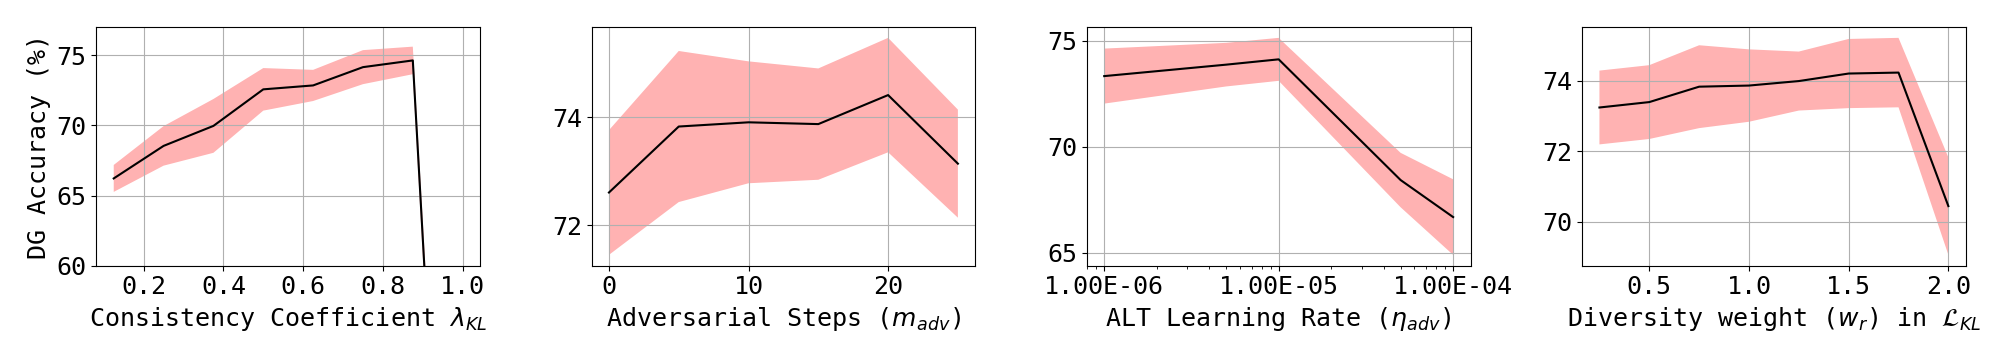
\includegraphics[width=\linewidth]{alt/figures/digits_hyperparam.png}
    \caption{\small{\textbf{Ablation Analysis:} We study the effect of each hyper-parameter in ALT on the average accuracy using the Digits benchmark. For each experiment we show 1 standard deviation around the mean over 5 runs. We observe that the consistency (left most) is generally important until a certain point, after which it becomes harmful; (left center) taking more adversarial steps improves performance; (right center) similarly, a small learning rate is preferred in training the adversary network, $g$, and performance degrades as the learning rate increases; (right most) Surprisingly, we find that the trade-off between diversity and ALT is non- trivial and dataset dependent.}}
    \label{fig:digits_hp}
\end{figure*}

\begin{table*}[t]
    \centering
    % \small
    \resizebox{\linewidth}{!}{
    \begin{tabular}{@{}l ccc ccc ccc ccc c@{}}
        \toprule
        \textbf{Method} & \textbf{A$\rightarrow$C} & \textbf{A$\rightarrow$S} & \textbf{A$\rightarrow$P} & \textbf{C$\rightarrow$A} & \textbf{C$\rightarrow$S} & \textbf{C$\rightarrow$P} & \textbf{S$\rightarrow$A} & \textbf{S$\rightarrow$C} & \textbf{S$\rightarrow$P} & \textbf{P$\rightarrow$A} & \textbf{P$\rightarrow$C} & \textbf{P$\rightarrow$S} & \textbf{Average}\\
        \midrule
        ERM                                 & 62.3 & 49.0 & 95.2 & 65.7 & 60.7 & 83.6 & 28.0 & 54.5 & 35.6 & 64.1 & 23.6 & 29.1 & 54.3\\
        JiGen~\citep{carlucci2019domain}     & 57.0 & 50.0 & 96.1 & 65.3 & 65.9 & 85.5 & 26.6 & 41.1 & 42.8 & 62.4 & 27.2 & 35.5 & 54.6\\
        ADA~\citep{volpi2018generalizing}    & 64.3 & 58.5 & 94.5 & 66.7 & 65.6 & 83.6 & 37.0 & 58.6 & 41.6 & 65.3 & 32.7 & 35.9 & 58.7 \\
        AugMix~\citep{hendrycks2019augmix}   & 68.4 & 54.6 & 95.2 & 74.3 & 66.7 & 87.3 & 40.0 & 57.4 & 46.8 & 67.3 & 26.8 & 41.4 & 59.6 \\
 
        RandConv~\citep{xu2020robust}        & 61.1 & 60.5 & 87.3 & 57.1 & 72.9 & 73.7 & 52.2 & 63.9 & 46.1 & 61.3 & 37.6 & 50.5 & 60.3\\
        SagNet~\citep{nam2021reducing}       & 67.1 & 56.8 & 95.7 & 72.1 & 69.2 & 85.7 & 41.1 & 62.9 & 46.2 & 69.8 & 35.1 & 40.7 & 61.9 \\
        \midrule 
        ALT$_{g-only}$                  & 63.5 & 63.8 &	94.9 & 68.9 & 74.4 & 84.6 & 39.7 & 61.1 & 49.3 &	68.8 & 43.4 & 50.8 & \textbf{63.6}\\
        ALT$_{RandConv}$                    & 63.6 & 65.8 & 92.5 & 69.1 & 75.1 & 84.5 & 40.1 & 61.7 & 50.8 & 68.4 & 43.4 & 55.2 & \textbf{64.2}\\
        ALT$_{AugMix}$                      & 65.7 & 68.2 & 93.2 & 71.9 & 74.2 & 86.0 & 40.2 & 62.9 & 49.1 & 68.5 & 43.5 & 53.3 & \textbf{64.7}\\
        % AugMax                            & 85.4 & 79.6 & 90.1 & 77.1 & 77.4 & 84.3 & 37.0 & 41.9 & 45.9 & 66.8 & 54.6 & 53.5 & 66.1 \\
        \bottomrule 
    \end{tabular}
    }
    \caption[SSDG PACS]{
        Single-source domain generalization accuracy (\%) on PACS~\citep{csurka2017domain}. 
        \textit{X$\rightarrow$Y} implies X is the source dataset and Y is the target dataset.
        \textit{P: photo; A: art-painting; C: cartoon; S: sketch.}
        Performance is reported as mean of 5 repetitions\footnotemark[1].
    }
    \label{tab:results_pacs}
\end{table*}


\subsection{PACS}
\footnotetext{$^*$standard deviation values are in the supplementary material.}
\paragraph{Baselines.}
Our baselines include JiGen~\citep{carlucci2019domain}, adversarial data augmentation (ADA)~\citep{volpi2018generalizing}, AugMix, RandConv, and SagNet~\citep{nam2021reducing} which is designed to reduce style bias using normalization techniques.
We use ResNet18~\citep{he2016deep} pre-trained on ImageNet as our model architecture and train all models for $2000$ iterations with batch-size of $32$, learning rate $0.004$, \texttt{SGD} optimizer with cosine annealing learning rate scheduler, weight decay of $0.0001$, and momentum $0.9$.
For ALT, we set consistency coefficient $\lambda_{KL}{=}0.75$, adversarial learning rate $\eta_{adv}{=}5e{-}5$, number of adversarial steps $m_{adv}{=}10$ and $w_r{=}1.0$.

\paragraph{Results.}
Results are shown in Table~\ref{tab:results_pacs}.
We observe that ALT without a diversity module (ALT$_{g-only}$) surpasses generalization performance of all prior methods including diversity methods RandConv and AugMix and the previous best SagNet~\citep{nam2021reducing}.
ALT with adaptive diversity further improves the results and ALT$_{AugMix}$ establishes a new state-of-the-art accuracy of $64.7\%$.
The most difficult target domains for previous methods has been \textit{Sketch (S)} since this is a set of rough human-drawn black-and-white sketches of real-life objects; the difficluty can be observed in terms of performance in columns $A{\rightarrow}S$, $C{\rightarrow}S$, and $P{\rightarrow}S$.
ALT significantly improves the performance on the sketch target domain, compared to the previous best.
ALT is also the best when generalizing from photos as the source to C,S,A as targets.
This is a very realistic setting since large-scale natural image datasets such as ImageNet~\citep{deng2009imagenet} are widely used and publicly available, while datasets for sketches, cartoons, and painting are not.

\begin{table*}[t]
    \centering
    % \small
    \resizebox{\linewidth}{!}{
    \begin{tabular}{@{}l ccc ccc ccc ccc c@{}}
        \toprule
        \textbf{Method} & \textbf{A$\rightarrow$C} & \textbf{A$\rightarrow$P} & \textbf{A$\rightarrow$R} & \textbf{C$\rightarrow$A} & \textbf{C$\rightarrow$P} & \textbf{C$\rightarrow$R} & \textbf{P$\rightarrow$A} & \textbf{P$\rightarrow$C} & \textbf{P$\rightarrow$R} & \textbf{R$\rightarrow$A} & \textbf{R$\rightarrow$C} & \textbf{R$\rightarrow$P} & \textbf{Average}\\
        \midrule
        ERM                                 & 42.61 & 59.18 & 69.45 & 48.37 & 56.09 & 59.38 & 46.07 & 40.18 & 68.19 & 63.12 & 45.13 & 74.34 & 56.00 \\
        AugMix~\citep{hendrycks2019augmix}   & 45.31 & 61.88 & 71.88 & 49.30 & 58.93 & 62.24 & 50.04 & 42.59 & 71.51 & 64.10 & 47.56 & 75.95 & 58.44 \\
        RandConv~\citep{xu2020robust}    & 43.98 & 55.28 & 67.31 & 45.49 & 56.58 & 59.03 & 43.80 & 43.19 & 66.50 & 57.62 & 48.26 & 72.97 & 55.00\\
        SagNet~\citep{nam2021reducing}   & 42.18 & 56.03 & 67.34 & 46.68 & 53.89 & 57.88 & 45.49 & 40.09 & 67.11 & 61.39 & 48.32 & 72.79 & 54.93\\
        \midrule 
        ALT$_{g-only}$                  & 47.26 & 61.14 & 71.21 & 48.88	& 57.81 & 60.99	& 48.15 & 46.70 & 69.30 & 64.85 & 52.84 & 76.28 & \textbf{58.78} \\
        ALT$_{RandConv}$                & 48.33 & 61.19 & 71.75 & 50.13 & 58.82 & 62.26 & 49.21 & 47.03 & 70.53 & 64.88 & 53.10 & 76.07 & \textbf{59.44}\\
        ALT$_{AugMix}$                  & 48.06 & 61.16 & 71.12 & 50.43 & 58.84 & 61.84 & 49.32 & 47.55 & 70.64 & 64.86 & 53.27 & 76.29 & \textbf{59.45} \\
        \bottomrule 
    \end{tabular}
    }
    \caption[SSDG Office-Home]{Single-source domain generalization accuracy (\%) on Office-Home~\citep{venkateswara2017deep} 
    % with mean and standard deviation 
    over five repetitions. 
    \textit{X$\rightarrow$Y} implies X is the source dataset and Y is the target dataset.
    \textit{R: real; A: art; C: clipart; P: product.}
    Performance is reported as mean of 5 repetitions\footnotemark[1].
    % ; detailed results with standard deviation values are in the supplementary material.
    }
    \label{tab:results_officehome}
\end{table*}
\subsection{Office-Home}
\paragraph{Baselines.}
For PACS, we follow the protocol from the previous state-of-the-art Sagnet~\citep{nam2021reducing} and use ResNet50 as the model architecture.
% and identical training settings and hyperparameters as PACS.
Note that we do not perform any hyperparameter tuning for OfficeHome and directly apply identical training settings and hyperparameters from PACS.

\paragraph{Results.}
Table~\ref{tab:results_officehome} shows the results on Office-Home.
We observe that RandConv (previous best on Digits) and SagNet (previous best on PACS) perform worse than ERM on OfficeHome, while AugMix is better by $2.44\%$.
All three variants of ALT surpass prior results, with ALT$_{AugMix}$ resulting in the best accuracy of $59.45\%$.
The most difficult target domain for previous methods are \textit{Art (A)} and \textit{Clipart (C)}, possibly because both sets have images with white backgrounds, while real world photos (R) and product images are naturally occurring.
ALT improves performance in each case when with A or C as target domain.
An observation similar to PACS can also be made here -- ALT is the best model under the realistic setting of generalizing from widely available real photos (R) to other domains.

\section{Analysis of ALT}
In this section we study the various components of ALT, and provide insights into their impact on generalization. 
\begin{figure*}
    \centering
    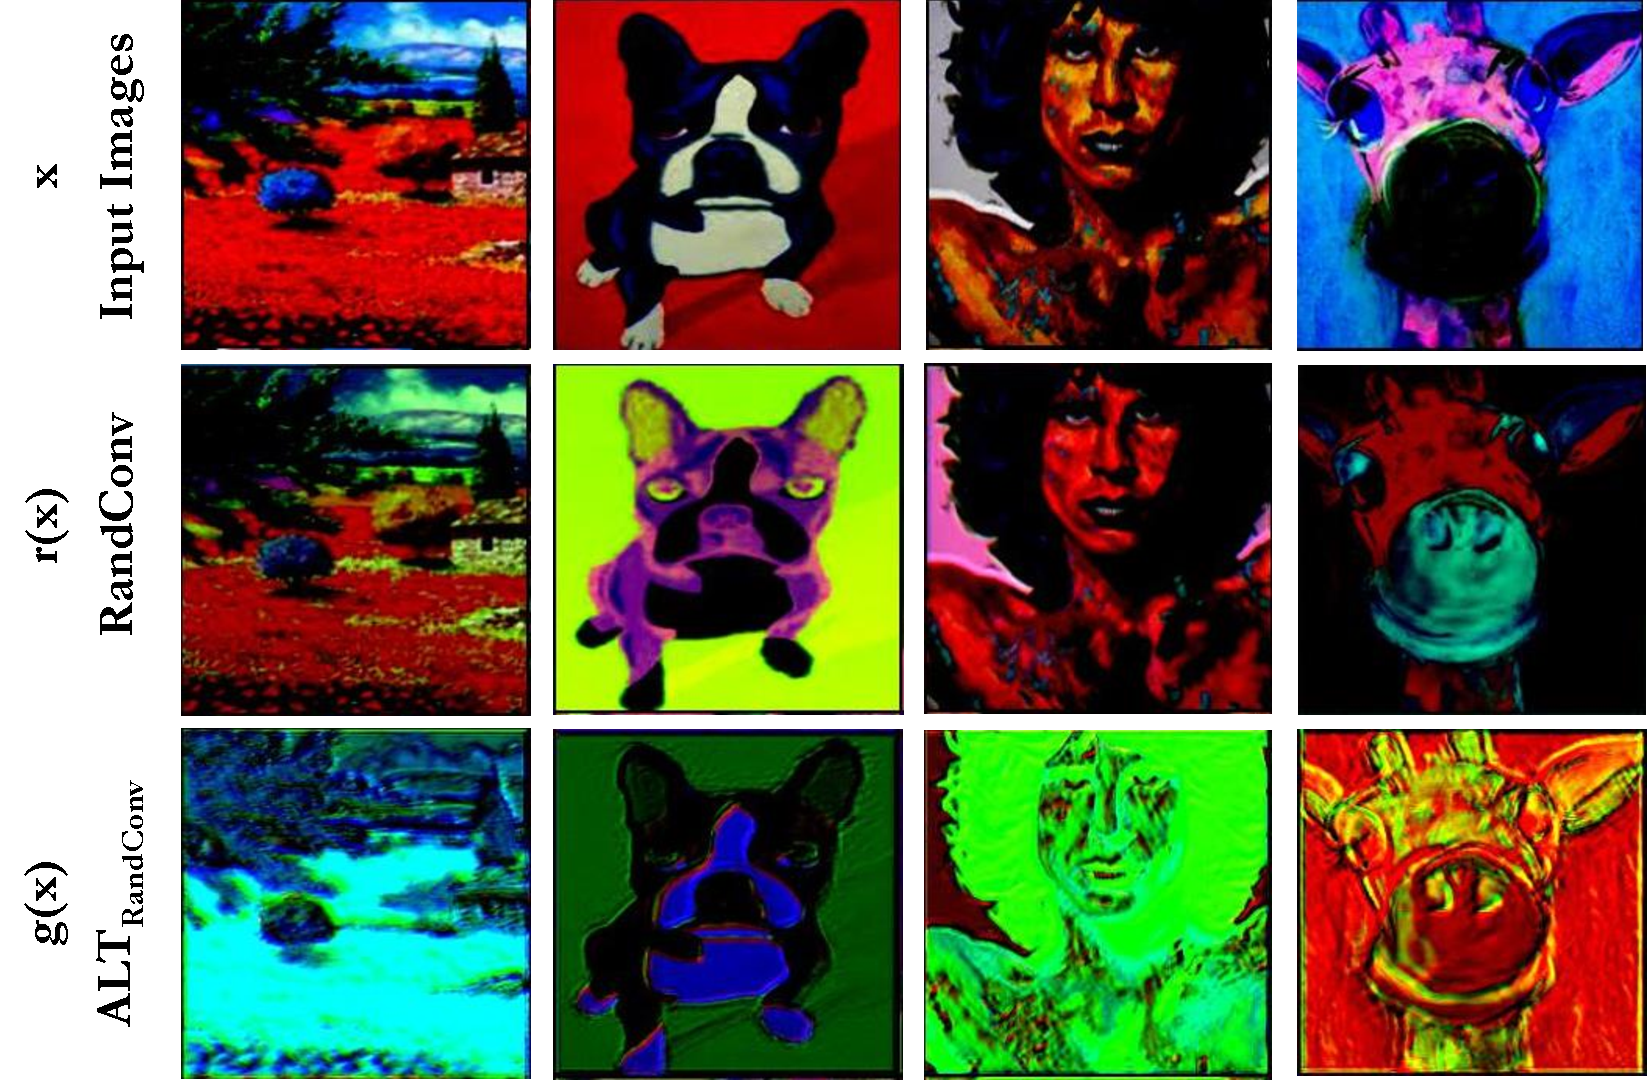
\includegraphics[width=0.48\linewidth]{alt/figures/viz_randconv_alt.pdf}
    \quad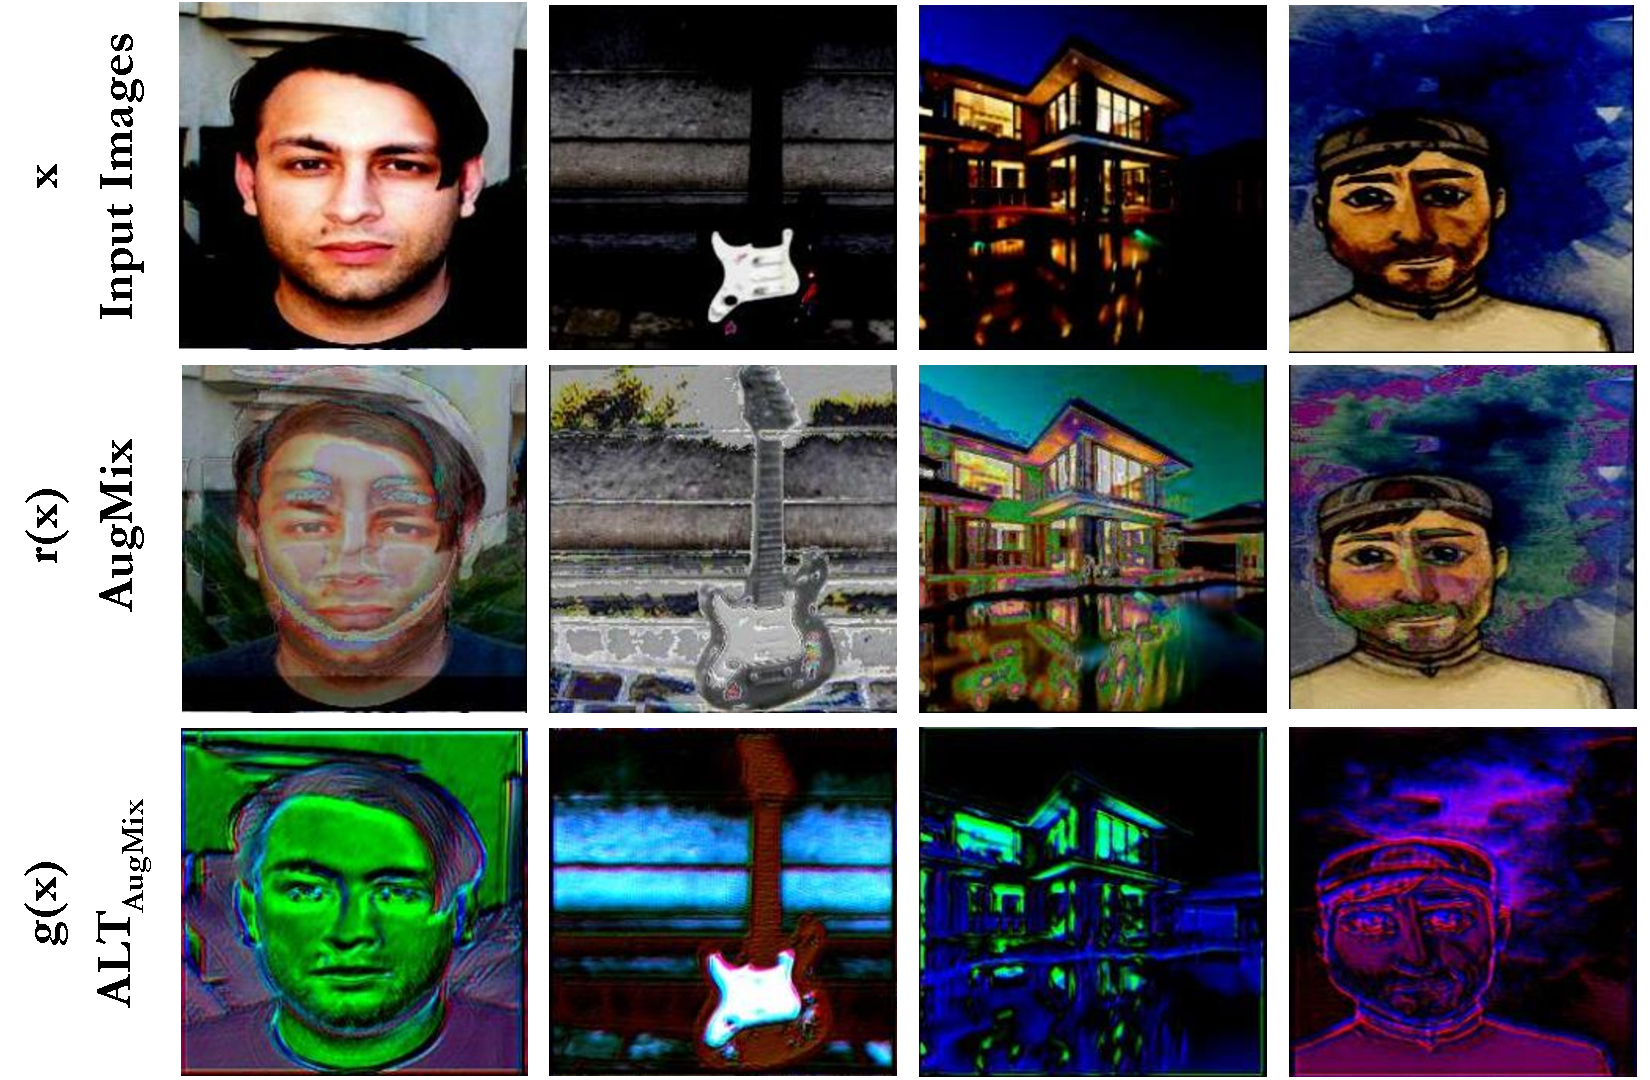
\includegraphics[width=0.48\linewidth]{alt/figures/viz_augmix_alt.pdf}
    \caption{Comparison of images transformed by data augmentation techniques RandConv \textit{(left)} and AugMix \textit{(right)} and their combination with ALT (ALT$_{RandConv}$ and ALT$_{AugMix}$), 
    illustrating the wide range of transformations learned by ALT.}
    \label{fig:viz_augs}
\end{figure*}

\paragraph{ALT is better than na\"ive diversity} Our first big insight is that ALT without an explicit diversity module still outperforms all the top performing methods across the benchmarks we evaluated on, indicating that learned adversarial transformations are a powerful way to train classifiers for generalization. They include diversity (achieved through random initializations) and adversarial images that help expose the classifier to large distribution shifts. Our next observation is that ALT makes the choice of diversity module fairly arbitrary. We see this effect on multiple benchmarks -- for example, on the Digits benchmark shown in  \Cref{tab:results_digits}, AugMix has a relatively poor generalization performance when compared with the baseline ERM whereas ALT$_{Augmix}$ achieves state of the art. This is again seen in the Office-Home benchmark shown in \Cref{tab:results_officehome}, where RandConv is worse than ERM, but ALT$_{RandConv}$ is the best performing method. We show examples of the image transformations learned with ALT in Figure~\ref{fig:viz_augs}, and it is clear that ALT achieves far more diverse and larger transformations of the input images than either AugMix or RandConv.

% - basically talk about diversity alone (Augmix/RC) -- see some boost, but varying results on each benchmark.
% MNIST -- augmix boosts by 1\% barely, but big jump for RandConv.
% On PACS and OfficeHome, AugMix is better than RandConv.
% - ALT without diversity is better than Diversity alone
% - ALT can better adapt its diversity when combined with RandConv and Augmix -- the combination and interplay between the adversarial cost and consistency, is key.


\paragraph{ALT Hyperparameters.}
The four main hyper-parameters that control ALT are: the consistency coefficient $\lambda_{KL}$ in Equation~\ref{alt:eq:L_KL} which decides the proportion between the classifier loss and KL-divergence consistency between transformations, 
number of adversarial steps and learning rate in the adversarial maximization of Equation~\ref{alt:eq:adv_max}, and the diversity weight $w_r$ which controls the interaction between the diversity module $r()$ and the adversary network $g()$ in Equation~\ref{alt:eq:p_mix}.
We investigate the effect of each of these on domain generalization accuracy in Figure~\ref{fig:digits_hp}.
The first plot shows that the consistency coefficient $\lambda_{KL}$ is impactful and a higher value leads to better generalization.
However at $\lambda_{KL}=1.0$ the accuracy degenerates to random performance; this is expected as the classifier loss gets $1-\lambda_{KL}{=}0$ weight.
From the second and third plots, we observe that an optimal value exists around 20 adversarial steps and learning rate of $1e{-}5$.
There is a fast drop in generalization at higher learning rates.
Increasing the diversity weight also leads to increase in generalization, however at $w_r{=}2$ the performance drops and corresponds to "diversity only" settings.
Clearly, the adversarial component is a critical factor that causes improvements in generalization.

\begin{table}[t]
    \centering
    % \small
    \begin{tabular}{@{}lccc@{}}
        \toprule
        \textbf{Architecture} & \textbf{Digits Average} & \textbf{PACS Average} \\
        \midrule
        FCN (2 layers) & 72.75 & 63.40 \\
        FCN (3 layers) & 73.74 & 63.92\\
        FCN (4 layers) & 74.10 & 64.41 \\
        FCN (5 layers) & 73.87 & 64.20 \\
        FCN (6 layers) & 74.15 & 63.78\\
        % ResNetGen-6~\cite{johnson2016perceptual} & \\
        % UNet-10~\cite{ronneberger2015u} & \\
        \bottomrule
    \end{tabular}
    \caption{Effect of the architecture of the adversity network $g$ on average domain generalization on the PACS and Digits benchmarks.}
    \label{tab:gvars}
\end{table}

% \begin{table}[t]
%     \centering
%     \begin{tabular}{cc}
%         \toprule
%         \textbf{Method}     & \textbf{DG Avg.}\\
%         \midrule
%         RandConv            & \\
%         AugMix              & 59.56\\
%         ALT$_{RandConv}$    & \\
%         ALT$_{AugMix}$      & \\
%         ALT$_{none}$        & \\
%         \bottomrule
%     \end{tabular}
%     \caption{PACS DG Average}
%     \label{tab:ablation_hd}
% \end{table}

\paragraph{Complexity of Adversary Network.}
In our experiments on the benchmark datasets we have used a simple fully convolutional network (FCN) with 5 convolutional layers.
We conduct additional analysis to understand how this choice affects generalization performance, and compare performance when using between 2 and 6 convolutional layers.
% We compare FCN with number of layers between 2 and 6.
% and two additional architectures -- U-Net-10~\citep{ronneberger2015u} with 5 downsampling and 5 upsampling operations (UNet-10) and a ResNet based generator (ResNetGen-6) with 3 downsampling and 3 upsampling operations. operations~\citep{johnson2016perceptual}.
% Note that the UNet and ResNet generators are considerably more sophisticated than FCN, and contain bottleneck architectures and skip connections.
We reuse all other training settings from our benchmark model $ALT_{RandConv}$ on both Digits and PACS.
For PACS, we observe that all ALT models compared are better than previous baselines including AugMix and RandConv.
For Digits, we observe that performance of ALT with a 2-layer $g$ is close to RandConv, and is greater than all previous baselines for higher depth of the network.
Increasing the number of layers, i.e., increasing the complexity of the adversary network leads to better performance upto 5 layers, even with the same learning rate.

% \paragraph{Qualitative Comparison of Diverse Augmentations}

% \begin{figure}[t]
%     \centering
%     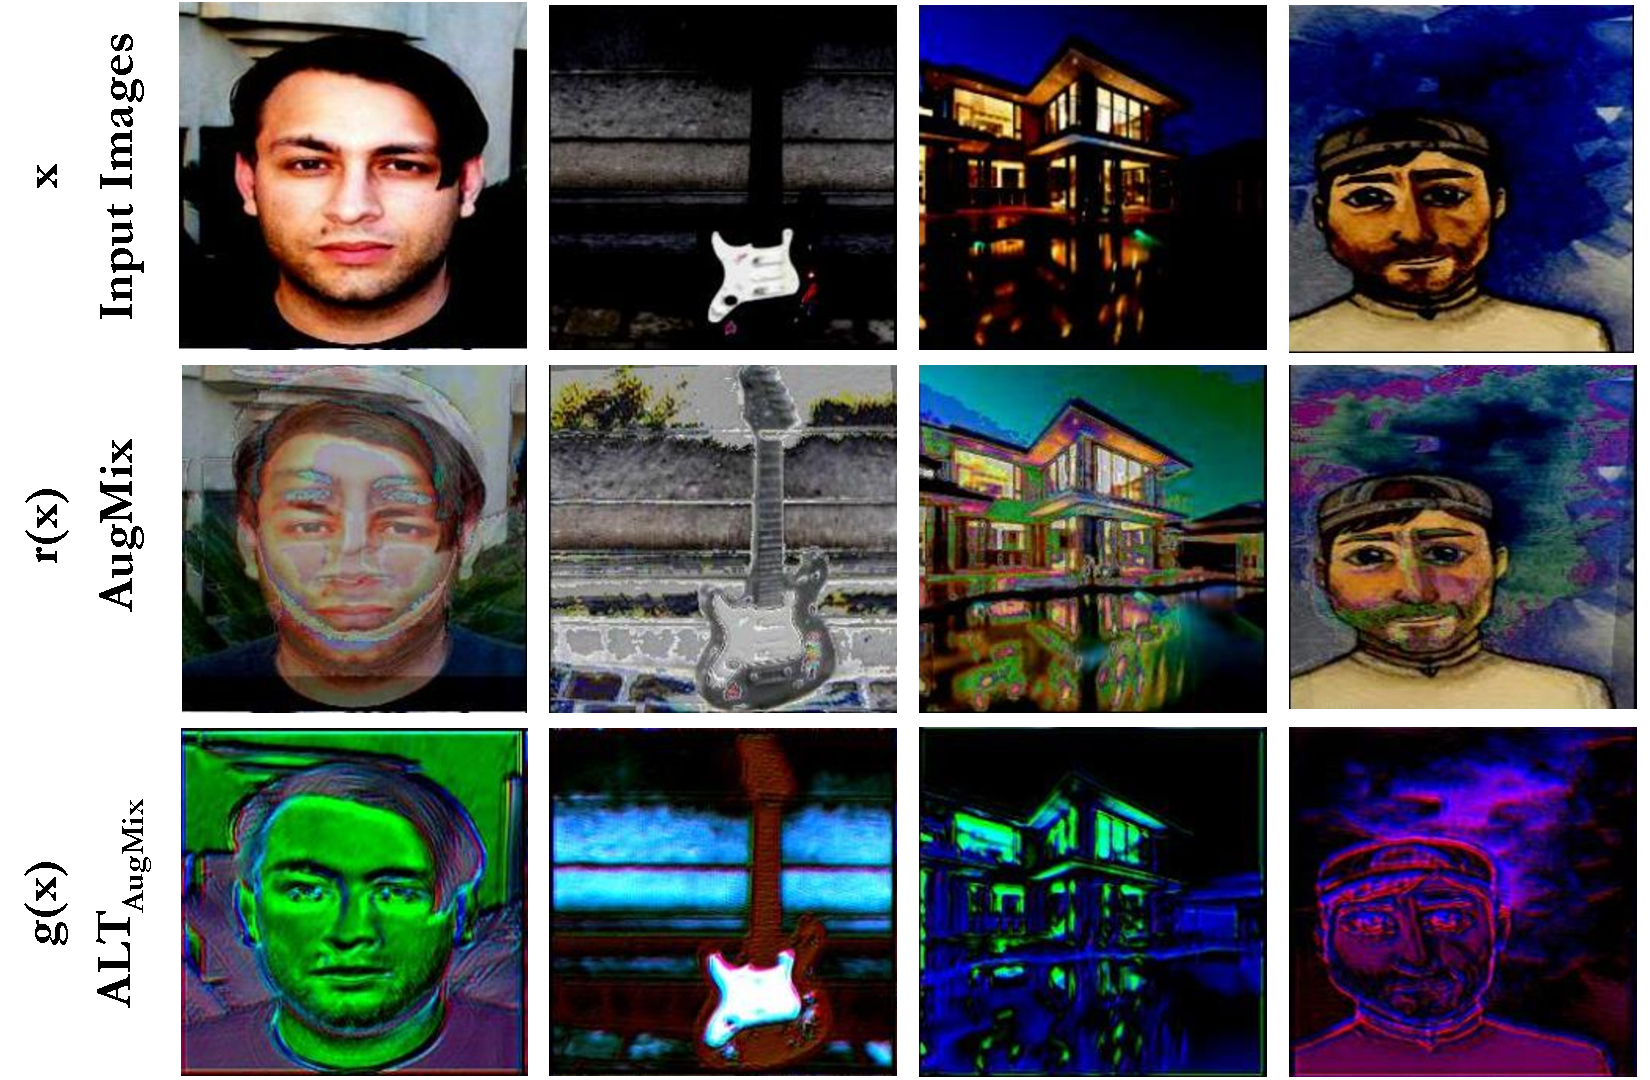
\includegraphics[width=\linewidth]{alt/figures/viz_augmix_alt.pdf}
%     \caption{Comparison of transformed images for AugMix and ALT$_{AugMix}$.}
%     \label{fig:viz_augmix}
% \end{figure}
% In Figure~\ref{fig:viz_augs} we illustrate the difference between the augmentations generated by RandConv, AugMix, ALT$_{g-only}$, ALT$_{RandConv}$ and ALT$_{AugMix}$.


\section{Conclusion}
In this paper, we address the problem of single source domain generalization. Our approach, Adversarially Learned Transformations (ALT) uses a randomly initialized convolutional network to learn plausible image transformations of the source domain that can fool the classifier. These images are used to enforce a consistency with the predictions on clean images. We showed that this strategy outperforms all existing techniques on multiple benchmarks because it is able to generate a diverse set of large transformations of the source domain. 
%
% In this paper, we started with the hypothesis that diversity alone or adversarial training alone is not enough for generalizing to unseen domains in the single-source domain generalization setting, as was confirmed by our experiments and mixed results on prior methods on different benchmarks.
We also find that ALT can be naturally combined with existing diversity modules like RandConv or AugMix to improve their performance (sometimes significantly). We also studied the different parts of ALT through extensive ablations and analysis to obtain insights into its performance gains. Our studies indicate that na\"ive diversity alone is insufficient, but needs to be combined adversarial transformations to maximize generalization performance. 



\chapter{Vision, Language, and Logic: Robustness to Logical Compositions}
\label{chap:vqalol}

%%%%%%%%%%%%%%%%%%%%%%%%%%%%%%%%%%%%%%%%%%%%%%%%%%%%%%%%%%%%%%%%
% \begin{abstract}
%%%%%%%%%%%%%%%%%%%%%%%%%%%%%%%%%%%%%%%%%%%%%%%%%%%%%%%%%%%%%%%%
Logical connectives and their implications on the meaning of a natural language sentence are a fundamental aspect of understanding.
In this paper, we investigate whether visual question answering (VQA) systems trained to answer a question about an image, are able to answer the logical composition of multiple such questions.
When put under this \textit{Lens of Logic}, state-of-the-art VQA models have difficulty in correctly answering these logically composed questions.
We construct an augmentation of the VQA dataset as a benchmark, with questions containing logical compositions and linguistic transformations (negation, disjunction, conjunction, and antonyms).
We propose our {Lens of Logic (LOL)} model which uses question-attention and logic-attention to understand logical connectives in the question, and a novel Fréchet-Compatibility Loss, which ensures that the answers of the component questions and the composed question are consistent with the inferred logical operation.
Our model shows substantial improvement in learning logical compositions while retaining performance on VQA.
We suggest this work as a move towards robustness by embedding logical connectives in visual understanding.
% \end{abstract}

\begin{figure}
    \centering
    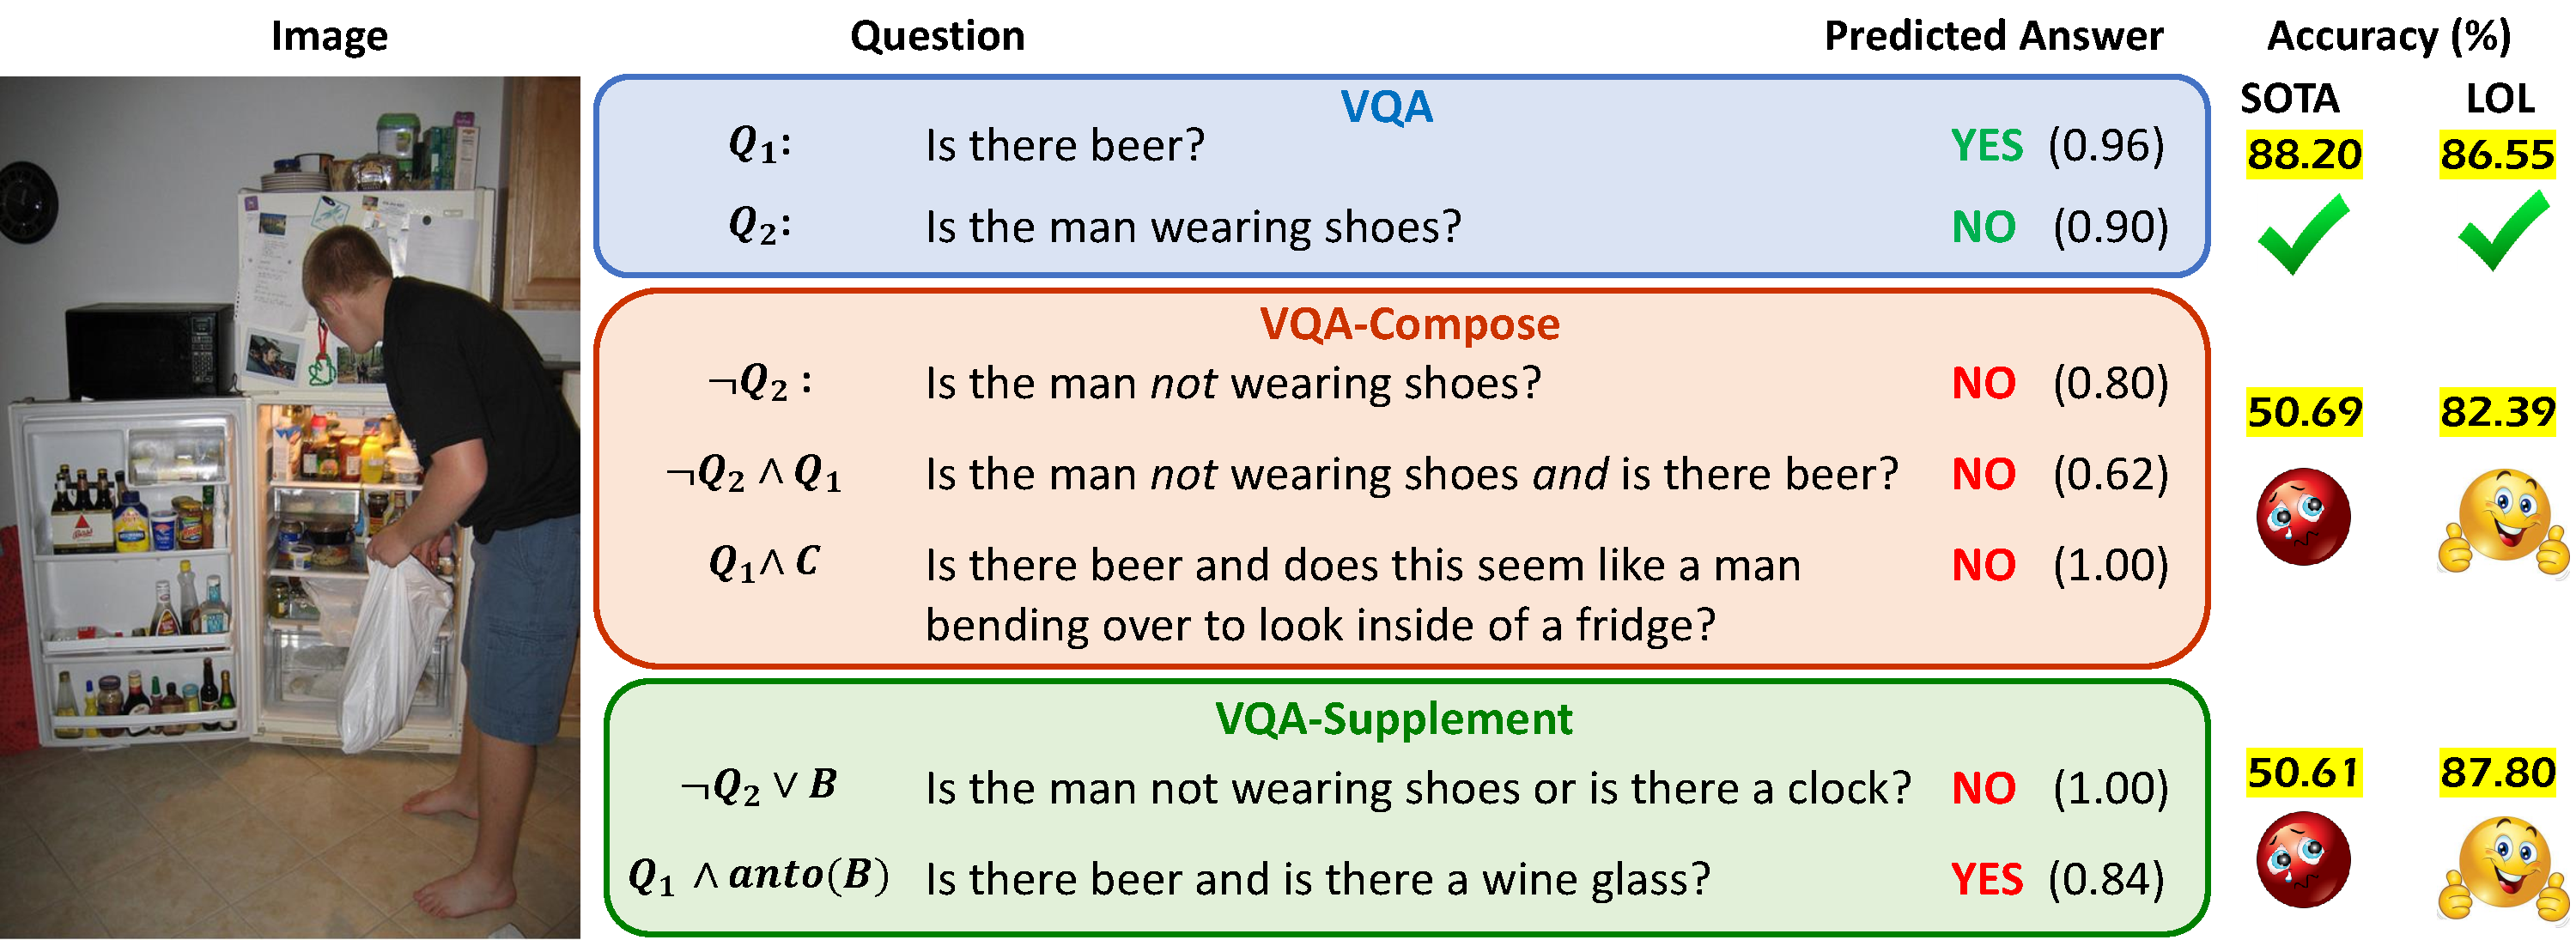
\includegraphics[width=\linewidth]{vqalol/images/teaser_final.pdf}
    \caption{
        % Illustration of logical composition of questions. 
        State-of-the-art models answer questions from the VQA dataset ($Q_1, Q_2$) correctly, but struggle when asked a logical composition including negation, conjunction, disjunction, and antonyms. 
        We develop a model that improves on this metric substantially, while retaining VQA performance.
        }
    \label{fig:motivation}
\end{figure}%
%%%%%%%%%%%%%%%%%%%%%%%%%%%%%%%%%%%%%%%%%%%%%%%%%%%%%%%%%%%%%%%%
\section{Introduction}
%%%%%%%%%%%%%%%%%%%%%%%%%%%%%%%%%%%%%%%%%%%%%%%%%%%%%%%%%%%%%%%%
Theories about logic in human understanding have a long history. 
In modern times, Piaget and Fodor~\citep{piattelli1980language} studied the representation of logical hypotheses in the human mind.
George Boole~\citep{boole1854investigation} formalized conjunction, disjunction, and negation into an ``algebra of thought'' as a way to improve, systemize, and mathematize Aristotle's Logic~\citep{corcoran1972completeness}.
Horn regarded negation to be a fundamental and defining characteristic of human communication~\citep{horn2000negation}, following the traditions of Sankara~\citep{raju1954principle}, Spinoza~\citep{spinoza1934ethics}, and Hegel~\citep{hegel1929hegel}.
Recent studies~\citep{arlotti1263} have suggested that infants can formulate intuitive and stable logical structures to interpret dynamic scenes and to entertain and rationally modify hypotheses about the scenes.
As such we argue that understanding logical structures in questions, is a fundamental requirement for any question-answering system.
\begin{quotation}
    \begin{quote}
        \textit{If a question can be put at all, then it can be answered.}\\\hspace*{\fill}{\citet{wittgenstein2013tractatus}}
    \end{quote}
\end{quotation}
In the above proposition, Wittgenstein linked the process of asking a question with the existence of an answer.
While we do not comment on the existence of an answer, we suggest the following softer proposition -
\begin{quotation}
    \begin{quote}
        \textit{If questions $Q_1\dots Q_n$ can be answered, then so should all composite questions created from $Q_1\dots Q_n$}
    \end{quote}
\end{quotation}

Visual question answering (VQA)~\citep{antol2015vqa} is an intuitive, yet challenging task that lies at a crucial intersection of vision and language. 
Given an image and a question about it, the goal of a VQA system is to provide a free-form or open-ended answer.
Consider the image in Figure~\ref{fig:motivation} which shows a person in front of an open fridge.
When asked the questions $Q_1$ ({\it Is there beer?}) and $Q_2$ ({\it Is the man wearing shoes?}) independently, the state-of-the-art model LXMERT~\citep{tan2019lxmert} answers both correctly.
However when we insert a negation in $Q_2$ ({\it Is the man not wearing shoes?}) or for a conjunction of two questions $\neg Q_2 \wedge Q1$ ({\it Is the man not wearing shoes and is there beer?}), the system makes wrong predictions. 
Our motivation is to reliably answer such logically composed questions.
In this paper, we analyze VQA systems under this {\it Lens of Logic (LOL)} and develop a model that can answer such questions reflecting human logical inference.
We offer our work as the first investigation into the logical structure of questions in visual question-answering and provide a solution that {\it learns} to interpret logical connectives in questions.

The first question is: can models pre-trained on the VQA dataset answer logically composed questions?
It turns out that these models are unable to do so, as illustrated in Figure~\ref{fig:motivation} and Table~\ref{table:exp1}.
An obvious next experiment is to \textit{split the question} into its component questions, predict the answer to each, and combine the answers logically. 
However language parsers (either oracle or trained parsers) are not accurate at understanding negation, and as such this approach does not yield correct answers for logically composed questions.
The question then arises: can the model answer such questions, if we explicitly train it with data that also contains logically composed questions?
For this investigation, we construct two datasets, \texttt{VQA-Compose} and \texttt{VQA-Supplement}, by utilizing annotations from the VQA dataset, as well as object and caption annotations from COCO~\citep{lin2014microsoft}.
We use these datasets to train the state-of-the-art model LXMERT~\citep{tan2019lxmert} and perform multiple experiments to test for robustness towards logically composed questions.

After this investigation, we develop our LOL model architecture that jointly learns to answer questions while understanding the type of question and which logical connective exists in the question, through our attention modules, as shown in Figure~\ref{fig:model}.
We further train our model with a novel Fréchet-Compatibility loss that ensures compatibility between the answers to the component questions and the answer of the logically composed question.
One key finding is that our models are better than existing models trained on logical questions, with a small deviation from state-of-the-art on VQA test set.
Our models also exhibit better {\it Compositional Generalization} i.e. models trained to answer questions with a single logical connective are able to answer those with multiple connectives.

Our contributions are summarized below:
\begin{enumerate}[noitemsep]
    \item We conduct a detailed analysis of the performance of the state-of-the-art VQA model with respect to logically composed questions,
    \item We curate two large scale datasets \texttt{VQA-Compose} and \texttt{VQA-Supplement} that contain logically composed binary questions.
    \item We propose \textit{LOL} -- our end-to-end model with dedicated attention modules that answer questions by understanding the logical connectives in questions.
    \item We show a capability of answering logically composed questions, while retaining VQA performance. % on VQA data.
\end{enumerate}

%%%%%%%%%%%%%%%%%%%%%%%%%%%%%%%%%%%%%%%%%%%%%%%%%%%%%%%%%%%%%%%%
\section{Related Work}
%%%%%%%%%%%%%%%%%%%%%%%%%%%%%%%%%%%%%%%%%%%%%%%%%%%%%%%%%%%%%%%%
\noindent\textbf{Logic in Human Expression:}
Is logical thinking a natural feature of human thought and expression?
Evidence in psychological studies~\citep{carey1985conceptual,gopnik1999scientist,arlotti1263} suggests that infants are capable of logical reasoning, toddlers understand logical operations in natural language and are able to compositionally compute meanings even in complex sentences containing multiple logical operators.
Children are also able to use these meanings to assign truth values to complex experimental tasks.
Given this, question-answering systems also need to answer compositional questions, and be robust to the manifestation of logical operators in natural language.\\

\noindent\textbf{Logic in Natural Language Understanding:}
The task of understanding compositionality in question-answering (QA) can also be interpreted as understanding logical connectives in text.
While question compositionality is largely unstudied, approaches in natural language understanding seek to transform sentences into symbolic formats such as first-order logic (FOL) or relational tables~\citep{mintz2009distant,zettlemoyer2012learning,lewis-steedman-2013-combined}.
While such methods benefit from interpretability, they suffer from practical limitations like intractability, reliance on background knowledge, and failure to process noise and uncertainty. 
\citep{bordes2013translating,riedel-etal-2013-relation,socher2013reasoning} suggest that better generalization can be achieved by learning embeddings to reason about semantic relations, and to simulate FOL behavior~\citep{rocktaschel2014low}.
Recursive neural networks have been shown to learn logical semantics on synthetic English-like sentences by using embeddings~\citep{bowman2014recursive,neelakantan2015compositional}.

Detection of negation in text has been studied for information extraction and sentiment analysis~\citep{morante2012modality}.
\citep{kassner2019negated} have shown that BERT-based models~\citep{devlin2018bert,liu2019roberta} are incapable of differentiating between sentences and their negations.
Concurrent to our work,~\citep{asai-hajishirzi-2020-logic} show the efficacy of FOL-guided data augmentation for performance improvements on natural language QA tasks that require reasoning.
Since our work deals with both vision and language modalities, it encounters a greater degree of ambiguity, thus calling for robust VQA systems that can deal with logical transformations.\\

\noindent\textbf{Visual Question Answering}
(VQA)~\citep{antol2015vqa} is a large-scale, human-annotated dataset for open-ended question-answering on images.
VQA-v2\citep{goyal2017making} reduces the language bias in the dataset by collecting complementary images for each question-image pair.
This ensures that the number of questions in the VQA dataset with the answer ``YES" is equal to those with the answer ``NO".
This dataset contains 204k images from MS-COCO~\citep{lin2014microsoft}, and 1.1M questions.

Cross-modal pre-trained models ~\citep{tan2019lxmert,lu2019vilbert,zhou2020unified} have proved to be highly effective in vision-and-language tasks such as VQA, referring expression comprehension, and image retrieval. 
While neuro-symbolic approaches~\citep{Mao2019NeuroSymbolic} have been proposed for VQA tasks which require reasoning on synthetic images, their performance on natural images is lacking.
Recent work seeks to incorporate reasoning in VQA, such as visual commonsense reasoning~\citep{zellers2019recognition,fang2020video2commonsense}, spatial reasoning~\citep{hudson2019gqa,johnson2017clevr}, and by integrating knowledge for end-to-end reasoning~\citep{Aditya:2019:IKR:3367722.3367926}.

We take a step back and extensively analyze the pivotal task of VQA with respect to various aspects of generalization.
We consider a rigorous investigation of a task, dataset, and models to be equally important as proposing new challenges that are arguably harder.
In this paper we analyse existing state-of-the-art VQA models with respect to their robustness to logical transformations of questions.

%%%%%%%%%%%%%%%%%%%%%%%%%%%%%%%%%%%%%%%%%%%%%%%%%%%%%%%%%%%%%%%%
\section{The Lens of Logic}
%%%%%%%%%%%%%%%%%%%%%%%%%%%%%%%%%%%%%%%%%%%%%%%%%%%%%%%%%%%%%%%%
\begin{table}[!t]
    \centering
    \begin{tabular}{@{}lp{8.6cm}lc@{}}
    \toprule 
    \textbf{QF} & \textbf{Question} & \textbf{AF} & \textbf{Answer}\\
    \midrule
    $Q_1$                       & Is there beer?                                    & $A_1$     & Yes \\
    $Q_2$                       & Is the man wearing shoes?                         & $A_2$     & No \\
    ${\neg}Q_1$                  & Is there no beer?                                 & ${\neg}A_1$ & No\\
    ${\neg}Q_2$                  & Is the man not wearing shoes?                     & ${\neg}A_2$ & Yes\\
    $Q_1{\wedge}Q_2$            & Is there beer and is the man wearing shoes?       & $A_1{\wedge}A_2$ & No \\
    $Q_1{\vee}Q_2$              & Is there beer or is the man wearing shoes?        & $A_1{\vee}A_2$ & Yes \\
    $Q_1{\wedge}{\neg}Q_2$       & Is there beer and is the man not wearing shoes?   & $A_1{\wedge}{\neg}A_2$ & Yes \\
    $Q_1{\vee}{\neg}Q_2$         & Is there beer or is the man not wearing shoes?    & $A_1{\vee}{\neg}A_2$ & Yes \\
    ${\neg}Q_1{\wedge}Q_2$       & Is there no beer and is the man wearing shoes?    & ${\neg}A_1{\wedge}A_2$ & No \\
    ${\neg}Q_1{\vee}Q_2$         & Is there no beer or is the man wearing shoes?     & ${\neg}A_1{\vee}A_2$ & No \\
    ${\neg}Q_1{\wedge}{\neg}Q_2$  & Is there no beer and is the man not wearing shoes?& ${\neg}A_1{\wedge}{\neg}A_2 $ & No \\
    ${\neg}Q_1{\vee}{\neg}Q_2$    & Is there no beer or is the man not wearing shoes? & ${\neg}A_1{\vee}{\neg}A_2$ & Yes \\
    \bottomrule
    \end{tabular}
    \caption{Illustration of question composition in \texttt{VQA-Compose}, for the same example as in Figure \ref{fig:motivation}.
    QF: Question Formula, AF: Answer Formula}
    \label{tab:compose}
\end{table}

\begin{figure}[t]
    \centering
    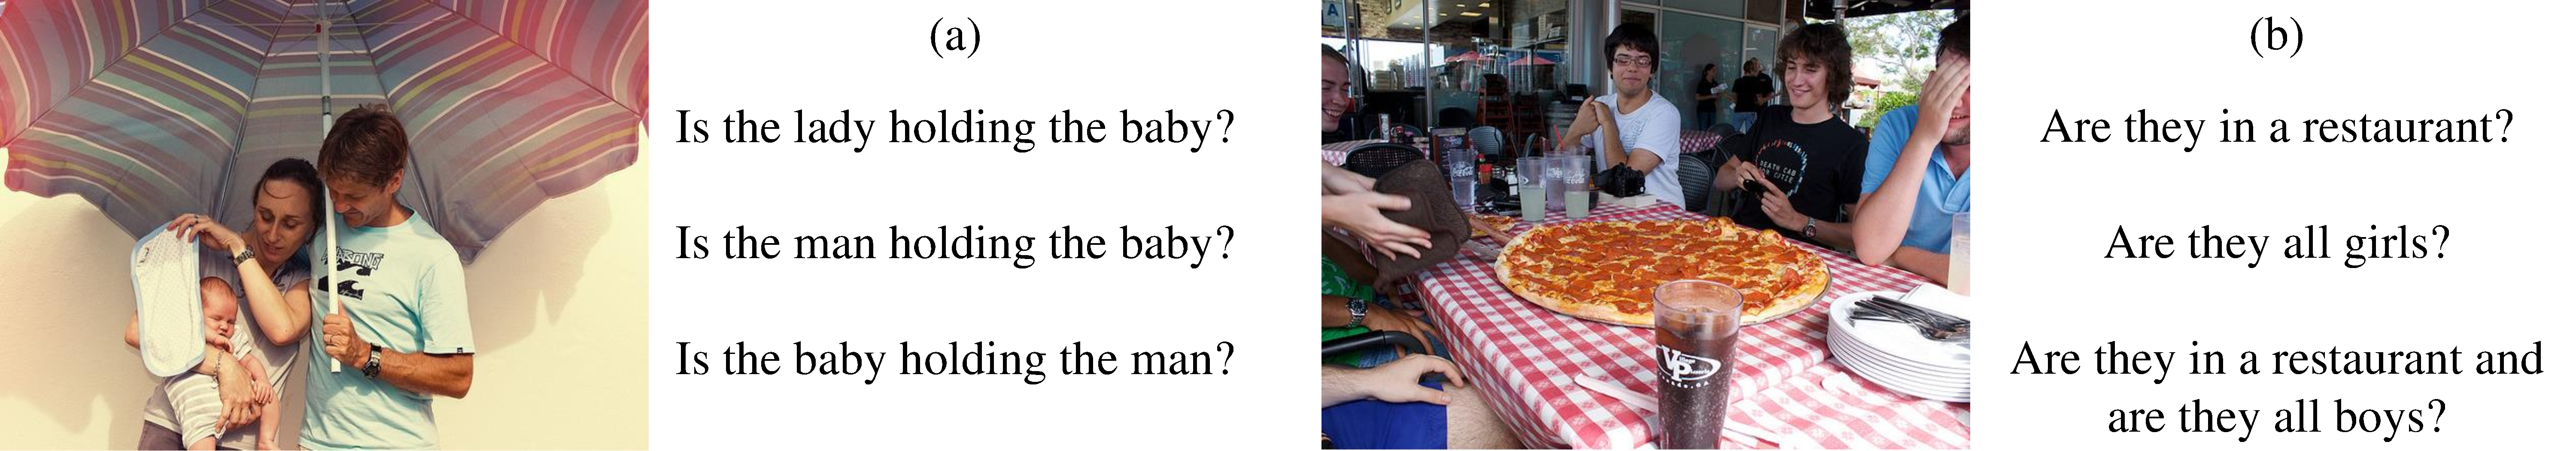
\includegraphics[width=\linewidth]{vqalol/images/illus.pdf}
    \caption{Some questions in \texttt{VQA-Supplement} created with adversarial antonyms.}
    \label{fig:illus}
\end{figure}

A lens magnifies objects under investigation, by allowing us to zoom and focus on desired contents or processes.
Our lens of logical composition of questions, allows us to magnify, identify, and analyze the problems in VQA models.

Consider Figure~\ref{fig:illus}(a), where we transform the first question {\it ``Is the lady holding the baby"} by first replacing {\it ``lady"} with an adversarial antonym {\it ``man"} and observe that the system provides a wrong answer with very high probability.
Swapping {\it ``man"} with {\it ``baby"} results in a wrong answer as well.
In~\ref{fig:illus}(b) a conjunction of two questions containing antonyms ({\it girls} vs {\it boys}) yields a wrong answer.
We identify that the ability to answer composite questions created by negation, conjunction and disjunction of questions is crucial for VQA.

We use ``closed questions" as defined in~\citep{bobrow1964natural} to construct logically composed questions. 
Under this definition, if a closed question has a negative (``NO") answer then its negation must have an affirmative (``YES") answer.
Of the three types of questions in the VQA dataset (yes/no, numeric, other), `yes-no" questions satisfy this requirement.
Although, visual questions in the VQA dataset can have multiple correct answers~\citep{bhattacharya2019does}, $20.91\%$ of the questions (around 160k) in the VQA dataset are closed questions, i.e. questions with a single unambiguous yes-or-no answer, unanimously annotated by multiple human workers.
This allows us to treat these questions as propositions and create a truth table for answers to compose logical questions as shown in Table~\ref{tab:compose}.

    \subsection{Composite Questions}
    Let $\mathcal{D}$ be the VQA dataset. 
    For closed questions $Q_1$ and $Q_2$ about image $I\in\mathcal{D}$, we define the composite question $Q^*$ composed using connective $\circ\in\{ \vee, \wedge\}$, as:
    \begin{equation}
        Q^* = \widehat{Q_1} ~\circ ~\widehat{Q_2}, \qquad where~~ \widehat{Q_1} \in \{ Q_1, \neg Q_1\},  ~ \widehat{Q_2} \in \{ Q_2, \neg Q_2\}. 
    \end{equation}
    
    \subsection{Dataset Creation Process}
    Using the above definition we create two new datasets by utilizing multiple questions about the same image (\texttt{VQA-Compose}) and external object and caption annotations about the image from COCO to create more questions (\texttt{VQA-Supplement}).
    The seed questions for creating these datasets are all closed binary questions from VQA-v2~\citep{goyal2017making}.
    These datasets serve as test-beds, and enable experiments that analyze performance of models when answering such questions.\\

        \noindent\textbf{VQA-Compose:}
        Consider the first two rows in Table~\ref{tab:compose}. 
        $Q_1$ and $Q_2$ are two questions about the image in Figure~\ref{fig:motivation} taken from the VQA dataset.
        Additional questions are composed from $Q_1$ and $Q_2$ by using the formulas in Table~\ref{tab:compose}.
        Thus for each pair of closed questions in the VQA dataset, we get 10 logically composed questions.
        Using the same train-val-test split as the VQA-v2 dataset~\citep{goyal2017making}, we get \textit{1.25 million samples} for our \texttt{VQA-Compose} dataset.
        The dataset is balanced in terms of the number of questions with affirmative and negative answers.\\
        
        \noindent\textbf{VQA-Supplement:}
        Images in VQA-v2 follow identical train-val-test splits as their source MS-COCO~\citep{lin2014microsoft}.
        Therefore, we use the object annotations from COCO to create additional closed binary questions, such as {\it ``Is there a bottle"} for the example in Figure~\ref{fig:motivation}.
        We also create ``adversarial" questions about objects, like {\it ``Is there a wine-glass?"} by using an object that is not present in the image (wine-glass), but is \textit{semantically close} to an object in the image (bottle).
        We use Glove vectors~\citep{pennington2014glove} to find the adversarial object with the closest embedding. 
        Following a similar strategy, we also convert captions provided in COCO to closed binary questions, for example {\it ``Does this seem like a man bending over to look inside the fridge"}.
        Since we know what objects are present in the image, and the captions describe a ``true" scene, we are able to obtain the ground-truth answers for questions created from objects and captions.
        Similar methods for creation of question-answer pairs have previously been used in~\citep{ren2015exploring,malinowski2014multi}.

        Thus for every question, we obtain several questions from objects and captions, and use these to compose additional questions by following a process similar to the one for \texttt{VQA-Compose}.
        For each closed question in the VQA dataset, we get $20$ additional logically composed questions by utilizing questions created from objects and captions, yielding a total of \textit{2.55 million samples} as \texttt{VQA-Supplement}.

    \subsection{Analytical Setup}
    In order to test the robustness of our models to logically composed questions, we devise five key experiments to analyse baseline models and our methods.
    These experiments help us gain insights into the nuances of the VQA dataset, and allow us to develop strategies for promoting robustness.\\

        \noindent\textbf{Effect of Data Augmentation:}
        In this experiment, we compare the performance of models on \texttt{VQA-Compose} and \texttt{VQA-Supplement} with or without logically composed training data.
        This experiment allows us to test our hypotheses about the robustness of any VQA model to logically composed questions.
        We first use models trained on VQA data to answer questions in our new datasets and record performance.
        We then explicitly train the same models with our new datasets, and make a comparison of performance with the pre-trained baseline.\\
        
        \noindent\textbf{Learning Curve:}
        We train our models with an increasing number of logically composed questions and compare performance.
        This serves as an analysis of the number of logical samples needed by the model to understand logic in questions.\\
    
        \noindent\textbf{Training only with Closed Questions:}
        In this ablation study, we restrict the training data to only closed questions i.e. ``Yes-No" VQA questions, \texttt{VQA-Compose} and \texttt{VQA-Supplement}, allowing our model to focus solely on closed questions.\\
    
        \noindent\textbf{Compositional Generalization:}
        We address whether training on closed questions containing single logical operation ($\neg Q_1$,  $Q_1\vee Q_2$) can generalize to multiple operations ($Q_1 \wedge \neg Q_2$, $\neg Q_1 \vee Q_2$).
        For instance, rows 1 through 6 in Table~\ref{tab:compose} are {\it single operation questions}, while rows 7 through 12 are {\it multi-operation questions}.
        Our aim is to have models that exhibit such compositional generalization.\\
        
        \noindent\textbf{Inductive Generalization:}
        We investigate if training on compositions of two questions ($\neg Q_1 \vee Q_2$) can generalize to compositions of more than two questions ($Q_1 \wedge \neg Q_2 \wedge Q_3 \dots$).
        This studies whether our models develop an understanding of logical connectives, as opposed to simply learning patterns from large data.

%%%%%%%%%%%%%%%%%%%%%%%%%%%%%%%%%%%%%%%%%%%%%%%%%%%%%%%%%%%%%%%%
\section{Method}
%%%%%%%%%%%%%%%%%%%%%%%%%%%%%%%%%%%%%%%%%%%%%%%%%%%%%%%%%%%%%%%%
\begin{figure}[t]
    \centering
    \includegraphics[width=\linewidth]{vqalol/images/vqa_lol_eccv.png}
    \caption{LOL model architecture showing a cross-modal feature encoder followed by our Question-Attention ($q_{\textit{\tiny ATT}}$) and Logic Attention ($\ell_{\textit{\tiny ATT}}$) modules. 
    The concatenated output of  is used by the Answering Module to predict the answer.
    % to the question (Q).
    }
    \label{fig:model}
\end{figure}

In this section. we describe LXMERT~\citep{tan2019lxmert} (a state-of-the-art VQA model), our Lens of Logic (LOL) model, attention modules which learn the question-type and logical connectives in the question, and the Fréchet-Compatibility (FC) Loss.
This section refers to a composition of two questions, but applies to $n\geq2$ questions.

    \subsection{Cross-Modal Feature Encoder}
    LXMERT (Learning Cross-Modality Encoder Representations from Transformers)~\citep{tan2019lxmert} is one of the first cross-modal pre-trained frameworks for vision-and-language tasks, that combines a strong visual feature extractor~\citep{ren2015faster} with a strong language model (BERT)\citep{devlin2018bert}.
    LXMERT is pre-trained for key vision-and-language tasks, on a large corpus of $\sim$9M image-sentence pairs, making it a powerful cross-modal encoder for vision+language tasks such as visual question answering, as compared to other models such as MCAN~\citep{Yu_2019_CVPR} and UpDn~\citep{Anderson2017up-down}, and strong representative baseline for our experiments.


    \subsection{Our Model: Lens of Logic (LOL)}
    The design for our LOL model is driven by three key insights:
    \begin{enumerate}[noitemsep]
        \item As logically composed questions are closed questions, understanding the type of question will guide the model to answer them correctly.
        \item Predicted answers must be compatible with the predicted question type. For instance, a closed question can have an answer that is either ``Yes" or ``No".
        \item The model must learn to identify the logical connectives in a question.
    \end{enumerate}

    \noindent Given these insights, we develop the Question Attention module that encodes the type of question (\textit{Yes-No}, \textit{Number}, or \textit{Other}), and the Logic Attention module that predicts the connectives (\textit{AND, OR, NOT, no connective}) present in the question, and use these to learn representations.
    The overall model architecture is shown in Figure~\ref{fig:model}.
    For every question $Q$ and corresponding image $I$, we obtain embeddings $z_Q$ and $z_I$ respectively, as well as a cross-modal embedding $z_X$. 

        \textbf{Question Attention Module ($q_{\textit{ATT}}$)}
        takes cross-modal embedding $z_x$ from LXMERT as input, and outputs vector \textbf{$P_{type} = softmax(\mathbf{q_{\textit{\tiny ATT}}}(z_x))$}, representing the probabilities of each question-type. 
        These probabilities are used to get a final representation $\mathbf{z^{type}}$ which combines the features for each question-type.\footnotemark[1]

        \textbf{Logic Attention Module ($\ell_{\textit{ATT}}$)}
        takes the cross-modal embedding $z_X$ from LXMERT as input, and outputs vector \textbf{$P^{conn} = \sigma(\mathbf{\ell_{\textit{ATT}}}(z_X))$} which represents the probabilities of each type of connective.
        We use sigmoid ($\sigma$) instead of a softmax, since a question can have multiple connectives.
        These probabilities are used to combine the features for each type of connective into a final representation $\mathbf{z^{conn}}$ which encodes information about the connectives in the question.

    \subsection{Loss Functions}
    We train our models jointly with the loss function given by:
    \begin{equation}
        \mathcal{L} = (1{-}\alpha_1{-}\alpha_2)\cdot \mathcal{L}_{ans} + \alpha_1 \cdot \mathcal{L}_{type} + \alpha_2 \cdot \mathcal{L}_{conn} + \beta\cdot\mathcal{L}_{\mathit{FC}}.
    \end{equation}

        \noindent\textbf{Answering Loss} $\ell_{ans}$ is conditioned on the type of question.
        We multiply the final prediction vector with the probability and the mask $M_i$ for question-type $i$.
        $M_i$ is a binary vector with $1$ for every answer-index of type-i and $0$ elsewhere:
        
        \begin{equation}
            \mathcal{L}_{\textit{ans}} = \mathcal{L}_{\textit{\tiny BCE}}(\sum_{i=1}^{3}\hat{y} \odot M_i \cdot P^{\textit{type}}_i, y_{\textit{ans}}).
        \end{equation}
        
        \noindent\textbf{Attention Losses:}
        $q_{\textit{\tiny ATT}}$ is trained to minimize a Negative Log Likelihood (NLL) classification loss, ensuring a shrinkage of probabilities of the answer choices of the wrong type. $\ell_{\textit{\tiny ATT}}$ is trained to minimize a multi-label classification loss, using Binary Cross-Entropy (BCE) given by:
        \begin{align}
            \mathcal{L}_{\textit{type}} &= \mathcal{L}_{\textit{\tiny NLL}}(\text{softmax}(z^{\textit{type}}), y_{\textit{type}}),\\
             \mathcal{L}_{\textit{conn}} &= \mathcal{L}_{\textit{\tiny BCE}}(\sigma(z^{\textit{conn}}), y_{\textit{conn}}),
        \end{align}
        where $y_{ans}, y_{type}, y_{conn}$ are labels for answer, question-type and connective.\\

        \noindent\textbf{Fréchet-Compatibility Loss:}
        We introduce a new loss function that ensures compatibility between the answers predicted by the model for the component questions $Q_1$ and $Q_2$ and the composed question $Q$.
        Let $A, A_1, A_2$ be the respective answers predicted by the model for $Q$, $Q_1$, and $Q_2$. $Q_i$ can have negation.
        Then Fréchet inequalities~\citep{boole1854investigation,frechet1935generalisation} provide us with bounds for the probabilities of the answers of the conjunction and disjunction of the two questions:
        \begin{align}
            \mathit{max}(0, p(A_1)+p(A_2)-1) &\leq p(A_1 \wedge A_2) \leq \mathit{min}(p(A_1), p(A_2)). \\
            \mathit{max}(p(A_1), p(A_2)) &\leq p(A_1 \vee A_2) \leq \mathit{min}(1, p(A_1) + p(A_2)).
        \end{align}
        We define ``Fréchet bounds" $b_L$ and $b_R$ to be the left and right bounds for the triplet $A, A_1, A_2$,
        and the ``Fréchet Mean" $m_A$ to be the average of the Fréchet bounds; $m_A = (b_L + b_R)/2$.
        Then, the Fréchet-Compatibility Loss given by:
        \begin{equation}
            \mathcal{L}_{FC} = (p(A) - \mathbbm{1}(m_A > 0.5))^2, 
        \end{equation}
        ensures that the predicted answer and that determined by $m_A$ match. 

    \subsection{Implementation Details}
    The LXMERT feature encoder produces a vector $z$ of length 768 which is used by our attention modules, each having sub-networks $\mathbf{f_i}, \mathbf{g_i}$ with 2 feed-forward layers.
    We first train our models without FC loss.
    Then we select the best models with a checkpoint of 10 epochs and finetune these further for 3 epochs with FC loss, since the FC loss is designed to work for a model whose predictions are not random.
    Thus our improvements in accuracy are attributable to the FC Loss and not more training epochs.
    We utilize the Adam optimizer~\citep{kingma2014adam} with a learning rate of $5\textit{e-}5$, batch size of 32 and train for 20 epochs.
    Our models are trained on 4 NVIDIA V100 GPUs, and take approximately 24 hours for training 20 epochs.\footnote{More training details in Supplementary Materials}
    

%%%%%%%%%%%%%%%%%%%%%%%%%%%%%%%%%%%%%%%%%%%%%%%%%%%%%%%%%%%%%%%%%%%%%%%%%%%%%%%%
\section{Experiments}
%%%%%%%%%%%%%%%%%%%%%%%%%%%%%%%%%%%%%%%%%%%%%%%%%%%%%%%%%%%%%%%%%%%%%%%%%%%%%%%%
\begin{table}
    \centering
    % \resizebox{0.85\linewidth}{!}{
    \begin{tabular}{p{0.15\linewidth} p{0.3\linewidth} cccc}
    \toprule
    & & \multicolumn{4}{c}{\textbf{Validation Accuracy (\%) $\uparrow$}}\\
    \cmidrule{3-6}
    \textbf{Model} & \textbf{Trained on} & VQA & YN & Comp & Supp \\
    \toprule
    \multirow{3}{*}{\footnotesize LXMERT}
    & VQA &               68.94 & \textbf{86.65} & 50.79 & 50.51 \\
    & VQA + Comp &        67.85 & 85.32 & 85.03 & 80.85 \\
    & VQA + Comp + Supp & 68.83 & 84.83 & 70.28 & 85.17 \\

    \textit{ \footnotesize with FC Loss} & VQA + Comp + Supp & 67.84 &	84.92 & 75.31 &	85.25 \\
    \midrule
    \multirow{3}{*}{{\footnotesize LOL (qATT)}}
    & VQA &               \underline{\textbf{69.08}} & \underline{85.32} & 48.99 & 50.54 \\
    & VQA + Comp &        67.51 & 84.82 & 84.85 & 79.62 \\
    & VQA + Comp + Supp & 68.72 & 84.99 & 79.88 & 87.12 \\
    \midrule
    
    \multirow{3}{*}{\pbox{25mm}{\footnotesize LOL (Full)}}
    & VQA + Comp &        68.94 & 85.15 & \underline{\textbf{85.13}} & 79.02\\
    & VQA + Comp + Supp & 68.86 & 84.87 & 81.07 & 87.54\\

    \textit{ \footnotesize with FC Loss} & VQA + Comp + Supp & 68.10 &	84.75 & 82.39 &	\underline{\textbf{87.80} }\\
    
    \midrule 
    \midrule
    %% YES-NO only training
    \multirow{2}{*}{{\footnotesize LXMERT}}
    & YN + Comp & - & 84.13 & 84.44 & 79.39 \\
    & YN + Comp + Supp & - & 84.09 & 82.63 & 88.15 \\ 
    \midrule 
    
    %% YES-NO only training
    \multirow{2}{*}{{\footnotesize LOL ($\ell$ATT})}
    & YN + Comp & - & 85.22 & \underline{\textbf{85.31}} & 79.87 \\
    & YN + Comp + Supp & - & 85.26 & 84.37 & \underline{\textbf{89.00}}\\ 
    \bottomrule
    \end{tabular}
    % }
    \caption[Comparison of LXMERT and LOL when trained on VQA dataset and the combinations of VQA and \texttt{VQA-Compose}, \texttt{VQA-Supplement}.]{Comparison of LXMERT and LOL trained on VQA data, combinations with \texttt{Compose}, \texttt{Supplement}, and our Frechet-Compatibility (FC) Loss \footnotemark}
    
    \label{table:exp1}
\end{table}
\footnotetext{In all tables, best overall scores are bold, our best scores underlined.}
We first conduct analytical experiments to test for logical robustness and transfer learning capability.
We use three datasets for our experiment: the VQA v2.0~\citep{antol2015vqa} dataset, a combination of VQA and our \texttt{VQA-Compose} dataset, and a combination of VQA, \texttt{VQA-Compose} and \texttt{VQA-Supplement}.
The size of the training dataset and the distribution of yes-no, number and other questions is kept the same as the original VQA dataset ($\sim$443k) for fair comparison.
Since \texttt{VQA-Supplement} uses captions and objects from MS-COCO, we use is to analyze the ability of our models to generalize to a new source of data (MS-COCO) as well as questions containing adversarial objects.
After training, our attention modules ($q_{\textit{ATT}}$ and $\ell_{\textit{ATT}}$) achieve an accuracy of 99.9\% on average, showing almost perfect performance when it comes to learning the type of question and the logical connectives present in the question.

\begin{table}
    \centering
    \begin{tabular}{p{2cm} c c cc c cc}
        \toprule
        \multirow{2}{*}{\textbf{Model}} &  & \hphantom & \multicolumn{2}{c}{\textbf{VQA-Compose}} & \hphantom &  \multicolumn{2}{c}{\textbf{VQA-Supplement}}\\
        \cmidrule{4-5} \cmidrule{7-8}
         & \textbf{YN} & & Single & Multiple & & Single & Multiple\\
        \toprule
        \multirow{1}{*}{\pbox{10mm}{\footnotesize LXMERT}}
        % & YN + C          & 84.16 & 84.71  & 65.60 & 80.63 & 66.55 \\
        & 85.07 & & 83.95 & 61.99 & & 86.65 & 60.00 \\
        \midrule
        \multirow{1}{*}{\footnotesize LOL}
        % & YN + C & \underline{\textbf{85.13}} & \underline{\textbf{85.85}} & \underline{\textbf{66.87}} & 81.66 & \underline{\textbf{79.10}}\\
        & 85.12 & & 84.60 & 66.03 & & \underline{\textbf{87.42}} & 66.05  \\
        \bottomrule
        % \multirow{2}{*}{\pbox{15mm}{\footnotesize LXMERT + \\Type + Conn}}
        % & YN + C & 85.17 & 81.88 & \textbf{70.58} & 90.76 & 46.19 \\
        % & YN + C + S & 85.19 & 81.16 & 57.76 & 91.88 & 47.76  \\
        % \hline
    \end{tabular}
    \begin{tabular}{p{2cm} cc c cc}
        \toprule
        \multirow{2}{*}{\textbf{Model}} & \multicolumn{2}{c}{\textbf{VQA-Compose}} & \hphantom &  \multicolumn{2}{c}{\textbf{VQA-Supplement}}\\
        \cmidrule{2-3} \cmidrule{5-6}
        & $Q_1\circ~Q_2$ & $Q_2\circ~Q_1$ & & $Q_1\circ~Q_2$ & $Q_2\circ~Q_1$\\
        \toprule
        \multirow{1}{*}{\pbox{10mm}{\footnotesize LXMERT}} & 
        82.34 & 80.44 & & 85.57 & 81.78\\
        \midrule
        \multirow{1}{*}{\footnotesize LOL} & 84.91 & 83.64 & & 85.62 & 83.41\\
        \bottomrule
        % \multirow{2}{*}{\pbox{15mm}{\footnotesize LXMERT + \\Type + Conn}}
        % & YN + C & 85.17 & 81.88 & \textbf{70.58} & 90.76 & 46.19 \\
        % & YN + C + S & 85.19 & 81.16 & 57.76 & 91.88 & 47.76  \\
        % \hline
    \end{tabular}
    \caption[Generalization]{Validation accuracies ($\%$) for Compositional Generalization and Commutative Property. Note that 50\% is random performance.\footnotemark[2]}
    \label{table:exp4}
\end{table}
\begin{figure}[t]
    \centering
    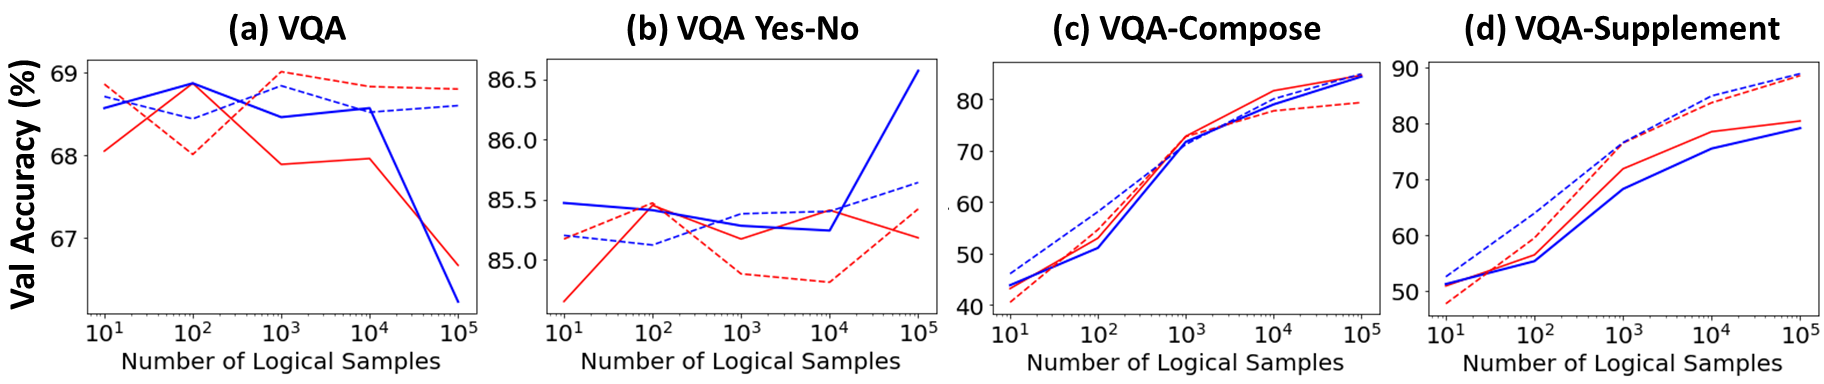
\includegraphics[width=\linewidth]{vqalol/images/fig_exp3_new.png}
    \caption{
    % Learning Curves: Red lines denote LXMERT, Blue lines denote our LOL model with $q_{\textit{ATT}}$. 
    % Models trained on VQA + \texttt{Comp} are shown in solid and those trained on VQA + \texttt{Comp} + \texttt{Supp} are in dotted lines. Best viewed in color.
    Learning Curve comparison for models (Red: LXMERT, Blue: LOL) trained on our datasets (solid lines: VQA~+~\texttt{Comp}, dotted lines: VQA~+~\texttt{Comp}~+~\texttt{Supp})
    }
    \label{fig:exp3}
\end{figure}


    \subsection{Can't We Just Parse the Question into Components?}
    
    Since our questions are a composition of multiple questions, an obvious approach is to split the question into its components, and to discern the logical formula for composition.
    The answers to these component questions (predicted by VQA models) can be \textit{re-combined} with the predicted logical formula to obtain the final answer.
    We use parsers to map components and logical operations to predefined slots in a logical function.
    The oracle parser uses the ground truth component questions and combines predicted answers using the true formula.
    However, at test time we do not have access to the true mapping and components.
    So we train a RoBERTa-Base~\citep{liu2019roberta} parser using B-I-O tagging~\citep{ramshaw-marcus-1995-text} for a Named-Entity Recognition task with constituent questions as entities.\footnotemark[1]
    
    The performance of the oracle parser serves as the upper bound as we have a perfect mapping, with the QA system being the only source of error.
    The trained parser has an exact-match accuracy of $85\%$, but only a $72\%$ accuracy in determining the number of operands.
    The parser has an accuracy of $89\%$ for questions with 3 or less operands, but only $78\%$ for longer compositions.
    End-to-end (E2E) models do not need to parse questions and hence overcome these hurdles, but do require an understanding of logical operations.
    Table~\ref{table:sota} shows that both oracle and trained parsers when used with LOL outperform parsers with LXMERT, by $6.82\%$) and $5.60\%$ respectively.
    The LOL model without using any parsers is better than both LXMERT and LOL with the trained parser by $7.55\%$ and $1.95\%$ respectively.

    \subsection{Explicit Training with Logically Composed Questions}
    \noindent\textbf{Can models trained on the VQA-v2 dataset answer logically composed questions?}
    The first section of Table~\ref{table:exp1} shows that LXMERT, when trained only on questions from VQA-v2 has near random accuracy ($\sim$50\%) on our logically composed datasets, thus exhibiting little robustness to such questions.\\
    
    \noindent\textbf{Can baseline model improve if trained explicitly with logically composed questions questions?}
    We train the models with data containing a combination of samples from VQA-v2, \texttt{VQA-Compose}, and \texttt{VQA-Supplement}.
    The accuracy on \texttt{VQA-Compose} and \texttt{VQA-Supplement} 
    improves, but there is a drop in performance on yes-no questions from VQA.
    Our models with our attention modules ($q_{\textit{\tiny ATT}}$ and $\ell_{\textit{\tiny ATT}}$) are able to retain performance on VQA-v2 while achieving improvements on all validation datasets.


    \subsection{Analysis}

        \noindent\textbf{Training with Closed Questions only:}
        We analyse the performance of models when trained only with closed questions from VQA, VQA + \texttt{Comp} and VQA + \texttt{Comp} + \texttt{Supp} and see that our model achieves the best accuracy on logically composed questions, as shown in sections 3 and 4 in Table~\ref{table:exp1}.
        Since we train only closed questions, we do not use our question attention module for this experiment.\\
        
        \noindent\textbf{Effect of Logically Composed Questions:}
        We increase the number of logical samples in the training data on a log scale from 10 to 100k.
        As can be seen from the learning curves in Figure~\ref{fig:exp3}(a), models trained on VQA + \texttt{Comp} + \texttt{Supp} are able to retain performance on VQA validation data, while those trained only on VQA + \texttt{Comp} data deteriorate.
        Figure~\ref{fig:exp3}(b) shows that our models improve on VQA Yes-No performance after being trained on more logically composed samples, exhibiting transfer learning capabilities.
        In (c) both our models are comparable to the baseline, but our model shows improvements over the baseline when trained on VQA + \texttt{Comp} + \texttt{Supp}.
        In (d) for all levels of additional logical questions, our model trained on VQA + \texttt{Comp} + \texttt{Supp} is the best performing.
        From (c) and (d), we observe that a large number of logical questions are needed during training for the models to learn to answer them during inference.
        We also see that our model yields the best performance on \texttt{VQA-Supplement}.\\
        
        \noindent\textbf{Compositional Generalization:}
        To test for compositional generalization, we train models on questions with a maximum of one connective (single) and test on those with multiple connectives.
        It can be seen from Table~\ref{table:exp4} that our models are better equipped than the baseline to generalize to multiple connectives and also to be able to generalize from \texttt{VQA-Compose} to \texttt{Supplement}.\\
        
            \begin{figure}
        \centering
            \subfloat[\label{heatmap_comp}]{%
            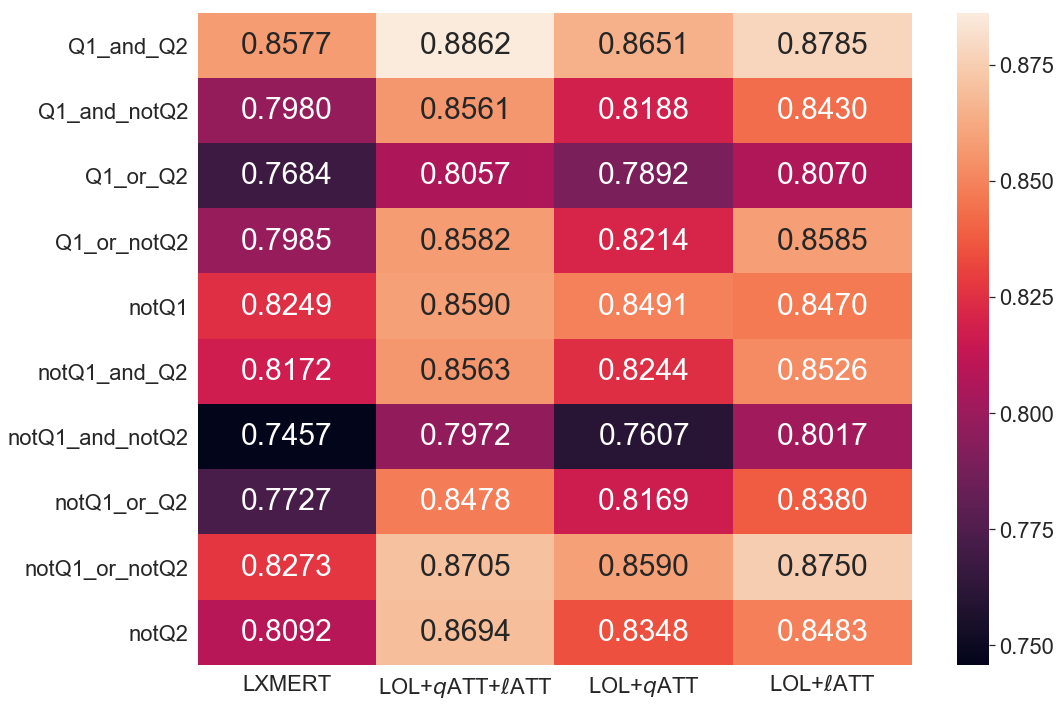
\includegraphics[angle=0,origin=c,width=0.6\linewidth]{vqalol/images/lol_heatmap.png}
            }\\
            \subfloat[\label{heatmap_supp}]{%
            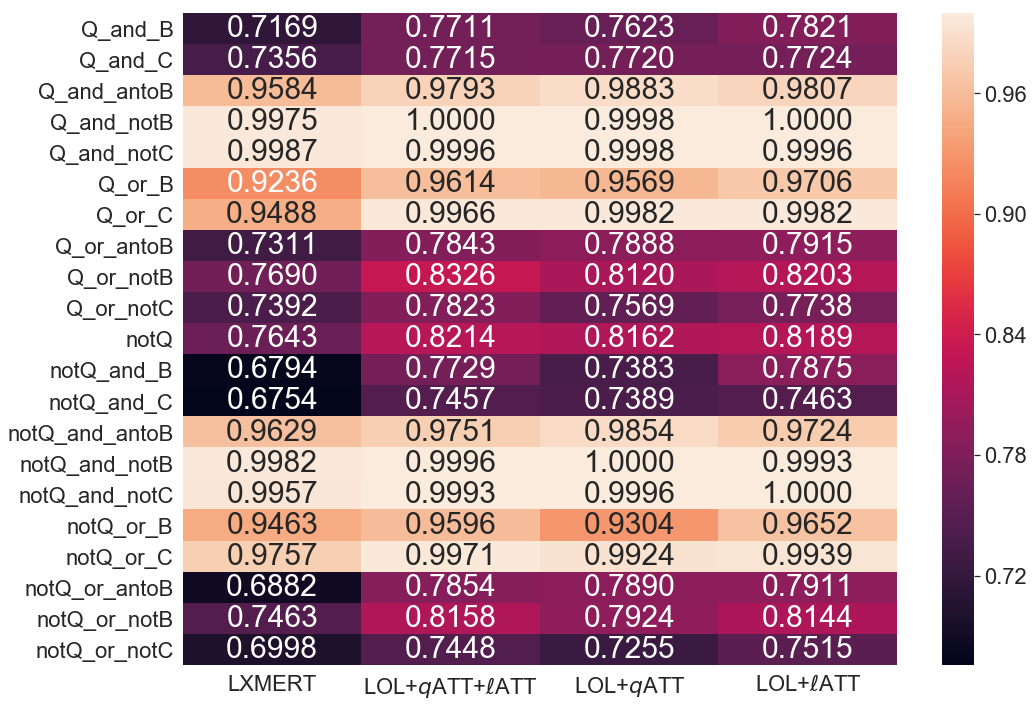
\includegraphics[angle=0,origin=c,width=0.65\linewidth]{vqalol/images/cwl_heatmap.png}
            }\\
            \subfloat[\label{varlen}]{%
            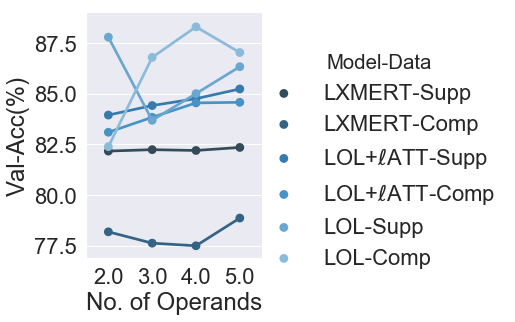
\includegraphics[angle=0,origin=c,width=0.4\linewidth]{vqalol/images/varlen_fixed2.png}
            }
        \caption{Accuracy for each type of question in (a) VQA-Compose, (b) VQA-Supplement and for questions with number of operands greater than 2.}
        \label{fig:heatmap}
    \end{figure}
        
        \noindent\textbf{Inductive Generalization:}
        We test our models on questions composed with more than two components. Parser-based  models have this property by default.
        As shown by Figure~\ref{varlen} our E2E models outperform the baseline LXMERT.\\

        \noindent\textbf{Commutative Property:}
        Our models have identical answers when the question is composed either as $Q_1\circ Q_2$ or $Q_2\circ Q_1$, for logical operation $\circ$, as shown in Table~\ref{table:exp4}.
        The parser-based models are agnostic to the order of components if the parsing is accurate, while our E2E models are robust to the order.\\

        \noindent\textbf{Accuracy per Category of Question Composition:}
        In Figure~\ref{fig:heatmap} we show a plot of accuracy versus question type for each model.
        $Q, Q_1, Q_2$ are questions from VQA, $B, C$ are object-based and caption-based questions from COCO respectively.
        From the results, we interpret that questions such as $Q\wedge antonym(B), Q\wedge\neg B, Q\wedge\neg C$ are easy because the model is able to understand absence of objects, therefore can always answer these questions with a ``NO".
        Similarly, $ Q\vee B, Q\vee C$ are easily answered since presence of the object makes the answer always ``YES".
        By simply understanding object presence many such questions can be answered. Figure~\ref{fig:heatmap} shows the model has the same accuracy for logically equivalent operations.

    \begin{table*}[t]
    \centering
     \resizebox{\linewidth}{!}{
    \begin{tabular}{@{}lllcccccccc@{}}
    \toprule
    \multirow{2}{*}{Model} & \multirow{2}{*}{Parser} & \multirow{2}{*}{\textbf{\pbox{20mm}{Training \\Data}}} & \multicolumn{4}{c}{\textbf{Test-Std. Accuracy (\%) $\uparrow$}} & \hphantom & \multicolumn{3}{c}{\textbf{Val. Accuracy (\%) $\uparrow$}}\\
     \cmidrule{4-7} \cmidrule{9-11}
     & & & Yes-No & Number & Other & Overall & & {Compose} & Supplement & Overall \\
    \midrule
    MCAN & None & VQA~\citep{Yu_2019_CVPR} & $86.82^{\#}$ & $53.26^{\#}$ & $60.72^{\#}$ & 70.90 & & 52.42 & {*} & {*}\\
    LXMERT & None & VQA~\citep{tan2019lxmert} & \textbf{88.20} & \textbf{54.20} & \textbf{63.10} & \textbf{72.50} & & 50.79 & 50.51 & 50.65\\
    LOL ($\mathit{q}$ATT) & None & VQA &  \underline{87.33} & \underline{54.03} & \underline{62.40} & \underline{72.03} & & 48.99 & 50.54 & 49.77\\
    \midrule
    LXMERT & Oracle & VQA & 88.20 & 54.20 & 63.10 & 72.50 & & 86.38 & 74.29 & 80.33 \\
    LXMERT & Trained & VQA & 88.20 & 54.20 & 63.10 & 72.50 & & 86.35 & 68.75 & 77.55\\
    LOL (full) & Oracle & VQA+Ours & 86.55 & 53.42 & 61.58 &71.04 & & 85.79 & 88.51 & 87.15\\
    LOL (full) & Trained & VQA+Ours & 86.55 & 53.42 & 61.58 &71.04 & & 82.13 & 84.17 & 83.15\\
    \midrule
    LXMERT & None & VQA+Ours & 85.23 & 51.25 & 60.58 & 69.78 & & 75.31 & 85.25 & 80.28 \\
    % LOL & None & VQA+Ours & 86.55 & 53.42 & 61.58 & 71.04 & & 72.88 & 88.32 \\
    LOL ($\mathit{q}$ATT) & None & VQA+Ours &  86.79 & 52.66 & 61.85 & 71.19 & & 79.88 & 87.12 & 83.50\\
    LOL (full)
    % ($\mathit{q}$ATT+$\ell$ATT) 
    & None & VQA+Ours & 86.55 & 53.42 & 61.58 &71.04 & & \underline{\textbf{82.39}} & \underline{\textbf{87.80}} & 85.10\\
    \bottomrule
    \end{tabular}
    }
    \caption[Test Set Results]{Performance on `test-standard' set of VQA-v2 and validation set of our datasets. LOL performance is close to SOTA on VQA-v2, but significantly better at logical robustness. $^*$\text{MCAN} uses a fixed vocabulary 
    % so we are unable to evaluate on 
    that prohibits evaluation on \texttt{VQA-Supplement} which has questions created from COCO captions. 
    $^{\#}$Test-dev scores, since MCAN does not report test-std single-model scores\footnotemark[2]}
    \label{table:sota}
\end{table*}
    \subsection{Evaluation on VQA v2.0 Test Data}
    Table~\ref{table:sota} shows the performance the VQA Test-Standard datset.
    Our models maintain overall performance on the VQA test dataset, and at the same time substantially improve from random performance ($\sim$ 50\%) on logically composed questions to 82.39\% on \texttt{VQA-Compose} and 87.80\% on \texttt{VQA-Supplement}.
    This shows that logical connectives in questions can be learned while not degrading the overall performance on the original VQA test set (our models are within $\sim$1.5\% of the state-of-the-art on all three types of questions on the VQA test-set).
    

%%%%%%%%%%%%%%%%%%%%%%%%%%%%%%%%%%%%%%%%%%%%%%%%%%%%%%%%%%%%%%%%%%%%%%%%%%%%%%%%
\section{Discussion}
%%%%%%%%%%%%%%%%%%%%%%%%%%%%%%%%%%%%%%%%%%%%%%%%%%%%%%%%%%%%%%%%%%%%%%%%%%%%%%%%
Consider the example, {\it ``Is every boy who is holding an apple or a banana, not wearing a hat?"}, humans are able to answer it to be true if and only if each boy who is holding \textit{at least one} of an apple or a banana is not wearing a hat~\citep{arlotti1263}.
Natural language contains such complex logical compositions, not to mention ambiguities and the influence of context.
In this paper, we focus on the simplest -- negation, conjunction, and disjunction.
We have shown that existing VQA models are not robust to questions composed with these logical connectives, even when we train parsers to split the question into its components.
When humans are faced with such questions, they may refrain from giving binary (Yes/No) answers.
For instance, logically, the question{\it ``Did you eat the pizza and did you like it?"} has a negative answer if either of the two component questions has a negative answer.
However, humans might answer the same question with the answer {\it ``Yes, but I did not like it"}.
While human question-answering is indeed elaborate, explanatory, and clarifying, that is the scope of our future work; here we focus only on predicting a single binary answer.

We have shown how connectives in a question can be identified by enhancing LXMERT encoders with dedicated attention modules and loss functions.
We would like to stress on the fact that we do not use knowledge of the connectives during inference, but instead train the network to be aware of it based on cross-modal features, instead of predicting purely based on language model embeddings which fail to capture these nuances.
% This work is an attempt to modularize the understanding of logical components to train the model to utilize the outputs of the attention modules.
We believe this work has potential implications on logic-guided data augmentation, logically robust question answering, and for conversational agents (with or without images).
Similar strategies and learning mechanisms will be used in the next chapter to operate ``logically'' in the image-space at the level of object classes and their attributes.


% \section{Conclusion}
% In this work, we investigate VQA in terms of logical robustness.
% The key hypothesis is that the ability to answer questions about an image, must be extendable to a logical composition of two such questions.
% We show that state-of-the-art models trained on VQA dataset lack this.
% Our solution involves the ``Lens of Logic" model architecture that learns to answer questions with negation, conjunction, and disjunction.
% We provide \texttt{VQA-Compose} and \texttt{VQA-Supplement}, two datasets containing logically composed questions to serve as benchmarks.
% Our models show improvements in terms of answering these questions, while at the same time retaining performance on the original VQA test-set.

% \section*{Acknowledgments}
% Support from NSF Robust Intelligence Program (1816039 and 1750082), DARPA (W911NF2020006) and ONR (N00014-20-1-2332) is gratefully acknowledged.
\chapter{Data Mutation for Robustness to Changing Priors}
\label{chap:mutant}
While progress has been made on the visual question answering leaderboards, models often utilize spurious correlations and priors in datasets under the i.i.d. setting. 
As such, evaluation on out-of-distribution (OOD) test samples has emerged as a proxy for generalization.
In this paper, we present \textit{MUTANT}, a training paradigm that exposes the model to perceptually similar, yet semantically distinct \textit{mutations} of the input, to improve OOD generalization, such as the VQA-CP challenge.
Under this paradigm, models utilize a consistency-constrained training objective to understand the effect of semantic changes in input (question-image pair) on the output (answer).
Unlike existing methods on VQA-CP, \textit{MUTANT} does not rely on the knowledge about the nature of train and test answer distributions.
\textit{MUTANT} establishes a new state-of-the-art accuracy on VQA-CP with a $10.57\%$ improvement.
Our work opens up avenues for the use of semantic input mutations for OOD generalization in question answering.
% \end{abstract}

%%%%%%%%%%%%%%%%%%%%%%%%%%%%%%%%%%%%%%%%%%%%%%%%%%%%%%%%%%%%%%%%
% INTRODUCTION
%%%%%%%%%%%%%%%%%%%%%%%%%%%%%%%%%%%%%%%%%%%%%%%%%%%%%%%%%%%%%%%%
\section{Introduction}
\begin{figure}
    \centering
    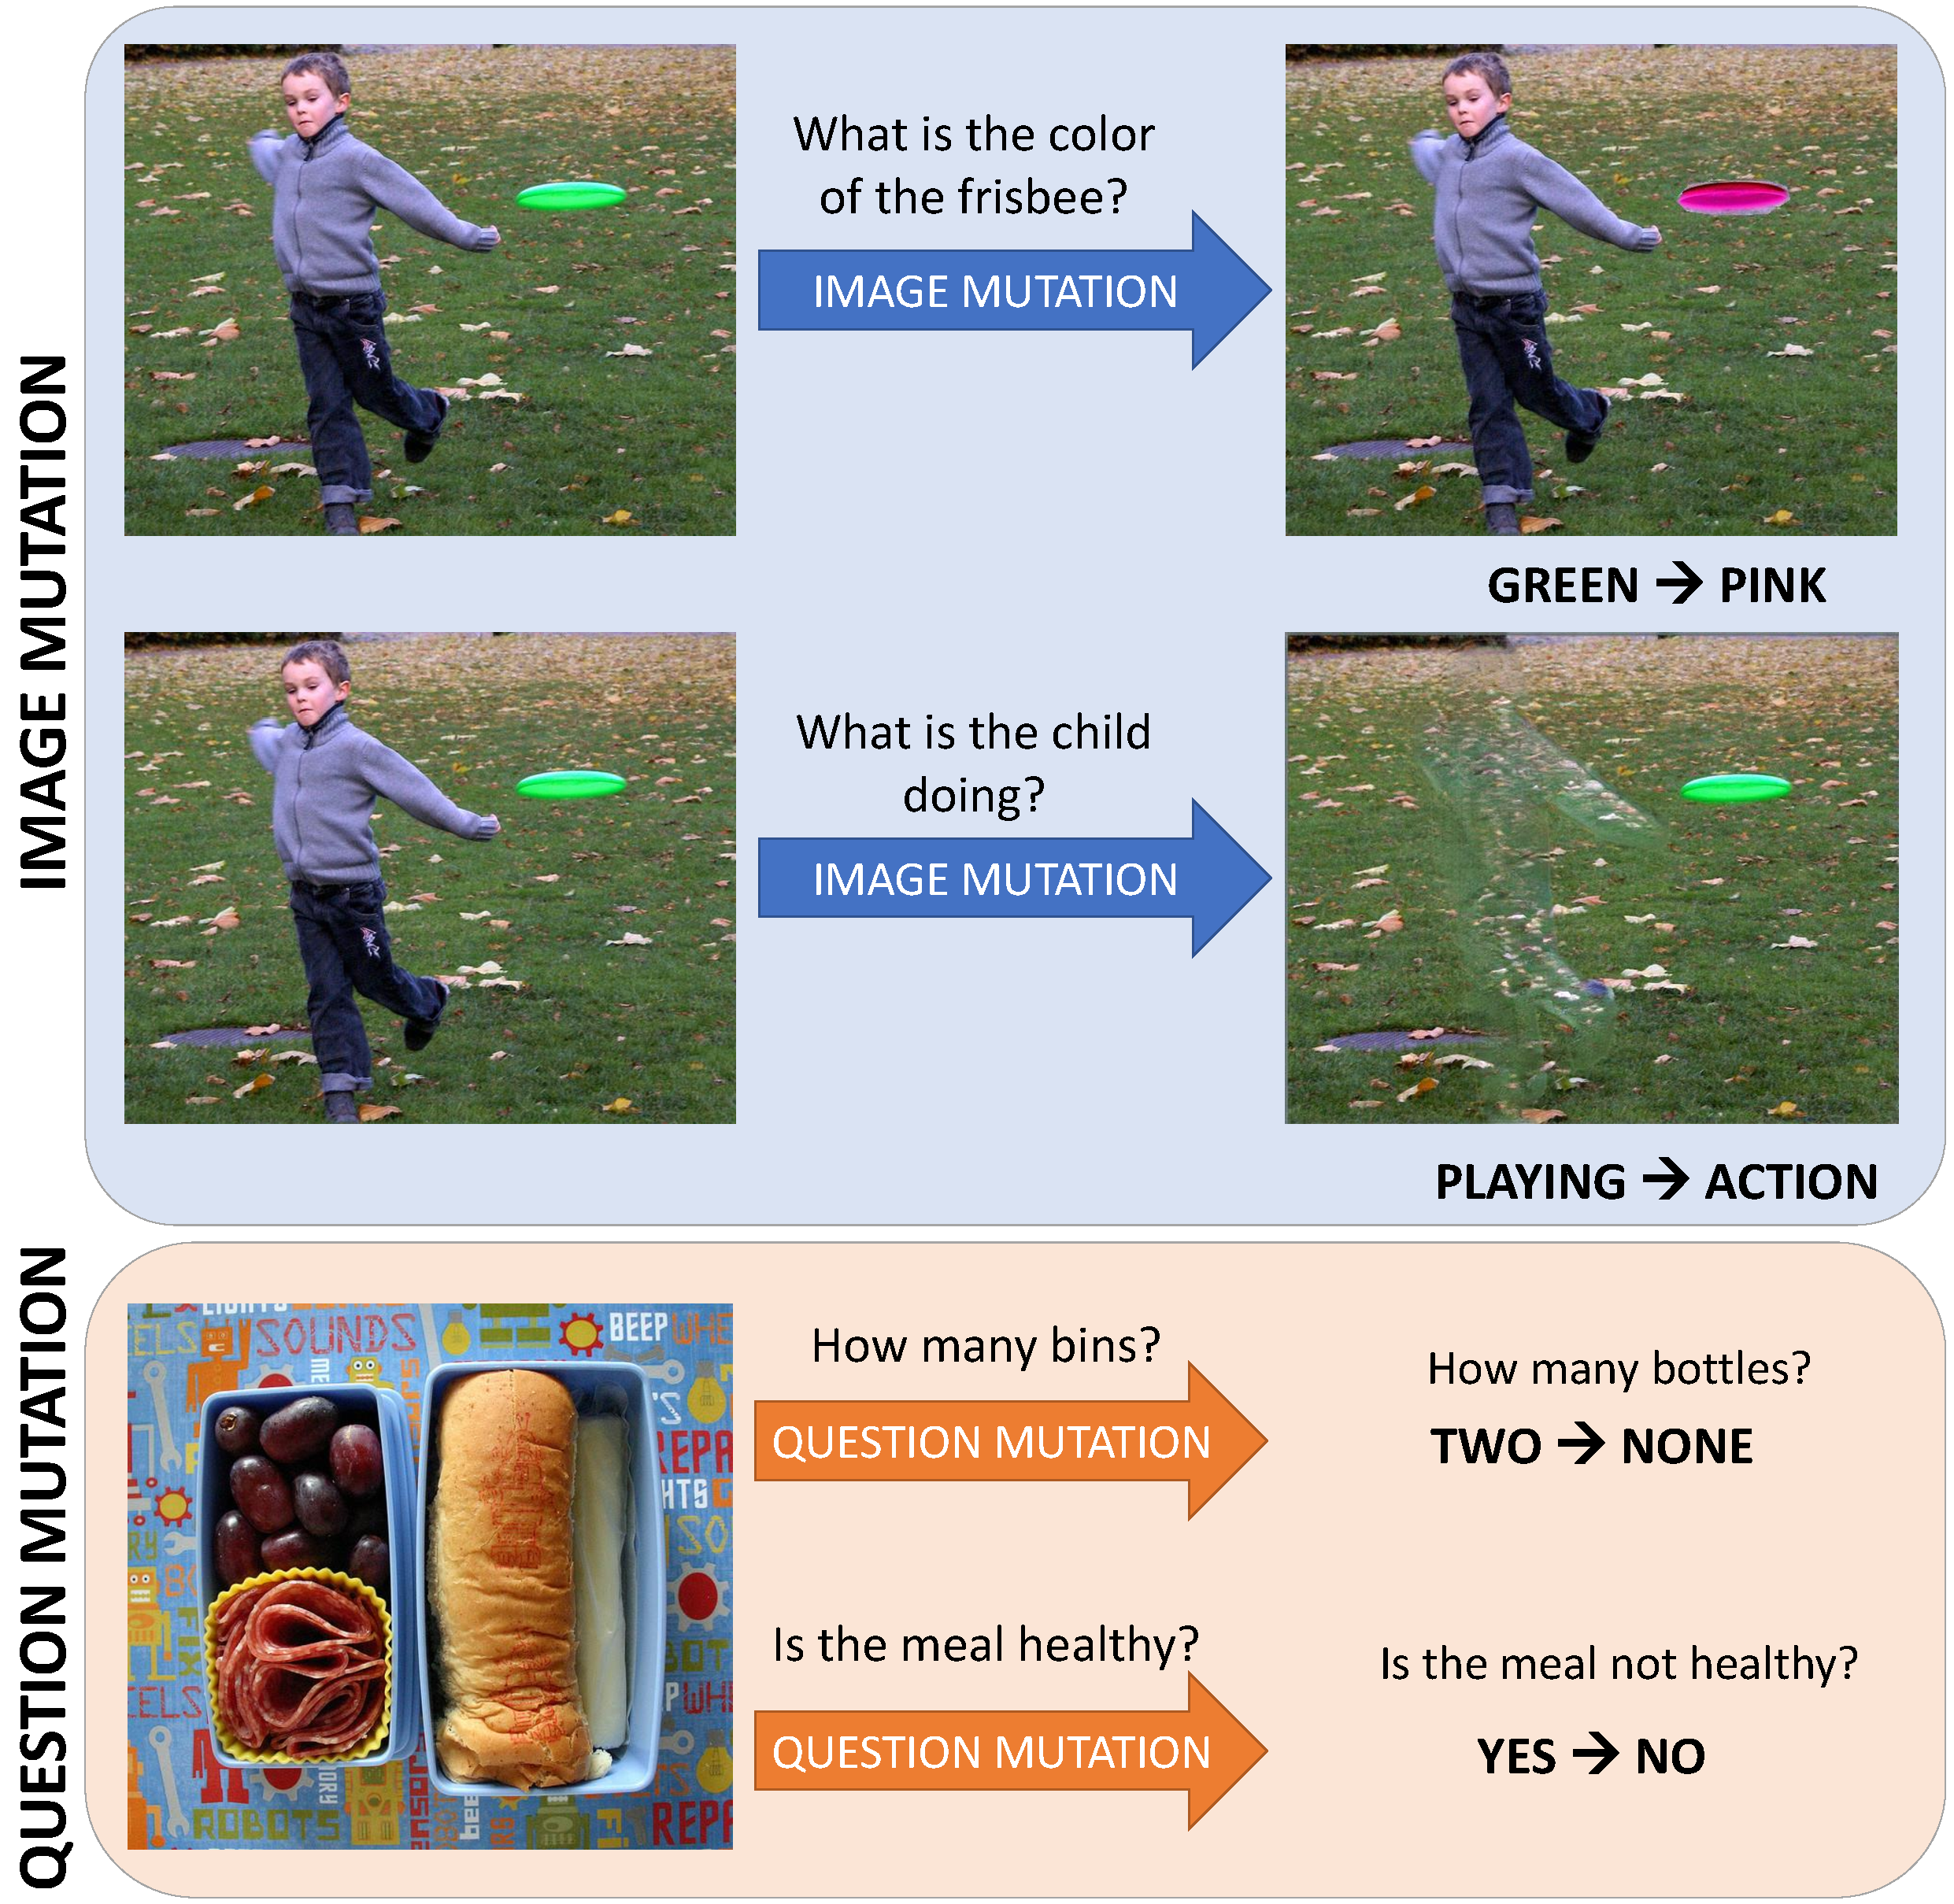
\includegraphics[width=0.8\linewidth]{mutant/figures/teaser.pdf}
    \caption{Illustration of the mutant samples. The input mutation, either by manipulating the image or the question, results in a change in the answer.}
    \label{fig:teaser}
\end{figure}


Availability of large-scale datasets has enabled the use of statistical machine learning in vision and language understanding, and has lead to significant advances.
However, the commonly used evaluation criterion is the performance of models on test-samples drawn from the same distribution as the training dataset, which cannot be a measure of generalization.
Training under this ``independent and identically distributed" (i.i.d.)~setting can drive decision making to be highly influenced by dataset biases and spurious correlations as shown in both natural language inference~\citep{kaushik2018much,poliak2018hypothesis,mccoy2019right} and visual question answering~\citep{goyal2017making,vqa-cp,selvaraju2020squinting}.
As such, evaluation on out-of-distribution (OOD) samples has emerged as a metric for generalization.

Visual question answering (VQA)~\citep{antol2015vqa} is a task at the crucial intersection of vision and language.
The aim of VQA models is to provide an answer, given an input image and a question about it.
Large datasets~\citep{antol2015vqa} have been extensively used for developing VQA models.
However over-reliance on datasets can cause models to learn spurious correlations such as linguistic priors~\citep{vqa-cp} that are specific to certain datasets and do not generalize to ``Out-of-Distribution" (OOD) samples, as shown in Figure~\ref{fig:teaser}.
While learning patterns in the data is important, learning dataset-specific spurious correlations is not a feature of robust VQA models.
Developing robust models has thus become a key pursuit for recent work in visual question answering through data augmentation~\citep{goyal2017making}, reorganization~\citep{vqa-cp}.

Every dataset contains biases; indeed inductive bias is \textit{necessary} for machine learning algorithms to work.
\citet{mitchell1980need} states that an unbiased learner's ability to classify is no better than a look-up from memory.
However this bias has a component which is useful for generalization (positive bias), and a component due to spurious correlations (negative bias).
We use the term ``positive bias" to denote the correlations that are necessary to perform a task --- for instance, the answer to a ``What sport is \dots" question is correlated to a name of a sport.
The term ``negative bias" is used for spurious correlations tat may be learned from the data --- for instance, always predicting ``tennis" as the answer to ``What sport\dots" questions.
The goal of OOD generalization is to mitigate negative bias while learning to perform the task.
However existing methods such as LMH~\citep{clark2019don}
try to remove all biases between question-answer pairs, by penalizing examples that can be answered without looking at the image;
we believe this to be counter-productive.
The analogy of antibiotics which are designed to remove pathogen bacteria, but also end up removing useful gut microbiome~\citep{willing2011shifting} is useful to understand this phenomenon.

We present a method that focuses on increasing positive bias and mitigating negative bias, to address the problem of OOD generalization in visual question answering.
Our approach is to enable the \textbf{mutation} of inputs (questions and images) in order to expose the VQA model to perceptually similar yet semantically dissimilar samples. 
The intuition 
is to implicitly allow the model to understand the critical changes in the input which lead to a change in the answer.
This concept of mutations is illustrated in Figure~\ref{fig:teaser}.
If the color of the frisbee is changed, or the child removed, i.e. \textit{when an image-mutation is performed}, the answer to the question changes.
Similarly, if a word is substituted by an adversarial word (bins$\rightarrow$bottles), an antonym, or negation (healthy$\rightarrow$not healthy), i.e. \textit{when a question-mutation is performed}, the answer also changes.
Notice that both mutations do not significantly change the input, most of the pixels in the image and words in the question are unchanged, and the type of reasoning required to answer the question is unchanged.
However the mutation significantly changes the answer.

In this work, we use this concept of mutations to enable models to focus on parts of the input that are critical to the answering process, by training our models to produce answers that are consistent with such mutations.
We present a question-type exposure framework which teaches the model that although such linguistic priors may exist in training data
(such as the dominant answer ``tennis" to ``What sport is ..." questions),
other sports can also be answers to such questions, thus mitigating negative bias.
This is in contrast to \citet{chen2020counterfactual} who focus on using data augmentation as a means for mitigating language bias.
This work takes a step away from explicit de-biasing as a method for OOD generalization and instead proposes amplification of positive bias and implicit attenuation of spurious correlations as the objective. Our contributions are as follow.
% \begin{itemize}[nosep,noitemsep]
%     \item We introduce the Mutant paradigm for training VQA models and the sample-generation mechanism which takes advantage of semantic transformations of the input image or question, for the goal of OOD generalization.
%     \item In addition to the conventional classification task, we formulate a novel training objective using Noise Contrastive Estimation over the projections of cross-modal features and answer embeddings on a shared projection manifold, to predict the correct answer.
%     \item Our pairwise consistency loss acts as a regularization that seeks to bring the distance between ground-truth answer vectors closer to the distance between predicted answer vectors for a pair of original and mutant inputs.
%     \item Extensive experiments and analyses demonstrate advantages of our method on the VQA-CP dataset, and establish a new state-of-the-art of $\mathbf{69.52\%}$, an improvement of $\mathbf{10.57\%}$.

% \end{itemize}


%%%%%%%%%%%%%%%%%%%%%%%%%%%%%%%%%%%%%%%%%%%%%%%%%%%%%%%%%%%%%%%%
% METHOD
%%%%%%%%%%%%%%%%%%%%%%%%%%%%%%%%%%%%%%%%%%%%%%%%%%%%%%%%%%%%%%%%
\section{MUTANT}
We consider the open-ended VQA problem as a multi-class classification problem.
The VQA dataset $\mathcal{D} = \{Q_i, I_i, a_i\}_{i=1}^N$ consists of questions $Q_i \in \mathcal{Q}$ and images $I_i \in {I}$, and answers $a_i \in \mathcal{A}$.
Many contemporary VQA models such as Up-Dn~\citep{anderson2018bottom} and LXMERT~\citep{tan2019lxmert} first extract cross-modal features from the image and question using attention layers, and then use these features as inputs to a neural network answering module which predicts the answer classes.
In this section we define our Mutant paradigm under this formulation of the VQA task.

    \subsection{Concept of Mutations}
    Let $X = (Q, I)$ denote an input to the VQA system with true answer $a$.
    A \textit{mutant} input $X^*$ is created by a small transformation in the image $(Q, I^*)$ or in the question $(Q^*, I)$ such that this transformation leads to a new answer $a^*$, as shown in Figure~\ref{fig:teaser}.
    There are three categories of transformation $T$ that create the mutant input $X^* = T(X)$, addition, removal, or substitution. 
    For image mutations, these correspond to addition or removal of objects, and morphing the attributes of the objects, such as color, texture, and lighting conditions. 
    For instance addition or removal of a person from the image in Figure~\ref{fig:image_mutation} changes the answer to the question ``How many persons are pictured".
    Question mutations can be performed by addition of a negative word (``no", ``not", etc.) to the question, masking critical words in the question, and substituting an object-word with an antonym or adversarial word.
    Thus for each sample in the VQA dataset, we can obtain a mutant sample and use it for training.

%%%%%%%%%%%%%%%%%%%%%%%%%%%%%%%%%%%%%%%%%%%%%%%%%%%%%%%%%%%%%%%%
% EXPERIMENTS
%%%%%%%%%%%%%%%%%%%%%%%%%%%%%%%%%%%%%%%%%%%%%%%%%%%%%%%%%%%%%%%%
\section{Generating Input Mutations for VQA}
\begin{figure}[t]
    \centering
    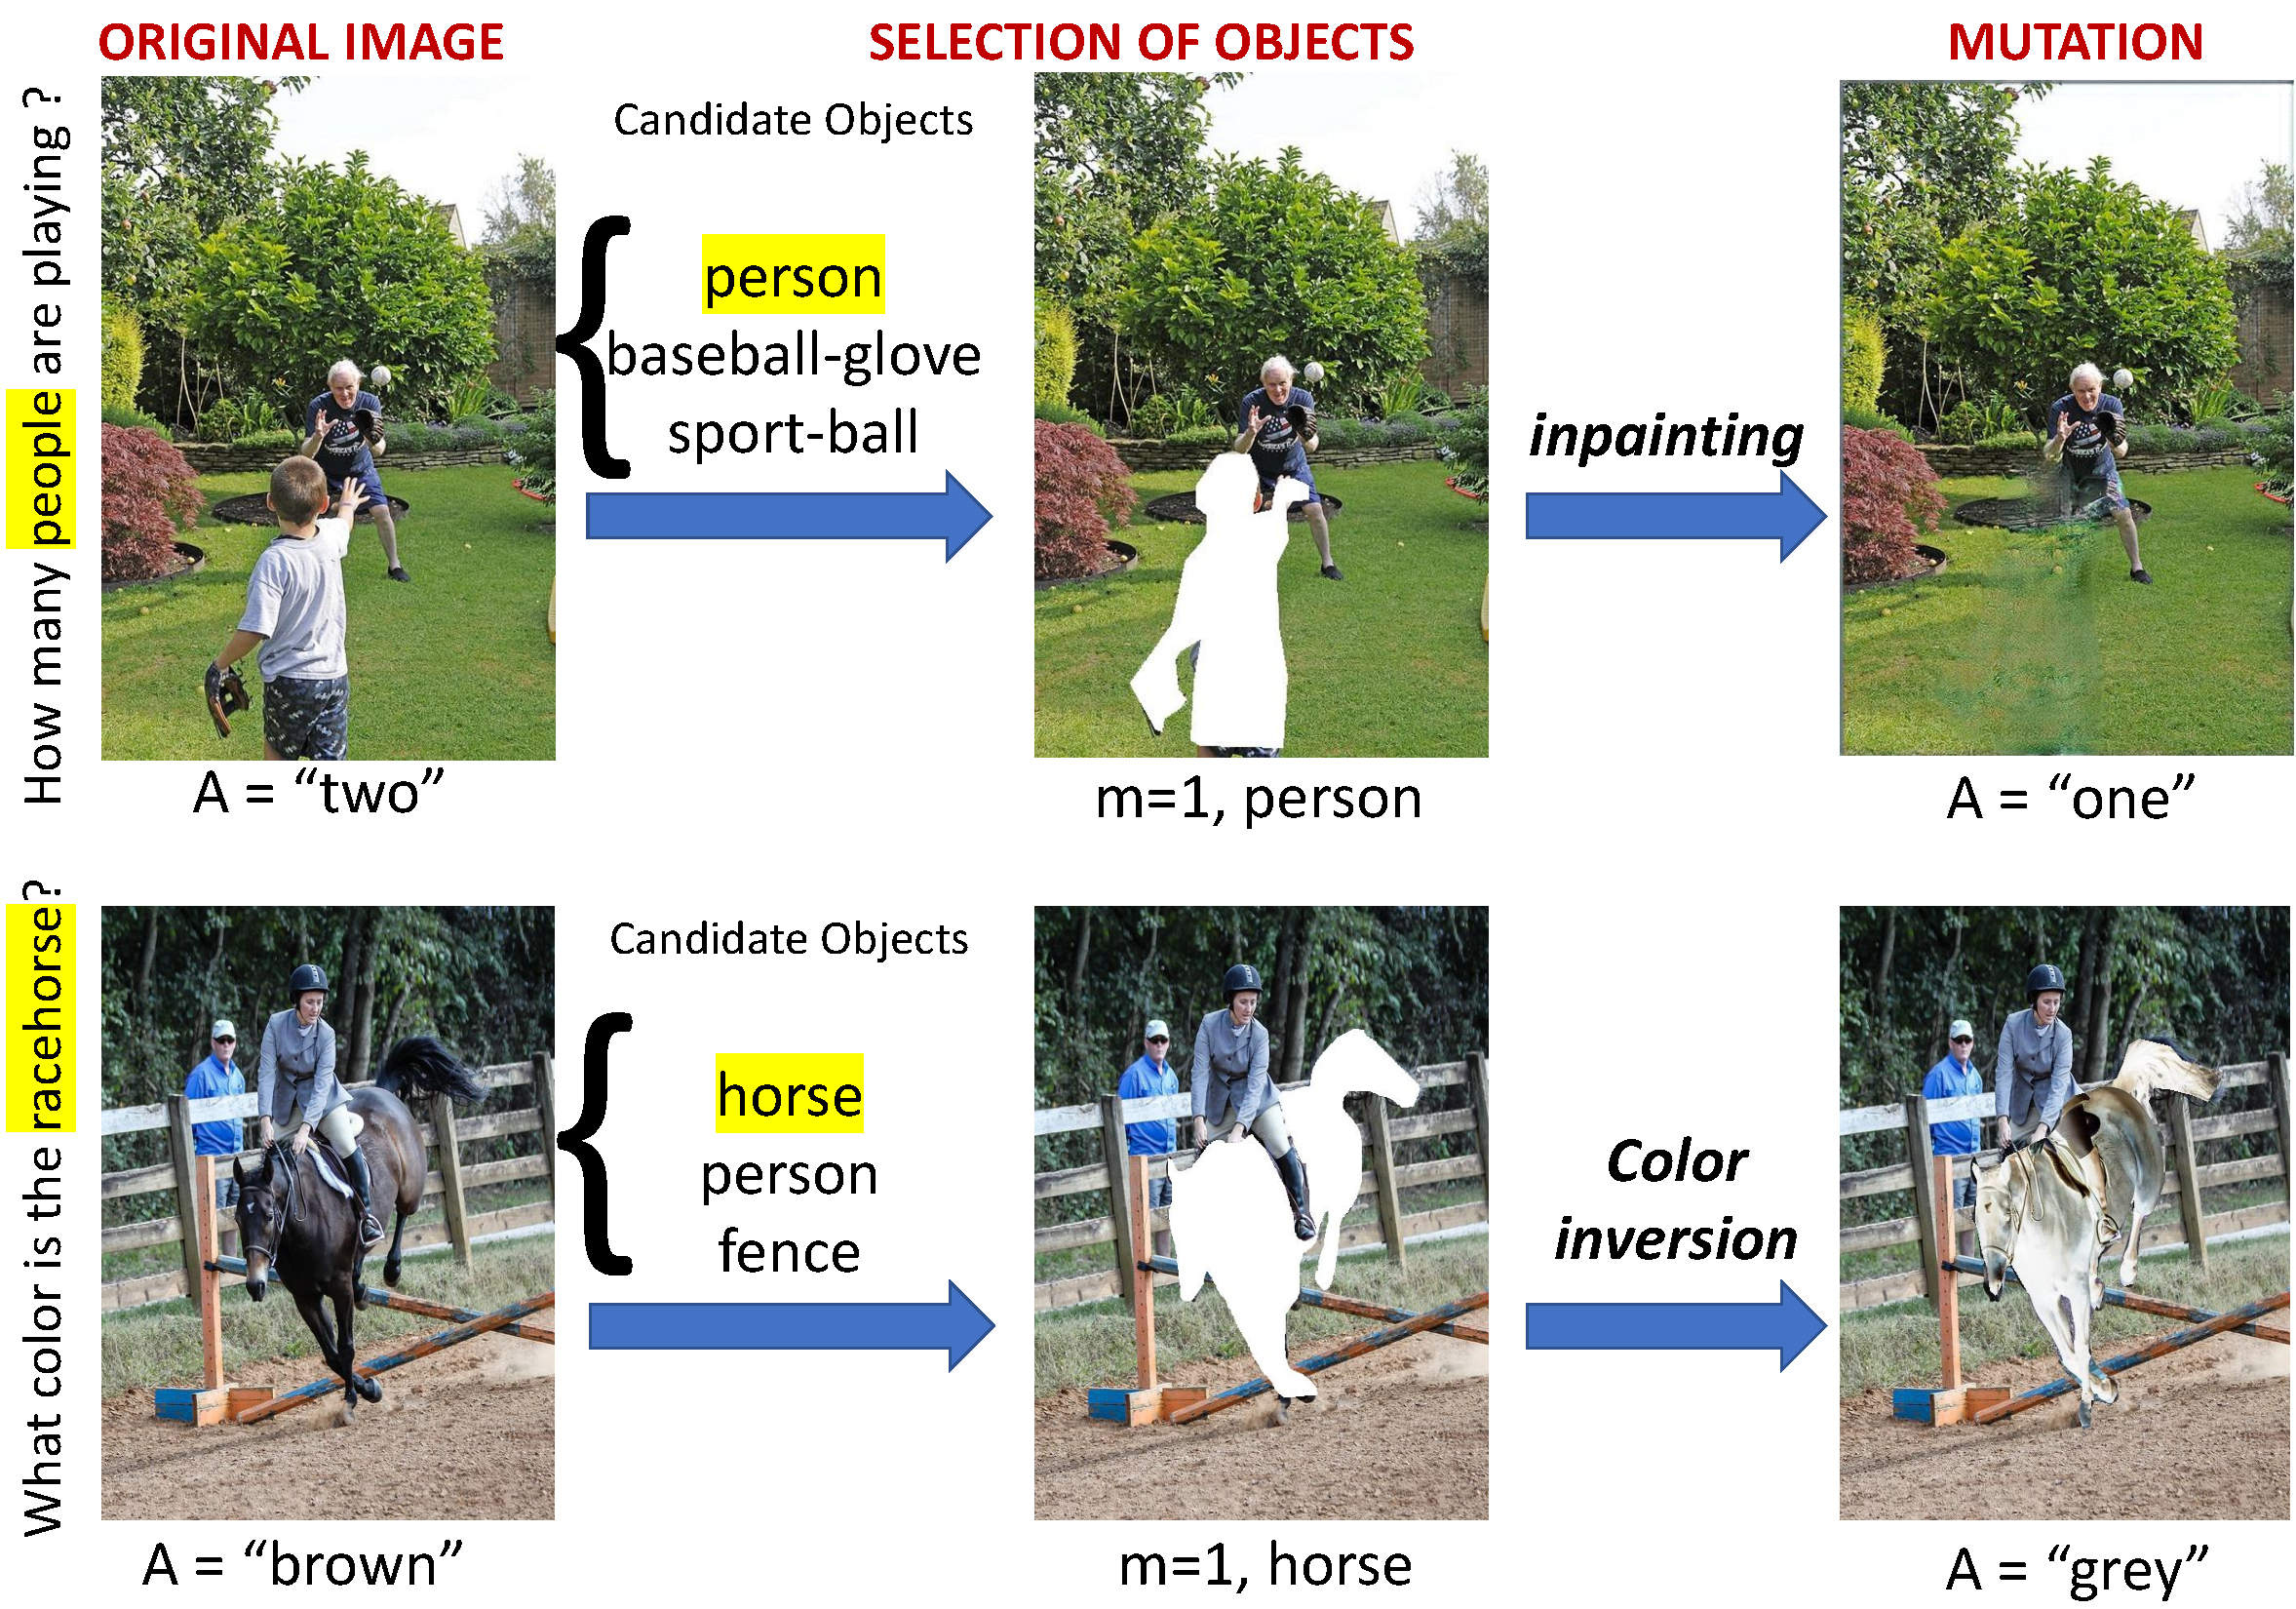
\includegraphics[width=\linewidth]{mutant/figures/mutant_creation.pdf}
    \caption{Figure illustrating our dataset creation pipeline for image mutations.
    $m$ object instances of ``critical" object are identified from the question and image, and mutation performed either by removal or color inversion.
    $A$ represents the answer to the question.}
    \label{fig:image_mutation}
\end{figure}

\begin{figure}
  \begin{minipage}{.31\textwidth}
    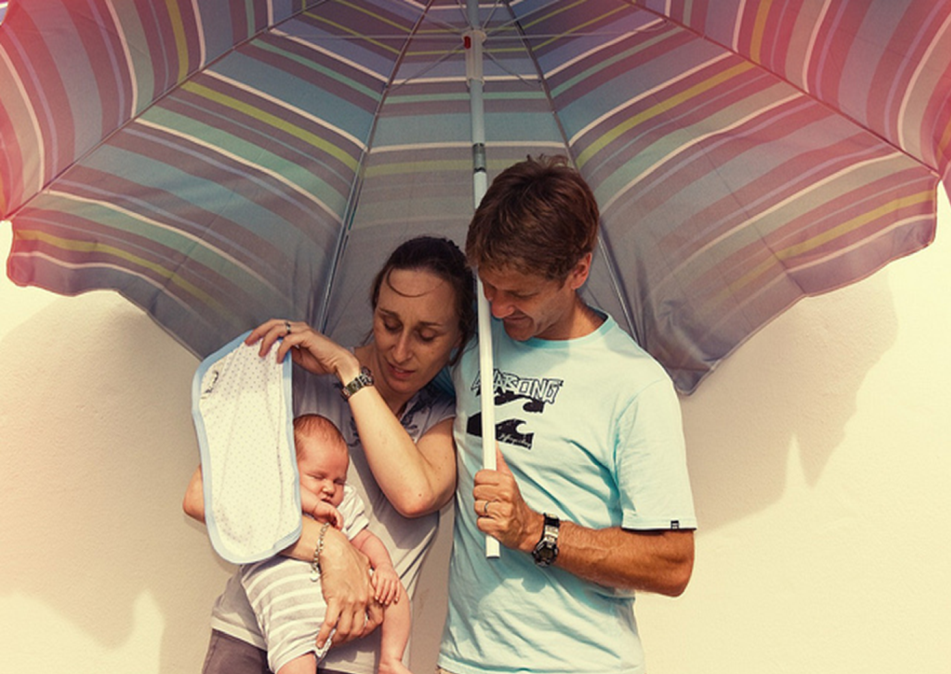
\includegraphics[width=\linewidth]{mutant/figures/lady_lr.png}
  \end{minipage} \quad
  \begin{minipage}{.61\textwidth}
    \resizebox{\linewidth}{!}{
    \begin{tabular}{lll}
        \toprule
        \textbf{Mutation Type} & \textbf{Question} & \textbf{Answer} \\
        \toprule
            Original                    & Is the lady holding the baby?     & Yes \\
            Substitution (Negation)     & Is the lady not holding the baby? & No \\
            Substitution (Adversarial)  & Is the cat holding the baby?      & No \\
            \midrule
            Original & How many people are there? & Three \\
            Deletion (Masking) & How many [MASK] are there? & ``Number"\\
            \midrule
            Original & What is the color of the man's shirt? & Blue \\
            Substitution (Negation) & What is not the color of the man's shirt? & Magenta \\
            \midrule
            
            Deletion (Masking)          & Is the [MASK] holding the baby?   & Can't say \\ 
            \midrule
            Original & What color is the umbrella ? & Pink \\
            Deletion (Masking)          & What color is the [MASK]?   & ``color" \\
        \bottomrule
    \end{tabular}
    }
  \end{minipage}
  \captionof{table}{Examples of our question mutation.
The image is shown on the left, and the original question is in the first row of the table.
Examples of the two types of mutation are shown in the table.}
\label{tab:q_mut}
\end{figure}
    
    


In order to train VQA models under the mutant paradigm, we need a mechanism to create mutant samples.
Mutations are transformations that act on semantic entities in either the image or the question, in ways that can reliably lead to a new answer.
For the question, semantic entities are words, while for images, semantic entities are objects.
It is important to note that our mutation process is automated and does not use the knowledge about the test set distribution in order to create new samples.
In this section, we delineate our automated generation process for both image and question-mutation.


    \subsection{Image Mutations}
    For image mutation, we first identify critical objects from the image that results in a change in the answer, and either remove instances of these objects (removal) or morph their color (substitution).
        
        \paragraph{Removing Object Instances:}
        Removing an instance of an object class can be either critical to the question (i.e. the answer to the question changes) or non-critical (i.e. answer is unchanged).
        If an object (or it's synonym or hypernym) is mentioned in the question, we deem it to be critical to the question, otherwise it is deemed non-critical.
        For each object with $M$ instances in the image, we randomly remove $m$ instances from the image s.t. $m \in \{0, \dots, M\}$ using polygon annotations from the COCO~\citep{lin2014microsoft} dataset.
        Thus for each image, we get multiple masked images, with pixels inside the instance bounding-box removed, as shown in Figure~\ref{fig:image_mutation}.
        These masked images are fed to a GAN-based inpainting network~\citep{yu2018generative} that makes the mutant image photo-realistic, and also prevents the model from getting cues from the shape of the mask. 
        In the case of numeric questions, if $m$ critical objects are removed, the answer to for the mutant image changes from $n$ to $n-m$.
        For yes-no questions, removal of all critical objects ($m=n$) will flip the answer from ``yes" to ``no", while removing $m<n$ critical objects will not.
        Note that $m=0$ corresponds to the original image and does not result in a change in the answer.
        
        \paragraph{Color Inversion:}
        For mutations that involve a change in color, we use samples with questions about the color of objects in the image, and change the color of critical objects by pixel-level color inversion in RGB-space.
        % We identify the critical object in the image and change the color by pixel-level color inversion in RGB-space.
        The true answer is replaced with the new color of the critical objects.
        To get objects with new colors, we do not use the knowledge about colors of objects in the world.
        In some cases, the new colors of the object may not correspond to real-world scenes, thus forcing the model to actually identifying colors, and not answer from language priors, such as ``bananas are yellow".
    
    
    \subsection{Question Mutations}
    We use three types of question mutations as shown in the example in Table~\ref{tab:q_mut}.
    We first identify the critical object and then apply template-based question operators similar to~\citep{gokhale2020vqa}.
    The first operator is negation for yes-no questions, which is achieved by a template based procedure that negates the question by adding a ``no" or ``not" before a verb, preposition or noun phrase.
    The second is the use of antonyms or adversarial object-words to substitute critical words.
    The third mutation masks words in the question and thus introduces ambiguity in the question.
    Questions for which the new answer cannot be deterministically identified are annotated with a broad category label such as \textit{color, location, fruit} instead of the exact answers such as \textit{red, library, apple} which the model cannot be expected to answer since some words have been masked or replaced with adversarial words.
    Yet, we want the model to be able to identify this broad category of answers even under partially occluded inputs.
    The answer remains unchanged for mutations with non-critical objects or words.
    
    % \begin{table*}
%     \centering
%     \resizebox{\linewidth}{!}{
%     \begin{tabular}{| l | l | l | l | l | l |}
%         \hline
%         \textbf{Mutation Category} & Object Removal & Color Change & Negation & Adversarial Substitution & Word Masking \\
%         \hline
%         \textbf{Number of Samples} & 159,899 & 30,759 & 237,611 & 146,814 & 104,666 \\
%          \hline
%     \end{tabular}
%     }
%     \caption{Distribution of generated mutant samples by category of mutation}
%     \label{tab:mutant_stats}
% \end{table*}


\begin{table}
    \centering
    \small
    \begin{tabular}{cc}
        \toprule
        \textbf{Mutation Category} & \textbf{Number of Samples} \\
        \midrule
        Object Removal              & 159,899   \\
        Color Change                & 30,759    \\
        Negation                    & 237,611   \\
        Adversarial Substitution    & 146,814   \\
        Word Masking                & 104,666   \\
        % \textbf{Number of Samples} & 159,899 & 30,759 & 237,611 & 146,814 & 104,666 \\
        \bottomrule
    \end{tabular}

    \caption{Distribution of generated mutant samples by category of mutation}
    \label{tab:mutant_stats}
\end{table}    
    \subsection{Mutant Statistics:}
    We use the training set of VQA-CP-v2~\citep{vqa-cp} to generate mutant samples.
    For each original sample, we generate $1.5$ mutant samples on average, thus obtaining a total of 679k samples.
    Table~\ref{tab:mutant_stats} shows the distribution of our generated mutations with respect to the type of mutation.
    Addition of mutant samples does not change the distribution of samples per question-type.\footnote{More details about mutant samples are in Supp. material.}
    
%     
    % \subsection{Training with Mutants}
    % Our method of training with mutant samples relies on three key concepts that supplement the conventional VQA classification task.
    
    % \paragraph{Answer Projection:}
    
    % \begin{figure*}[t]
    %     \centering
    %     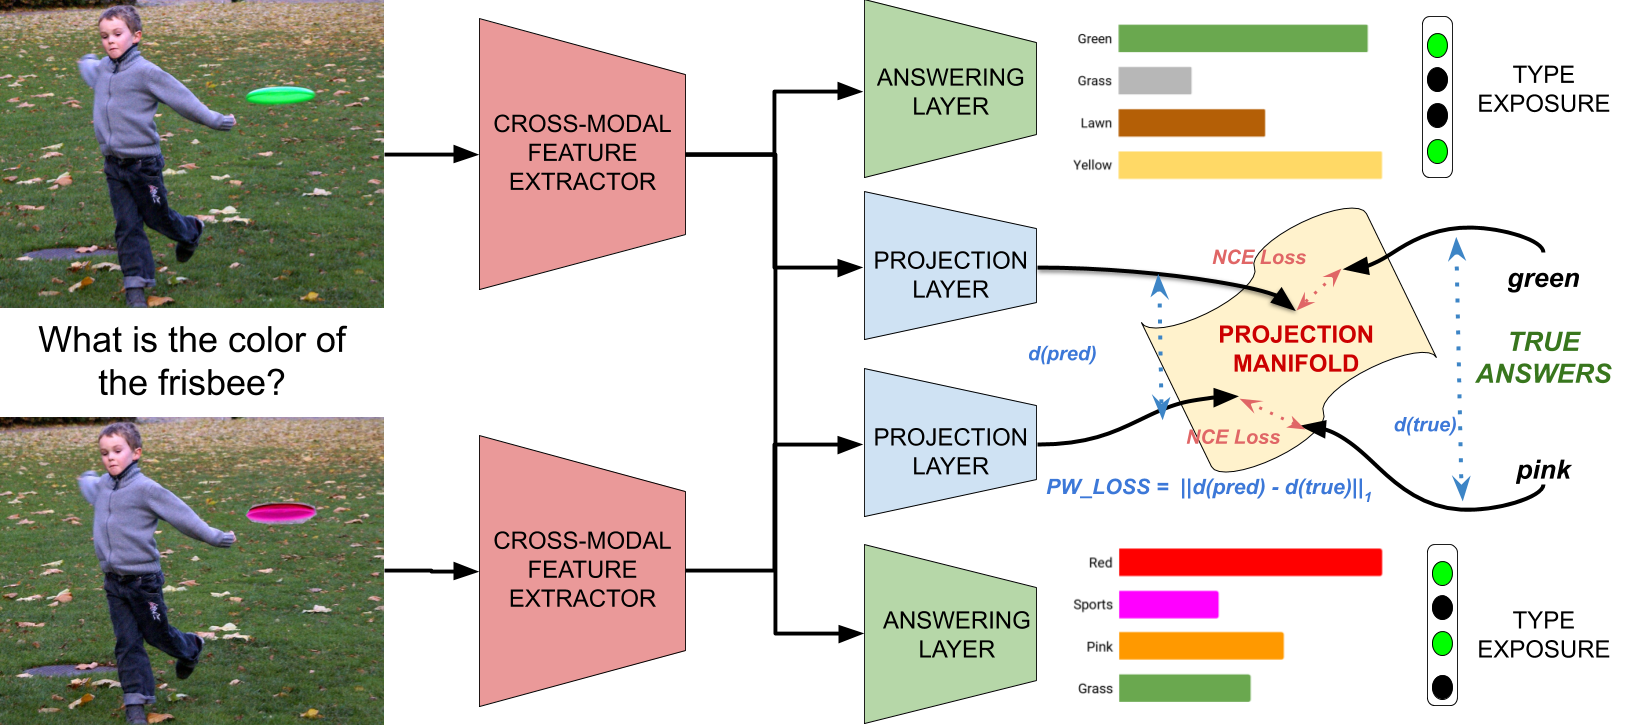
\includegraphics[width=0.9\linewidth]{mutant/figures/overall_final.png}
    %     \caption{Overall architecture of the Mutant Method includes a cross-modal feature extractor, answer projection layer, answering layer and type exposure model}
    %     \label{fig:overall}
    % \end{figure*}
    
    % The traditional learning strategy of VQA models optimizes for a standard classification task using softmax cross-entropy:
    % \begin{equation}
    %     \mathcal{L}_{\scaleto{VQA}{4pt}} = \frac{-1}{N}\sum_{i=1}^{N}\mathit{log}(\mathit{softmax}\big(f_{\mathit{\scaleto{VQA}{4pt}}}(X_i), a_i)).
    % \end{equation}
    % QA as a classification task is popular since the answer vocabulary follows a long-tailed distribution over the dataset.
    % However this formulation is problematic since it does not consider the meaning of the answer while making a decision, but instead learns a correlation between the one-hot vector of the answer-class and input features.
    % Thus to answer the question ``What is the color of the banana", models learn a strong correlation between the question features and the answer-class for ``yellow", but do not encode the notion of \textit{yellowness} or \textit{greenness} of bananas.
    % This key drawback negatively impacts the generalizability of these models to raw green or over-ripe black bananas at test-time.
    
    % To mitigate this, in addition to the classification task, we propose a training objective that operates in the space of answer embeddings.
    % The key idea is to map inputs (image-question pairs) and outputs (answers) to a shared manifold in order to establish a metric of similarity on that manifold.
    % We train a projection layer that learns to project features and answers to the manifold as shown in Figure~\ref{fig:overall}.
    % We then use Noise Contrastive Estimation~\citep{gutmann2010noise} as a loss function to minimize the distance between the projection of cross modal features $z$ and projection of glove vector $v$ for ground-truth answer $\mathit{a}$, given by:
    % \begin{equation}
    %     \mathcal{L}_{\scaleto{NCE}{4pt}} = -log\big(\frac{e^{cos(z_{feat},~~z_{a})}}{\sum_{a_i \in \mathcal{A}} e^{cos(z_{feat},~~z_{a}^i)}}\big),
    % \end{equation} 
    % where $z_{\scaleto{feat}{5pt}} = f_{\scaleto{proj}{5pt}}(z)$ and $z_{a} = f_{\scaleto{proj}{5pt}}(glove(a))$, and $\mathcal{A}$ is the set of all possible answers in our training dataset.
    % It is important to note that this similarity metric is not between the true answer and the predicted answer, but between the projection of input features and the projection of answers, to incorporate context in the answering task.
    
    % \paragraph{Type Exposure:}
    % Linguistic priors in datasets have led models to learn spurious correlations between question and answers. 
    % For instance, in VQA, the most common answer for ``What sport ..." questions is ``tennis", and for ``How many ..." questions is ``two".
    % Our aim is to remove this negative bias from the models.
    % Instead of removing \textit{all bias} from these models, we teach models to identify the question type, and learn which answers can be valid for a particular question type, irrespective of their frequency of occurrence in the dataset.
    % For instance, the answer to ``How many ..." can be all numbers, answers to ``What color ..." can be all colors, and answers to questions such as ``Is the / Are there ..." questions is either yes or no.
    % We call this \textit{Type Exposure} since it instructs the model that although a strong correlation may exist between a question-answer pair, there are other answers which are also valid for the specific type of question.
    % Our Type Exposure model uses a feedforward network to predict question type and to create a binary mask over answer candidates that correspond to this type.
    
    
    % \paragraph{Pairwise-Consistency:}
    % The final component of Mutant is pairwise consistency.
    % We jointly train our models with the original and mutant sample pair, with a loss function that ensures that the distance between two predicted answer vectors is close to the distance between two ground-truth answer vectors.
    % The pairwise consistency loss is given below, where $\mathit{z_a}$ is the vector for answer $\mathit{a}$, $\mathit{m}, GT$ denote mutant sample and ground-truth respectively.
    % \begin{equation}
    %     \mathcal{L}_{\scaleto{PW}{4pt}} = ||cos(z_{a_{GT}}, z_{a_{GT}}^m) - cos(z_{a_{pred}}, z_{a_{pred}}^m)||_1 .
    %     \nonumber
    % \end{equation}
    
    % This pairwise consistency is designed as a regularization that incorporates the notion of semantic shift in answer space as a consequence of a mutation.
    % For instance, consider the image mutation in Figure~\ref{fig:image_mutation} which changes the ground-truth answer from "two" to "one".
    % This shift in answer-space should be reflected by the predictor.
\begin{table}
	\small
	\begin{center}
		\resizebox{\linewidth}{!}{
			\begin{tabular}{@{}l  cccc c cccc c@{}}
				\toprule
				\multirow{2}{*}{Model}  & \multicolumn{4}{c}{VQA-CP v2 test (\%) $\uparrow$} & \hphantom & \multicolumn{4}{c}{VQA-v2 val (\%) $\uparrow$} & \multirow{2}{*}{Gap (\%)}\\
				\cmidrule{2-5} \cmidrule{7-10}
				& All & Yes/No & Num & Other && All & Yes/No & Num & Other & \\
				\toprule
				% HAN~\cite{malinowski2018learning} & 28.65 & 52.25 & 13.79 & 20.33 && - & - & - & - & -\\
				GVQA~\cite{agrawal2018don} & 31.30 & 57.99 & 13.68 & 22.14 && 48.24 & 72.03 & 31.17 & 34.65 & 16.94\\
				AReg~\cite{ramakrishnan2018overcoming} & 41.17 & 65.49 & 15.48 & 35.48 && 62.75 & 79.84 & 42.35 & 55.16 & 21.58\\
				RUBi~\cite{cadene2019rubi} & 47.11 & 68.65 & 20.28 & 43.18 && 63.10 & - & - & - & 14.05 \\ 
				SCR~\cite{wu2019self} & 48.47 & 70.41 & 10.42 & 47.29 && 62.30 & 77.40 & 40.90 & {56.50} & 13.83\\
			    LMH~\cite{clark2019don}  & 52.45 & 69.81 & 44.46 & 45.54 && 61.64 & 77.85 & 40.03 & 55.04 & 9.19\\
				CSS~\cite{chen2020counterfactual}  & 58.95 & 84.37 & 49.42 & 48.21 && 59.91 & 73.25 & 39.77 & 55.11 & {0.96}\\
				
				\midrule
				UpDn~\cite{anderson2018bottom}  & 39.74 & 42.27 & 11.93 & 46.05 && 63.48 & 81.18 & 42.14 & 55.66 & 23.74\\
				% UpDn + Mutant & \\
				UpDn + Ours & 61.72 & 88.90 & 49.68 & 50.78 && 62.56 & 82.07 & 42.52 & 53.28 & 0.84\\
				\midrule
				LXMERT~\cite{tan2019lxmert} & 46.23 & 42.84 & 18.91 & 55.51 && \textbf{74.16} & \textbf{89.31} & \textbf{56.85} & \textbf{65.14} & 27.97\\
				% LXMERT + Mutant  & 59.69 & 73.19 & 32.85 & 59.29\\
				LXMERT + Ours & \textbf{69.52} & \textbf{93.15} & \textbf{67.17} & \textbf{57.78} &&  \underline{70.24} & \underline{89.01} & \underline{54.21} & \underline{59.96} & \textbf{0.72} \\
				\bottomrule
			\end{tabular}
		} % scale box
	\end{center}
	\caption{Accuracies on VQA-CP v2 test and VQA-v2 validation set, along with Percentage gap between overall accuracies on these two datasets. \textit{``Ours"} represents the final model with Answer Projection, Type Exposure and Pairwise Consistency.
	Overall best scores are \textbf{bold}, our best are \underline{underlined.}}
	\label{tab:results}
\end{table}
\section{Experiments}
    \subsection{Setting}
    \paragraph{Datasets:}
    We train and evaluate our models on VQA-CP-v2.
    This is a natural choice for evaluating OOD generalization since VQA-CP is a non-i.i.d.~reorganization of the VQA dataset, and was created in order to evaluate VQA models in a setting where language priors cannot be relied upon for a correct prediction.
    This is because for every question type (65 types according to the question prefix), the prior distribution of answers is different in train and test splits of VQA-CP.
    We also train and evaluate our models on the VQA-v2~\citep{goyal2017making} validation set, and compare the gap between the imbalanced and non-i.i.d.~setting of VQA-CP against the balanced i.i.d.~setting of VQA.
    
    
    \paragraph{Hyperparameters:}
    All of our models are trained on two NVIDIA Tesla V100 16GB GPUs for $10$ epochs with batch size of $32$ and learning rate $1e\text{--}5$.
    Each epoch takes approximately three hours for UpDn and four hours for LXMERT.
    
    
    
    
    \subsection{Baseline Models}
    We compare our method with GVQA~\citep{agrawal2018don}, RUBI~\citep{cadene2019rubi}, SCR~\citep{wu2019self}, LMH~\citep{clark2019don}, CSS~\citep{chen2020counterfactual} as our baselines.
    Since most of these methods are built with UpDn~\citep{anderson2018bottom} as the backbone, we investigate the efficacy of UpDn under the mutant paradigm.
    On the other hand, LXMERT~\citep{tan2019lxmert} has emerged as a powerful transformer-based cross-modal feature extractor, and is pre-trained on tasks such as masked language modeling and cross-modality matching, inspired by BERT~\citep{devlin2018bert}.
    LXMERT is a top performing single-model on multiple vision-and-language tasks such as VQA, GQA~\citep{hudson2019gqa}, ViZWiz~\citep{bigham2010vizwiz}, and NLVR2~\citep{suhr2019corpus}.
    We therefore use is as a strong baseline for our experiments.
    LXMERT is representative of the recent trend towards using BERT-like pre-trained models~\citep{lu2019vilbert,su2019vl,li2020unicoder,chen2019uniter} and fine-tuning them on multiple downstream vision and language tasks.
    Note that we do not use ensemble models for our experiments and focus only on single-model baselines.

    
    \subsection{Results on VQA-CP-v2 and VQA-v2}
    Performance on two benchmarks VQA-CP-v2 and VQA-v2 is shown in Table~\ref{tab:results}.
    We compare existing models against UpDn and LXMERT incorporated into our Mutant method.
    For the VQA-CP benchmark, our method improves the performance of LXMERT by $23.29\%$, thus establishing a new state of the art on VQA-CP, beating the previous best by $10.57\%$.
    Our method shows improvements across all categories, with $8.78\%$ on the Yes-No category, $17.75\%$ on Number-based questions, and $9.57\%$ on other questions.
    We use negation as one of the question mutation operators on yes-no questions, but such questions are not present in the test set.
    However our model takes advantage of this mutation and improves substantially on yes-no questions.
    The Mutant method also consistently improves the performance of the UpDn model by $21.98\%$ overall.
    Note that baseline models AReg, RUBI, SCR, LMH, and CSS all modify UpDn by adding de-biasing techniques. 
    We show our de-biasing method improves on two SOTA models and outperforms all of the above baselines, unlike previous work which only modifies UpDn.
    This empirically shows Mutant to be model-agnostic.
    % paradigm.
    
    When trained and evaluated on the balanced i.i.d.~VQA-v2 dataset, our method achieves the best performance amongst methods designed specifically for OOD generalization, with an accuracy of $70.24\%$.
    This is closest among baselines to the SOTA established by LXMERT, which is trained explicitly for the balanced, i.i.d.~setting.
    To make this point clear, we report the \textit{gap} between the overall scores for VQA-CP and VQA-v2, following the protocol from~\citet{chen2020counterfactual} in Table~\ref{tab:results}.
    
    % \paragraph{Results on VQA-v2 without re-training:}
    % Additionally, we use our best model trained on VQA-CP and evaluate it on the VQA test standard set without re-training on VQA-v2 data.
    % The objective here is to evaluate whether models trained on biased data (VQA-CP) and mutant data is able to generalize to VQA-v2 which uses an i.i.d. train-test split.
    % This gives us an overall accuracy of $67.63\%$ comprising with $88.56\%$ on yes-no questions, $50.76\%$ on number-based questions, and $54.56\%$ on other questions.
    % This is better than all existing VQA-CP models that are explicitly trained on VQA-v2 (reported in Table~\ref{tab:results}), and thus demonstrates the generalizability of our approach.
    
    
    
    

    
    % \subsection{Analysis}
    % \begin{table}
    \centering
    \resizebox{\linewidth}{!}{
    \begin{tabular}{@{}p{1.75cm}>{\RaggedRight}p{3.45cm} p{0.7cm}p{0.7cm}p{0.7cm}p{0.7cm}}
        \toprule 
        \multirow{2}{*}{Model} & \multirow{2}{*}{Data} & \multicolumn{4}{c}{VQA-CP v2 test $\uparrow$ (\%)}\\
        \cmidrule{3-6}
        & & All & Yes/No & Num & Other \\
        \toprule
        UpDn    & VQA-CP            & 39.74 & 42.27 & 11.93 & 46.05 \\
        UpDn    & VQA-CP + Mutant   & 50.16 & 61.45 & 35.87 & 50.14 \\
        \hdashline
        \multicolumn{2}{c}{\textit{Increase in Accuracy}} & \textit{10.42} & \textit{19.18} & \textit{23.94} & \textit{4.09}\\
        \hdashline
        LXMERT  & VQA-CP            & 46.23 & 42.84 & 18.91 & 55.51 \\
        LXMERT  & VQA-CP + Mutant   & 59.69 & 73.19 & 32.85 & 59.29 \\
        \hdashline
        \multicolumn{2}{c}{\textit{Increase in Accuracy}} & \textit{13.46} & \textit{30.35} & \textit{13.94} & \textit{3.78}\\
        \midrule 
        LXM~+~Ours & VQA-CP + Img. Mut. & 64.85 & 85.68 & 66.44 & 53.80\\
        LXM~+~Ours & VQA-CP + Que. Mut. & 67.92 & 91.64 & 65.73 & 56.09\\
        LXM~+~Ours & VQA-CP + Both Mut. & \textbf{69.52} & \textbf{93.15} & \textbf{67.17} & \textbf{57.78} \\
        \bottomrule
    \end{tabular}
    }
    \caption{Top section: Comparison of UpDn and LXMERT when trained on VQA-CP and augmented with mutant samples, and the increase in accuracy due to mutant samples.
    Bottom section: Comparison of LXMERT when using image or text mutations, or both.}
    \label{tab:effect_data}
\end{table}
    % \begin{table}
    \centering
    \resizebox{\linewidth}{!}{
    \begin{tabular}{@{}lcccc@{}}
        \toprule 
        \multirow{2}{*}{Model} & \multicolumn{4}{c}{VQA-CP v2 test $\uparrow$ (\%)}\\
        \cmidrule{2-5}
        & All & Yes/No & Num & Other \\
        \toprule
        UpDn                    & 50.16 & 61.45 & 35.87 & 50.14 \\
        UpDn~+~AP             &  54.51 & 88.35 & 41.01 & 32.89\\
        UpDn~+~TE             &  56.32 & 80.56 & 46.14 & 46.41\\
        UpDn~+~AP~+~TE       &  55.76 & 90.25 & 43.78 & 41.40\\
        UpDn~+~AP~+~PW         &  57.54 & 91.59 & 49.17 & 41.93\\
        UpDn~+~TE~+~PW        &  60.32 & 86.10 & 50.23 & 49.58 \\
        UpDn~+~AP~+~TE~+~PW  &  61.72 & 88.90 & 49.68 & 50.78\\
        \midrule
        LXM                  & 59.69 & 73.19 & 32.85 & 59.29 \\
        LXM~+~AP            & 60.45 & 88.46 & 43.24 & 50.49 \\
        LXM~+~TE           & 63.36 & 77.10 & 46.50 & 61.27 \\
        LXM~+~AP~+~TE     & 64.73 & 85.34 & 47.23 & 58.71 \\
        LXM~+~AP~+~PW       & 67.14 & 90.49 & 65.52 & 55.34 \\
        LXM~+~TE~+~PW      & 64.17 & 94.71 & 35.19 & 48.80 \\
        LXM~+~AP~+~TE~+~PW & \textbf{69.52} & \textbf{93.15} & \textbf{67.17} & \textbf{57.78} \\
        
        \bottomrule
    \end{tabular}
    }
    \caption{Ablation study to investigate the effect of each component of our method: Answer Projection (AP), Type Exposure (TE), Pairwise Consistency (PW), and independent effect of image and question mutations.}
    \label{tab:ablation}
\end{table}
    
        
    %     \paragraph{Effect of Training with Mutant Samples:\\}
    %     In this analysis we measure the effect of augmenting the training data with mutant samples on UpDn and LXMERT without any architectural changes.
    %     The results are reported in Table~\ref{tab:effect_data}.
    %     Both models improve when exposed to the mutant samples, UpDn by $10.42\%$ and LXMERT by $13.46\%$.
    %     There is a markedly significant jump in performance for both models for the yes-no and number categories.
    %     UpDn especially benefits from Mutant samples in terms of the accuracy on numeric questions (a boost of $23.94\%$).
        
    %     We also compare our final model when trained only with image mutations and only with question mutations in Table~\ref{tab:effect_data}.
    %     While this is worse than training with both types of mutations, it can be seen that question mutations are better than image mutations in the case of yes-no and other questions, while image mutations are better on numeric questions.
        
    %     \paragraph{Ablation Study:\\}
    %     We conduct ablation studies to evaluate the efficacy of each component of our method, namely Answer Projection, Type Exposure and Pairwise Consistency, on both baselines, as shown in Table~\ref{tab:ablation}.
    %     Introduction of Answer Projection significantly improves yes-no performance, while Type Exposure improves performance on other questions.
    %     We also observe that the pairwise consistency loss significantly boosts performance on numeric questions and yes-no questions.
    %     Note that there is a minor difference between the original and the mutant sample, and the model needs to understand this difference, which in turn can enable the model to reason about the question and predict the new answer.
    %     For instance the pairwise consistency loss allows the model to learn the correlation between one missing object and a change in answer from ``two" to ``one" in Figure~\ref{fig:image_mutation}, resulting in an improvement in the counting ability of our VQA model.
    %     Similarly, the pairwise consistency allows the model to improve on yes-no questions for which the answer changes when a critical object is removed.
        
    %     \begin{table}
    \centering
    \resizebox{\linewidth}{!}{
    \begin{tabular}{@{}p{2.65cm}p{1.1cm}cccc@{}}
        \toprule 
        \multirow{2}{*}{Model} & \multirow{2}{*}{Method} & \multicolumn{4}{c}{VQA-CP v2 test $\uparrow$ (\%)}\\
        \cmidrule{3-6}
        & & All & Yes/No & Num & Other \\
        \toprule
        UpDn + Ours    & Base   & 61.72 & 88.90 & 49.68 & 50.78 \\
        UpDn + Ours    & LMH    & 55.38 & 90.99 & 39.74 & 40.99 \\
        \hdashline
        \multicolumn{2}{c}{\textit{Drop in Accuracy}} & \textit{6.34} & \textit{-2.09} & \textit{9.95} & \textit{9.80}\\
        \midrule
        LXMERT + Ours & Base    & 69.52 & 93.16 & 67.17 & 57.78 \\
        LXMERT + Ours & LMH     & 63.85 & 88.34 & 48.23 & 55.28\\
        \hdashline
        \multicolumn{2}{c}{\textit{Drop in Accuracy}} & \textit{5.67} & \textit{4.82} & \textit{18.86} & \textit{2.50} \\
        \bottomrule
    \end{tabular}
    }
    \caption{Effect of combining LMH de-biasing with the Mutant paradigm, measured as drop in accuracy (\%)}
    \label{tab:lmh}
\end{table}
    %     \paragraph{Effect of LMH Debiasing on Mutant:\\}
    %     We compare the results of our model when trained with or without the explicit de-biasing method LMH~\citep{clark2019don}.
    %     LMH is an ensemble-based method trained for \textit{avoiding} dataset biases, and is the most effective among all de-biasing strategies developed for the VQA-CP challenge.
    %     LMH implements a learned mixing strategy, by using the main model in combination with a bias-only model trained only with the question, without the image.
    %     The learned mixing strategy uses the bias-only model to remove biases from the main model.
    %     It can be seen from Table~\ref{tab:lmh} that LMH leads to a drop in performance when used in combination with Mutant.
    %     This is potentially because in the process of debiasing, LMH ends up attenuating positive bias introduced by Mutant that is useful for generalization.
    %     \citet{kervadec2020roses} have concurrently shown that de-biasing methods such as LMH indeed result in a decrease in performance on out-of-distribution (OOD) test samples in the GQA~\citep{hudson2019gqa} dataset, mirroring our analysis on VQA-CP shown in Table~\ref{tab:lmh}.
        


% %%%%%%%%%%%%%%%%%%%%%%%%%%%%%%%%%%%%%%%%%%%%%%%%%%%%%%%%%%%%%%%%
% % RELATED WORK
% %%%%%%%%%%%%%%%%%%%%%%%%%%%%%%%%%%%%%%%%%%%%%%%%%%%%%%%%%%%%%%%%
% \section{Related Work} 

%     \paragraph{De-biasing of VQA datasets:}
%     The VQA-v1 dataset~\citep{antol2015vqa} contained imbalances and language priors between question- answer pairs.
%     This was mitigated by VQA-v2~\citep{goyal2017making} which balanced the data by collecting complementary images such that each question was associated with two images leading to two different answers.
%     Identifying that the distribution of answers in the VQA dataset led models to learn superficial correlations,~\citet{vqa-cp} proposed the VQA-CP dataset by re-organizing the train and test splits such that the the distribution of answers per question-type was significantly different for each split.


%     \paragraph{Robustness in VQA:}
%     Ongoing efforts seek to build robust VQA models for VQA for various aspects of robustness.
%     \citet{shah2019cycle} propose a model that uses cycle-consistency to not only answer the question, but also generate a complimentary question with the same answer, in order to increase the linguistic diversity of questions. 
%     In constrast, our work generates questions with a different answer.
%     \citet{selvaraju2020squinting} provide a dataset which contains perception-related sub-questions for each VQA question.
%     Antonym-consistency has been tackled in~\citet{ray2019sunny}.
%     Inspired by invariant risk minimization~\citep{arjovsky2019invariant} which links out-of-distribution generalization to invariance and causality,~\citet{teney2020unshuffling} provide a method to identify invariant correlations in the training set and train models to ignore spurious correlations.
%     \citet{asai2020logic,gokhale2020vqa} explore robustness to logical transformation of questions using first-order logic connectives \textit{and} ($\wedge$), \textit{or} ($\vee$), \textit{not} ($\neg$).
%     Removal of bias has been a focus of ~\citet{ramakrishnan2018overcoming,clark2019don} for the VQA-CP task.
%     We distinguish our work from these by amplifying positive bias and attenuating negative bias.
    
%     \paragraph{Data Augmentation:}
%     It is important to note that the above work on data de-biasing and robust models focuses on the language priors in VQA, but not much attention has been given to visual priors.
%     Within the last year, there has been interest in augmenting VQA training data with counterfactual images~\citep{agarwal2020towards,chen2020counterfactual}. Independently,~\citet{teney2020learning} have also demonstrated that counterfactual images obtained via minimal editing such as masking or inpainting can lead to improved OOD generalization of VQA models, when trained with a pairwise gradient-based regularization.
%     Self-supervised data augmentation has been explored in recent work~\citep{lewis-etal-2019-unsupervised,fabbri2020template,banerjee2020self} in the domain of text-based question answering.
%     The mutant paradigm presented in this work is one of the first enable the generation of VQA samples that result in different answers, coupled with a novel architecture and a consistency loss between original and mutant samples as a training objective. 
    
    
%     \paragraph{Answer Embeddings:}
%     In one of the early works on VQA,~\citet{teney2016zero} use a combination of image and question representations and answer embeddings to predict the final answer. 
%     \citet{hu2018learning} learn two embedding functions that transform image-question pair and answers to a shared latent space.
%      Our method is different from this since we use a combination of classification and NCE Loss on the projection of answer vectors, as opposed to a single training objective.
%     This means that although the predicted answer is obtained as the most probable answer from a set of candidate answers, the NCE Loss in the answer-space embeds the notion of semantic similarity between the answer.
%     Our Type Exposure model is in principal similar to~\citet{kafle2016answer} who use the predicted answer-type probabilities in a Bayesian framework, while we use it as an additional constraint, i.e. as a regularization for a maximum likelihood objective.


%%%%%%%%%%%%%%%%%%%%%%%%%%%%%%%%%%%%%%%%%%%%%%%%%%%%%%%%%%%%%%%%
% DISCUSSION
%%%%%%%%%%%%%%%%%%%%%%%%%%%%%%%%%%%%%%%%%%%%%%%%%%%%%%%%%%%%%%%%
\section{Discussion}
In this paper, we present a method that uses input mutations to train VQA models with the goal of Out-of-Distribution generalization.
% Our novel answer projection module trained for minimizing distance between answer and input projections complements the canonical VQA classification task.
% Our Type Exposure model allows our network to consider all valid answers per question type as equally probable answer candidates, thus moving away from the negative question-answer linguistic priors.
% Coupled with pairwise consistency, these modules achieve a new state-of-the-art accuracy on the VQA-CP-v2 dataset and reduce the gap between model performance on VQA-v2 data.
We differentiate our work from methods using random adversarial perturbations for robust learning~\citep{madry2018towards}.
Instead we view input mutations as \textit{structured perturbations} which lead to a semantic change in the input space and a deterministic change in the output space.
We envision that the concept of input mutations can be extended to other vision and language tasks for robustness.
% Concurrent work in the domain of image classification shows that carefully designed perturbations or manipulations of the input can benefit generalization and lead to performance improvements~\citep{chen2020simple,hendrycks2019augmix}.
% While perception is a cornerstone of understanding, the ability to imagine changes in the scene or language query, and predict outputs for that \textit{imagined} input allows models to supplement ``what" decision making (based on observed inputs) with ``what if" decision making (based on imagined inputs), and this work falls in the la
% The Mutant paradigm is an effort towards ``what if" decision making. 



\chapter{Semantically Distributed Robust Optimization for Vision and Language Inference} 
\label{chap:sdro}
% \begin{abstract}
% Analysis of vision-and-language models has revealed their brittleness under linguistic phenomena such as paraphrasing, negation, textual entailment, and word substitutions with synonyms or antonyms.
% While data augmentation techniques have been designed to mitigate against these failure modes, methods that can integrate this knowledge into the training pipeline remain under-explored.
% In this paper, we present \textbf{SDRO},
% \footnote{Code and data will be released upon publication.}
% % \footnote{\href{https://github.com/ASU-APG/VLI_SDRO}{\footnotesize\url{https://github.com/ASU-APG/VLI_SDRO}}}, 
% a model-agnostic method that utilizes a set linguistic transformations in a distributed robust optimization setting, along with
% an ensembling technique to leverage these transformations during inference.
% Experiments on benchmark datasets with images (NLVR$^2$) and video (VIOLIN) demonstrate performance improvements as well as robustness to adversarial attacks.
% Experiments on binary VQA explore the generalizability of this method to other V\&L tasks.

% \end{abstract}
%-------------------------------------------------------------------------
%%%%%%%%% INTRODUCTION
% \section{Introduction}
\label{sec:01_intro}
\textit{``Does the text match the image?''} -- this simple question represents the Vision-and-Language Inference (VLI) task,
as shown in Figure~\ref{fig:example_vli}.
Image-text matching forms the backbone for V\&L pre-training~\citep{sun2019videobert,tan2019lxmert,lu2019vilbert,chen2020uniter} and has resulted in improvements in downstream tasks such as visual question answering, image retrieval, referring expressions, and visual commonsense reasoning.
While Natural Language Inference (without visual inputs) has been extensively studied~\citep{bowman2015large,williams2018broad,khot2018scitail,demszky2018transforming}, VLI demands the additional capability of being grounded in the scene while understanding semantics.
Although pre-trained language models (PLMs)~\citep{vaswani2017attention,devlin2019bert,raffel2020exploring} have been useful for encoding text into vector embeddings, recent findings point to undesirably high cosine similarity of two random words~\citep{ethayarajh2019contextual}, the struggle with negation~\citep{kassner2020negated,ettinger2020bert}, and semantically equivalent adversarial examples~\citep{ribeiro2018semantically}.
These findings call for robust training protocols to avoid propagation of these findings into VLI models.
\begin{figure}
    \centering
    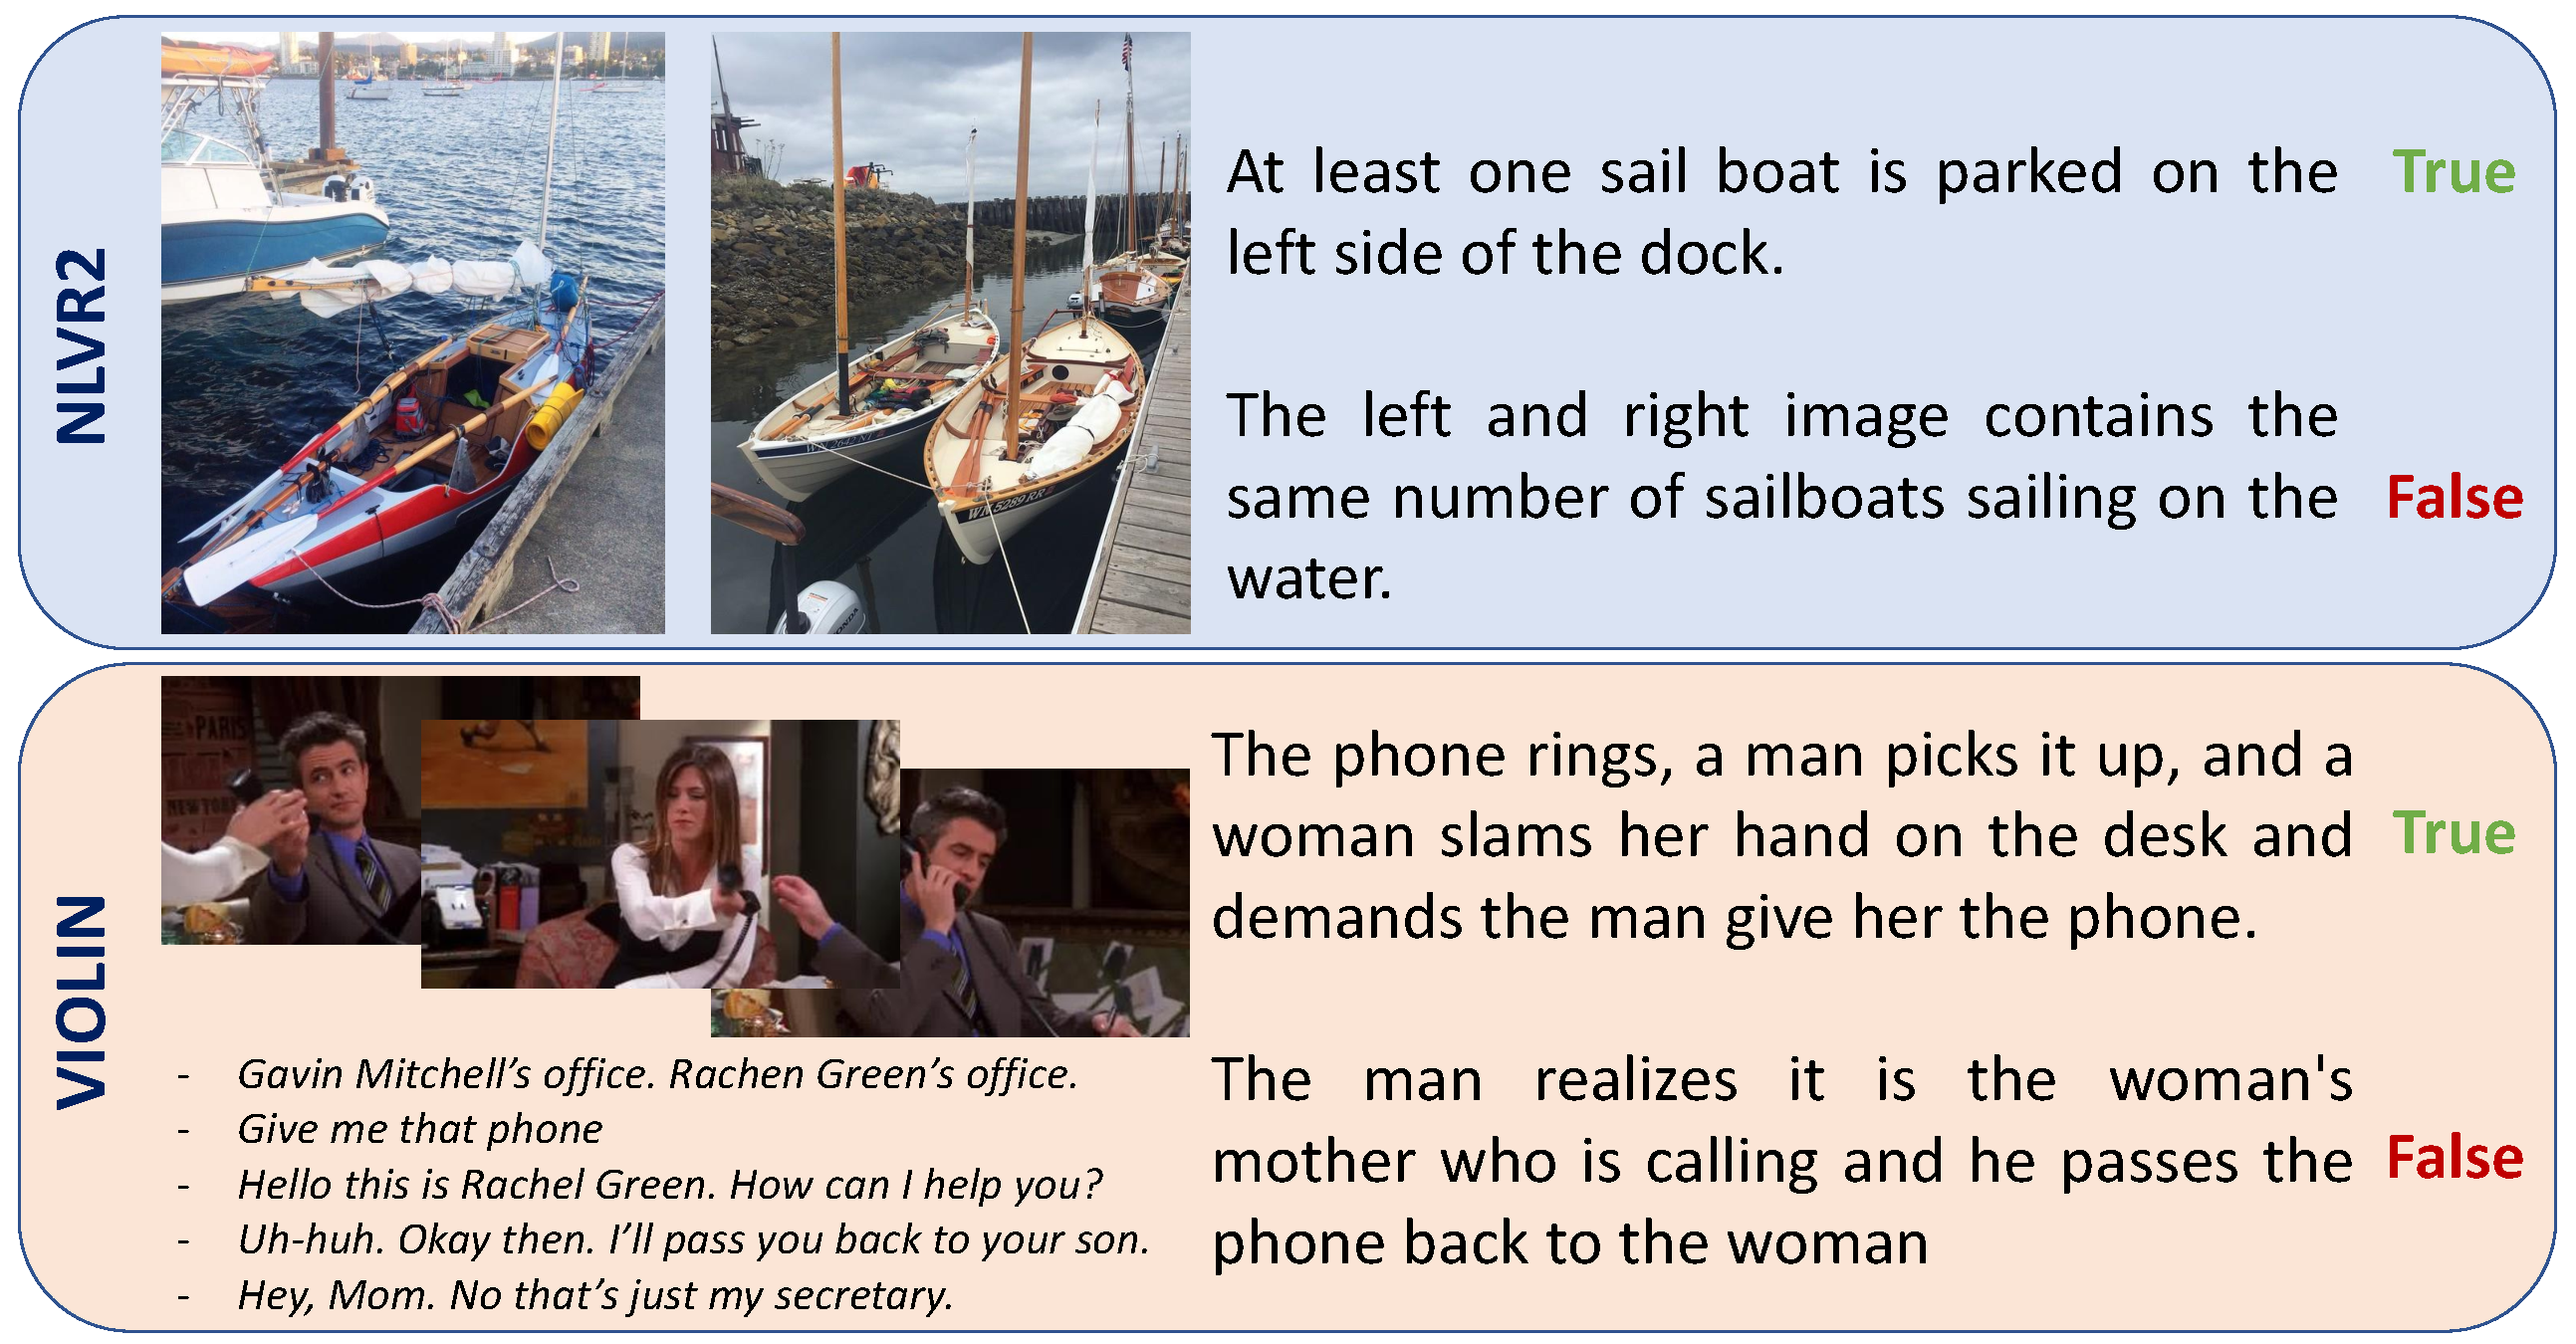
\includegraphics[width=\linewidth]{sdro/images/example_nlvr_violin.pdf}
    \caption{
        VLI models predict whether a sentence is \texttt{True} or \texttt{False} about the visual input. \textit{(Top)} sample from NLVR$^2$ with two images as input; \textit{(bottom)} sample from VIOLIN with video and subtitles as input.
        }
    \label{fig:example_vli}
\end{figure}


Adversarial training (AT) and distributed robust optimization (DRO)~\citep{madry2018towards,hu2018does,sinha2017certifying} have emerged as effective solutions to related problems in robust image classification, such as adversarial defense and domain generalization~\citep{volpi2018generalizing}.
DRO assumes a perturbation set (typically an $\ell_p$ norm ball) around the training distribution, and minimizes the worst-case performance over this perturbation set.
AT and DRO are popular for computer vision tasks, since the small perturbations of pixel intensities do not change the categorical meaning of the image.

However, in the case of text inputs, even small perturbations of their vector embeddings may result in absurd sentences or vectors that do not map to any word-token in vocabulary. 
The topology of the PLM embedding space is not well understood, especially with regard to what kind (and magnitude) of perturbations result in specific changes in semantics, such as similar meanings (speak $\rightarrow$ talk) or opposite meanings (Heaven $\rightarrow$ Hell) without resulting in random or absurd words.
We therefore argue that vector-based additive perturbations present limitations in the case of text inputs.
However, in the domain of natural language, we are blessed with semantic and logical transformations as shown in Table~\ref{tab:sisp_examples}.
This enables linguistically-informed perturbations with control over the semantics of the resulting sentence and label, as shown in Figure~\ref{fig:vector_vs_linguistic}.

\begin{figure}
    \centering
    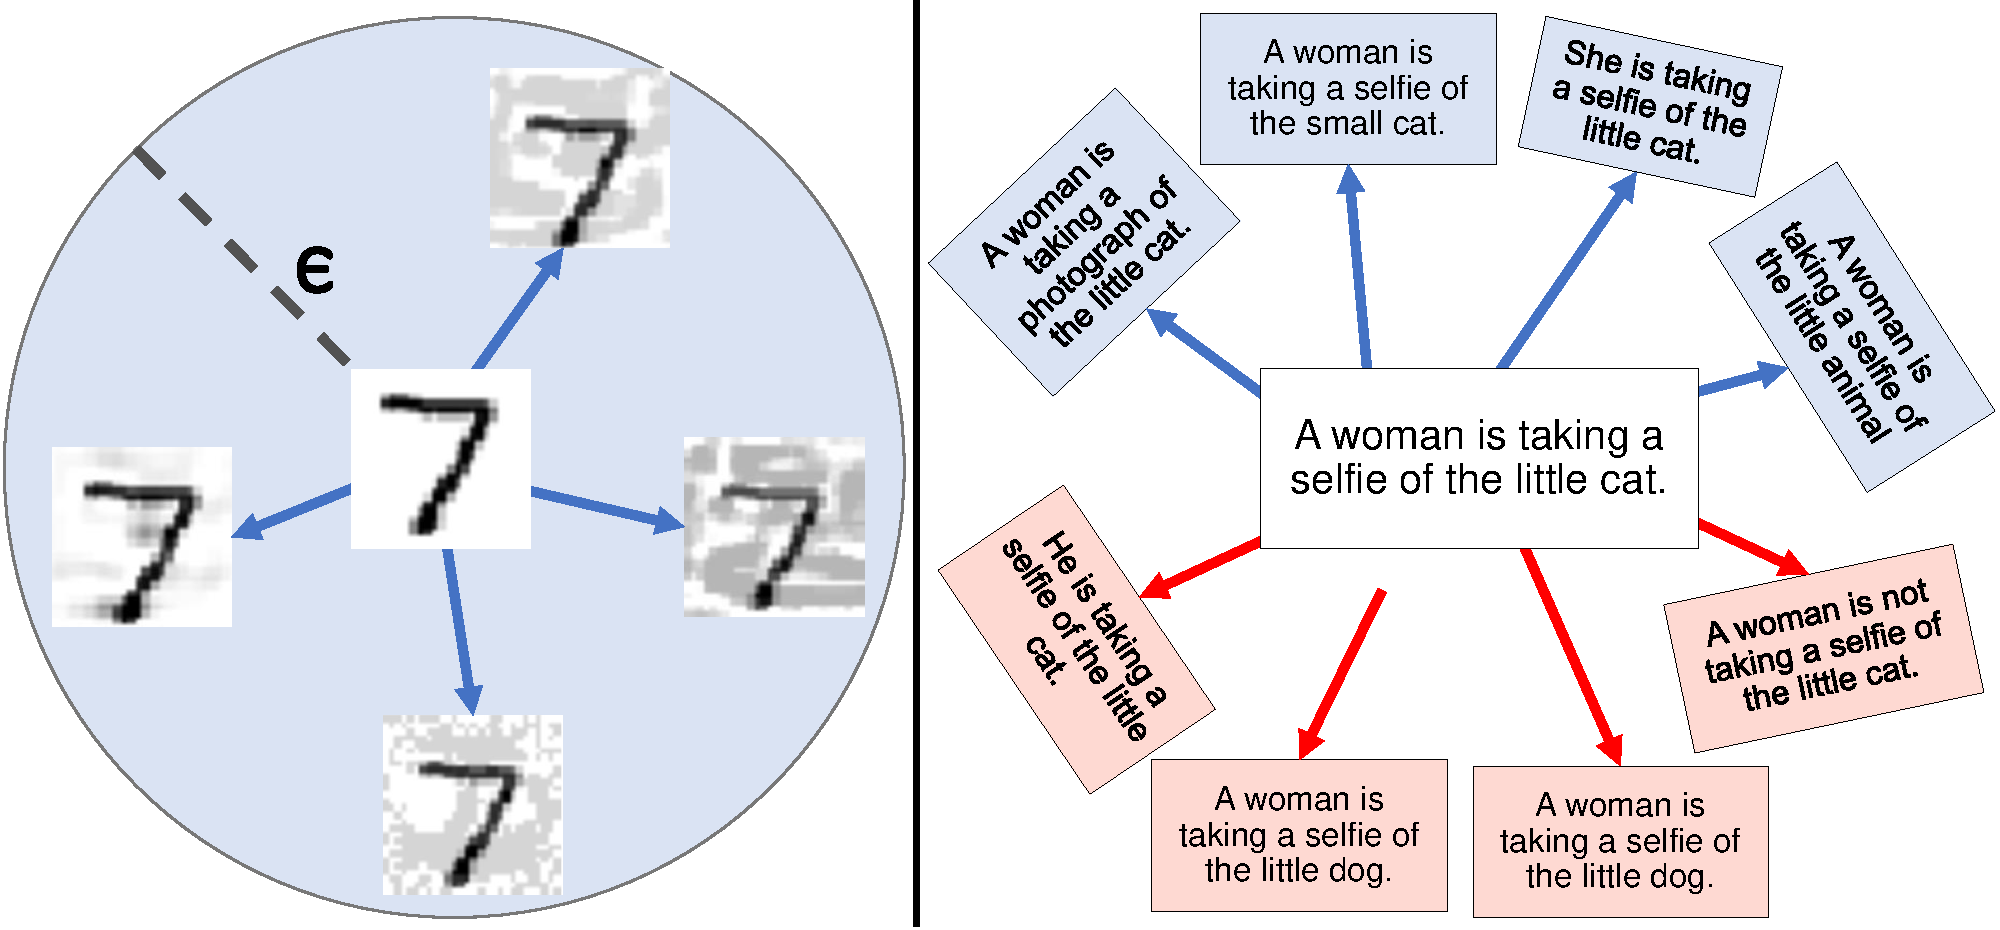
\includegraphics[width=0.95\linewidth]{sdro/images/vector_vs_linguistic.pdf}
    \caption{
    Comparison between \textit{(left)}
    \straightepsilon-bounded image perturbations and \textit{(right)} linguistics-based \textit{Semantics-preserving} (blue) as well as  \textit{Semantics-Inverting} (red) transformations for sentences.
    }
    \label{fig:vector_vs_linguistic}
\end{figure}
    
We present a technique that modifies robust optimization by incorporating linguistically-informed transformations.
Our approach: \textbf{S}emantically \textbf{D}istributed \textbf{R}obust \textbf{O}ptimization (SDRO) 
utilizes a pre-defined set of linguistic transformations (such as negation, word substitution, and paraphrasing) as the perturbation set instead of optimizing over the vector-space.
We dub this set of transformations ``SISP'' i.e., semantics-inverting (SI) and semantics-preserving (SP) transformations.
SDRO is \textit{model-agnostic} since it can be applied to text inputs of any existing VLI model and \textit{dataset agnostic} since it uses automated transformations without explicit knowledge of the text domain.

We apply SDRO to two VLI benchmark datasets: image-based NLVR$^2$~\citep{suhr2019corpus} as well as video-based VIOLIN~\citep{liu2020violin}.
To demonstrate the generalizability of SDRO to other V\&L tasks, we also report results on the ``yes/no'' subset of VQA-v2~\citep{goyal2017making}.
Our experiments show model-agnostic improvements in accuracy for all three benchmarks.
While models trained with naive data augmentation using SISP suffer from a trade-off between robustness and accuracy, models that utilize SDRO improve along both metrics.
SDRO also allows us to learn in low-resource settings, serving as a smart data augmentation tool -- SDRO models trained only with $80\%$ of the original dataset outperform existing state-of-the-art which utilizes the entire dataset.

Since SISP transforms do not require the true label to either produce an SP or SI transformed sentence, we can apply them at test-time.
Given a test input sentence, we generate its SISP versions and ensemble the predictions made by the model, giving equal weight to the prediction for the original sentence and the average predictions for all transformed sentences.
We find that this ensembling of predictions of the SDRO model at test-time pushes the state-of-the-art further, thereby demonstrating the usefulness of semantic sentence transformations, both during training and testing.

%-------------------------------------------------------------------------
%%%%%%%%% SDRO
\section{Method} 
\begin{table}
    \centering
    % \small
    \resizebox{\linewidth}{!}{
    \begin{tabular}{@{}clp{0.425\linewidth}p{0.425\linewidth}@{}}
        \toprule
         & \textbf{Category}    & \textbf{Original} & \textbf{Transformed} \\
        \toprule 
        \multirow{6}{*}{\rotatebox{90}{SI}}
         & Noun-Antonym
            & The two women are driving on the street with the convertible top down.
            & The two \textit{\textbf{men}} are driving on the street with the convertible top down.\\
         & Verb-Antonym
            & There are children standing by the door.
            & There are children \textbf{\textbf{sitting}} by the door.\\
         & Comparative-Antonym
            & There are more monitors in the image on the right than on the left.
            & There are \textit{\textbf{few}} monitors in the image on the right than on the left. \\
         & Number-Substitution
            & There are three bowls of dough with only one spatula.
            & There are \textit{\textbf{eleven}} bowls of dough with only one spatula. \\
         & Pronoun-Substitution 
            & In one of the images, a woman is taking a selfie. 
            & In one of the images, \textit{\textbf{he}} is taking a selfie.\\
         & Subject-Object Swap
            & The two women are driving on the street with the convertible top down. 
            & The two \textit{\textbf{top}} are driving on the street with the convertible \textit{\textbf{women}} down.\\
         & Negation
            & The closet doors on the right are mirrored.
            & The closet doors on the right are \textit{\textbf{not}} mirrored\\
        \midrule
        \multirow{6}{*}{\rotatebox{90}{\footnotesize SP}}
         & Noun-Synonym         
            & The right image shows three bottles of beer lined up.
            & The right \textit{\textbf{picture}} shows three bottles of beer lined up.\\
         & Verb-Synonym         
            & Someone is using a kitchen utensil
            & Someone is \textit{\textbf{utilizing}} a kitchen utensil. \\
         & Comparative-Synonym  
            & The bottle on the right is larger than the bottle on the left.
            & The bottle on the right is \textit{\textbf{bigger}} than the bottle on the left.\\
         & Number-Substitution  
            & The two white swans are swimming in the canal gracefully. 
            & The \textit{\textbf{less than seven}} white swans are swimming in the canal gracefully.\\ 
         & Pronoun-Substitution 
            & In one of the images, a woman is taking a selfie. 
            & In one of the images, \textit{\textbf{she}} is taking a selfie.\\
         & Paraphrasing         
            & A man in a green shirt came on the porch and knocked on the door.
            & A man in a green shirt came \textit{\textbf{up to}} the porch and knocked on the door. \\
        \bottomrule 
    \end{tabular}
    }
    \caption{Illustrative examples for the effect of each SISP transformation on input sentences.}
    \label{tab:sisp_examples}
\end{table}

\subsection{Preliminaries}
Consider a training distribution $P_{tr}$ consisting of inputs $\x$ and labels $\y$.
For VLI, input $\x$ is multi-modal (visuals and text), with labels $\y \in \{\texttt{True}, \texttt{False}\}$.
Under the empirical risk minimization (ERM), the following risk is minimized:
\begin{equation}
    \mathcal{R}_{ERM} = \E_{(\x, \y) \sim P_{tr}}  ~\ell(f(\x; \theta), \y).
    \label{sdro:eq:erm}
\end{equation}
ERM provides generalization guarantees~\citep{vapnik1991principles} for i.i.d.\ test samples, but not for out-of-distribution or adversarial examples.

\paragraph{Distributed Robust Optimization (DRO)}~\citep{pmlr-v80-hu18a,sagawa2020distributionally} searches for loss-maximizing perturbations of the input within an $\epsilon$-divergence ball around $P_{tr}$ and minimize the risk over such perturbed distributions.
\begin{equation}
    \mathcal{R}_{DRO}=\underset{P:D(P, P_{tr})<\epsilon}{sup}\E_{(\x, \y) \sim P} \ell(f(\x; \theta), \y).
    \label{sdro:eq:std_adv}
\end{equation}
The solution to Equation~\ref{sdro:eq:std_adv} guarantees robustness inside such $\epsilon$-bounded distributions $P$.
The inner maximization is typically solved using gradient-based methods~\citep{madry2018towards} over additive perturbations $\delta$ such that $\x+\delta$ fools the classifier.


\subsection{SDRO}
\label{sec:sdro}
For sentence inputs, additive perturbations are intangible and may result in ambiguity.
An alternative approach is to consider \textit{groups} or perturbations sets $\mathcal{G}$ representing certain subpopulations or semantic categories within the data distribution.
For text inputs, we consider perturbation sets that can be created using semantic sentence transformations such as those shown in Table~\ref{tab:sisp_examples}, as the \textit{groups} (or equivalently, \textit{transformations}).
These transformations $g(x, y) = (\x_g, \y_g)$ are of two types:
semantics-preserving (SP) if $\y_g{=}\y$, or semantics-inverting (SI) if $\y_g \neq \y$.
The ability of generating adversarial samples with inverted meanings is a key distinction between adversarial training (AT) and SDRO.
While AT is restricted to SP perturbations inside an $\epsilon$ norm-ball, SDRO can impart larger linguistic perturbations (both SI and SP) beyond the norm-ball, by minimizing the worst-case expected risk over these groups:
\begin{equation}
    \mathcal{R}_{SDRO} = \underset{g\in\mathcal{G}}{sup}\E_{(\x, \y) \sim g} ~\ell(f(\x; \theta), \y).
    \label{sdro:eq:sdro}
\end{equation}


\paragraph{Implementation.}
As a first step of SDRO, we randomly sample a subset $\mathcal{C}$ of the training dataset $\mathcal{D}$ s.t. $|\mathcal{C}|/|\mathcal{D}|=T$. 
We find adversarial samples after every epoch and create an augmented dataset $\mathcal{D}_{aug}$ which contains $(1-T)|\mathcal{D}|$ original samples and $T|\mathcal{D}|$ adversarial samples, thus retaining the size of the training dataset.
We define $\ell_g$ as the classification loss for a transformed sample $(\x_g, \y_g)$:
\begin{equation}
    \ell_g(\x, \y) \triangleq \ell(f(\x_g), \y_g),~\forall g{\in}\mathcal{G}.
    \label{sdro:eq:ell_G}
\end{equation}
We design two variants of SDRO: Sample-Wise (SW) and Group-Wise (GW).
\paragraph{Sample-Wise SDRO:}
    In this greedy version of SDRO, for every input $\x$, a transformation that maximally fools the classifier: $g^*{=}\argmax_{g\in\mathcal{G}} \ell_g(\x, \y)$, is added to the set of adversarial examples $\mathcal{D}_{adv}$. The model is then fine-tuned on the augmented dataset.
    \begin{align}
        \mathcal{D}_{adv} &= \{ g^*(\x, \y) \colon (\x, \y){\in}~\mathcal{C}\}, \\
        \mathcal{D}_{aug} &= \mathcal{D}_{1:(1-T)|\mathcal{D}|} \cup \mathcal{D}_{adv}
        \label{sdro:eq:d_aug}
    \end{align}
    However, this greedy approach is susceptible to the model's biases towards certain transformations.  
    For instance, if negation and verb-antonym are universally hard for most sentences, i.e., result in the maximum classifier loss amongst all  transformations $g$, then $\mathcal{D}_{adv}$ will be dominated by these groups, resulting in an unbalanced training set.
    
\paragraph{Group-Wise SDRO}
is devised to mitigate against the model becoming biased towards the ``hardest'' transformations.
    Using Equation~\ref{sdro:eq:ell_G}, we calculate the transformation losses for each transformation of each sample in a training batch, yielding a set of classifier losses per ``group'' $g$:
    \begin{equation}
        L_g \colon \mathcal{C} \rightarrow \R;
        ~L_g = \{ \ell_g(\x, \y) \colon (\x, \y) \in \mathcal{C}\}.
    \end{equation}
    We obtain the top-k losses per group $g$ as:
    \begin{equation}
        L_G^k = \argmax_{\Lambda \subset L_G, |\Lambda| = k} \sum_{\lambda\in\Lambda} \lambda,
        ~~\text{where~}k = \floor*{\frac{|\mathcal{C}|}{|\mathcal{G}|}}.
        \label{sdro:eq:pergroup_losses}
    \end{equation}
    Then 
    $\mathcal{D}_{adv}$ is compiled as the union of per-group adversaries using Equation~\ref{sdro:eq:pergroup_losses}, and augmented to the training dataset using Equation~\ref{sdro:eq:d_aug}.
    
\paragraph{Test-Time Ensembling of Predictions.}
Semantic transformations $g$ allow us to obtain multiple ``views'' $\x_g = g(\x)$ of the input, and the corresponding predictions $\hat{\y}_g = f(\x_g)$.
We ensemble these predictions and the original prediction $\hat{\y}=f(\x)$ with a simple weighted-average.
Note that $\mathcal{G}$ contains both SP and SI transformations, $\mathcal{G}_{SP}$ and $\mathcal{G}_{SI}$. 
Since the expected label for $\mathcal{G}_{SI}$ is flipped, during ensembling we use the flipped probabilities $1{-}f(\x_g)$.
The ensembled prediction is:
\begin{equation}
\hat{\y}_{e} = \alpha f(\x) +
\frac{1{-}\alpha}{2}\sum_{\mathclap{g\in\mathcal{G}_{SP}}}{\frac{f(\x_g)}{|\mathcal{G}_{SP}|}} + \frac{1{-}\alpha}{2}\sum_{\mathclap{g\in\mathcal{G}_{SI}}}\frac{1{-}f(\x_g)}{|\mathcal{G}_{SI}|}.
\label{sdro:eq:ensembling}
\end{equation}
This ensembling is in principle similar to~\citet{chai2021ensembling} who train a generative model $g$ to output different views of an image, and tune $\alpha$ over a validation set.
In our work, $g$ are semantic sentence transformations, and a simple intuitive choice of $\alpha{=}0.5$ gives equal weight to the original sample and the SISP versions.
We find that:
\begin{enumerate}[nosep,noitemsep,leftmargin=*]
\item training models with SDRO using SISP transformations improves results on VLI tasks, and
\item ensembling predictions of SDRO at test-time using Equation~\ref{sdro:eq:ensembling} further improves results.
\end{enumerate}
%-------------------------------------------------------------------------
\section{SISP Sentence Transformations}
This section describes the generation of semantics-preserving (SP) and semantics-inverting (SI) statements.
\textbf{SISP} transforms are implemented using Spacy~\citep{spacy}.
Dataset statistics and additional visualizations are in the Appendix.

\noindent \textbf{Noun Synonym/Antonym:}
We extract nouns (subjects and objects) with dependency parsing, and find two nearest (synonyms) or farthest (antonyms) neighbors in the GloVe space~\citep{pennington2014glove} using a threshold of $0.55$.

\noindent \textbf{Verb Synonym/Antonym:}
We extract verbs using POS tagging and obtain their synonyms or antonyms.
Verbs are lemmatized and inflected to the correct form using Lemminflect~\citep{lemminflect}.

\noindent \textbf{Comparative Synonym/Antonym:}
Adjectival complements and modifiers are replaced with synonyms (\textit{large $\rightarrow$ big}) or antonyms (\textit{large $\rightarrow$ small}). 

\noindent \textbf{Number Substitution:}
Numerals are replaced by number-words (2 $\rightarrow$ \textit{two}) or vice versa for SP transformations, or by their lower or upper bounds,
(SP: \textit{3 $\rightarrow$ more than two}, SI: \textit{two $\rightarrow$ less than two}).

\noindent \textbf{Pronoun Substitution:}
Human-related nouns (such as \textit{woman, boy, people}) are substituted by pronouns, while pronouns are substituted by generic descriptors (\textit{something, someone, somebody, they}).

\noindent \textbf{Negation:}
We use template-based negation~\citep{gokhale2020vqa} with Subject-Verb Agreement~\citep{wren2000english}.
We add \textit{`did not'} before a past-tense verb, \textit{`do not'}, \textit{`does not'}, or \textit{`not'} before a base-form verb, gerund, or participle, or a \textit{`not'} before an adposition or adjective.

\noindent \textbf{Subject-Object Swap:}
Nominal or clausal subjects and direct or prepositional objects from the sentence are swapped for inverting semantics.

\noindent \textbf{Paraphrasing:}
Input sentences are translated to Russian and then back-translated to English using neural machine translation~\citep{ott2019fairseq}.

\subsection{Data Analysis}
\label{sec:sisp_fidelity_bias}
\paragraph{Quantification of Bias:}
\begin{table}
    \centering
    % \footnotesize
    % \resizebox{\linewidth}{!}{
    \begin{tabular}{@{}l ccc c ccc@{}}
        \toprule
        \multirow{2}{*}{\textbf{Method}} & \multicolumn{3}{c}{NLVR2} & \hphantom & \multicolumn{3}{c}{VIOLIN} \\ 
         \cmidrule{2-4} \cmidrule{6-8}
         & Clean & SP & SI && Clean & SP & SI \\
         \midrule 
        Data-Aug & 51.07 & 50.92 & 40.74 && 61.12 & 62.78 & 62.15 \\
        SW-SDRO  & 51.14 & 50.97 & 40.75 && 62.78 & 58.13 & 64.78 \\
        GW-SDRO  & 51.07 & 50.92 & 40.73 && 62.15 & 52.79 & 74.98 \\
        \bottomrule
    \end{tabular}
    % }
    \caption{Text-only evaluation of biases due to SISP transformations. $50\%$ indicates no bias.}
    \label{tab:eval_textonly_bias}
\end{table}
Since SISP transforms are based on templates, they can potentially introduce spurious linguistic correlations in the dataset.
For example, in NLVR$^2$ and VIOLIN datasets, negations and indefinite pronouns
are infrequent.
To quantify how this could impact models, we mask out the entire image and evaluate models (with VILLA as the backbone for NLVR$^2$ and HERO for VIOLIN).
This acts as a `text-only' evaluation, with accuracies ${\sim}50\%$ implying lesser bias since models do not have access to visual information.
Table~\ref{tab:eval_textonly_bias} shows that SP transforms inflict lesser bias on models than SI transforms.
The effect of bias is dataset-specific; SI makes the prediction of NLVR$^2$ samples harder than random (less than $50\%$ accuracy) but easier for VIOLIN.\\


\noindent\textbf{Transformation Fidelity:}
We employ human subjects to evaluate the quality of SISP-transformed sentences on (1) correctness of labels, (2) grammar, (3) semantics, and (4) visual grounding. 
We report a unified average `transformation fidelity' (details are in Appendix).
Fidelity is higher for SP samples than SI ($90.50\%$ v/s $79.51\%$), which resonates with the complexities of inversion of meaning~\citep{russell1905denoting} and leaves room for improvement in SI transformation.
Although some level of ambiguity exists in SISP transforms, our results show that SDRO models benefit from transformed data.


%-------------------------------------------------------------------------
%%%%%%%%% EXPERIMENTS
\section{Experiments}
\paragraph{Datasets.}
For all datasets, given images/videos and natural language text as input, the system is expected to predict a binary class label.
NLVR$^2$~\citep{suhr2019corpus} contains ${\sim}86K, 7K, 7K$ samples for training, development, and testing respectively.
Each sample in NLVR$^2$ consists of a pair of images (from search engines) and a sentence (crowd-sourced).
VIOLIN~\citep{liu2020violin} contains video clips from popular TV shows and movies along with subtitles and crowd-sourced statements.
VIOLIN contains $76K$, $9.5K$, $9.5K$ samples for training, validation and testing.
VQA Yes/No consists of image-question-answer triplets from VQA-v2 dataset~\citep{goyal2017making}.
While VQA-v2 consists of multiple question and answer types, we focus on the subset of questions with binary \textit{yes/no} answers (${\sim}38\%$ of VQA-v2).
    
\paragraph{Evaluation Metrics.}
We use two evaluation metrics:
(1) \textbf{Clean Accuracy}: accuracy on the i.i.d.\ benchmark test set, and
(2) \textbf{SISP Accuracy}: average performance on SISP transformations of the test set.
Since SISP transformations are automated and can be noisy (Sec~\ref{sec:sisp_fidelity_bias}), evaluation on the SISP test set can be considered a proxy for robustness.

\footnotetext[3]{
Notation: \textbf{bold}: higher than SOTA;
shaded: higher than respective backbone;
\uline{underlined}: best SI/SP accuracies.
}

\subsection{Results}
We compare SDRO with backbone models that use standard training data \textit{(BASE)} and data-augmentation \textit{($+$data-aug)}.
We train SDRO and backbones with the same hyperparameters.
We apply test-time ensembling to the best SDRO model.
\paragraph{NLVR$^2$:}
\input{sdro/tables/results_NLVR2}
We use Transformer-based models LXMERT~\citep{tan2019lxmert}, UNITER~\citep{chen2020uniter}, and VILLA~\citep{gan2020large} as backbones for SDRO. 
VILLA (the current state-of-the-art for NLVR$^2$) uses standard adversarial training.
The percentage of SISP-transformed samples is fixed at $T{=}20\%$.
Table~\ref{tab:results_nlvr2} shows results on the NLVR$^2$ test set, with consistent model-agnostic improvements in clean accuracy over each baseline model and improved robustness on average.
Both variants of SDRO improve over VILLA$_{BASE}$ by $0.84\%$ and $1.02\%$, respectively.
Test-time ensembling using Equation~\ref{sdro:eq:ensembling} leads to further gains, resulting in a new state-of-the-art accuracy of $82.22\%$, an improvement of $3.83\%$ over VILLA$_{BASE}$.
GW-SDRO results in the highest SI accuracy when used with each backbone model.



\paragraph{VIOLIN:}
\begin{table}
    \centering
    % \footnotesize
    % \resizebox{0.9\linewidth}{!}{
    \begin{tabular}{@{}lcccc@{}}
        \toprule
        \multirow{2}{*}{\textbf{Model}} & \multirow{2}{*}{\textbf{Clean Acc.}} & \multicolumn{3}{c}{\textbf{SISP Acc.}} \\
        \cmidrule{3-5}
         &  & SP & SI & Avg. \\
        \midrule
        VIOLIN$_{BASE}$              & 68.07 & 57.17 & 57.20 & 57.18 \\           
        \qquad + data-aug            & 61.58 & \textul{67.64} & 67.70 & 67.67 \\
        \qquad + SW-SDRO             & 62.81 & 62.84 & 62.68 & 62.76 \\
        \qquad + GW-SDRO             & 63.71 & 64.58 & 63.16 & 63.87 \\
        \qquad \qquad + Ensemble     & 66.56 & --''-- & --''-- & --''-- \\
        \midrule
        HERO$_{BASE}$               & 68.55 & 65.59 & 32.00 & 48.80 \\
        \qquad + data-aug            & 65.21 & 59.20 & 81.81 & \textul{70.51} \\
        \qquad + SW-SDRO    & \cellcolor{VeryLightGray}{\textbf{68.83}} & 58.97 & 77.83 & 68.41 \\
        \qquad + GW-SDRO             & 68.19 & 56.20 & \textul{82.92} & 69.57 \\
        \qquad \qquad + Ensemble     & \cellcolor{VeryLightGray}{\textbf{69.90}} & --''-- & --''-- & --''-- \\
        \bottomrule
    \end{tabular}
    % }
    \caption[Results on VIOLIN test set.]{Results on VIOLIN.\footnotemark[\value{footnote}]}
    \label{tab:results_violin}
\end{table}
We consider VIOLIN$_{BASE}$~\citep{liu2020violin} and HERO~\citep{li2020hero}, the current state of the art, as baselines.
VIOLIN$_{BASE}$ separately computes visual features using Faster-RCNN~\citep{ren2015faster} and textual features using BERT~\citep{devlin2019bert}, and fuses them to be used as input to a classifier model.
On the other-hand, HERO is a large-scale transformer-based pre-trained model which uses various V\&L pre-training tasks to compute cross-modal features.
We set $T{=}40\%$.
The results can be seen in Table~\ref{tab:results_violin}.
SW-SDRO model with the HERO backbone improves the state-of-the-art to $68.83\%$, and test-time ensembling further improves it to $69.90\%$. 
Interestingly, similar improvements in clean accuracy are not observed for VIOLIN$_{BASE}$, potentially because it does not use cross-modal pre-trained features.

\paragraph{VQA Yes/No:}
\begin{table}
    \centering
    % \resizebox{0.9\linewidth}{!}{
    \begin{tabular}{@{}lcccc@{}}
        \toprule
        \multirow{2}{*}{\textbf{Model}} & \multirow{2}{*}{\textbf{Clean Acc.}} & \multicolumn{3}{c}{\textbf{SISP Acc.}} \\
        \cmidrule{3-5}
         &  & SP & SI & Avg. \\
        \midrule
        % % LXMERT (all data)           & 86.65 & 75.41 & 34.09 & 54.75\\
        % LXMERT\footnote{LXMERT and UNITER follow a different train-val split}                      & 82.71 & 75.53 & 33.32 & 53.92\\
        % LXMERT\footnotemark[1] + LOL                & 84.75 & 73.77 & 42.97 & 58.37 \\
        % LXMERT-VILLA              & {83.85} & 76.70 & 34.68 & 55.59 \\
        % \midrule
        UNITER$_{BASE}$             & 83.49 & 72.04 & 38.90 & 55.47 \\
        \qquad + data-aug           & 82.53 & 77.03 & 93.70 & 85.36 \\
        \qquad + SW-SDRO    & \cellcolor{VeryLightGray}{83.92} & 75.82 & 88.92 & 81.48 \\ 
        \qquad + GW-SDRO     & \cellcolor{VeryLightGray}{84.05} & 76.95 & 93.41 & 85.18 \\
        \qquad \qquad + Ensemble     & \cellcolor{VeryLightGray}{84.22} & --''-- & --''-- & --''-- \\
        \midrule
        VILLA$_{BASE}$              & 84.82 & 74.15 & 37.40 & 55.77 \\
        \qquad + data-aug            & 83.54 & \textul{78.33} & \textul{94.55} & \textul{86.45} \\
        \qquad + SW-SDRO    & 84.54 & 74.02 & 88.32 & 81.17 \\
        \qquad + GW-SDRO     & \textbf{\cellcolor{VeryLightGray}{{85.12}}} & 77.92 & 93.42 & 85.67 \\
        \qquad \qquad + Ensemble     & \cellcolor{VeryLightGray}{\textbf{85.37}} & --''-- & --''-- & --''-- \\
        \bottomrule
    \end{tabular}
    % }
    \caption[Results on the VQA yes/no subset.
    Not to be compared with VQA-v2 leaderboard since we use a smaller training set.]{Results on the VQA yes/no subset.\footnotemark[\value{footnote}] Not to be compared with VQA-v2 leaderboard since we use a smaller training set of \textit{yes/no} questions.
    % Note that these results should not be compared with VQA-v2 leaderboard since we use a smaller training set.
    }
    \label{tab:results_vqayesno}
\end{table}
We use UNITER and VILLA as the backbone models, with $T{=}20\%$.
The motivation behind VQA experiments is to show that SISP transforms and SDRO can be extended to other V\&L tasks.
Table~\ref{tab:results_vqayesno} shows that GW-SDRO is the best performing model in terms of clean accuracy, and is further improved by test-time ensembling.



%-------------------------------------------------------------------------
%%%%%%%%% ANALYSIS
\section{Analysis}
\label{sec:05_analysis}

\subsection{Visualization of Perturbations}
\begin{figure}
    \centering
    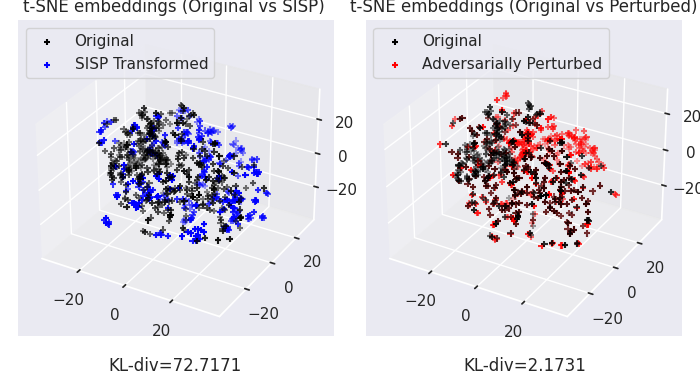
\includegraphics[width=\linewidth]{sdro/images/tsne_orig_both_pplx_5.png}
    \caption{
    Comparison of original sentences (black) with \textit{(left)} SISP-transformed sentences (blue) and \textit{(right)} \straightepsilon-bounded perturbations
    as a tSNE plot.
    }
    \label{fig:tsne}
\end{figure}
In order to quantify the diverse and larger semantic transformations compared to additive perturbations, 
we study the tSNE~\citep{van2008visualizing} embeddings of (i) original samples from NLVR$^2$ ($P$), (ii) their SISP-transformed versions ($P_{SISP}$), and (iii) their adversarially perturbed versions ($P_{adv}$).
Input sentences are encoded using the UNITER text encoder for (i) and (ii), and the adversarial perturbation mechanism~\citep{gan2020large} for (iii).
3D tSNE embeddings are visualized in Figure~\ref{fig:tsne}; SISP transformed sentences (blue) are farther away than the perturbed versions.
This shift is quantified by the KL-divergence~\citep{kullback1951information} between the distributions, with $D_{KL}(P_{SISP}||P) > D_{KL}(P_{adv}||P)$ implying that the diversity of SISP transformations is higher.


\subsection{Comparison of Model Calibration}
\begin{figure}
    \centering
    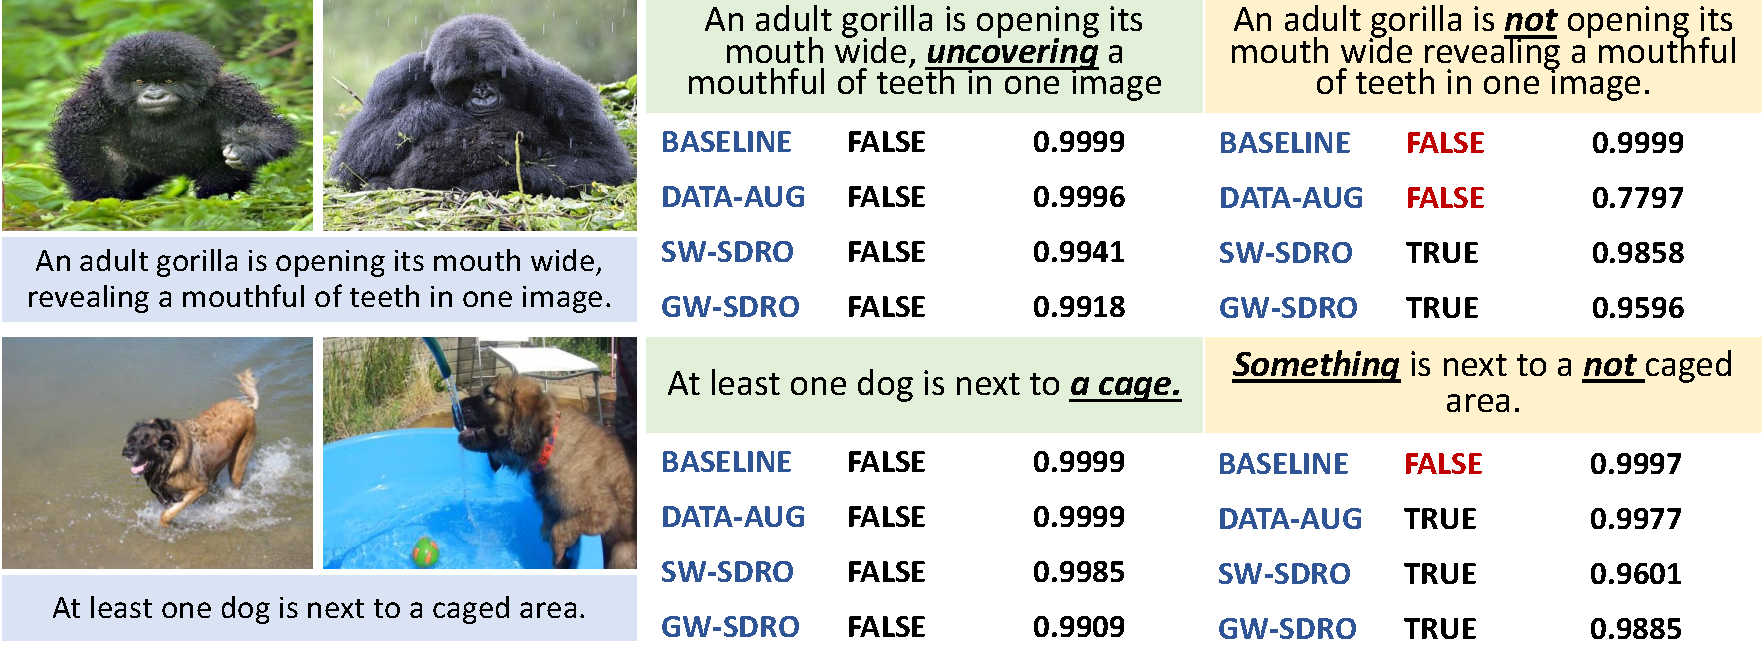
\includegraphics[width=\linewidth]{sdro/images/predictions_qualitative_2.pdf}
    \caption{
    Original test inputs for NLVR$^2$ with their respective SP (green) and SI (yellow) test samples and the prediction and confidence of models with VILLA backbone.
    Wrong predictions are highlighted in red.
    }
    \label{fig:qualitative}
\end{figure}
Figure~\ref{fig:qualitative} contains qualitative examples from NLVR$^2$ to compare output probabilities.
We observe that SDRO models have higher clean accuracy, but lower confidence in the predictions than baseline and \textit{data-aug} methods.
\paragraph{Reliability Diagrams.}
\begin{figure}
    \centering
    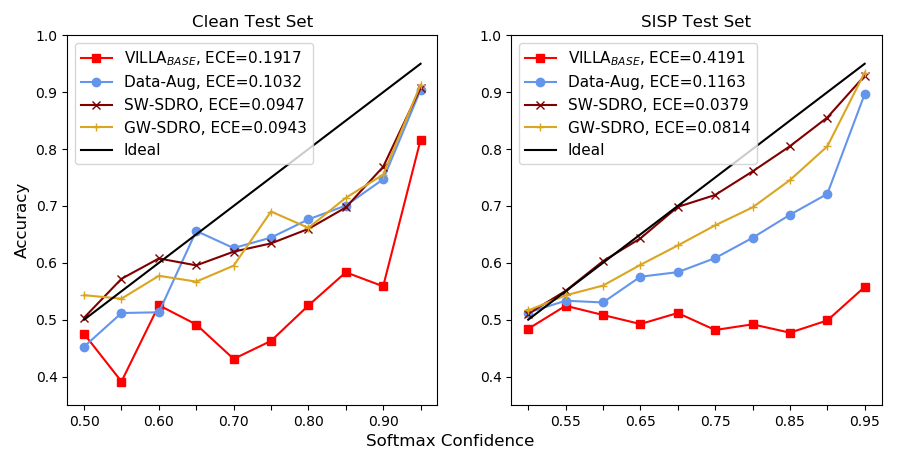
\includegraphics[width=\linewidth]{sdro/images/reliability.png}
    \caption{Comparison of reliability curves on the clean test set \textit{(left)} and SISP test set \textit{(right)}.}
    \label{fig:reliability}
\end{figure}
To validate this observation at scale, we use reliability diagrams to visualize model calibration~\citep{niculescu2005predicting}, and plot model accuracy as a function of confidence.
We use the softmax probability $\hat{p}$ of the predicted class as model confidence, split the range of probabilities into $M=20$ equal-sized bins, and calculate bin accuracy $acc(B_m)$ and bin confidence $conf(B_m)$~\citep{guo2017calibration}.
If $B_m$ is the set of all samples that fall in the $m^{th}$ bin,
\begin{align}
    acc(B_m) &\triangleq \frac{1}{|B_m|}\sum_{X_i\in B_m}\mathbbm{1}(\hat{y}_i = y_i), \\
    conf(B_m) &\triangleq \frac{1}{|B_m|}\sum_{X_i\in B_m} \hat{p}_i .
\end{align}
A model with perfect calibration should have a reliability diagram such that $$acc(B_m)=conf(B_m)$$.
We also report Expected Calibration Error~\citep{naeini2015obtaining} over all $n$ test samples:
\begin{equation}
    ECE=\sum_{m=1}^M\frac{|B_m|}{n}|acc(B_m){-}conf(B_m)|.
\end{equation}


Reliability diagrams and corresponding ECE values for the baseline VILLA trained with naive data augmentation and SDRO methods for NLVR$^2$ are shown in Figure~\ref{fig:reliability}.
On both the clean test set and SISP test set, SDRO models have the lowest ECE.
While the ECE for SDRO is marginally better than data augmentation for the clean test set, SDRO is much better calibrated for the SISP test set, with SW-SDRO closest to ideal calibration.

\subsection{Size of Training Dataset}
We evaluate models trained on small subsets of the original dataset, and compare their performance in Figure~\ref{fig:lowres}.
SDRO models are significantly better at all sizes of training datasets as shown by accuracy and AUC (area under the curve).
Notably, SDRO models trained with only $10\%$ ($\sim8.6K$) samples have performances similar to the baseline trained with $30\%$ samples;
SDRO models with $20\%$ data are better than the baseline model with $40\%$ data.
While models trained with naive augmentation saturate below SOTA, at ${\sim}80\%$ data size, SDRO models cross the existing SOTA of $78.39\%$.

\begin{figure}[t]
    \centering
    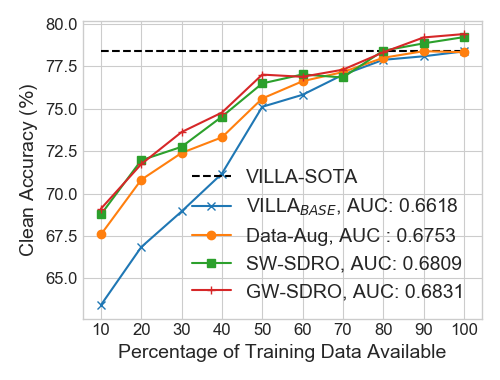
\includegraphics[width=0.49\linewidth]{sdro/images/lowResource_auc.png}
    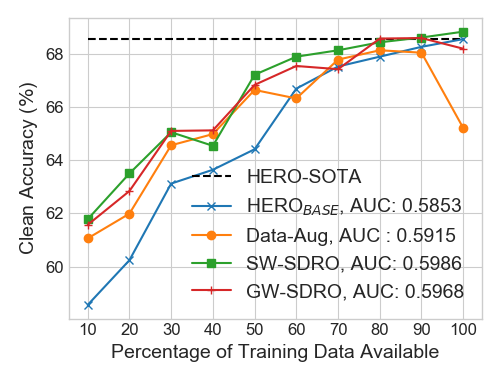
\includegraphics[width=0.49\linewidth]{sdro/images/violin_lowResource_auc.png}
    \caption{
    Effect of size of training data \textit{(left)} NLVR$^2$, \textit{(right)} VIOLIN.
    SDRO models are consistently better than baselines, even in low-data settings. 
    }
    \label{fig:lowres}
\end{figure}

\subsection{Ablation Studies}
\begin{figure}[t]
    \centering
    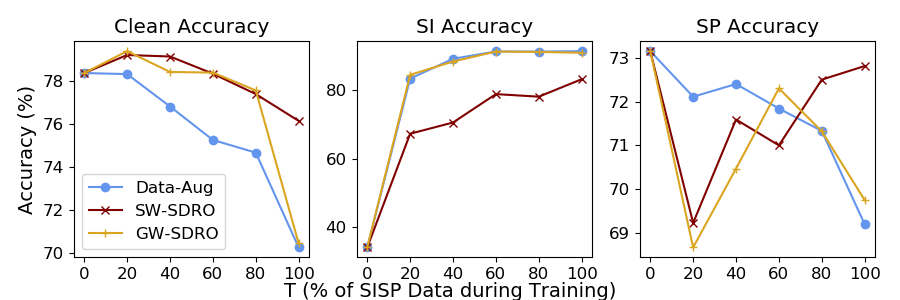
\includegraphics[width=\linewidth]{sdro/images/T_as_curve.png}
    \caption{
    Plots showing the effect of the percentage of augmented samples on Clean, SP, and SI accuracies on NLVR$^2$, when using data-augmentation, and SDRO.
    }
    \label{fig:NLVR2_ablation_T}
\end{figure}
\paragraph{Proportion of Augmented Samples.}
The final dataset has the same size as the original training set, but with T$\%$ transformed samples and $(100{-}T)\%$ original samples.
The effect of this hyperparameter $T$ is reported in Figure~\ref{fig:NLVR2_ablation_T} as a percentage improvement of accuracy w.r.t.\ VILLA$_{BASE}$.
An {optimal value of $T{=}20\%$ leads to improvements in clean accuracy}, but a larger proportion of augmented samples degrades performance.
Similarly, higher $T$ leads to higher robust accuracy, pointing to a \textul{trade-off between clean accuracy and robust accuracy at values of $T$ higher than the optimal}.
This conforms with similar findings from~\citet{tsipras2019robustness}.
While models trained with naive data-augmentation have better SISP accuracy than SDRO models as in Table~\ref{tab:results_nlvr2}, they do so by sacrificing clean accuracy, while SDRO models improve along both dimensions compared to the baselines.

\paragraph{Contributions of SI and SP independently:}
\begin{table}
    \centering
    \resizebox{\linewidth}{!}{
    \begin{tabular}{@{}l ccc c ccc c ccc@{}}
        \toprule
        \multirow{2}{*}{\textbf{Model}} & \multicolumn{3}{c}{SP only} & \hphantom & \multicolumn{3}{c}{SI Only} & \hphantom & \multicolumn{3}{c}{Both} \\ 
         \cmidrule{2-4} \cmidrule{6-8}  \cmidrule{10-12}
         & Clean & SP & SI && Clean & SP & SI && Clean & SP & SI \\
        \midrule
        Data-Aug & 76.07 & 74.89 & 35.77 && 69.51 & 53.68 & 94.89 && 78.34 & 72.11 & 84.44 \\
        SW-SDRO & 79.79 & 76.93 & 30.72 && 79.27 & 55.53 & 88.76 && 79.23 & 69.23 & 67.35 \\
        GW-SDRO & 79.46 & 75.72 & 33.04 && 79.13 & 54.31 & 93.25 && 79.41 & 68.67 & 84.54 \\
        \bottomrule
    \end{tabular}
    }
    \caption{Comparison of performance when only SP, only SI, or both types of transformations are performed.}
    \label{tab:analysis_si_sp_all}
\end{table} 
We analyze which of the two categories (semantics-inverting (SI) or semantics-preserving (SP)) is the most effective by performing SDRO with only SI transforms, or with only SP transforms, and when using both.
Table~\ref{tab:analysis_si_sp_all} shows that SDRO models trained only with SI suffer in terms of SP robustness and vice versa.
However, there is still an increase in clean accuracy in both cases.
This indicates that \textul{both SI and SP contribute towards improvements in robustness and clean accuracy.}


\paragraph{Transformations of only \texttt{True} statements:}
\begin{table}
    \centering
    % \footnotesize
    % \resizebox{\linewidth}{!}{
    \begin{tabular}{@{}l ccc c ccc@{}}
        \toprule
        \multirow{2}{*}{\textbf{Model}} & \multicolumn{3}{c}{SISP~(Pos)} & \hphantom & \multicolumn{3}{c}{SISP~(All)} \\ 
         \cmidrule{2-4} \cmidrule{6-8}
         & Clean & SP & SI && Clean & SP & SI \\
        \midrule
        Data-Aug & 78.23 & 68.02 & 57.48 && 78.34 & 72.11 & 84.44 \\
        SW-SDRO  & 78.81 & 62.06 & 66.07 && 79.23 & 69.23 & 67.35 \\
        GW-SDRO  & 79.10 & 63.47 & 62.29 && 79.41 & 68.67 & 84.54\\
        \bottomrule
    \end{tabular}
    % }
    \caption{Comparison of performance if only positive samples 
    % or both positive or negative samples 
    % i.e.\ samples with \texttt{True} labels 
    are used as inputs for SISP transformations
    % ,  transformations over both positive and negative samples.
    }
    \label{tab:analysis_pos_all}
\end{table} 
Transforming \textit{False} (negative) statements can lead to ambiguous and subjective meanings~\citep{russell1905denoting}.
We investigate if transforming only \textit{True} (positive) statements is better than transforming both \textit{True} and \textit{False} statements.
Table~\ref{tab:analysis_pos_all} shows that SISP transformations of both types of statements lead to higher clean accuracy and robustness.

\subsection{Robustness to Text-Attacks}

% \begin{table}[t]
%     \centering
%     \resizebox{\linewidth}{!}{
%     \begin{tabular}{@{}cl ccccccc@{}}
%         \toprule
%         % \multirow{2}{*}{\textbf{Model}} & \multicolumn{7}{c}{\textbf{Text Attack Categories}} \\
%         % \textbf{Dataset}
%         & \textbf{Model} & \textbf{CR} & \textbf{CS} & \textbf{CL} & \textbf{EDA} & \textbf{Emb} & \textbf{WN} & \textbf{Avg.}\\
%         \midrule
%         % LX          & 74.38 & 72.45 & 70.72 & 67.73 & 71.26 & 72.12 & 71.44 \\
%         % LX + SDRO   & 70.18 & 67.96 & 65.94 & 64.29 & 69.05 & 66.49 & 67.32 \\
%         % \midrule  
%         % UN          & 75.35 & 75.44 & 73.99 & 69.02 & 74.96 & 73.45 & 73.70 \\
%         % UN + SDRO   & 75.71 & 75.35 & 71.14 & 68.84 & \underline{76.44} & 75.24 & 73.79 \\
%         % \midrule 
%         \multirow{2}{*}{NLVR$^2$} 
%         & VILLA          & 77.45 & 74.38 & \underline{74.42} & 69.62 & 75.45 & 75.87 & 74.52 \\
%         & \quad + SDRO   & \underline{78.51} & \underline{77.20} & 72.06 & \underline{71.08} & 75.77 & \underline{76.41} & \textbf{75.17}\\
%         \midrule
%         \multirow{2}{*}{VIOLIN} 
%         & HERO          & 66.08  & 63.00 & 68.58 & 60.89 & 63.81 & 63.38 & 64.29 \\
%         & \quad + SDRO   & 68.70 & 64.95 & 68.96 & 61.32 & 65.54 & 64.61 & 65.68 \\
%         \midrule
%         \multirow{2}{*}{\shortstack{VQA \\Yes/No}} 
%         & VILLA          & 80.49 & 75.74 & 84.87 & 74.64 & 78.63 & 76.39 & 78.45 \\
%         & \quad + SDRO   & 85.99 & 84.52 & 84.10 & 87.02 & 84.25 & 84.03 & 84.99 \\
%         \bottomrule
%     \end{tabular}
%     }
%     \caption{Performance on ``text-attack''~\cite{morris2020textattack} versions of the NLVR$^2$, VIOLIN, and VQA-Yes/No test sets. CR: CLARE; CS: CharSwap, CL: Check-List, EDA: Easy Data Augmentation, Emb: Embedding-based, WN: WordNet-based.}
%     \label{tab:text_attack}
% \end{table}

\begin{table}
    \centering
    % \small
    % \resizebox{\linewidth}{!}{
    \begin{tabular}{@{}cl ccccccc@{}}
        \toprule
        & \textbf{Model} & \textbf{CR} & \textbf{CS} & \textbf{CL} & \textbf{EDA} & \textbf{Emb} & \textbf{WN} & \textbf{Avg.}\\
        \midrule
        \multirow{2}{*}{NLVR$^2$} 
        & VILLA          & 77.5 & 74.4 & \underline{74.4} & 69.6 & 75.5 & 75.9 & 74.5 \\
        & \quad + SDRO   & \underline{78.5} & \underline{77.2} & 72.1 & \underline{71.1} & 75.8 & \underline{76.4} & \textbf{75.2}\\
        \midrule
        \multirow{2}{*}{VIOLIN} 
        & HERO          & 66.1  & 63.0 & 68.6 & 60.9 & 63.8 & 63.4 & 64.3 \\
        & \quad + SDRO   & 68.7 & 65.0 & 69.0 & 61.3 & 65.5 & 64.6 & 65.7 \\
        \midrule
        \multirow{2}{*}{\shortstack{VQA \\Yes/No}} 
        & VILLA          & 80.5 & 75.7 & 84.9 & 74.6 & 78.6 & 76.4 & 78.5 \\
        & \quad + SDRO   & 86.0 & 84.5 & 84.1 & 87.0 & 84.3 & 84.0 & 85.00 \\
        \bottomrule
    \end{tabular}
    % }
    \caption{Performance on ``text-attack'' of NLI test set.
    % ~\cite{morris2020textattack} versions of the NLVR$^2$, VIOLIN, and VQA-Yes/No test sets. 
    % CR: CLARE, CS: CharSwap, CL: Check-List, EDA: Easy Data Aug, Emb: Embedding-based, WN: WordNet-based.
    }
    \label{tab:text_attack}
\end{table}
We utilize automated adversarial attack recipes~\citep{morris2020textattack}:
CLARE (CR)~\citep{li2021contextualized}, character-swap (CS)~\citep{pruthi2019combating}, Checklist (CL)~\citep{ribeiro2020beyond}, EDA~\citep{wei2019eda}, counter-fitted embeddings (Emb)~\citep{alzantot2018generating}, and WordNet-based swap~\citep{ren2019generating}.
Table~\ref{tab:text_attack} shows results using the best backbone and our SDRO model.
On NLVR$^2$, VILLA+SDRO is better than VILLA for 4 out of 6 attack categories, and $0.65\%$ on average.
On VIOLIN, HERO+SDRO outperforms the baseline on all attack categories, leading to an average gain of $1.39\%$.
On VQA-Yes/No, VILLA+SDRO outperforms the baseline on all attack categories, and $6.54\%$ on average.


%-------------------------------------------------------------------------
% %%%%%%%%% RELATED WORK
% \section{Related Work}

% \textbf{Adversarial Training} (AT)
% has been studied under a game-theoretic~\citep{dalvi2004adversarial} and
% min-max setup~\citep{madry2018towards}.
% \citet{volpi2018generalizing} use AT to adversarially augment image classification datasets and show improved domain generalization for digit classification.
% \citet{wong2020learning,gokhale2020attribute} modify AT for real-world adversaries beyond norm-bounded perturbations.
% AT has been used for text classification with LSTMs~\citep{miyato2016adversarial} and for pretraining transformer-based models by adding label-preserving adversarial perturbations to embeddings of word tokens~\citep{zhu2020freelb,jiang2020smart,gan2020large}
% Contrastive examples have been explored, collected from humans~\citep{agrawal2018don}, negative mining~\citep{shi2018learning}, or synthetic generation~\citep{agarwal2020towards,chen2020counterfactual,gokhale2020mutant,teney2020learning}.

% \textbf{Robustness in V\&L}
% has been explored for VQA, such as performance under prior probability shift~\citep{agrawal2018don} and domain adaptation~\citep{chao2018cross,xu2019open}, along with robustness for implied questions~\citep{ribeiro2019red} and novel compositions~\citep{johnson2017clevr,agrawal2017c}, and robustness to logical connectives (including negation)~\citet{gokhale2020vqa}.
% \citet{teney2020learning} have shown that many V\&L, image classification, and sentiment analysis models are sensitive to image editing.
% There has been a recent effort of model-in-the-loop dataset collection to guide humans to create harder VQA samples~\citep{li2021adversarial,sheng2021human}.

% \textbf{Robustness in NLP:}
% Generation of SP adversarial examples 
% \citep{jia2017adversarial,ribeiro2018semantically,iyyer2018adversarial,alzantot2018generating}, and approaches to defend against word substitution~\citep{jia2019certified} have been explored.
% Evaluation datasets have also been proposed for textual entailment that are manually crafted~\citep{gardner2020evaluating} or template-based~\citep{mccoy2019right,glockner2018breaking,naik2018stress}.
% Our method uses automated linguistically-informed SI and SP transforms for both training and inference.
%-------------------------------------------------------------------------
%%%%%%%%% DISCUSSION 
\section{Discussion}
\paragraph{On Ensembling Coefficients.}
While designing our ensembling approach, we used $\alpha=0.5$, i.e., equal contribution from the original output and the average of all outputs for transformed samples.
This choice is generic and does not rely on dataset- or model-specific characteristics of SISP accuracy.
While treating $\alpha$ as a hyperparameter and tuning it on validation datasets could lead to further gains, our intuitive choice of $\alpha{=}0.5$ is effective by itself.

\paragraph{On SI Samples.}
Tables~\ref{tab:results_nlvr2},~\ref{tab:results_violin},~\ref{tab:results_vqayesno} show that existing models perform well on SP transforms, implying that equivalent semantics are captured in transformer-based models.
However, these models fail on SI samples, and thus the average SISP accuracy is close to random $(50\%)$. 
When images are perturbed with noise, blur, weather, or digital artifacts~\citep{hendrycks2018benchmarking}, they retain semantics -- an image of a ``cat'' remains a cat after perturbation.
However, for text inputs, minimal changes to the sample, such as a single word changing from ``sitting'' to ``standing'' or ``not sitting'', inflict large changes in meaning.
We hope that future work on design of V\&L evaluation criterion along the SI axis, could benefit from our findings.
While we generated SI and SP text for VLI tasks, the idea could be extended to design SISP transformations for images, by operating at object-level instead of pixel-level

\paragraph{On combination of AT and SDRO.}
We show that combining AT with SDRO can improve VLI performance and incorporate domain knowledge into the training process, such as semantic knowledge that often exists in natural language or linguistic rules.
This is explicitly observed with VILLA, which is pre-trained and fine-tuned using standard adversarial training~\citep{gan2020large}.
When fine-tuned with SDRO, VILLA+SDRO further improves compared to UNITER+SDRO.
The combination of standard adversarial training, (which accounts for local adversaries inside a $\epsilon$ norm-ball) and SDRO, (which accounts for linguistic adversaries and contrastive examples, typically outside the norm-ball as shown in Figure~\ref{fig:vector_vs_linguistic}) could lead to improved generalization in many other V\&L tasks.

\paragraph{On differentiability.}
Linguistic transforms are not differentiable and prohibit gradient-based solutions to the inner maximization in SDRO.
Nevertheless, we show that explicitly choosing the $argmax$ over a pre-defined set of transformations does indeed lead to model-agnostic improvements for multiple V\&L tasks.
This is a first step towards incorporating domain knowledge into adversarial training. 
More sophisticated methods may emerge in the future to address non-differentiability by leveraging proximal point or trust-region methods~\citep{eckstein1993nonlinear,conn2000trust} or Interval Bound Propagation~\citep{dvijotham2018dual,jia2019certified}.

 
%-------------------------------------------------------------------------


\begin{abstract}
Captioning is a crucial and challenging task for video understanding.  
In videos that involve active agents such as humans, the agent's actions can bring about myriad changes in the scene. 
Observable changes such as movements, manipulations, and transformations of the objects in the scene, are reflected in conventional video captioning.
Unlike images, actions in videos are also inherently linked to social aspects such as intentions (why the action is taking place), effects (what changes due to the action), and attributes that describe the agent. 
Thus for video understanding, such as when captioning videos or when answering questions about videos, one must have an understanding of these commonsense aspects.
We present the first work on generating \textit{commonsense} captions directly from videos, to describe latent aspects such as intentions, effects, and attributes.
We present a new dataset ``Video-to-Commonsense (V2C)" that contains $\sim9k$ videos of human agents performing various actions, annotated with 3 types of commonsense descriptions.
Additionally we explore the use of open-ended video-based commonsense question answering (V2C-QA) as a way to enrich our captions.
Both the generation task and the QA task can be used to enrich video captions.
\end{abstract}

%%%%%%%%%%%%%%%%%%%%%%%%%%%%%%%%%%%%%%%%%%%%%%%%%%%%%%%%%%%%%%%%
% INTRODUCTION
%%%%%%%%%%%%%%%%%%%%%%%%%%%%%%%%%%%%%%%%%%%%%%%%%%%%%%%%%%%%%%%%
\section{Introduction}
\begin{figure*}
    \centering
    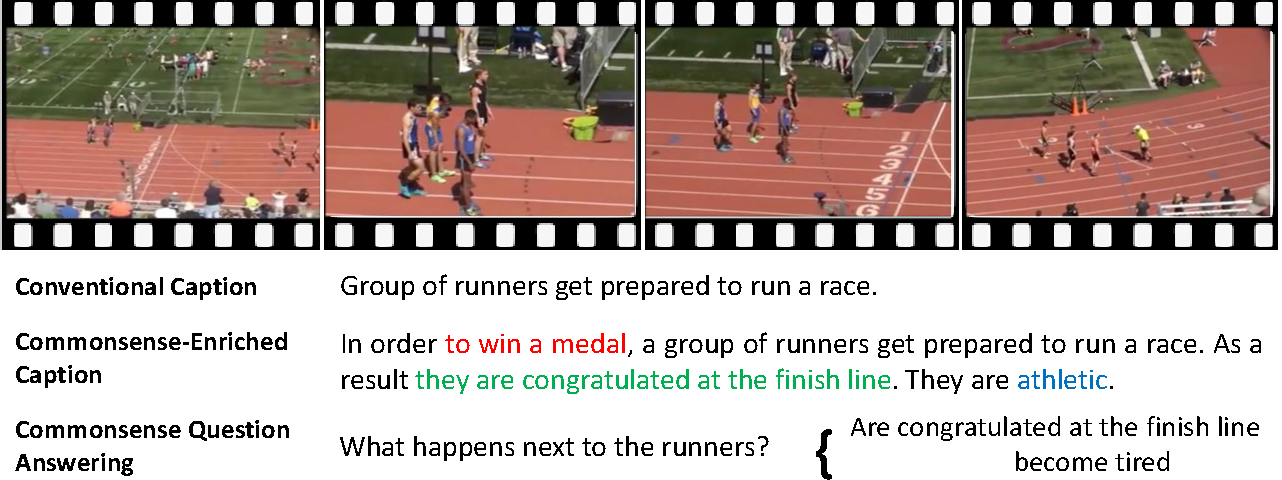
\includegraphics[width=0.9\linewidth]{v2c/fig/teaser_single.pdf}
    \caption{Comparison of conventional video captioning with our commonsense-enriched captioning. Our captions describe intention behind the action ({\color{red}red}), attribute of the agent ({\color{blue}blue}), and effect of the action on the agent ({\color{green}green}).}
    \label{fig:pipeline}
\end{figure*}

When humans watch videos they can typically understand and reason about various aspects of the scene beyond the visible objects and actions.
This involves understanding that some objects are \textit{active agents} that not only perform actions and manipulate objects, but are motivated by intentions, have pre-conditions, and that their actions have an effect on the world and their own mental states.
For instance, in analyzing the video clip in Figure~\ref{fig:pipeline}, humans employ various capabilities such as perception, reasoning, inference, and speculation, to come up with a description for the observable sequence of events, but also reason about latent aspects such as the intention of the group of runners \textit{``to win the medal"}, the effect of being \textit{``congratulated at the finish line"}, and the attribute \textit{``athletic"}.

The above example also illustrates that recognition of objects, actions, and events is often not enough; understanding causal relationships, social interactions, and commonsense aspects behind them provides context and a more semantic interpretation of the video~\cite{gupta2009understanding}.
A model that can provide such detailed interpretations facilitates answering inferential questions, such as \textit{``Will the player get angry later?"}.
However, existing visual understanding systems are unable to perform such tasks that require speculative reasoning.
A critical missing element in complex video understanding is the capability of performing commonsense inference, especially a generative model.
Existing efforts seek to find textual explanations or intentions of human activities as a classification task~\cite{vondrick2016predicting} or a vision-to-text alignment problem~\cite{zhu2015aligning}.

In this paper we propose the \textbf{V}ideo to \textbf{C}ommonsense (V2C) framework to generate visually grounded commonsense descriptions about the underlying event in the video, enriching the factual description provided by a caption.
Under this framework a system is expected to generate captions as well as three types of commonsense descriptions (intention, effect, attribute) directly from an input video.
The V2C model can also be used as a building block for downstream tasks such as video question answering for questions requiring commonsense.
Inspired by~\citep{bosselut2019comet}, our model -- the ``V2C-Transformer" utilizes: (1) a video encoder to extract global representations of the video, (2) a transformer decoder that generates captions and commonsense descriptions, and (3) a cross-modal self-attention module that exploits joint visual-textual embeddings.

We curate the V2C dataset for training and benchmarking models on this task.
We adopt the MSR-VTT video description dataset~\citep{xu2016msr} as a source of videos and captions.
We first utilize the A\textsc{tomic} machine commonsense dataset~\cite{sap2018atomic} to get a list of candidate commonsense texts (intentions, effects, and attributes), and rank these using a BERT-based~\cite{devlin2018bert} model.
Since these candidates are retrieved without using the video and may not be accurate, we instruct humans to watch the videos and select, remove, or rewrite the texts retrieved from A\textsc{tomic}.
The text retrieved by A\textsc{tomic} helps our human annotators to understand the format of desired annotations, and also gives them a list of suggestions.
The human component in our annotation procedure makes our data visually grounded and relevant, linguistically diverse, and natural.

We additionally explore the use of our V2C-Transformer architecture for a open-ended video question answering task, where the questions are about commonsense aspects from the video.
For this, we create a QA addendum of the V2C dataset called V2C-QA.
By asking questions about the latent aspects in the video, our models are able to enrich caption generation with three specific types of commonsense knowledge.

Our contributions are summarized below:
\begin{enumerate}[noitemsep,nosep]
    \item We formulate the ``V2C" task for enriching video captioning by generating descriptions of commonsense aspects.
    \item We curate a video dataset annotated with captions and commonsense descriptions.
    \item We present our V2C-Transformer architecture that generates relevant commonsense descriptions, and serves as a strong baseline.
    \item We pose V2C as a video question answering task and show that it can assist commonsense caption generation.
\end{enumerate}


%%%%%%%%%%%%%%%%%%%%%%%%%%%%%%%%%%%%%%%%%%%%%%%%%%%%%%%%%%%%%%%%
% V2C
%%%%%%%%%%%%%%%%%%%%%%%%%%%%%%%%%%%%%%%%%%%%%%%%%%%%%%%%%%%%%%%%
\section{Video to Commonsense (V2C)}
\paragraph{Problem Formulation:} 
Consider a video $\mathit{V}$ consisting of $N_v$ frames described by sentence $\mathit{S}$. 
Our Video-to-Commonsense (V2C) framework can be used for generating commonsense descriptions $\mathit{C}$ under two settings.
In the first setting (\textbf{V2C-Completion}), we use ground-truth captions to guide commonsense-enriched caption generation.
This task can be viewed as providing supplementary explanations to the caption.
In the second setting (\textbf{V2C-Generation}), we first learn to generate captions from videos, $\mathbf{g}(\mathit{V})$, and then use them to generate commonsense descriptions.
\begin{align}
    \small
    \begin{split}
        \textbf{V2C-Completion}  \quad \mathit{C} &= \mathbf{f}(\mathit{V}, \mathit{S}).\\
        \small
        \textbf{V2C-Generation}  \quad \mathit{C} &= \mathbf{f}(\mathit{V}, \mathbf{g}(\mathit{V})).
    \end{split}
\end{align}

    \subsection{V2C-Transformer}
    \begin{figure*}[t]
        \centering
        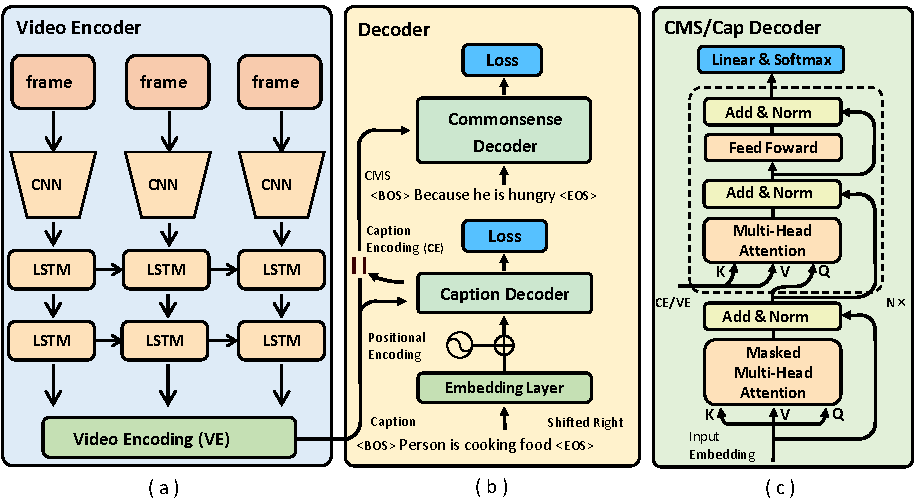
\includegraphics[width=.9\textwidth]{./v2c/fig/architecture.pdf}
        \caption{
        The V2C-Transformer model architecture contains:
        \textbf{(a)} Video Encoder designed to take video frames as input and encode them into frame-wise representations, 
        \textbf{(b)} Decoder module consisting of a Caption Decoder and a Commonsense Decoder, and
        \textbf{(c)} Transformer Decoder module containing a stack of $N$ consecutive transformer blocks (shown inside the dashed area).
        }
        \label{fig:architecture}
    \end{figure*}
    
    The proposed Video2Commonsense Transformer is a cross-modal model that generates captions and commonsense-enriched descriptions from videos. 
    Our approach (Figure \ref{fig:architecture}) adopts the ``encoder-decoder'' design: a video encoder that extracts global representations of the input video, and a transformer decoder that produces relevant commonsense knowledge along with captions.
    
    \paragraph{Video Encoder:}
    We obtain per-frame ResNet-152~\cite{he2016deep} features for video $\mathit{V}$ and process them using an LSTM model~\cite{sundermeyer2012lstm}, a standard architecture for modeling long temporal sequences, and use the last hidden states of the LSTM as the video representations.
    We concatenate all previous hidden states from each LSTM module as a final global video encoding $\mathbf{v}$, to provide the model with explicit context using the temporal attention mechanism.
    
    \paragraph{Decoder:}
    The video encoding is used as input to two decoder networks that use a transformer language model~\cite{radford2018improving} to generate a caption and commonsense description, using an inference mechanism similar to~\citet{bosselut2019comet}.
    Our model is a two-stage process that first predicts the current events directly from videos, and then produces the corresponding commonsense captions. 
    During training, the caption decoder $\mathbf{D}_{\textsc{CAP}}$ takes the video encoding ($\mathbf{v}$) and ground truth caption ($\mathbf{s}$) as input to generate caption encoding ($\mathbf{\hat{s}}$), while the commonsense decoder $\mathbf{D}_{\textsc{CMS}}$ uses the concatenation of video and caption encoding to obtain the commonsense description ($\mathbf{c}$), as shown in Figure~\ref{fig:pipeline} (b).
    This arrangement enables the attention module in commonsense decoder to attend to both the video and caption context. 
    \begin{equation}
    \small
        \mathbf{\hat{s}} = \mathbf{D}_{\textsc{CAP}}(\mathbf{v},  \mathbf{s}),  \quad 
        \mathbf{c} = \mathbf{D}_{\textsc{CMS}}(\mathbf{v},  \mathbf{\hat{s}}).
    \end{equation}

    
    \noindent\textbf{Transformer Decoder}
    is composed of a stack of transformer blocks (dashed area in (c) Figure~\ref{fig:architecture}), whose main component is a self-attention architecture.
    It takes as input the summation of word embedding and the positional encoding offset by 1 position through masked multi-head attention, which prevents the future words been seen. 
    In our model, we deploy two stacked decoder architectures for both caption decoding and commonsense knowledge decoding.
    The Transformer Block consists of consecutive linear transformation: a multi-head attention module (denoted as $\mathcal{H}_{\textsc{M-Att}}$), a two-layer feed forward network ($\mathcal{H}_{\textsc{FFN}}$), a layer normalization operation, and a residual connection.
        
    \paragraph{Multi-head Attention module} 
    To enable our transformer decoder to generate commonsense descriptions by using both the visual and textual content, we modify the multi-head attention module (which acts as the basic unit in recent transformer based language generation models~\cite{radford2018improving,radford2019language}) as a cross-modal module.
    $\mathcal{H}_{\textsc{M-Att}}$ takes the input of the embedding of key (K), value (V) and query (Q).
    The key and value in transformer block are the video encoding (caption decoder) or concatenation of video/caption encoding (commonsense decoder), while the query is the output from the previous transformer block. 
    In the masked multi-head attention module, K, V and Q are the identical vectors of input embedding.
    For a self-attention block with $h$ heads,
        \begin{equation}
        \small
            \mathcal{H}_{\textsc{M-Att}}(\textsc{K}, \textsc{V}, \textsc{Q}) = \mathcal{H}_{\textsc{FFN}}([x_1,\dots, x_h]),
        \end{equation}
        where $x_i$ is computed by scaled dot-product attention operation, for head-index $i$, key-dimension $d_k$n, and transformation parameters $\textsc{w}_i$. 
        \begin{equation}
        \small
        \begin{split}
            \textbf{for } \mathbf{D}_{\textsc{CAP}}, &\quad {x_i} = \textsc{Softmax}(\frac{\textsc{w}^\textsc{q}_i \textsc{Q}\cdot \textsc{w}^\textsc{k}_i \textsc{K}^\prime}{\sqrt{d_k}})\textsc{w}^\textsc{v}_i \textsc{V}, \\
            \textbf{for } \mathbf{D}_{\textsc{CMS}}, &\quad {x_i} = \textsc{Softmax}(\frac{\textsc{w}^\textsc{q}_i [\mathbf{v},  \mathbf{s}]\cdot \textsc{w}^\textsc{k}_i [\mathbf{v},  \mathbf{s}]^\prime}{\sqrt{d_k}})\textsc{w}^\textsc{v}_i \textsc{V}.
        \end{split}
        \nonumber
        \end{equation}
            
        



%%%%%%%%%%%%%%%%%%%%%%%%%%%%%%%%%%%%%%%%%%%%%%%%%%%%%%%%%%%%%%%%%%%%%%%%%%%%%%%
% DATASET
%%%%%%%%%%%%%%%%%%%%%%%%%%%%%%%%%%%%%%%%%%%%%%%%%%%%%%%%%%%%%%%%%%%%%%%%%%%%%%%

\section{The V2C Dataset}
\begin{figure}[t]
    \centering
    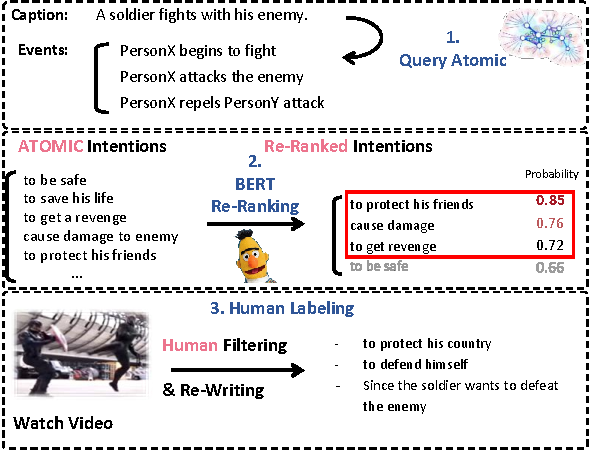
\includegraphics[width=\linewidth]{v2c/fig/v2cdataset.pdf}
    \caption{The overall three-step pipeline (retrieval from ATOMIC, BERT re-ranking, and human labeling) to construct our V2C dataset.}
    \label{fig:v2cdataset}
\end{figure}

For the V2C task we need video clips annotated with commonsense descriptions about the agents in the video, as shown in Figure~\ref{fig:pipeline}.
While there are video captioning datasets such as  MSR-VTT~\cite{xu2016msr}, the captions in these datasets describe only the observable objects in the image, but do not describe latent and commonsense aspects.
We are the first to curate such a dataset with annotations describing the intention of agent to perform an action, the effect of the action and the attribute of the agent given the action.

\paragraph{M{SR-VTT}} contains around 10k videos each 10 to 30 seconds long, belonging to 20 categories covering a variety of topics such as sports, music, news, and home videos.
Each video is accompanied by 20 human-annotated textual descriptions on average.
For training and benchmarking the novel V2C task,  we further complement MSR-VTT with event-level commonsense annotations, i.e. event descriptions with intentions, effects and attributes. 
We remove captions and videos that do not have clear human activities.
This is because having such videos leads to an imbalance in the number of captions for each video, thus making it inappropriate to just evaluate caption generation using BLEU scores.

\paragraph{A\textsc{TOMIC}}\cite{sap2018atomic} is an atlas of everyday commonsense knowledge and contains 880k triplets about causes and effects of human activities, organized as \textit{if-then} relations, annotated by crowd-sourced workers.
This data can be categorized based on causal relations, thereby giving us the categories ``cause", ``effect" and ``attribute", e.g., ``\textit{if} X wants to relax, \textit{then} he will play video game."
    
    \subsection{Querying from ATOMIC and Re-ranking}
    \begin{table}[t]
    \begin{center}
      \resizebox{\linewidth}{!}{
        \begin{tabular}{@{}p{0.7cm}c>{\RaggedRight}p{4.3cm}>{\RaggedRight}p{3.2cm}@{}}
        \toprule
        \textbf{Type} & \phantom{a} & \textbf{Video Caption} & \textbf{Commonsense} \\ 
        \toprule
        \multirow{2}{*}{Intention} 
        &  & Two guys are wrestling & to beat the opponent \\
        &  & {A man and woman are singing}  & to express themselves musically \\
         \midrule
         \multirow{2}{*}{Attribute} 
         & & A guy is singing in a crowd  & outgoing\\
         & & Group of riders race on motorcycles. & adventurous  \\
         \midrule
         \multirow{2}{*}{Effect}
         & & A person is making a paper airplane & gets excited to fly it \\
         & & A man and a woman are talking to each other & share ideas and opinions \\
        \bottomrule
        \end{tabular}
        }
    \end{center}
    \caption{Examples of commonsense annotations (intentions, attributes and effects) retrieved from A\textsc{tomic} for captions in MSR-VTT.}
    \label{tab:atomic_generations}
\end{table}
    
    Since inferential knowledge in A\textsc{tomic} only covers human activities, we first retain only those captions in {M{sr-vtt}} that describe human activities.
    We then select three queries from A\textsc{tomic} most similar to the caption, and extract the commonsense descriptions corresponding to these queries.
    In order to select a more reasonable subset of commonsense descriptions, we first train a ranking model.
    We use the BERT~\cite{devlin2018bert} architecture for the ranking model, trained on the ATOMIC dataset for a binary classification task, to predict the relevance of a candidate commonsense description with respect to the event.
    We select the top three relevant intentions, effects, and attributes for each caption.
    This allows us to obtain a preliminary set of 9 commonsense annotations per video directly from the A\textsc{tomic} dataset, relevant to the caption, albeit with noise and annotations that are not relevant to the video.

\begin{table*}[t]
    
    \begin{center}
    \resizebox{\linewidth}{!}{
    \begin{tabular}{@{}p{1.7cm}c  p{5.7cm} c c cccc c c }
        \toprule
        \textbf{Relation} & \hphantom &
        \textbf{Model}  &
        \textbf{\# Param (M)}  &
        \textbf{CIDER} &             
        % \textbf{PPL $\downarrow$} &             
        \textbf{BLEU-1} &
        \textbf{BLEU-2} &
        \textbf{BLEU-3} &
        \textbf{BLEU-4} &
        \textbf{METEOR} &
        \textbf{ROUGE-L} \\
        \toprule
        % \multirow{4}{*}{{\normalsize {\textbf{Attribute}}}} 
        % && S2VT~\cite{venugopalan2015sequence}  & - & - & 35.9 & - & - & - & - & - \\
        % && Attention-Enc-Dec~\cite{gao2017video}  & - & - & 38.3 & - & - & - & - & -  \\
        % && Dense Captioner~\cite{zhou2018end}  & - & - & 46.0 & - & - & - & - & -\\
        % && Video CMS Transformer & - & - & 47.3 & - & - & - & - & -\\
        % \hline
        % \multirow{4}{*}{{\normalsize {\textbf{Effect}}}} 
        % && S2VT~\cite{venugopalan2015sequence} & 28.3 & 23.6 & 24.9 & 18.6 & 16.2 & 14.3 & 15.4 & 22.1  \\
        % && Attention-Enc-Dec~\cite{gao2017video} & 29.5 & 22.0 & 26.5 & 19.4 & 18.8 & 15.1 & 17.5 & 23.9   \\
        % && Dense Captioner~\cite{zhou2018end} & 36.9 & 16.0 & 33.7 & 24.8 & 21.0 & 20.2 & 20.0 & 29.9  \\
        % && Video CMS Transformer & 37.3 & 15.6 & 34.8 & 25.9 & 22.5 & 20.4 & 20.8 & 30.6  \\
        % \hline
        % \multirow{4}{*}{{\normalsize {\textbf{Intention}}}} 
        % && S2VT~\cite{venugopalan2015sequence} & 51.8 & 17.8 & 48.4 & 39.9 & 34.3 & 26.4 & 23.3 & 44.3\\
        % && Attention-Enc-Dec~\cite{gao2017video} & 52.1 & 16.0 & 51.1 & 42.6 & 35.5 & 28.2 & 24.3 & 48.0\\
        % && Dense Captioner~\cite{zhou2018end} & 60.3 & 12.0 & 59.3 & 47.0 & 37.3 & 31.5 & 28.0 & 53.1 \\
        % && Video CMS Transformer & 62.0 & 11.7 & 60.8 & 48.4 & 39.1 & 34.1 & 28.5 & 54.6  \\
        
        % Results updating due to new version V2C dataset, baselines are re-implemented and now we have 5-GT so numbers are all different.
        \multirow{4}{*}{{\normalsize {\textbf{Attribute}}}} 
        && RNN Encoder + Decoder & 66.0 & - & 21.7 & - & - & - & - & -  \\
        && Attention + Video2Text  & 52.5  & - & 36.5 & - & - & - & - & - \\
        && Transformer Encoder + Decoder  & 69.7 & - & 40.7 & - & - & - & - & -\\
        && Video CMS Transformer & 69.2 & -  & 47.3 & - & - & - & - & -\\
        \hline
        \multirow{4}{*}{{\normalsize {\textbf{Effect}}}} 
        && RNN Encoder + Decoder  & 66.0  & 12.2 & 21.2 & 11.5 & 8.6 & 7.5 & 10.2 & 16.7  \\
        && Attention + Video2Text & 52.5  & 18.5 & 27.7 & 16.9 & 13.3 & 11.5 & 16.0 & 23.9  \\
        && Transformer Encoder + Decoder & 69.7  & 37.7 & 35.3 & 26.6 & 23.2 & 21.0 & 21.4 & 31.1  \\
        && Video CMS Transformer & 69.2 & 40.8 & 36.5 & 28.1 & 24.6 & 22.4 & 22.2 & 32.3  \\
        \hline
        \multirow{4}{*}{{\normalsize {\textbf{Intention}}}} 
        && RNN Encoder + Decoder & 66.0 & 19.3 & 41.7 & 26.4 & 16.6 & 11.7 & 16.5 & 36.4 \\
        && Attention + Video2Text  & 52.5 & 23.2 & 54.3 & 40.0 & 27.4 & 24.7 & 19.4 & 45.6 \\
        &&  Transformer Encoder + Decode & 69.7 & 57.4 & 58.3 & 45.7 & 36.3 & 31.1 & 27.4 & 53.2 \\
        && Video CMS Transformer & 69.2 & 62.0 & 60.8 & 48.4 & 39.1 & 34.1 & 28.5 & 54.6  \\
        \hline
    \end{tabular}
    }
    \end{center}
    \caption{ Evaluation of V2C completion task using CIDER, BLEU, Rouge, and Meteor metrics. We use only BLEU-1 to evaluate the attribute generation  since the average length of the ground truth is just less than 2.}

    \label{tab:automaticevaluation}
\end{table*}
    \subsection{Detailed Human Annotation}
    Since we do not use the video to retrieve commonsense descriptions from ATOMIC, we employ human workers to annotate our dataset.
    We recruit two sets of human workers to watch the video, read the caption and select/annotate the relevant commonsense descriptions for each video.
    The first set is Amazon Mechanical Turkers (AMT) who select relevant descriptions.
    The second set is skilled human annotators, screened from a set of university students proficient in English, who are asked to provide annotations in their own words, and remove or edit irrelevant annotations that were provided by ATOMIC and AMT workers.
    This makes our annotations not only grounded in the video, but also more descriptive, linguistically diverse, and of higher quality (see Figure~\ref{fig:v2cdataset}).
    The descriptions from ATOMIC, although not relevant to the video in some cases, give our workers an idea about the format of annotations desired.
    The skilled humans reported that $95\%$ of the captions were relevant, and $65\%$ of the ATOMIC descriptions were useful in understanding the annotation task. Through this procedure, we obtain 6819 videos for training and 2906 videos for testing, a total of 121,651 captions ($\sim$12 captions/video), each caption accompanied with 5 commonsense knowledge annotations (V2C-Raw set). In experiment, we use video captioning technique to conduct the V2C completion task on V2C-Raw set.
    In addition, we instruct human annotators to select and rewrite one raw phrase into complete sentences that complement the captions.
    In total we have 3 complete sentences per video for intention/effect/attribute respectively, and this yields a subset that allows our model to generate complete story-like sentences (V2C-Clean Set).
    Table~\ref{tab:atomic_generations} shows examples from the newly compiled dataset. 
    We conduct rigorous human evaluation to evaluate the quality of our V2C dataset (``Gold Annotations'' in Table~\ref{tab:humanevaluation}).
    Details about the dataset creation process and quality control mechanisms can be found in the Appendix.

%%%%%%%%%%%%%%%%%%%%%%%%%%%%%%%%%%%%%%%%%%%%%%%%%%%%%%%%%%%%%%%%%%%%%%%%%%%%%%%
% EXPERIMENTS
%%%%%%%%%%%%%%%%%%%%%%%%%%%%%%%%%%%%%%%%%%%%%%%%%%%%%%%%%%%%%%%%%%%%%%%%%%%%%%%
    \begin{table*}[t]
        \begin{center}
        \resizebox{0.9\linewidth}{!}{
        \begin{tabular}{c c c c c c c}
            \toprule 
            \textbf{Task} & \multicolumn{1}{c}{\textbf{Model}} & \multicolumn{1}{c}{\textbf{Effect}} & \multicolumn{1}{c}{\textbf{Attribute}} & \multicolumn{1}{c}{\textbf{Intention}} & \multicolumn{1}{c}{\textbf{Average}} & 
            \multicolumn{1}{c}{\textbf{Caption}}\\
            \hline
            %% E2C
            \multirow{2}{*}{
                \rotatebox[origin=c]{0}{
                    \shortstack{\textbf{   {E2C-Completion}}\\(Text-Only)}}}
             & 9E\textsc{nc}9D\textsc{ec}~\cite{sap2018atomic} &  44.23 & 52.01 &  49.72 & 49.47 & -\\
             & C\textsc{omet}~\cite{bosselut2019comet} &  54.98 &  56.28 & 66.32 & 59.22 & -\\
             \hline
             %% V2C Completion
             \multirow{2}{*}{\rotatebox[origin=c]{0}{\textbf{   {V2C-Completion}}}}
            %  & Attention-Enc-Dec~\cite{gao2017video} &  66.09 & 53.40 & 56.27 & 58.59 \\
             & Att-Enc-Dec\cite{gao2017video} &  {66.09} & {52.40} & {56.26} & {58.25} & -\\
             & VCT-Completion  &  \textbf{\underline{66.83}} & \textbf{{63.45}} & \textbf{\underline{67.37}} & \textbf{{65.88}} & -\\
             %% V2C Generation
             \hline
             \multirow{2}{*}{\rotatebox[origin=c]{0}{\textbf{   {V2C-Generation}}}}
            %  & Attention-Enc-Dec~\cite{gao2017video} & 58.56  & \underline{74.87} & 65.55 & 66.33 \\
            & Att-Enc-Dec\cite{gao2017video} & {55.93} & \textbf{\underline{74.87}} & {65.54} & {64.78} & \textbf{\underline{74.67}}\\
             & VCT-Generation & \textbf{{62.99}} & 73.54 & \textbf{{66.74}} & \textbf{\underline{67.76}} & 73.17\\
            %  \hdashline
            %  \textbf{   {Gold Annotations}} & V2C Dataset Annotations & 82.67	& 89.60	& 86.60 & 86.29 & 93.21\\normalized
            \hline
            \textbf{   {Gold Annotations}} & V2C Dataset & \textit{75.19}	& \textit{83.03}	& \textit{80.11} & \textit{79.44} & \textit{95.01}\\
            \bottomrule
        \end{tabular}
        }
        \end{center}
           \caption{Human evaluation scores for V2C.
                % \textbf{   {V2C-Completion}} represents the commonsense completion task, and \textbf{   {V2C-Generation}} is the caption generation with commonsense.
                % We present comparisons to the \textbf{   {E2C}} tasks from  ~\protect\cite{bosselut2019comet,sap2018atomic}
                Captions are an input for the \textbf{   {V2C-Completion}} task, and generated for the \textbf{   {V2C-Generation}} task.
                The best model is given in bold, while the overall best is underlined.
        }
        \label{tab:humanevaluation}
    \end{table*}  
\section{Experiments}
In this section we describe the loss function used for training our model, additional details about video pre-processing, hyper-parameters, and baseline models, and the metrics used for evaluation.

    \paragraph{Loss Function:}
    The decoder parameters $\mathbf{\Theta}$ are trained to maximize the log-likelihood over the training set given by
    $\mathcal{L} = \mathcal{L}_{cap} + \mathcal{L}_{cms}$, where
    \begin{equation}
        \small
        \begin{split}
            \mathcal{L}_{cap}   &= \sum_{t=1}^{N_S}\textrm{log Pr}(\textbf{y}_t| \textbf{y}_{t-1}, \mathbf{v}; \mathbf{\Theta}), and\\
            \mathcal{L}_{cms}   &= \sum_{t=1}^{N_C}\textrm{log}\textrm{ Pr}(\textbf{y}_t|\textbf{y}_{t-1}, [\mathbf{v}, \widetilde{\mathbf{s}}]; \mathbf{\Theta}).
        \end{split}
    \end{equation}
    $\textbf{y}_{t}$ denotes the one-hot vector probability of each word at time $t$, and $N_S, N_C$ denote the length of the caption and commonsense respectively.

 
           
    \paragraph{Setting:} 
    In order to obtain video representations, we uniformly sample 40 frames from each video and extract features using feed ResNet~\cite{he2016deep} pre-trained on Imagenet I\textsc{lsvrc}12 dataset~\cite{deng2009imagenet} and get a 2048-d output from the last layer. 
    We use one-hot input (1-of-\textit{N} encoding) of the text input and pass it through an embedding layer to produce a 1028-d hidden vector. 
    We use independent vocabularies for captioning and commonsense generation with sizes 27,603 and 24,010 respectively. Note that, as the generated 

    \paragraph{Hyperparameters:}
    Our decoder is a lightweight transformer decoder consisting of 6 transformer blocks with 8 attention heads each. 
    We use Adam optimizer with 5000 warm-up steps, and learning rate initialized at $1e$-4, and a dropout probability of 0.1 after the residual layer. 
    Our model is trained on a machine with single NVIDIA 1080-Ti GPU.
    
    \paragraph{Baseline Model:} 
    We compare our method with strong video captioning baseline models like, S2VT~\cite{venugopalan2015sequence}, ``Attention-Enc-Dec''~\cite{gao2017video} -- LSTM based models which reach competitive performing on MSR-VTT dataset.
    and ``Dense Captioning''~\cite{zhou2018end}, which is a transformer based video captioning model. As ``Dense Captioning'' is proposed to generate multiple continuous captions for a long untrimmed videos, we modify this by removing the temporal bounding boxes prediction module, and produce two continuous captions (caption + commonsense sentence) together without corresponded starting and ending time.
    All baselines are trained to predict commonsense descriptions from video on the V2C dataset.
    We do not compare with VideoBERT~\cite{sun2019videobert} which is trained on a limited set of cooking videos and hence non-transferable, and requires individual captions for multiple segments of the video.


    
    \paragraph{Metrics:}
    We report both the performances evaluated by automatic scores and human evaluations following the protocols from~\cite{bosselut2019comet,sap2018atomic}.
    We evaluate our method using BLEU (n=1-4)~\cite{papineni2002bleu}, Meteor~\cite{banerjee2005meteor}, Rouge~\cite{lin2004rouge}, score of the generation on its corpus.
    We further conduct human evaluations using AMT workers, who are asked to identity whether the generated commonsense justifiably completes the events (V2C-completion). 
    We follow the setup in~\cite{sap2018atomic} and randomly sample 100 videos from test set and collect 10 generations for each.
    To guarantee the objectiveness of the human evaluations, we hire 5 workers for each sample, yielding \textbf{30k} ratings in total for each model.


    \subsection{Results}
    
    \paragraph{Natural Language Generation Metrics:}
    We show evaluation of the commonsense completion task in Table~\ref{tab:automaticevaluation}.
    Compared to the baseline model, our method exhibits a consistent and overall improvement on almost all metrics.
    Our V2C-Transformer significantly outperforms the attention mechanism based LSTM model~\cite{venugopalan2015sequence} by 6.5\% at BLEU-4 for the intention prediction.
    Because the V2C-Transformer and the LSTM model share a similar video decoder, our performance improvement could be attributed to the use of self-attention mechanisms in the transformer block in decoding phase. 
    This observation is consistent with the conclusion from~\cite{bosselut2019comet}, and yields further support to the transformer architecture being suited for commonsense inference tasks.
    Moreover, when compared with a transformer encoder + decoder architecture which have similar learnable parameters with our model, our model exhibits better evaluation scores, verifying it as a strong baseline model for the V2C task. For a fair comparison, all baseline models are pre-trained for 600 epochs with on par learnable parameters.
    
    \begin{figure*}[t]
        \centering
        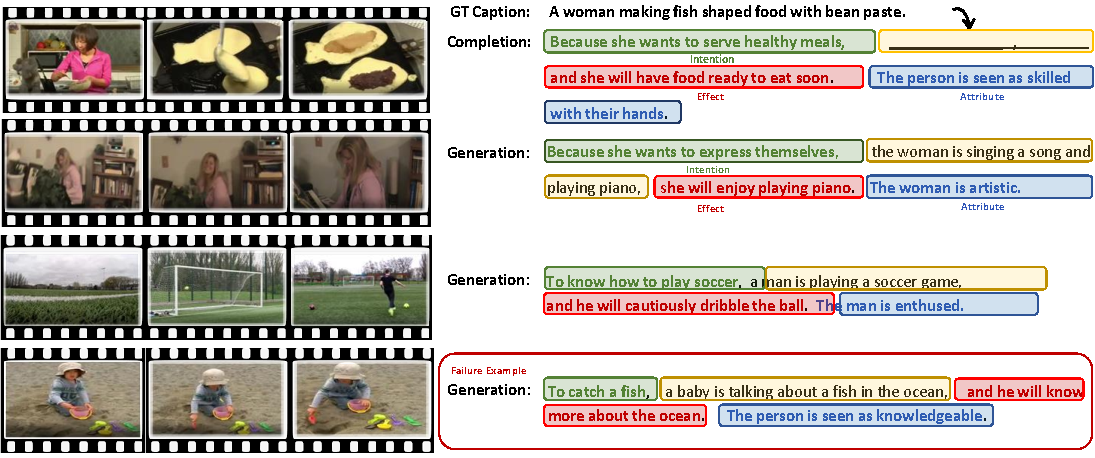
\includegraphics[width=\linewidth]{./v2c/fig/qualitative.pdf}
        \caption{Examples of outputs of our model for the V2C Completion and Generation tasks along with the ground-truth (GT) caption.
        A failure example shown in the bottom red box. }
        \label{fig:qualitative}
    \end{figure*}  
    
    
    \paragraph{Human Evaluation}
    In Table~\ref{tab:humanevaluation}, {E2C} (Event to Commonsense) is the task of commonsense completion given only textual events~\cite{sap2018atomic,bosselut2019comet} as opposed to V2C which uses both text and video.
    9E\textsc{nc}9D\textsc{ec}~\cite{sap2018atomic} is composed of nine GRU based encoder-decoders as a baseline model for commonsense completion on text, and C\textsc{omet}~\cite{bosselut2019comet} is a large-scale generative pre-trained transformer (GPT) model~\cite{radford2018improving}. 
    We would like to highlight that our transformer model is light-weight with only half of the parameters in GPT without any pre-training. 
    
    We evaluate our model on the tasks of caption generation with human evaluations, and also compare it with the gold annotations. 
    Our gold annotation for ground-truth captions (sourced from the MSR-VTT dataset) points to the fact that a small percentage of captions from MSR-VTT are not relevant to the video, and this is amended by our human workers.
     
    For the  {V2C-Completion} task, our V2C-Transformer model is substantially better (by 7.73\%) than the LSTM-based model from \cite{gao2017video}, and shows consistent lead on each dimension. 
    Thus, when the ground-truth caption is given, our model is able to generate much more relevant commonsense descriptions, thereby consolidating it's ability of commonsense generation.
    
    For the task of  {V2C-Generation}, the difference between human scores for LSTM vs V2C-Transformer is reduced, but our VTC outperforms on average by 2.98\%.
    This may be attributed to the fact that the LSTM-based model is slightly better at generating captions.
   

    \paragraph{Generating Textual Stories with Commonsense}
    In order to generate story-like textual descriptions that complement the factual captions, we additionally train our model to exploit our diverse complete-sentence annotations.
    Specifically, instead of producing the commonsense knowledge given the videos and captions, we finetune our pre-trained V2C-Transformer model on predicting the human rewritten texts, and generate complete story-like captions.
    Since we do not have enough annotations per sample to compute a fair BLEU score for comparisons, we showcase some sample generated descriptions for qualitative analysis (see Figure~\ref{fig:qualitative}). 
    With that, we observe V2C-Transformer is able to produce complete stories that contain simple, while logically consistent storylines that complement both the visual content and the factual descriptions. 
    We believe that collecting a set of story-like sentences will further enrich our models, and allow us to generate much more contextual, creative, and natural commonsense descriptions from a video. 


\section{V2C-QA}
\begin{figure}[t]
    \centering
    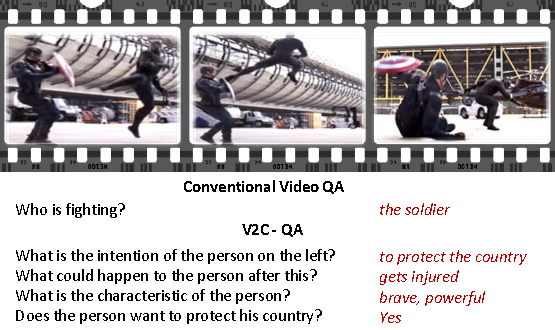
\includegraphics[width=\linewidth]{v2c/fig/v2cqa.pdf}
    \caption{Example questions from V2C-QA compared with conventional video question answering.}
    \label{fig:v2cqa}
\end{figure}
Another way of generating commonsense descriptions about the video is by asking pointed questions.
Consider the example in~\ref{fig:pipeline} where we ask the question \textit{``What happens next to the runners"}, about the \textit{effect} of the action ``prepare" performed by the agents \textit{``group of runners"} observed in the video.
We propose a V2C-QA -- an open-ended commonsense video question-answering task, where we ask questions about the intents, effects and attributes of the agents in the video.

\noindent\textbf{Dataset:}
We use the caption and commonsense annotations in the V2C dataset to create question-answer pairs for each video.
We first extract the action and subject from the caption using SpaCy linguistic features~\cite{honnibal-johnson:2015:EMNLP}.
For each intention, attribute and effect for a video, we use template-based generation to get 7 types of questions -- yielding 21 questions per sample, including negative questions as in~\citet{gokhale2020vqa}.
In total, we have 1,250 training videos and 250 test videos, and a total of 37k questions.
We have a set of 5,555 unique answers for our questions.
Each question can have multiple possible true answers as shown in the example in Figure~\ref{fig:v2cqa}.
The V2C-QA task asks questions that require commonsense reasoning about internal mental states, motivations, and latent aspects of agents in the video as opposed to the conventional video-QA questions about visible objects and actions.


\paragraph{Models:}
We utilize our V2C-Encoder followed by an open-ended answering module.
We jointly predict the type of the question and combine it with the V2C encoding using a feed-forward network.
For textual features, we use embeddings from BERT-base~\cite{devlin2018bert}.
Our models are trained on the open-ended QA task and set-up as a multi-label classification task similar to VQA~\cite{antol2015vqa}, with an answering module design inspired by LXMERT~\cite{tan2019lxmert}.
Our loss function includes the classification loss for answering, the attention loss for question-type, and a label-ranking loss.

    \begin{table}[t]
        
        \centering
        \resizebox{\linewidth}{!}{
        \begin{tabular}{@{}p{0.45mm}p{3.77cm} p{0.65cm}p{0.65cm} p{0.65cm}p{0.65cm} p{0.65cm}p{0.65cm}}
            \toprule 
            % \multirow{2}{*}{\textbf{Type}} 
            & \multirow{2}{*}{\textbf{Model}} 
            & \multicolumn{2}{c}{\textbf{top-1}}   
            & \multicolumn{2}{c}{\textbf{top-3}}   
            & \multicolumn{2}{c}{\textbf{top-5}} 
            %   & \multirow{2}{*}{\pbox{18mm}{Ranking Loss}}
            \\
            \cmidrule{3-4} \cmidrule{5-6} \cmidrule{7-8}
            & & p & r & p & r & p & r\\
            
            \toprule 
            \multirow{5}{*}{\rotatebox{90}{\textbf{Intention}}} 
            & MSR-VTT QA        & 9.68 & 2.13 & 7.15 & 4.68 & 6.07 &  6.60\\
            & V2C-T             & 10.34 & 2.31 & 7.69 & 5.03 & 6.37 & 6.87\\
            & V2C-T + Captions  & 10.72 & 2.54 & \textbf{8.08} & 5.47 & 6.39 & 7.20\\
            & Pretrained V2C-T  & 10.77 & \textbf{2.69} & 8.01 & 5.58 & \textbf{6.71} & 7.88\\
            & Pretrained V2C-T~+~Cap. & \textbf{11.04} & 2.68 & 7.96 & \textbf{5.70} & 6.63 &\textbf{7.79}\\
            
            \midrule 
            
            \multirow{5}{*}{\rotatebox{90}{\textbf{Effect}}} & MSR-VTT QA & 19.89 & 5.02 & 8.04 & 5.91 & 5.30 & 6.49\\
            & V2C-T & 20.95 & 5.43 & 8.65 & 6.57 & 5.65 & 7.06\\
            & V2C-T + Captions  & 20.95 & 5.32 & 8.50 & 6.48 & 5.76 & 7.26\\
            & Pretrained V2C-T & 20.95 & 5.32 & 8.63 & 6.55 & 5.82 & 7.49\\
            & Pretrained V2C-T~+~Cap. & \textbf{21.12} & \textbf{5.60} & \textbf{8.70} & \textbf{6.89} & \textbf{5.83} & \textbf{7.68}\\
            \midrule
            
            \multirow{5}{*}{\rotatebox{90}{\textbf{Attribute}}} & MSR-VTT QA & 46.10 & 37.22 & 16.02 & 49.45 & 7.49 & 41.03\\
            & V2C-T & 59.52 & 48.30 & 22.39 & 51.40 & 13.97 & 52.57\\
            & V2C-T + Captions & 59.74 & 48.22 & 23.12 & 52.44 & 14.64 & 54.35\\
            & Pretrained V2C-T & \textbf{60.72} & \textbf{49.00} & \textbf{23.18} & \textbf{52.73} & \textbf{14.98} & \textbf{55.40}\\
            & Pretrained V2C-T +Cap. & 59.57 & 48.24 & 23.10 & 52.54 & 14.94 & 54.91\\
            \midrule 
            & Text-Only Baseline & 12.36 & 11.70 & 13.84 & 12.35 & 14.77 & 14.10 \\
            
            \bottomrule
        \end{tabular}
        }
        \caption{Precision (p) and Recall (r) for V2C-QA for each type of question. 
        % The best-performing model for each description category and task is given in bold, while the overall best is underlined
        }
        \label{tab:v2cqa_results}
    \end{table} 
\paragraph{Results:}
MSR-VTT QA~\cite{xu2017video} is as a good baseline since it is trained on a conventional videoQA task on the MSR-VTT videos, and only takes video and query as input, unlike recent video understanding models~\cite{lei2018tvqa} that take additional supervision, such as subtitles.
However this model is trained for a multiple-choice QA scheme, so we modify it with our open-ended answering module.
We compare our models when we use our encoder pretrained on the V2C caption generation task, and then finetune it on the V2C-QA task.
We also train models with ground-truth factual captions as input.
Our results are shown in Table~\ref{tab:v2cqa_results}, where we evaluate on prediction of top-k (1,3,5) answers, and report precision and recall.
Our encoder pre-trained on the V2C task outperforms all other models.
Attribute-related questions are easier to answer, while the models struggle the most for questions about intention. Captions help in questions about effects.
The overall text-only baseline shows an insignificant bias between the question and answer-options.

\section{Related Work}
    \noindent\textbf{Video Captioning:}
    Captioning is crucial for understanding visuals; however it is typically limited to describing observable objects and events~\cite{yang2011corpus,thomason2014integrating,gan2017semantic}),
    or for generating paragraphs or multi-sentence captions about the image or video~\cite{krause2016paragraphs,krishna2017dense}.
    However, for detailed video understanding, one needs to obtain descriptions that go beyond observable visual entities and use background knowledge and commonsense to reason about objects and actions.
    Work for inferring motivations of human actions in static images by incorporating commonsense knowledge are reflected in~\citet{pirsiavash2014inferring,vondrick2016predicting}.
    Commonsense caption generation has been approached on abstract scenes and clip-art images in~\citet{vedantamLinICCV15}.
    We present the first generative model for commonsense video captioning.
    
    \noindent\textbf{Video Question Answering:}
    Since caption generation can only describe observable events, recent work seeks to move closer to comprehension, by learning to answer complex questions about videos.
    However, the datasets used for Video QA~\citep{yang2003videoqa,xu2016msr,zhu2017uncovering} focus only on directly evident visual concepts and construct the questions mostly about ``where'' and ``what'' aspects.
    Question answering on movie videos has been explored by~\citet{tapaswi2016movieqa} who collect questions about ``why'' and ``how'' aspects.
    Recently~\citet{lei2018tvqa,zadeh2019social} have propose video-based QA tasks with open-ended high-order questions that need multi-modal understanding, social intelligence modeling, and spatio-temporal reasoning.
    We introduce a novel open-ended video question answering task in this paper, where the questions are about three aspects of commonsense human behavior.

    \noindent\textbf{Visual Reasoning:}    Aspects of visual reasoning have been explored by~\citet{yatskar2016situation} as a situation recognition task on single images, and in Visual Madlibs~\citep{yu2015visual} as a ``fill-in-the-blanks" task for single-image captioning that contains some categories which require reasoning about internal mental states and future events.
    \citet{kim2018textual} provide textual explanations for actions in a self-driving scene.
    \citet{zellers2019recognition} propose a visual question answering task that requires commonsense reasoning to answer a question and to provide a rationale behind the answer.
    Spatial and compositional reasoning is required to answer questions about synthetic images in CLEVR~\cite{johnson2017clevr}. Critical aspects of visual reasoning also include the model's ability to conduct object grounding by natural language descriptions~\citep{rohrbach2016grounding,fang2018weakly,fang2019modularized}.
    Another aspect of visual reasoning is the ability predict a sequence of actions (procedure planning), or to reason about intermediate video frames (walkthrough planning) between two frames, explored in \citet{gokhale2019blocksworld,chang2019procedure}.
    
    \noindent\textbf{Textual Commonsense:}
    Commonsense-based question answering is an area of active research with several datasets and challenges requiring reasoning about conceptual commonsense~\cite{talmor2019commonsenseqa}, physical commonsense~\citep{bisk2020piqa}, social commonsense~\citep{sap2019social}, and abductive commonsense~\citep{bhagavatula2020abductive}.
    On the other hand, challenges such as ProPara~\citep{mishra2018tracking} and bAbI~\citep{weston2015towards} require tracking elements, actions, and effects of actions.
    Commonsense-based text generation has recently been explored via the A\textsc{tomic} dataset~\cite{sap2018atomic}, a corpus of 877k textual descriptions of inferential knowledge organized as \textit{if-then} relations.
    \citet{bosselut2019comet} adopt the A\textsc{tomic} dataset to learn a generative model of commonsense knowledge.
    To the best of our knowledge, ours is the first work on \textit{generating} commonsense descriptions from visual inputs.


\section{Outlook}
A video typically contains one or many objects (sometimes performing actions) in different backgrounds, scenes, or situations.
Some objects may be ``passive" such as trees or buildings, while some objects may be ``active" such as people performing actions like walking, singing, and driving.
This paper is focused on describing such active agents in terms of their intentions, effects of their actions, and attributes that characterize these agents.

We distinguish V2C from the traditional video captioning task.
Video captions describe observable objects, background, and actions, while commonsense descriptions in our task seek to describe the unobservable intentions of the agent (pre-conditions or mental conditions), effects of the action (that happen in the future), and attributes which characterize the agent.
Thus commonsense generation goes \textit{beyond the visible}.
Ours is the first attempt at developing a generative video-based commonsense model.
We anticipate that our framework can be utilized for many applications in video understanding, comprehension, human-robot interaction, and learning commonsense in a multi-modal setting.


\section{Conclusion}
In this paper, we explore a novel and challenging task to generate video descriptions with rich commonsense descriptions that complement the factual captions.
We expand an existing video captioning dataset for the V2C task through automated retrieval from a textual commonsense corpus followed by human labeling, and present a novel V2C-Transformer model to serve as a strong baseline method for the V2C task. 
Our evaluation verifies the effectiveness of our method, while also indicating a scope for further study, enhancement, and extensions in the future. 
Our experiments on using the V2C-Transformer as a component for the V2C-QA task show that the model has transfer learning capabilities that can be applied to other vision-and-language tasks such as question-answering, that require commonsense reasoning.

% \section*{Acknowledgements}
% {
% The authors acknowledge support from the NSF Robust Intelligence Program project \#1816039, the DARPA KAIROS program (LESTAT project), the DARPA SAIL-ON program, and ONR award N00014-20-1-2332.
% ZF, TG, YY thank the organizers and the participants of the   \href{https://sites.google.com/view/telluride2019/}{Telluride Neuromorphic Cognition Workshop}, especially the Machine Common Sense (MCS) group.
% }
% \bibliography{emnlp2020}
% \bibliographystyle{acl_natbib}

% \clearpage
% \appendix
% \input{supp}

% \chapter{Adversarially Learned Transformations for Single-Source Domain Generalization}
\label{chap:alt}
In Chapter~\ref{chap:agat}, we looked at a relaxed setting of the generalization problem -- in that setting, information about the target domain was available in terms of a set of attributes that are known to differ at test time.
% (target samples are not available).
In this chapter we will go beyond attributes and address the harder and broader problem of domain generalization.

% As discussed earlier, domain generalization is the problem of making accurate predictions on previously unseen domains, especially when these domains are very different from the data distribution on which the model was trained. 
% In this chapter, we will tackle an even harder problem -- \textit{single source domain generalization (SSDG)}, where the model has access only to a single training domain, and is expected to generalize to multiple different testing domains. 
% This is especially hard because of the limited information available to train the model with just a single source. 

% \section{Introduction}
\begin{figure}
    \centering
    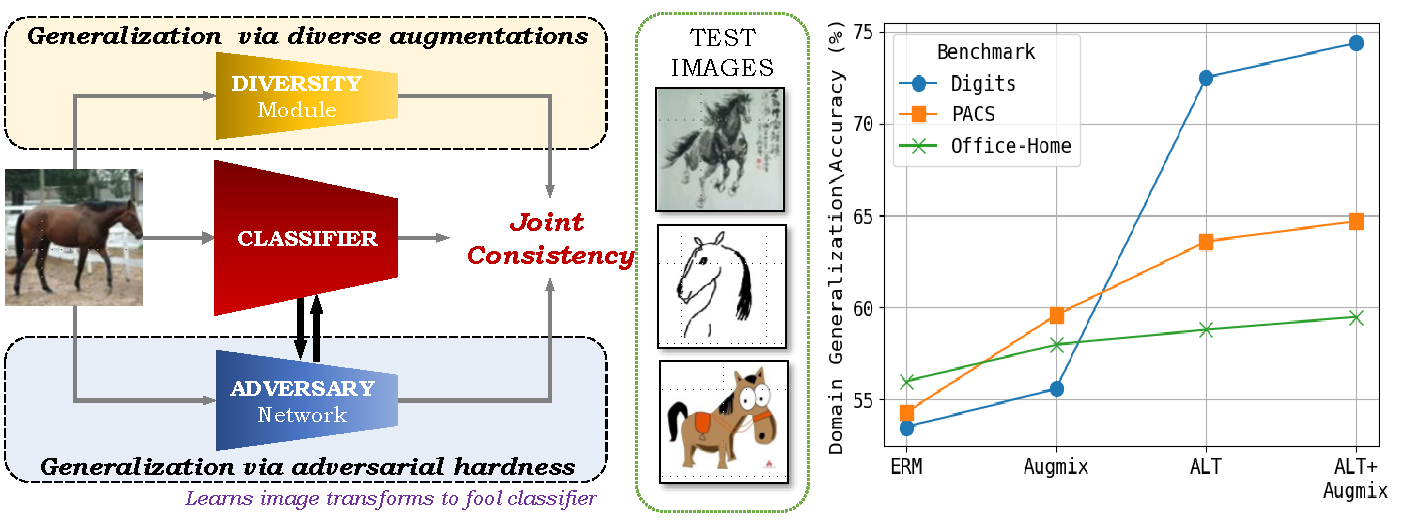
\includegraphics[width=\linewidth]{alt/figures/alt_teaser.pdf}
    \caption{
    This figure illustrates our approach which consists of a \textit{diversity} module (data augmentation functions such as Augmix~\citep{hendrycks2019augmix} or RandConv~\citep{xu2020robust}) and an \textit{adversary} network (ALT) (to learn image transformations that fool the classifier).
    We show an example from the PACS benchmark under the single-source domain generalization setting, with real photos (P) as the source domain and art paintings (A), cartoons (C), and sketches (S) as the target domains.
    The plot summarizes our results -- while diversity alone improves performance over the naive ERM baseline, adapting this diversity using adversarially learned transformations (ALT) provides a significant boost for domain generalization on multiple benchmarks.}
    \label{fig:alt_teaser}
\end{figure}


Domain generalization is the problem of making accurate predictions on previously unseen domains, especially when these domains are very different from the data distribution on which the model was trained. 
This is a challenging problem that has seen steady progress over the last few years \citep{carlucci2019domain,volpi2018generalizing,qiao2020learning,xu2020robust,nam2021reducing}. 
this chapter focuses on the special case -- single source domain generalization (SSDG) -- where the model has access only to a single training domain, and is expected to generalize to multiple different testing domains. 
This is especially hard because of the limited information available to train the model with just a single source. 

In the case where multiple training domains (i.e., multi-source DG) are available, recent analysis \citep{gulrajani2021in} shows that even simple methods like minimizing empirical risk jointly on all domains, performs better than most existing sophisticated formulations.
% on par with sophisticated formulations.
A corollary to this finding is that success in 
%SSDG
domain generalization is primarily dependent on \emph{diversity} -- i.e., exposing the model to as many potential training domains as possible.
As the SSDG problem allows access only to a single training domain, such an exposure must come in the form of diverse transformations of the source domain that can simulate the presence of multiple diverse domains ultimately leading to low generalization error. 
% which in this case must be in the form of diverse transformations of the source domain that can simulate the presence of multiple different domains ultimately leading to low generalization error. 

The idea of using diversity to train better models has been sufficiently explored -- many recent approaches have shown that a diverse set of augmentations during training improves a model's robustness under distribution shifts \citep{hendrycks2019augmix,yun2019cutmix,zhang2018mixup,cubuk2020randaugment}. 
However, the extent to which the model needs to be exposed to the diverse transformations is unclear, and over-exposure may hurt the model's generalization capabilities. 
Moreover, these methods define a strong prior in terms of the types of diversity that is desirable -- for e.g., in object recognition tasks, invariance to affine transformations, color jitter, blurs, or other kinds of pixel noise is desirable. 
Specific augmentations can be used if the type of diversity encountered at test time is known; for instance if it is known that the test set may contain random combinations of rotation, translation, and scaling, using augmentations that are correlated with this domain shift would lead good performance~\citep{gokhale2021attribute,benton2020learning,wong2020learning}.

Unfortunately, by design, these methods can only achieve invariance under small distribution shifts, like unknown corruptions, noise or imperceptible and perceptible adversarial attacks. 
These methods typically do not work effectively when the distribution shift is large and of a semantic nature, as in the case of domain generalization. 
On the other hand, some recent methods have directly used randomized convolutions to synthesize diverse image manipulations~\citep{xu2020robust}, motivated by the large space of potentially realizable functions induced by a convolutional layer, which cannot be easily emulated using simple analytical functions. 
 
In this chapter we hypothesize that, while diversity is critical in order to succeed in single domain generalization, diversity alone is insufficient. 
In other words, blindly exposing a model to a wide range of transformations cannot improve the generalization performance. Instead, we argue that other carefully designed forms of diversity are needed -- specifically those that can expose the model to unique, and task-dependent transformations with large semantic changes that are otherwise unrealizable with plug-and-play augmentations as before.  To this end, we introduce an adversary network whose objective is to find plausible image transformations that maximize classification error. We enforce a consistency between a \textbf{diversity module} and the \textbf{adversary network} during training along with the classifier's predictions. 

Our method, dubbed ALT (adversarially learned transformations), offers an interplay between diversity and adversity. Over time, a synergistic partnership between the diversity and adversary networks emerges, exposing the model to increasingly unique, challenging and semantically diverse examples that are ideally suited for single source domain generalization.  The adversary network benefits from the classifier being exposed to the diversity module, and as such avoid trivial adversarial samples with appropriate checks. This allows the adversarial maximization to explore a wider space of adversarial transformations that cannot be covered by prior work on pixel-level additive perturbations.
  
We demonstrate this advantage of our method empirically on multiple benchmarks -- PACS \citep{li2017deeper}, Office-Home \citep{venkateswara2017deep}, and Digits \citep{volpi2018generalizing}. On each benchmark, we outperform the state-of-the-art single source domain generalization methods by a significant margin.  Moreover, since our framework disentangles diversity and adversarial modules, we can combine it with various diversity enforcing techniques -- we identify two such state-of-the-art methods with AugMix \citep{hendrycks2019augmix}, and RandConv \citep{xu2020robust}, and show that placing them inside our framework leads to significantly improved generalization performance over their vanilla counterparts. 
We illustrate this idea in figure \ref{fig:alt_teaser} where we show an image of a horse from the 'photo' training distribution in PACS and the different styles of cartoon/sketch/art painting horses that may be encountered at test time. 

\paragraph{Contributions:}
We summarize our contributions below:
\begin{itemize}[nosep,noitemsep,leftmargin=*]
    \item We introduce a method, dubbed ALT, which produces adversarially learned image transformations that expose a classifier to a large space of image transformations for superior domain generalization performance. ALT performs adversarial training in the parameter space of an adversary network as opposed to pixel-level adversarial training.
    \item We show how ALT integrates diversity-inducing data augmentation and hardness-inducing adversarial training in a synergistic pipeline, leading to diverse transformations that cannot be realized by blind augmentation strategies or adversarial training methods on their own.
    \item We validate our methods empirically on three benchmarks demonstrating state-of-the-art performance, and provide insights into and analysis of approach.
\end{itemize}

% Instead, the model must be able to trade-off diversity and classifier performance as needed such that it achieves 'optimal' exposure in a given task, and no more --  which is challenging to define \emph{a priori}. Instead, we are able to achieve this trade-off using a consistency using an additional network that acts an adversary to the classifier by learning adversarial transformations of the input image for every single batch during training. By randomly initializing this network in each iteration, we ensure the adversarial transformations are unique, and diverse themselves. We then place a consistency objective between the diverse and adversarial transformations so together they expose the model to learn from both diverse and challenging domains
% \section{Related Work}
\textbf{Domain Generalization}
has been explored under both multi-source (MSDG) and single-source (SSDG) settings. Techniques designed for MSDG seek to utilize the multiple domains to perform feature fusion~\citep{shen2019situational}, learning domain-invariant features~\citep{ganin2016domain}, meta-learning~\citep{li2018learning}, invariant risk minimization~\citep{arjovsky2019invariant}, learning mappings between multiple training domains~\citep{robey2021model}, and style randomization~\citep{nam2021reducing}.
Gulrajani  \textit{et al.}~\citep{gulrajani2021in} provide an extensive comparative study of these approaches and report that simply performing ERM on the combination of source domains leads to the best performance. Many benchmarks have been proposed to evaluate MSDG performance such as PACS~\citep{li2017deeper}, OfficeHome~\citep{venkateswara2017deep}, Digits~\citep{volpi2018generalizing}, and WILDS~\citep{koh2021wilds} which is a compendium of MSDG datasets for various tasks such as image classification, text sentiment classification, text toxicity prediction, etc. In the context of multi-source DG, \citep{zhou2020learning} propose to synthesize novel domains using a conditional generator trained on multiple domains using cycle consistency -- whereas we are primarily interested in the single source setting where such a method may not be feasible. Moreover, we strictly synthesize novel domains as functions of the source domain, and place emphasis on the nature of functions that are learnable during training with a convolutional network with objectives such as an adversarial cost and consistency measures.

SSDG is a harder setting due to the lack of multiple datasets for using the above methods; most work in SSDG has therefore focused on data augmentation.
Notable among these methods is the idea of adversarial data augmentation -- ADA\citep{volpi2018generalizing} and M-ADA~\citep{qiao2020learning} apply pixel-level additive perturbations to the image in order to fool the classifier.  Resulting images are used as augmented data to train the classifier.
% is trained over the union of source dataset and adversarial samples.
RandConv~\citep{xu2020robust} shows that shape-preserving transformations in the form of random convolutions of images lead to impressive performance gains on Digits.
% benchmark.

\textbf{Robustness to Image Corruptions.}
There has also been interest in training classifiers that are robust to corruptions that occur in the real world, such as different types of noise and blur, artifacts due to compression techniques, and weather-related environments such as fog, rain, and snow.
\citep{vasiljevic2016examining,geirhos2018generalisation} show that training models with particular types of corruption augmentations does not guarantee robustness to other unseen types of corruptions or even different severities of corruptions. 
Hendrycks~ \textit{et al.}~\citep{hendrycks2018benchmarking} curate benchmarks (ImageNet-C and CIFAR-C) to test robustness along a fixed set of corruptions.
They also provide a benchmark called ImageNet-P which tests robustness against other corruption types such as small tilts and changes in brightness.
A similar benchmark for corruptions of handwritten digit images, MNIST-C~\citep{mu2019mnist} has also been introduced.

% \paragraph{Robustness to Adversarial Attacks}

\textbf{Data Augmentation}
has been an effective strategy for improving in-domain generalization using simple techniques such as random horizontal flips and cropping~\citep{he2016deep}, random occlusion or removal of patches~\citep{devries2017improved,zhong2020random}.
Data augmentation techniques have been shown to improve robustness against adversarial attacks and natural image corruptions~\citep{zhang2018mixup,yun2019cutmix,cubuk2020randaugment}.
Learning to augment data has been explored in the context of object detection~\citep{zoph2020learning} and image classification~\citep{ratner2017learning,cubuk2019autoaugment,zhang2019adversarial}. 
% - previous methods for SSDG: naive data aug, 

% - style changes, style normalization 

% - diversity: augmix, randconv, older random projection papers, 

% - adversarial data aug --- talk about how adv training can only provide resiliency to small perturbations 

%  - newer methods when some info is known about target (but no dataset available) -- agat, perturbation sets rts

\section{Proposed Approach} 
% \paragraph{Preliminaries.}
Under the single-source domain generalization setting, consider the training dataset $\mathcal{D}$ containing $N$ image-label pairs $\mathcal{D} = \{(\xx_i, \yy_i)\}_{i=1}^{N}$, and a classifier $f$ parameterized by neural network weights $\theta$. 
The standard expected risk minimization (ERM) approach seeks to learn $\theta$ by minimizing the the in-domain risk measured by a suitable loss function such as the binary cross-entropy loss.
\begin{equation}
    \mathcal{R}_{ERM} = \underset{\xx\in\mathcal{D}}{\E} \mathcal{L}_{BCE}(f(\xx;\theta), \yy).
    \label{alt:eq:erm}
\end{equation}
For SSDG, we are interested in a classifier that has the least risk on any \textit{unseen} target domain $\mathcal{D}^\prime$ that is not observed during training. Note that in SSDG, there is only domain shift and no label shift, i.e. we assume the same classes exist in the training and testing domains. 
Our approach builds on diversity based and adversarial augmentation approaches which we outline next. 

\paragraph{Generalization via Diversity.} A successful strategy to improve generalization error on unseen domains is to utilize a diverse set of pre-defined transformations, $\mathcal{F}_{div}$, to synthesize data augmentations that emphasize the invariance properties that are important for $f(\theta)$ to learn. Methods that fall under this category modify Equation \ref{alt:eq:erm} as follows: 
\begin{equation}
    \label{alt:eq:div_erm}
    \mathcal{R}_{div} = \underset{\xx\in\mathcal{D}}{\E} \mathcal{L}_{BCE}(f(\xx; \theta), \yy) + \lambda_{KL} D_{KL},
\end{equation}
where $D_{KL}$ is a consistency term, typically a divergence, such as KL-Divergence, between the softmax probabilities of the classifier obtained with the clean and transformed data, respectively, \textit{e.g.}, $D_{KL} = KL(f(\xx) ||f(\mathcal{F}_{div}(\xx)))$. 
When $\mathcal{F}_{div}$ is chosen as a set of pre-defined transformations like shear, rotate, color jitter etc., this approach is referred to as AugMix \citep{hendrycks2019augmix}, and when it is a set of randomly initialized convolutional layers this method becomes RandConv \citep{xu2020robust} -- both of which are among the most effective strategies to enforce diversity-based consistencies for generalization.
Although these methods have the advantage of being simple pre-defined transformations that are dataset agnostic, they suffer from drawbacks under the SSDG setting.
When executed on their own, they may not capture sufficient diversity in terms of \textbf{large} semantic shifts, such as when expecting generalization on sketches from a model trained on photos.
% However, these methods suffer from a few drawbacks -- they are pre-defined and capture a large class of potential image transformations (particularly rand-conv), but when executed on their own, they may not capture sufficient diversity in terms of \emph{large} semantic shifts. 

\paragraph{Generalization via adversarial hardness.}
An alternative approach to domain generalization is via adversarial augmentation  which exposes a classifier to `hard' samples during training -- defined broadly as examples that are carefully designed to cause the model to fail. Such samples are augmented to the training set, with the expectation that exposure to such adversarial examples can improve the model's generalization performance on unseen domains \citep{volpi2018generalizing,qiao2020learning}. This is commonly enforced by learning an additive noise vector which when added, maximizes classifier cost. Unfortunately in the case of domain generalization, these methods have failed to match the performance of diversity-only methods optimizing for the cost outlined in Equation~\ref{alt:eq:div_erm}. This is in part because they lack sufficient diversity, and by design they can only guarantee robustness to small perturbations from the training domain, as opposed to large semantic shifts, which are crucial for domain generalization.

% \begin{equation}
%     \label{alt:eq:div_erm}
%     \mathcal{R}_{adv} = \underset{||\delta||_p < \epsilon}{\textrm{max}}~\mathcal{L}_{BCE}(f(\xx+\delta;\phi); \theta), \yy)
% \end{equation}

\begin{algorithm}[t]
    \caption{Adaptive Diversity via ALT}
    \begin{algorithmic}[0]
        \State \textbf{Input:} Source dataset $\mathcal{D}=\{(\xx_i,\yy_i)\}_{i=1}^N$ 
        \State \textbf{Output:} Learned weights $\theta^*$  
    \end{algorithmic}
    \begin{algorithmic}[1]
        \State \textbf{Initialize:} $\theta\gets\theta_0$ \algorithmiccomment{weights of $f()$}
        \ForEach{$t \in \{1\dots T\}$}%
            \State $\xx_t, \yy_t \sim\mathcal{D}$ \algorithmiccomment{\textit{sample input batch}}
            % \Statex ~~\quad$\triangleright$~\textit{train on source only}
            \If{$t < T_{pre}$} 
                \State $\theta\gets\theta - \eta\nabla \mathcal{L}_{cls}(f(\xx_t;\theta), \yy_t))$ 
            % \Statex ~~\quad$\triangleright$~\textit{ALT}
            \Else
                \State $\rho\gets\rho_0,~\phi\gets\phi_0$\algorithmiccomment{weights of $r()$, $g()$}
                \ForEach{$i\in{1\dots m_{adv}}$}
                    % \State $\phi\sim KN()$ \algorithmiccomment{initialize $\phi$}
                    % \State $\hat{\yy}\gets f(\xx; \theta)$
                    % \State $\xx_g \gets g(\xx;\phi)$
                    \State $\hat{\yy_g} \gets f(g(\xx;\phi);\theta)$
                    % \State $L_{adv} \gets \mathcal{L}_{cls}(\hat{\yy_g}, \yy) - \mathcal{L}_{TV}(\xx_g)$
                    % \State $\phi\gets\phi+\nabla\mathcal{L}_{adv}$
                    \State $\phi\gets\phi+\nabla(\mathcal{L}_{cls}(\hat{\yy_g}, \yy) - \mathcal{L}_{TV}(\xx_g))$
                \EndForEach
                % \Statex ~~\quad~~\quad $\triangleright$ \textit{Consistency}
                % \State $p_c,~p_r,~p_g \gets f(\xx; \theta),~f(r(\xx); \theta),~f(g(\xx); \theta)$
                % \State $p_{mix}\gets (p_c + w_r p_r + (2-w_r)p_g)/3$
                % \State $\mathcal{L}_{KL}\gets\sum_{j\in\{c,r,g\}}D_{KL}(p_{mix}||p_j)$ 
                % \State $\theta\gets\theta-\eta_{adv}\nabla((1-\lambda_{KL})\mathcal{L}_{cls} + \lambda_{KL}\mathcal{L}_{KL})$
                \State $\theta\gets\theta-\eta_{adv}\nabla\mathcal{L}_{ALT}$ \algorithmiccomment{see Eq.\ref{alt:eq:L_KL},\ref{alt:eq:L_ALT}}
            \EndIf 
        \EndForEach
        \State\Return $\theta$
\end{algorithmic}
\label{algo}
\end{algorithm}



\paragraph{Adversarially Learned Transformations (ALT).}
While diversity-only methods have shown promise, they are limited in their ability to generalize to domains with large semantic shifts; on the  other hand, techniques based purely on adversarial hardness are theoretically well-motivated but do not match the performance of diversity-based methods. Instead, in this chapter, we propose a new approach that takes the best of these two approaches using an adversary network that is trained to create \emph{plausible} image transformations that fool the classifier. These manipulated images are then used during training as examples on which the image must learn invariance. Since these perturbations are parameterized as learnable weights of a neural network, the network is free to choose large, complex transformations without being restricted to additive noise as done in previous work~\citep{volpi2018generalizing}. Further, this network is randomly initialized for each batch, making the types of adversarial transformations discovered unique and diverse over the course of training.  
%
% With this goal in mind, we propose learning transformations of source images using an adversarially trained image-to-image transformation network 

Formally, the adversary network transforms the input image as $g\colon\R^{C\times H\times W}\rightarrow\R^{C\times H\times W}$, where $C$, $H$, $W$ are the number of channels, height, and width of input images.
$g$ is parameterized by a set of weights denoted by $\phi$. This network, dubbed ALT, forms the backbone of our method.  To train ALT, we setup an adversarial optimization problem with the goal of producing transformations, which when applied to the source domain, can fool the classifier $f$.
While existing efforts dealing with robustness to small corruptions use pixel-level and $\ell_p$ norm-bounded perturbations to fool the model, we find that this is not sufficient for domain generalization as such methods do not allow searching for adversarial samples with semantic changes.
Instead, we directly perform adversarial training in the space of $\phi$, i.e., the neural network weights of ALT. Given input images $\xx$, parameters $\phi$ are randomly initialized, and the corresponding adversarial samples $\xx_g$ are found as:
\begin{equation}
    \xx_g = \underset{\phi}{\textrm{max}}~\mathcal{L}_{BCE}(f(g(\xx;\phi); \theta), \yy) - \mathcal{L}_{TV}(g(\xx;\phi)). 
    \label{alt:eq:adv_max}
\end{equation}
The first term seeks to update $\phi$ so as to maximizes the classifier loss, while $\mathcal{L}_{TV}$ (total variation)~\citep{rudin1992nonlinear} acts as a smoothness regularization for the generated image $\xx_g = g(\xx;\phi)$. The maximization in Equation \ref{alt:eq:adv_max} is solved by performing $m_{adv}$ steps of gradient descent with learning rate $\eta_{adv}$. We note a few important aspects of ALT -- unlike existing methods that explicitly place an $\ell_p-$norm constraint on the adversarial perturbations, we control the strength of the adversarial examples by limiting the number of optimization steps taken by $g$ to maximize classification error. Next, since we randomly initialize $g$ for each batch, the network is reset to a random function. In fact, when the number of adversarial steps is set to 0, $g$ behaves similar to RandConv \citep{xu2020robust} since its only a set of convolutional layers, with additional non-linearity. Finally, in addition to limiting the number of adversarial steps, we place a simple total variation loss on the generated image to force smoothness in the output. This naturally suppresses high frequency noise-like artifacts and encourages realistic image transformations and prevents the network from learning trivial transformations  -- for e.g., only noise or removing semantic content entirely. 

\paragraph{Improving Diversity.}
The samples $\xx_g$ obtained by solving Equation~\ref{alt:eq:adv_max} represent hard adversarial images that can be leveraged by the model to generalize to domain shift. But it also lends itself to exploit other forms of na\"ive diversity achieved by methods like RandConv and AugMix.
% On the other hand, augmentations such as RandConv and Augmix produce images that represent predefined image transformations such as random scaling, cropping, affine transformations, color jitter and so on.
We represent these ``diversity modules'' as $r$, which produce outputs $\xx_r{=}r(\xx)$. Our method utilizes these samples in the training process by enforcing a consistency between the predictions of the classifier on the source image and its transformations from $r$ and $g$. By including the diversity module into the optimization process, the invariances inferred by the classifier lead to stronger and more diverse adversarial examples in future epochs. 
Eventually, a synergistic partnership emerges between the diversity module and the adversary network to produce a wide range of image transformations that are significantly different from the source domain.  

Let $p_c$, $p_r$, and $p_g$ denote the softmax prediction probabilities of classifier $f$ on $\xx$, $\xx_r$, and $\xx_g$, respectively. Then the consistency between these predictions can be computed using Kullback-Leibler divergence~\citep{kullback1951information} as:
\begin{equation}
    \mathcal{L}_{KL} = D_{KL}(p_{mix}||p_c) + w_r D_{KL}(p_{mix}||p_r) + (2-w_r) D_{KL}(p_{mix}||p_g), 
    \label{alt:eq:L_KL}
\end{equation}
% \begin{equation}
%     \mathcal{L}_{KL} = D_{KL}(p_{mix}||p_c) + w_r D_{KL}(p_{mix}||p_r) 
%     % \nonumber\\
%     + (2-w_r) D_{KL}(p_{mix}||p_g), 
%     \label{alt:eq:L_KL}
% \end{equation}
where $p_{mix}$ denotes the mixed prediction:
\begin{equation}
    p_{mix} = \frac{p_c + w_r p_r + (2-w_r)p_g}{3}.
    \label{alt:eq:p_mix}
\end{equation}
The weight $w_r\in[0,2]$ controls the relative contribution of diversity and adversity to the consistency loss; $w_r>1$ implies that consistency with the diversity module has more weight and $w_r<1$ implies that consistency with the adversary network has more weight.
In all our benchmark experiments, we use $w_r=1$, i.e., both diversity and adversary are given equal importance.

Our final loss function for training the classifier is given as the convex combination of classifier loss $\mathcal{L}_{cls}$ with the consistency $\mathcal{L}_{KL}$:
\begin{align}
    \mathcal{L}_{cls} &= \mathcal{L}_{BCE}(f(g(\xx); \theta), \yy), \label{alt:eq:L_cls}\\
    \mathcal{L}_{ALT} &= (1-\lambda_{KL})\mathcal{L}_{cls} + \lambda_{KL}\mathcal{L}_{KL}.
    \label{alt:eq:L_ALT}
\end{align}


\paragraph{Implementation.}
In practice, ALT is implemented using the pseudocode shown in Algorithm~\ref{algo}.
In our experiments, we use RandConv or AugMix as the diversity module $r$ and a fully-convolutional image-to-image network as the adversary network $g$.
$g$ has 5 convolutional layers with kernel size $3$ and LeakyReLU activation.
We train the classifier for a total of $T$ batch iterations of which $T_{pre}$ iterations are used for pre-training the classifier using standard ERM on only the source domain (with only $\mathcal{L}_{cls}$).
For iterations $t>T_{pre}$, for each batch, we randomly initialize the weights of both $r$ and $g$ with the ``Kaiming Normal'' strategy~\citep{he2016deep} as our starting point for producing diverse perturbations, and update $g$ using the adversarial cost in Equation~\eqref{alt:eq:adv_max}.
After $g$ is adversarially updated for the given batch, we use the combination of classifier loss and consistency in Equation~\eqref{alt:eq:L_ALT} to update model parameters $\theta$.



\section{Experiments}


We validate our approach in this section with extensive empirical analysis using three popularly used domain generalization benchmarks. We follow this up with a detailed analysis of the behavior of ALT and its constituent parts. 


\paragraph{Datasets.}
The SSDG setup is as follows: we train on a single dataset as the source domain, and evaluate its performance on unobserved target (or test) domains with no access to any data from them during training. We demonstrate the effectiveness of our approach using three popular domain generalization benchmark datasets which we describe next -- (a) \textit{Digits}, we use follow the setting from Volpi~ \textit{et al.}~\citep{volpi2018generalizing} and use 1000 images from MNIST~\citep{lecun1998mnist} as the source dataset, and USPS~\citep{denker1988neural}, SVHN~\citep{netzer2011reading}, MNIST-M and SYNTH~\citep{ganin2015unsupervised} as the target datasets; (b) \textit{PACS:} Our second benchmark is the PACS dataset~\citep{li2017deeper} which consists of images belonging to 7 classes from 4 domains (P: photo, A: art painting, C: cartoon, S: sketch); and finally (c) \textit{Office-Home:} Our third benchmark is OfficeHome~\citep{venkateswara2017deep}, which consists of images belonging to 65 classes from 4 domains (A: art, C: clipart, R: real, P: product). 
%In all of these cases, we train models on each individual domain, while testing on the remaining domains and report the average accuracy across all domains as the domain generalization performance of the benchmark, repeated over for 5 random seeds.

\paragraph{Evaluation.}
For all datasets, we train models on each individual domain, while testing on the remaining domains. We provide fine-grained results on each test set as well as the average domain generalization performance. Accuracy is reported as the mean over 5 repetitions of the experiment with random seeds. We compare with several state-of-the-art techniques on single source domain generalization and compare three variants of our methods: ALT$_{g-only}$ refers to the simplest form of our method that only uses the adversary network during training without an explicit diversity module $r$. ALT$_{RandConv}$ and ALT$_{AugMix}$ utilize RandConv and AugMix, respectively, as the diversity module, where the consistency is now placed 
% on three terms 
as explained in \eqref{alt:eq:L_KL}.
% We report the mean and standard deviation of performance for 5 repetitions,


\begin{table}[t]
    \centering
    % \small
    \resizebox{\linewidth}{!}{
    \begin{tabular}{@{}l lllll l @{}}
        \toprule
        \textbf{Method} & \textbf{MNIST-10K} & \textbf{MNIST-M} & \textbf{SVHN} & \textbf{USPS} & \textbf{SYNTH} & \textbf{Target Avg.} \\ % & \textbf{Digits Avg.} \\
        \midrule
        ERM                                 & 98.40 {\footnotesize$\pm$ 0.84} & 58.87 {\footnotesize$\pm$ 3.73 } & 33.41 {\footnotesize$\pm$ 5.28 } & 79.27 {\footnotesize$\pm$ 2.70 } & 42.43 {\footnotesize$\pm$ 5.46 } & 53.50 {\footnotesize$\pm$ 4.23 } \\
        % & 62.48 {\footnotesize$\pm$ }\\
        ADA~\citep{volpi2018generalizing}    &  N/A  & 60.41 & 35.51 & 77.26 & 45.32 & 54.62 \\ % & \\
        M-ADA~\citep{qiao2020learning}       & 99.30 & 67.94 & 42.55 & 78.53 & 48.95 & 59.49 \\ % & \\
        AugMix~\citep{hendrycks2019augmix}   & 98.53 {\footnotesize$\pm$ 0.18} & 53.36 {\footnotesize$\pm$ 1.59} & 25.96 {\footnotesize$\pm$ 0.80} & 96.12 {\footnotesize$\pm$ 0.72} & 42.90 {\footnotesize$\pm$ 0.60} & 54.59 {\footnotesize$\pm$ 0.50}\\
        RandConv~\citep{xu2020robust}        & 98.85 {\footnotesize$\pm$ 0.04 } & 87.76 {\footnotesize$\pm$ 0.83} &	57.62 {\footnotesize$\pm$ 2.09} & 83.36 {\footnotesize$\pm$	0.96} & 62.88 {\footnotesize$\pm$ 0.78} & 72.88 {\footnotesize$\pm$ 0.58} \\
        \midrule 
        ALT$_{g-only}$                      & 98.46 {\footnotesize$\pm$0.27} & 74.28 {\footnotesize$\pm$1.36} & 52.25 {\footnotesize$\pm$1.54} & 94.99 {\footnotesize$\pm$0.68} & 68.44 {\footnotesize$\pm$0.98} & 72.49{\footnotesize$\pm$ 0.87} \\
        ALT$_{RandConv}$                    & 98.46 {\footnotesize$\pm$ 0.25} & 76.90 {\footnotesize$\pm$ 1.42} & 53.78 {\footnotesize$\pm$ 1.97} & 95.40 {\footnotesize$\pm$ 0.72} & 69.40 {\footnotesize$\pm$ 1.07} & \textbf{73.87} {\footnotesize$\pm$ 1.03}\\
        ALT$_{AugMix}$                      & 98.55 {\footnotesize$\pm$ 0.11} & 75.98 {\footnotesize$\pm$ 0.59} & 55.01 {\footnotesize$\pm$ 1.34} & 96.17 {\footnotesize$\pm$ 0.45} & 69.93 {\footnotesize$\pm$ 2.17} & \textbf{74.38} {\footnotesize$\pm$ 0.86}\\
        \bottomrule
    \end{tabular}
    }
    \caption{Single-source domain generalization accuracy (\%) on digit classification, with MNIST-10K as source and MNIST-M, SVHN, USPS, and SYNTH as target domains. Performance reported over five repetitions. Note:ADA and M-ADA do not report standard deviation.}
    \label{tab:results_digits}
\end{table}
\subsection{Digits}
\paragraph{Baselines.}
Our baselines include a na\"ive ``source-only'' baseline which is trained using expected risk minimization (ERM) on the source dataset, M-ADA~\citep{qiao2020learning} -- an adversarial data augmentation method, and AugMix~\citep{hendrycks2019augmix} 
and RandConv~\citep{xu2020robust} which exploit diversity through consistency constraints.
We use DigitNet~\citep{volpi2018generalizing} as the model architecture for all models for a fair comparison.
All models are trained for $T{=}10000$ iterations, with batch-size of $32$, learning rate of $0.0001$, using the \texttt{Adam} optimizer.
For ALT, we set the consistency coefficient $\lambda_{KL}{=}0.75$, adversarial learning rate $\eta_{adv}{=}5e{-}6$, number of adversarial steps $m_{adv}{=}10$, and equal weight $w_r{=}1.0$ for diversity and adversary networks.

\paragraph{Results.}
Table~\ref{tab:results_digits} shows the comparison between our method and prior art on the Digits benchmark.
Previous pixel-level adversarial training approaches (ADA and M-ADA) offer only marginal improvements over the na\"ive ERM baseline. The results for diversity-promoting data augmentation methods are mixed -- while AugMix is only $1.09\%$ better than ERM, RandConv provides a significant boost. Interestingly, the base version of our approach, ALT$_{g-only}$, which is exclusively based on adversarial training, is significantly better than pixel-level adversarial training.
More importantly, it is also better than diversity method AugMix, while performing lower than RandConv by a small margin $-0.39\%$.
When we trained ALT with  adaptive diversity (ALT$_{RandConv}$ and ALT$_{AugMix}$), we achieved the best performance, beating previous state-of-the-art by $0.99\%$ and $1.50\%$ respectively.
The hardest target domains on this benchmark have been SVHN and SYNTH, both of which are obtained from real-world images of street signs or house number signs.
On the other hand, USPS is closely correlated with MNIST, both being black-and-white, centered images of handwritten digits, while MNIST-M is derived from MNIST but with different backgrounds. AugMix fares poorly on both real-world datasets, but is able to generalize well to MNIST-M and USPS. However ALT is able to use its adversary network in combination with AugMix, resulting in an overall improvement.

\begin{figure*}
    \centering
    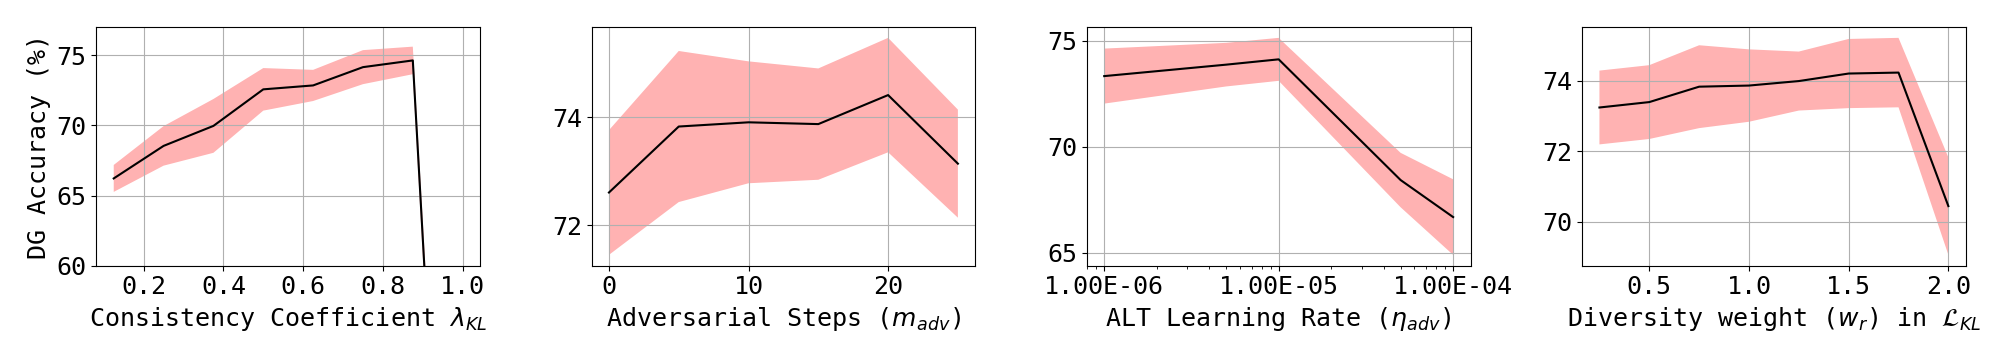
\includegraphics[width=\linewidth]{alt/figures/digits_hyperparam.png}
    \caption{\small{\textbf{Ablation Analysis:} We study the effect of each hyper-parameter in ALT on the average accuracy using the Digits benchmark. For each experiment we show 1 standard deviation around the mean over 5 runs. We observe that the consistency (left most) is generally important until a certain point, after which it becomes harmful; (left center) taking more adversarial steps improves performance; (right center) similarly, a small learning rate is preferred in training the adversary network, $g$, and performance degrades as the learning rate increases; (right most) Surprisingly, we find that the trade-off between diversity and ALT is non- trivial and dataset dependent.}}
    \label{fig:digits_hp}
\end{figure*}

\begin{table*}[t]
    \centering
    % \small
    \resizebox{\linewidth}{!}{
    \begin{tabular}{@{}l ccc ccc ccc ccc c@{}}
        \toprule
        \textbf{Method} & \textbf{A$\rightarrow$C} & \textbf{A$\rightarrow$S} & \textbf{A$\rightarrow$P} & \textbf{C$\rightarrow$A} & \textbf{C$\rightarrow$S} & \textbf{C$\rightarrow$P} & \textbf{S$\rightarrow$A} & \textbf{S$\rightarrow$C} & \textbf{S$\rightarrow$P} & \textbf{P$\rightarrow$A} & \textbf{P$\rightarrow$C} & \textbf{P$\rightarrow$S} & \textbf{Average}\\
        \midrule
        ERM                                 & 62.3 & 49.0 & 95.2 & 65.7 & 60.7 & 83.6 & 28.0 & 54.5 & 35.6 & 64.1 & 23.6 & 29.1 & 54.3\\
        JiGen~\citep{carlucci2019domain}     & 57.0 & 50.0 & 96.1 & 65.3 & 65.9 & 85.5 & 26.6 & 41.1 & 42.8 & 62.4 & 27.2 & 35.5 & 54.6\\
        ADA~\citep{volpi2018generalizing}    & 64.3 & 58.5 & 94.5 & 66.7 & 65.6 & 83.6 & 37.0 & 58.6 & 41.6 & 65.3 & 32.7 & 35.9 & 58.7 \\
        AugMix~\citep{hendrycks2019augmix}   & 68.4 & 54.6 & 95.2 & 74.3 & 66.7 & 87.3 & 40.0 & 57.4 & 46.8 & 67.3 & 26.8 & 41.4 & 59.6 \\
 
        RandConv~\citep{xu2020robust}        & 61.1 & 60.5 & 87.3 & 57.1 & 72.9 & 73.7 & 52.2 & 63.9 & 46.1 & 61.3 & 37.6 & 50.5 & 60.3\\
        SagNet~\citep{nam2021reducing}       & 67.1 & 56.8 & 95.7 & 72.1 & 69.2 & 85.7 & 41.1 & 62.9 & 46.2 & 69.8 & 35.1 & 40.7 & 61.9 \\
        \midrule 
        ALT$_{g-only}$                  & 63.5 & 63.8 &	94.9 & 68.9 & 74.4 & 84.6 & 39.7 & 61.1 & 49.3 &	68.8 & 43.4 & 50.8 & \textbf{63.6}\\
        ALT$_{RandConv}$                    & 63.6 & 65.8 & 92.5 & 69.1 & 75.1 & 84.5 & 40.1 & 61.7 & 50.8 & 68.4 & 43.4 & 55.2 & \textbf{64.2}\\
        ALT$_{AugMix}$                      & 65.7 & 68.2 & 93.2 & 71.9 & 74.2 & 86.0 & 40.2 & 62.9 & 49.1 & 68.5 & 43.5 & 53.3 & \textbf{64.7}\\
        % AugMax                            & 85.4 & 79.6 & 90.1 & 77.1 & 77.4 & 84.3 & 37.0 & 41.9 & 45.9 & 66.8 & 54.6 & 53.5 & 66.1 \\
        \bottomrule 
    \end{tabular}
    }
    \caption[SSDG PACS]{
        Single-source domain generalization accuracy (\%) on PACS~\citep{csurka2017domain}. 
        \textit{X$\rightarrow$Y} implies X is the source dataset and Y is the target dataset.
        \textit{P: photo; A: art-painting; C: cartoon; S: sketch.}
        Performance is reported as mean of 5 repetitions\footnotemark[1].
    }
    \label{tab:results_pacs}
\end{table*}


\subsection{PACS}
\footnotetext{$^*$standard deviation values are in the supplementary material.}
\paragraph{Baselines.}
Our baselines include JiGen~\citep{carlucci2019domain}, adversarial data augmentation (ADA)~\citep{volpi2018generalizing}, AugMix, RandConv, and SagNet~\citep{nam2021reducing} which is designed to reduce style bias using normalization techniques.
We use ResNet18~\citep{he2016deep} pre-trained on ImageNet as our model architecture and train all models for $2000$ iterations with batch-size of $32$, learning rate $0.004$, \texttt{SGD} optimizer with cosine annealing learning rate scheduler, weight decay of $0.0001$, and momentum $0.9$.
For ALT, we set consistency coefficient $\lambda_{KL}{=}0.75$, adversarial learning rate $\eta_{adv}{=}5e{-}5$, number of adversarial steps $m_{adv}{=}10$ and $w_r{=}1.0$.

\paragraph{Results.}
Results are shown in Table~\ref{tab:results_pacs}.
We observe that ALT without a diversity module (ALT$_{g-only}$) surpasses generalization performance of all prior methods including diversity methods RandConv and AugMix and the previous best SagNet~\citep{nam2021reducing}.
ALT with adaptive diversity further improves the results and ALT$_{AugMix}$ establishes a new state-of-the-art accuracy of $64.7\%$.
The most difficult target domains for previous methods has been \textit{Sketch (S)} since this is a set of rough human-drawn black-and-white sketches of real-life objects; the difficluty can be observed in terms of performance in columns $A{\rightarrow}S$, $C{\rightarrow}S$, and $P{\rightarrow}S$.
ALT significantly improves the performance on the sketch target domain, compared to the previous best.
ALT is also the best when generalizing from photos as the source to C,S,A as targets.
This is a very realistic setting since large-scale natural image datasets such as ImageNet~\citep{deng2009imagenet} are widely used and publicly available, while datasets for sketches, cartoons, and painting are not.

\begin{table*}[t]
    \centering
    % \small
    \resizebox{\linewidth}{!}{
    \begin{tabular}{@{}l ccc ccc ccc ccc c@{}}
        \toprule
        \textbf{Method} & \textbf{A$\rightarrow$C} & \textbf{A$\rightarrow$P} & \textbf{A$\rightarrow$R} & \textbf{C$\rightarrow$A} & \textbf{C$\rightarrow$P} & \textbf{C$\rightarrow$R} & \textbf{P$\rightarrow$A} & \textbf{P$\rightarrow$C} & \textbf{P$\rightarrow$R} & \textbf{R$\rightarrow$A} & \textbf{R$\rightarrow$C} & \textbf{R$\rightarrow$P} & \textbf{Average}\\
        \midrule
        ERM                                 & 42.61 & 59.18 & 69.45 & 48.37 & 56.09 & 59.38 & 46.07 & 40.18 & 68.19 & 63.12 & 45.13 & 74.34 & 56.00 \\
        AugMix~\citep{hendrycks2019augmix}   & 45.31 & 61.88 & 71.88 & 49.30 & 58.93 & 62.24 & 50.04 & 42.59 & 71.51 & 64.10 & 47.56 & 75.95 & 58.44 \\
        RandConv~\citep{xu2020robust}    & 43.98 & 55.28 & 67.31 & 45.49 & 56.58 & 59.03 & 43.80 & 43.19 & 66.50 & 57.62 & 48.26 & 72.97 & 55.00\\
        SagNet~\citep{nam2021reducing}   & 42.18 & 56.03 & 67.34 & 46.68 & 53.89 & 57.88 & 45.49 & 40.09 & 67.11 & 61.39 & 48.32 & 72.79 & 54.93\\
        \midrule 
        ALT$_{g-only}$                  & 47.26 & 61.14 & 71.21 & 48.88	& 57.81 & 60.99	& 48.15 & 46.70 & 69.30 & 64.85 & 52.84 & 76.28 & \textbf{58.78} \\
        ALT$_{RandConv}$                & 48.33 & 61.19 & 71.75 & 50.13 & 58.82 & 62.26 & 49.21 & 47.03 & 70.53 & 64.88 & 53.10 & 76.07 & \textbf{59.44}\\
        ALT$_{AugMix}$                  & 48.06 & 61.16 & 71.12 & 50.43 & 58.84 & 61.84 & 49.32 & 47.55 & 70.64 & 64.86 & 53.27 & 76.29 & \textbf{59.45} \\
        \bottomrule 
    \end{tabular}
    }
    \caption[SSDG Office-Home]{Single-source domain generalization accuracy (\%) on Office-Home~\citep{venkateswara2017deep} 
    % with mean and standard deviation 
    over five repetitions. 
    \textit{X$\rightarrow$Y} implies X is the source dataset and Y is the target dataset.
    \textit{R: real; A: art; C: clipart; P: product.}
    Performance is reported as mean of 5 repetitions\footnotemark[1].
    % ; detailed results with standard deviation values are in the supplementary material.
    }
    \label{tab:results_officehome}
\end{table*}
\subsection{Office-Home}
\paragraph{Baselines.}
For PACS, we follow the protocol from the previous state-of-the-art Sagnet~\citep{nam2021reducing} and use ResNet50 as the model architecture.
% and identical training settings and hyperparameters as PACS.
Note that we do not perform any hyperparameter tuning for OfficeHome and directly apply identical training settings and hyperparameters from PACS.

\paragraph{Results.}
Table~\ref{tab:results_officehome} shows the results on Office-Home.
We observe that RandConv (previous best on Digits) and SagNet (previous best on PACS) perform worse than ERM on OfficeHome, while AugMix is better by $2.44\%$.
All three variants of ALT surpass prior results, with ALT$_{AugMix}$ resulting in the best accuracy of $59.45\%$.
The most difficult target domain for previous methods are \textit{Art (A)} and \textit{Clipart (C)}, possibly because both sets have images with white backgrounds, while real world photos (R) and product images are naturally occurring.
ALT improves performance in each case when with A or C as target domain.
An observation similar to PACS can also be made here -- ALT is the best model under the realistic setting of generalizing from widely available real photos (R) to other domains.

\section{Analysis of ALT}
In this section we study the various components of ALT, and provide insights into their impact on generalization. 
\begin{figure*}
    \centering
    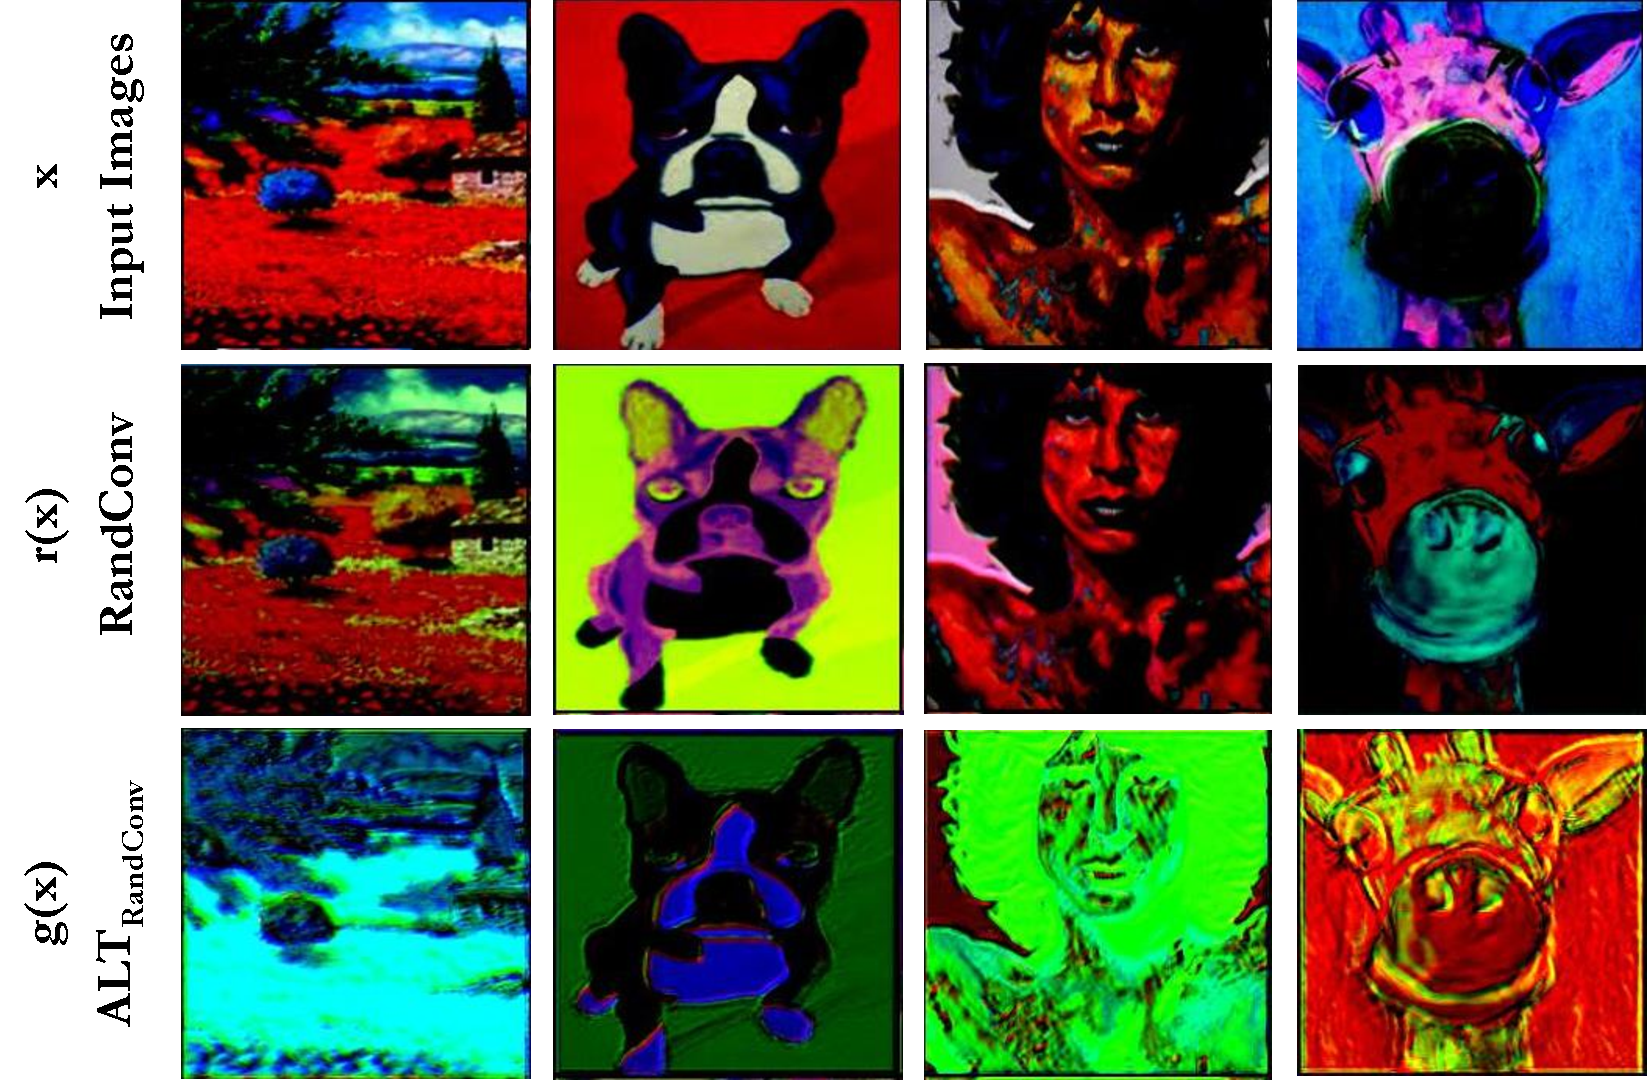
\includegraphics[width=0.48\linewidth]{alt/figures/viz_randconv_alt.pdf}
    \quad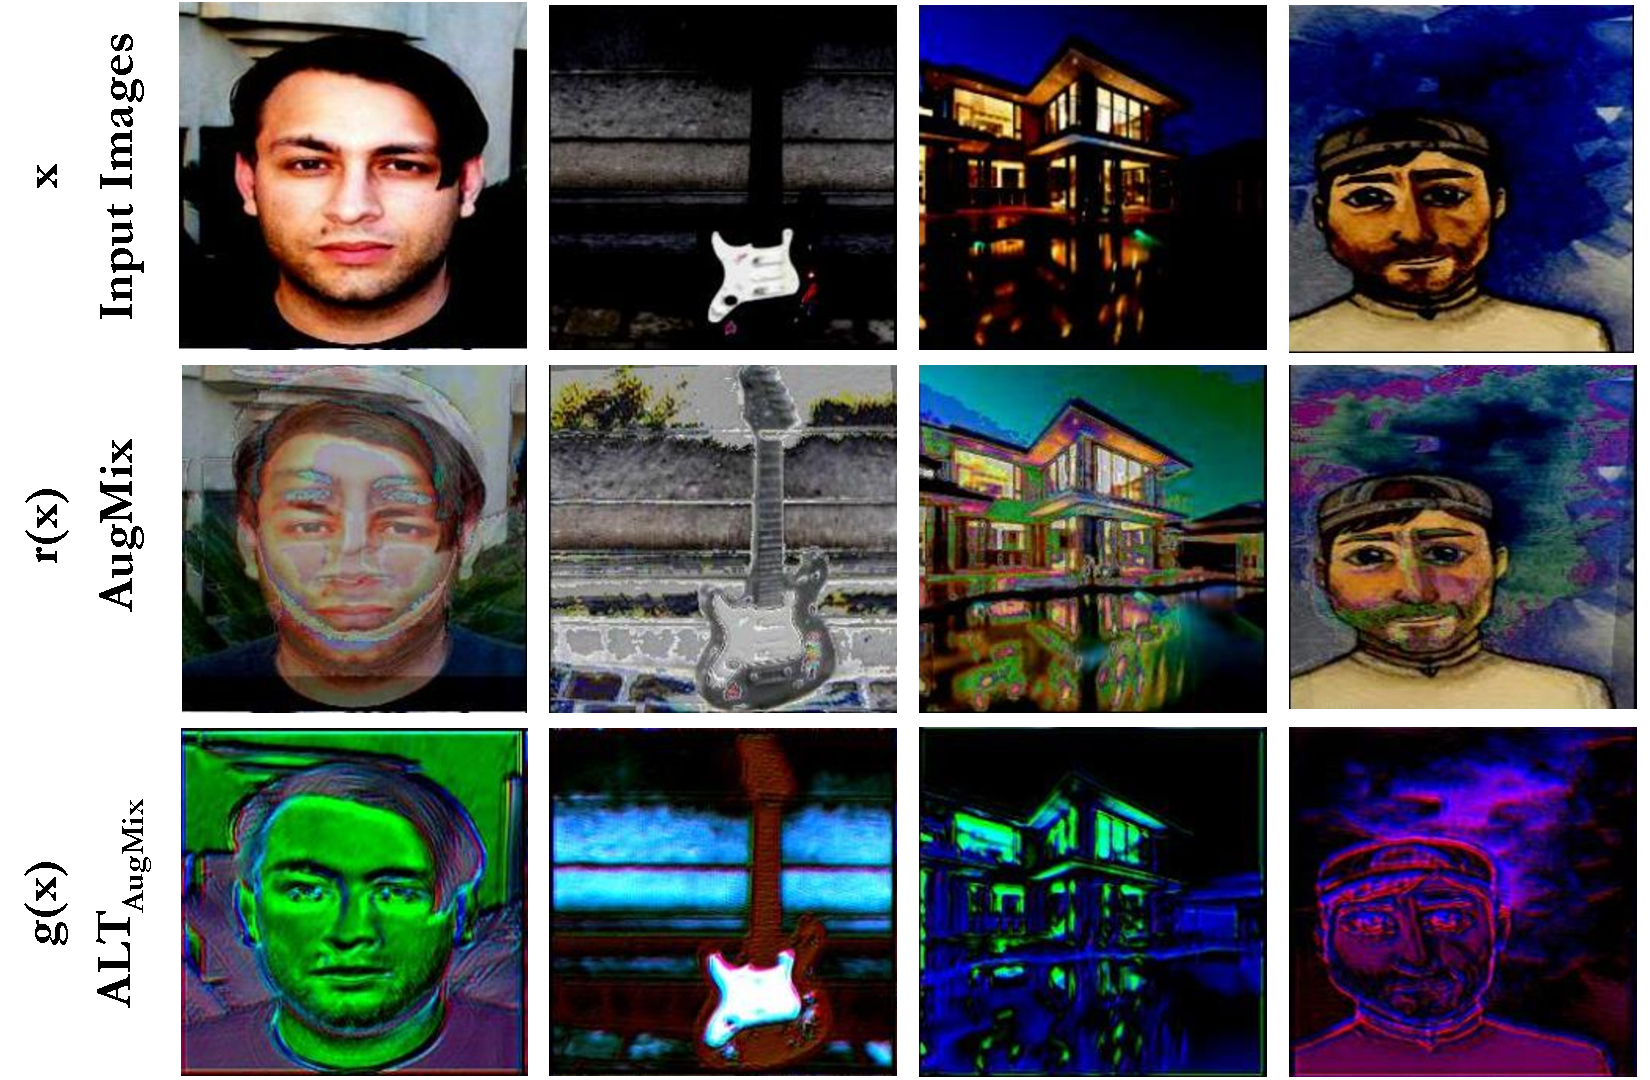
\includegraphics[width=0.48\linewidth]{alt/figures/viz_augmix_alt.pdf}
    \caption{Comparison of images transformed by data augmentation techniques RandConv \textit{(left)} and AugMix \textit{(right)} and their combination with ALT (ALT$_{RandConv}$ and ALT$_{AugMix}$), 
    illustrating the wide range of transformations learned by ALT.}
    \label{fig:viz_augs}
\end{figure*}

\paragraph{ALT is better than na\"ive diversity} Our first big insight is that ALT without an explicit diversity module still outperforms all the top performing methods across the benchmarks we evaluated on, indicating that learned adversarial transformations are a powerful way to train classifiers for generalization. They include diversity (achieved through random initializations) and adversarial images that help expose the classifier to large distribution shifts. Our next observation is that ALT makes the choice of diversity module fairly arbitrary. We see this effect on multiple benchmarks -- for example, on the Digits benchmark shown in  \Cref{tab:results_digits}, AugMix has a relatively poor generalization performance when compared with the baseline ERM whereas ALT$_{Augmix}$ achieves state of the art. This is again seen in the Office-Home benchmark shown in \Cref{tab:results_officehome}, where RandConv is worse than ERM, but ALT$_{RandConv}$ is the best performing method. We show examples of the image transformations learned with ALT in Figure~\ref{fig:viz_augs}, and it is clear that ALT achieves far more diverse and larger transformations of the input images than either AugMix or RandConv.

% - basically talk about diversity alone (Augmix/RC) -- see some boost, but varying results on each benchmark.
% MNIST -- augmix boosts by 1\% barely, but big jump for RandConv.
% On PACS and OfficeHome, AugMix is better than RandConv.
% - ALT without diversity is better than Diversity alone
% - ALT can better adapt its diversity when combined with RandConv and Augmix -- the combination and interplay between the adversarial cost and consistency, is key.


\paragraph{ALT Hyperparameters.}
The four main hyper-parameters that control ALT are: the consistency coefficient $\lambda_{KL}$ in Equation~\ref{alt:eq:L_KL} which decides the proportion between the classifier loss and KL-divergence consistency between transformations, 
number of adversarial steps and learning rate in the adversarial maximization of Equation~\ref{alt:eq:adv_max}, and the diversity weight $w_r$ which controls the interaction between the diversity module $r()$ and the adversary network $g()$ in Equation~\ref{alt:eq:p_mix}.
We investigate the effect of each of these on domain generalization accuracy in Figure~\ref{fig:digits_hp}.
The first plot shows that the consistency coefficient $\lambda_{KL}$ is impactful and a higher value leads to better generalization.
However at $\lambda_{KL}=1.0$ the accuracy degenerates to random performance; this is expected as the classifier loss gets $1-\lambda_{KL}{=}0$ weight.
From the second and third plots, we observe that an optimal value exists around 20 adversarial steps and learning rate of $1e{-}5$.
There is a fast drop in generalization at higher learning rates.
Increasing the diversity weight also leads to increase in generalization, however at $w_r{=}2$ the performance drops and corresponds to "diversity only" settings.
Clearly, the adversarial component is a critical factor that causes improvements in generalization.

\begin{table}[t]
    \centering
    % \small
    \begin{tabular}{@{}lccc@{}}
        \toprule
        \textbf{Architecture} & \textbf{Digits Average} & \textbf{PACS Average} \\
        \midrule
        FCN (2 layers) & 72.75 & 63.40 \\
        FCN (3 layers) & 73.74 & 63.92\\
        FCN (4 layers) & 74.10 & 64.41 \\
        FCN (5 layers) & 73.87 & 64.20 \\
        FCN (6 layers) & 74.15 & 63.78\\
        % ResNetGen-6~\cite{johnson2016perceptual} & \\
        % UNet-10~\cite{ronneberger2015u} & \\
        \bottomrule
    \end{tabular}
    \caption{Effect of the architecture of the adversity network $g$ on average domain generalization on the PACS and Digits benchmarks.}
    \label{tab:gvars}
\end{table}

% \begin{table}[t]
%     \centering
%     \begin{tabular}{cc}
%         \toprule
%         \textbf{Method}     & \textbf{DG Avg.}\\
%         \midrule
%         RandConv            & \\
%         AugMix              & 59.56\\
%         ALT$_{RandConv}$    & \\
%         ALT$_{AugMix}$      & \\
%         ALT$_{none}$        & \\
%         \bottomrule
%     \end{tabular}
%     \caption{PACS DG Average}
%     \label{tab:ablation_hd}
% \end{table}

\paragraph{Complexity of Adversary Network.}
In our experiments on the benchmark datasets we have used a simple fully convolutional network (FCN) with 5 convolutional layers.
We conduct additional analysis to understand how this choice affects generalization performance, and compare performance when using between 2 and 6 convolutional layers.
% We compare FCN with number of layers between 2 and 6.
% and two additional architectures -- U-Net-10~\citep{ronneberger2015u} with 5 downsampling and 5 upsampling operations (UNet-10) and a ResNet based generator (ResNetGen-6) with 3 downsampling and 3 upsampling operations. operations~\citep{johnson2016perceptual}.
% Note that the UNet and ResNet generators are considerably more sophisticated than FCN, and contain bottleneck architectures and skip connections.
We reuse all other training settings from our benchmark model $ALT_{RandConv}$ on both Digits and PACS.
For PACS, we observe that all ALT models compared are better than previous baselines including AugMix and RandConv.
For Digits, we observe that performance of ALT with a 2-layer $g$ is close to RandConv, and is greater than all previous baselines for higher depth of the network.
Increasing the number of layers, i.e., increasing the complexity of the adversary network leads to better performance upto 5 layers, even with the same learning rate.

% \paragraph{Qualitative Comparison of Diverse Augmentations}

% \begin{figure}[t]
%     \centering
%     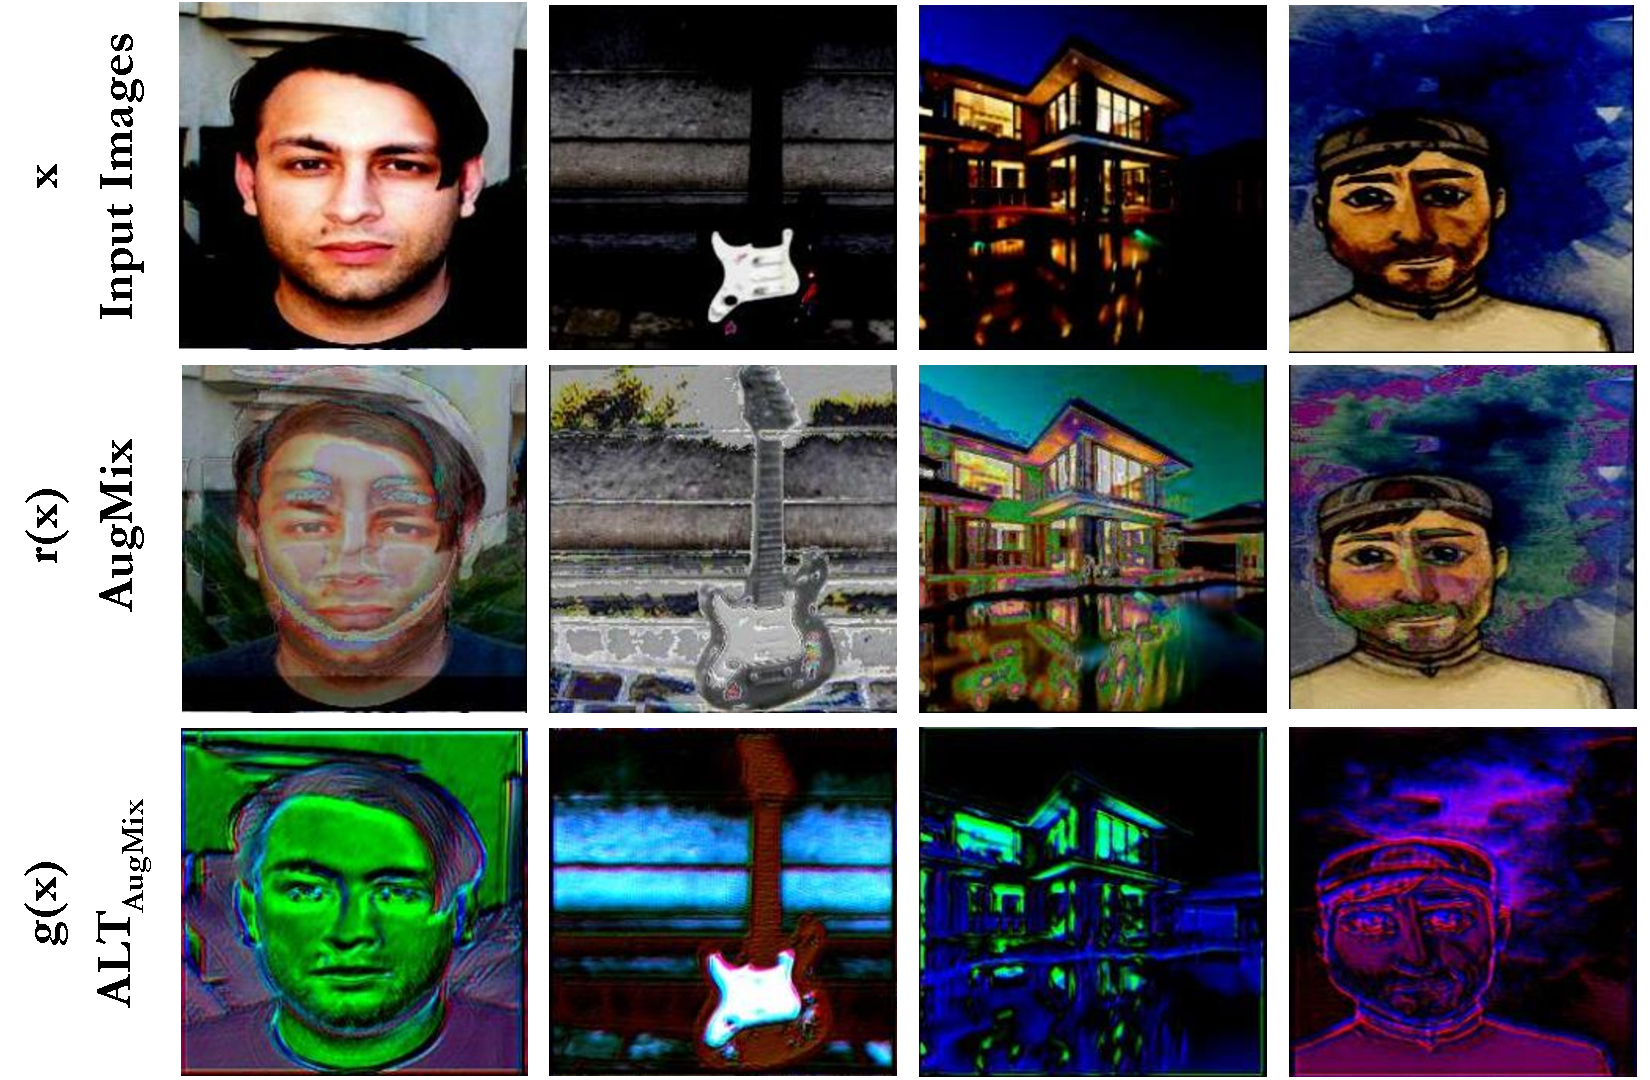
\includegraphics[width=\linewidth]{alt/figures/viz_augmix_alt.pdf}
%     \caption{Comparison of transformed images for AugMix and ALT$_{AugMix}$.}
%     \label{fig:viz_augmix}
% \end{figure}
% In Figure~\ref{fig:viz_augs} we illustrate the difference between the augmentations generated by RandConv, AugMix, ALT$_{g-only}$, ALT$_{RandConv}$ and ALT$_{AugMix}$.


\section{Conclusion}
In this paper, we address the problem of single source domain generalization. Our approach, Adversarially Learned Transformations (ALT) uses a randomly initialized convolutional network to learn plausible image transformations of the source domain that can fool the classifier. These images are used to enforce a consistency with the predictions on clean images. We showed that this strategy outperforms all existing techniques on multiple benchmarks because it is able to generate a diverse set of large transformations of the source domain. 
%
% In this paper, we started with the hypothesis that diversity alone or adversarial training alone is not enough for generalizing to unseen domains in the single-source domain generalization setting, as was confirmed by our experiments and mixed results on prior methods on different benchmarks.
We also find that ALT can be naturally combined with existing diversity modules like RandConv or AugMix to improve their performance (sometimes significantly). We also studied the different parts of ALT through extensive ablations and analysis to obtain insights into its performance gains. Our studies indicate that na\"ive diversity alone is insufficient, but needs to be combined adversarial transformations to maximize generalization performance. 



\chapter{Research Plan}
\label{chap:proposed}
\noindent\textbf{Ph.D. Graduation Estimated Timeline}

\quad\textit{Comprehensive Exam:} Feb 2022

\quad\textit{Proposal Oral:} Mar 2022

\quad\textit{Dissertation Defense:} Feb-Apr 2023\\


\noindent My proposed future work will build on the my work in image classification and V\&L described in the previous chapters by pursuing two key directions:
\begin{itemize}
    \item new algorithms and methods that can improve generalization and robustness of computer vision models, and
    \item analytical and/or theoretical study of the relationship between robustness and domain generalization.
\end{itemize}

\noindent Some of these planned and ongoing projects that are part of this research plan are described below; Table~\ref{tab:research_plan} contains a summary of my contributions.


\section{Empirical Study of Data Modification on Adversarial Robustness}
Generalization and robustness are critical factors that affect the reliability of machine learning models. 
In NLP and vision literature, methods designed for domain generalization report performance on relevant \textit{IID} and \textit{OOD} test sets, but the effect of these methods on adversarial robustness remains unmeasured.
Since methods designed for out-of-domain \textit{(OOD)} generalization are usually a combination of additional training data and new architectures and optimization techniques, we would like to evaluate common categories of methods: training with additional datasets, data augmentation, model debiasing, and data filtering, in comparison with each other.
In this project, we start with identifying five key categories of methods developed for the purpose of increasing out-of-domain generalization or used as baselines.
Our plan is to study the performance of these methods on tasks such as image classification which have standard benchmarks for both OOD generalization as well as adversarial robustness.
Our aim is to understand whether the increase or decrease in OOD generalization by each method over the naive baseline is consistent across tasks.
To further conduct fine-grained analysis, we will also analyze the effect of these methods on in-domain (IID) accuracy on the test set for each task, since in the ideal case improvement in OOD performance should not come at the cost of in-domain accuracy.
Our next aim is to understand the effect of these generalization methods on adversarial robustness.
The results of a synthetic bianry classification task where points lie in a 2-dimensional feature space and separated by concentric circles into class labels.
This setting allows us to visualize the effect of various techniques that alter the training data such as using multiple datasets, automated data augmentation, and algorithmic data filtering, on the training distribution and the resulting performance.
\begin{figure}
    \centering
    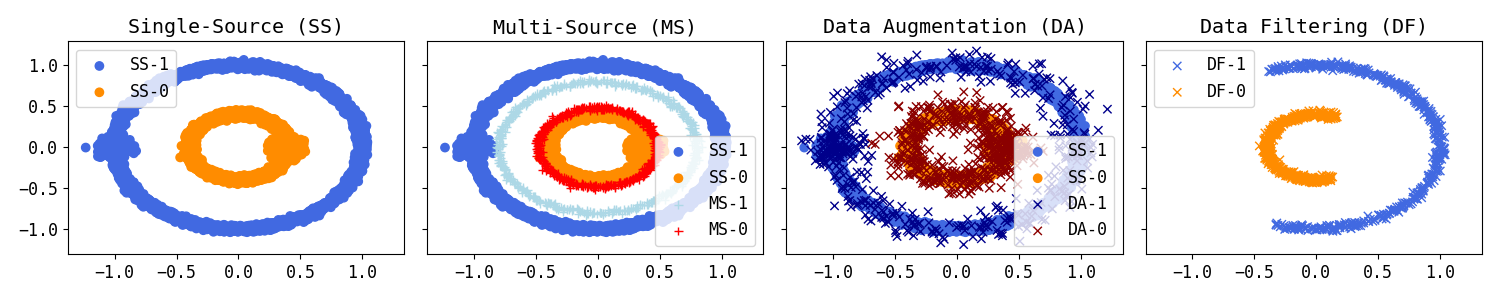
\includegraphics[width=\linewidth]{figures/viz_effect_on_distrib.png}
    \caption{Our toy experimental setting consists of points in $\R^2$ belonging to two classes (0/1).
    This illustration shows the discrepancy between the source dataset (\texttt{SS}) and the out-of-domain dataset (\texttt{OOD}).
    }
    \label{fig:viz_effect_on_distrib}
\end{figure}
% Recent work seeks to understand the relationships between in-domain and out-of-domain performance: for instance,~\citet{miller2021accuracy} empirically show that IID and OOD performance are strongly correlated,~\citet{raghunathan2020understanding,yang2020closer} focus on understanding the tradeoff between robustness and accuracy for adversarially trained models.
% However it is not clear how methods \textit{designed for generalization} affect robustness.
% This is largely because work on domain generalization reports only IID and OOD metrics, and work on robustness reports only IID and robustness metrics.
% This paper seeks to evaluate for the first time, the effect of models designed specifically for generalization on adversarial robustness.
% Our findings can be summarized as follows:
% \begin{itemize}[noitemsep,nosep]
%     \item More data benefits OOD generalization, 
%     \item Data filtering hurts OOD generalization, and
%     \item Data filtering significantly hurts adversarial robustness on all benchmarks.
% \end{itemize}
% % \TG{the sentences that follow can fit well either here or in the conclusion -- decide who to split / tone.}
% These findings and our additional analysis raise new questions for robustness and domain generalization research.
% Significant among these are the importance of both diversity and number of training samples for inductive bias and generalization guarantees, the problems associated with data filtering in terms of robustness, and the importance of a comprehensive set of evaluation metrics that could be adopted for future work.
% In this proposed project, we plan to conduct a comprehensive study of these categories
% on three tasks -- natural language inference (NLI), question answering (QA), and image classification (IC), and evaluate them not only on IID and OOD accuracies, but also on their adversarial robustness (AR).
% We also present results and visualizations on a 2-dimensional synthetic dataset in order to gain grounded insights about the effects of each method on the training distribution.
% Our findings suggest that more data (either via additional datasets or data augmentation) benefits both OOD and AR.
% On the other hand, we find that data filtering (known to improve OOD accuracy on NLI) hurts OOD accuracy on QA and IC, and hurts robustness on all three tasks.

\section{Interpolation as an Analysis Tool for Studying Robustness and Generalization}
We plan to use interpolation between samples from source and target domain in order to understand and characterize model behavior, and obtain a metric for domain shift as a function of this model behavior.

Consider a classification task with label set $\mathcal{Y}$.
For this task, let $\mathcal{X}^{id}$ be the domain from which training images are samples (\textit{id} stands for in-domain).
Let $\mathcal{X}^{od}$ be the domain of images that are out-of-distribution and unseen during training.
In general, $\mathcal{X}^{od}$ can be made of several distinct domains $\mathcal{X}^{od}_1 \dots \mathcal{X}^{od}_{D}$, but we will denote all of them together as  $\mathcal{X}^{od}$ for brevity.
To ground this, we shall use the example of the PACS benchmark where the label set is $\mathcal{Y} = \{ \textrm{`dog' `elephant', `horse', `person', `giraffe', `house', `guitar'}\}$, $\mathcal{X}^{id}$ is a set of photographs, while the $\mathcal{X}^{od}$ is made up of images belong to the same classes, but art/painting, cartoons, and sketches (instead of photographs).

\begin{wrapfigure}{r}{0.5\linewidth}
    \centering 
    \includegraphics[width=0.6\linewidth]{figures/patch_grid_horse.pdf}
    \caption{Illustration of the division of an image into patches.}
    \label{fig:patch_grid_horse}
\end{wrapfigure}
Now consider a set of classifier models trained on $X_{id}$ until convergence, $\mathcal{F} = \{f_1, \dots, f_K\}$.
We wish to divide each image into a set of non-overlapping patches.
Let this number of patches belong to the set $\mathcal{P}=\{p_1, \dots, p_N\}$.
Given any two images $x_1, x_2$, we interpolate between these two images by randomly selecting one of the $p$ patches from both images and swapping them.
We repeat this process until all patches from image $x_1$ have been replaced by the corresponding patches from $x_2$.
Thus, for $p$ patches, our interpolation method requires $p$ steps of patch-swapping.
At each step $t$, we obtain a resulting \textit{interpolated} image $x_{in}^t (p)$ and for each model $f$, we can obtain class-predictions $y_{in}^t (f, p)$ for these interpolated images.
This intuitive process is explained mathematically in Algorithm~\ref{algo:patchwise_interpolation}.

Thus for each pair of samples $x_1$, $x_2$ we get a sequence of interpolated images and their predictions $X_{x_1, x_2}(p)$ and $Y_{x_1, x_2}(f, p)$ respectively.
From $Y$, we can compute the number of transitions between subsequent predictions -- this measures how frequently the predictions fluctuate from one class label to another during the process of interpolation.
This quantity, $z$, gives us a measure of how sensitive the model $f$ is to interpolations using $p$ patches.
(Note: larger $p$ implies smaller patch size).
Thus we name this quantity \textit{``interpolation sensitivity"} and compute it as:
\begin{equation}
    z_{x_1, x_2} (f, p) = \frac{1}{p}\sum_{i=1}^{p}\mathbbm{1}\Big( Y_{x_1, x_2}(f, p)[i] == Y_{x_1, x_2}(f, p)[i-1]\Big)
\end{equation}

\begin{algorithm}
    \caption{PATCHWISE INTERPOLATION for images}
    \begin{algorithmic}[0]
        \State \textbf{Input:} images $x_1$, $x_2$, model $f$, number of patches $p$
        \State \textbf{Output:} interpolated image sequence $X_{x_1, x_2}(p)$ and output sequence $Y_{x_1, x_2}(f, p)$
    \end{algorithmic}
    \begin{algorithmic}[1]
        \State \textbf{Initialize:} $M = \underline{\mathbf{0}}^{H\times W}$ \algorithmiccomment{\textit{initialize mask as a matrix of all zeros}}
        \ForEach{$t \in \{1\dots p\}$}%
            \State $q \widesim[3]{w/o~repl.} \{1, \dots, p\}$ \algorithmiccomment{\textit{sample patch index without replacement}}
            \State $M[q] \gets 1$ \algorithmiccomment{\textit{set patch $q$ elements to 1}}
            \State $x_{in}^t (p) \gets x_1\odot (1-M) + x_2\odot M$ \algorithmiccomment{\textit{interpolate}}
            \State $y_{in}^t (f, p) \gets f(x_{in}^t (p) $ \algorithmiccomment{\textit{get predicted class}}
        \EndForEach
        \State $X_{x_1, x_2} (p) \gets [x_{in}^1(p) \dots x_{in}^p(p)]^T$
        \State $Y_{x_1, x_2} (f, p) \gets [y_{in}^1(f,p) \dots y_{in}^p(f,p)]^T$
        \State\Return $\theta$
\end{algorithmic}
\label{algo:patchwise_interpolation}
\end{algorithm}



Given this formula for computing pairwise interpolation sensitivity, we can also compute a dataset-level statistic, depending on the domain of $x_1$ and $x_2$.
\begin{align}
    Z^{id-id} (f, p) &= \underset{x_1, x_2 \in \mathcal{X}^{id}}{\E} z_{x_1, x_2}(f, p) \\
    Z^{od-od} (f, p) &= \underset{x_1, x_2 \in \mathcal{X}^{od}}{\E} z_{x_1, x_2}(f, p) \\
    Z^{id-od} (f, p) &= \underset{\substack{x_1 \in \mathcal{X}^{id},\\ x_2\in\mathcal{X}^{od}}}{\E} \frac{1}{2}(z_{x_1, x_2}(f, p) + z_{x_2, x_1}(f, p))
    \label{eq:expected_sensitivity}
\end{align}

Armed with this measure of sensitivity, we can now analyse the correlation between out-of-domain accuracy and interpolation sensitivity.
% Let $\mathfrak{Z}$ denote the $|\mathcal{F}|\times|\mathcal{P}|$ matrix where each elemnt $\mathfrak{Z}[i, j]$ represents the sensitivity of model $f_i$ when interpolating with $p_j$ patches.
Let $\mathbb{A}$ be a $K\times 1$ vector of OOD accuracies of each model.
Then we can compute the Pearson correlation of OOD accuracies with sensitivity values at all values of $p$, as:
\begin{align}
    \rho(p)^{id-id} &= corr(\mathbb{A}, [Z^{id-id}(f_1, p), \dots, Z^{id-id}(f_K, p)])\\
    \rho(p)^{id-id} &= corr(\mathbb{A}, [Z^{od-od}(f_1, p), \dots, Z^{od-od}(f_K, p)])\\
    \rho(p)^{id-id} &= corr(\mathbb{A}, [Z^{id-od}(f_1, p), \dots, Z^{id-od}(f_K, p)])
    \label{eq:correlation}
\end{align}

We plan to develop the above and other analytical measures to understand model behavior and connections with adversarial robustness, corruption robustness, and domain shift.
Our hypothesis is that sensitivity values obtained from patchwise interpolations as defined in Algorithm~\ref{algo:patchwise_interpolation} are indicative of model robustness.
While this study will be largely analytical in nature, theoretical connections between domain shift and robustness may emerge, which would be useful for future research on generalization.


\section{Evaluating Robustness of V\&L Systems}
I am leading a project which aims to analyze the relative contributions of visual and textual inputs in multi-modal tasks by analyzing existing models for captioning, question-answering, and reasoning, through the analytical lens of image generation.
The joint study of text-to-image (T2I) and downstream V\&L tasks can enable us to reason both about the quality of existing image synthesis approaches as well as models trained for tasks such as visual question answering, image captioning, retrieval, etc.
I am currently working on preliminary experiments for this project.

In Summer 2022, I will collaborate with researchers at Microsoft Research -- the aim of this project is closely aligned with my thesis topic of studying robust visual understanding.
We are currently in the brainstorming stage for this project.
% I will investigate how sensitive models are to very small perturbations of object locations, and what are the failure modes of these models when it comes to such ``spatial robustness''.

Table~\ref{tab:research_plan} provides a summary of my publications during my Ph.D. as well as a timeline for planned projects.

% \paragraph{Summary of Contributions}


\begin{table}
    \centering
    % \small
    \resizebox{\linewidth}{!}{
    \begin{tabular}{@{}p{0.48\linewidth}clcl@{}}
        \toprule
        \textbf{Short Title} & \textbf{Lead} & \textbf{Venue} & \textbf{Domain} & \textbf{Task}\\
        \midrule
        Visual Planning~\citep{gokhale2019blocksworld}      & $\checkmark$  & $^W$CVPR-19   & V     & Planning \\
         \textbf{VQA-LOL}~\citep{gokhale2020vqa}            & $\checkmark$  & ECCV-20       & V{+}L & VQA\\
        Video2Commonsense~\citep{fang2020video2commonsense} & $\checkmark$  & EMNLP-20      & V{+}L & Captioning, VQA\\
        \textbf{Mutant}~\citep{gokhale2020mutant}           & $\checkmark$  & EMNLP-20      & V{+}L & VQA\\
        \textbf{AGAT}~\citep{gokhale2020attribute}          & $\checkmark$  & AAAI-21       & V     & Img. Cls. \\
        TTL-RC~\citep{banerjee-etal-2021-self}              &               & NAACL-21      & L     & QA \\
        Halluci-Net~\citep{kulkarni2020halluci}             &               & $^W$CVPR-21   & V     & Image Synthesis \\
        \textbf{WeaQA}~\citep{banerjee2021weaqa}            &               & ACL-21 Findings   & V{+}L & VQA \\ 
        \textbf{SpatialVQA}~\citep{banerjee2021weakly}      &               & ICCV-21       & V{+}L & VQA \\
        \midrule 
        \textbf{SDRO}~\citep{gokhale2021semantically}       & $\checkmark$  & (R) ACL-22    & V{+}L & V\&L Inference \\
        PHL Triplet NLI~\citep{varshney2021unsupervised}&              & (R) ACL-22    & L     & NLI \\
        Poly-DPR~\citep{luo2022improving}                   &               & (R) AAAI-22   & L     & Retrieval \\
        \textbf{ALT}                                        & $\checkmark$  & (R) CVPR-22   & V     & Img. Cls. \\
        \midrule 
        \textbf{Effect of Dataset Modification}~\citep{}    & $\checkmark$  & (R) ACL-22    & V, L  & evaluation \\
        \textbf{Robustness Study via Interpolation}         & $\checkmark$  & (P) NeurIPS-22 & V{+}L & evaluation \\
        \textbf{Unsupervised Spatial VQA}                   & $\checkmark$  & (P) NeurIPS-22 & V{+}L & VQA \\      
        \textbf{Joint Evaluation T2I and V\&L}              & $\checkmark$  & (P) EMNLP-22  & V{+}L & evaluation \\
        \textbf{V\&L Pre-Trained Model Robustness} (with MSR, Summer 2022) & $\checkmark$ & 2023 & V{+}L \\
        \bottomrule
    \end{tabular}
    }
    \caption{
    Chronological publications and future research plan.
    Abbreviations: \textit{$^W$: Workshop proceedings, $\checkmark$: main author, (R): under review, (P): planned submission, V: vision, L: language, \textbf{bold}: described in this proposal
    }
    }
    \label{tab:research_plan}
\end{table}


\clearpage
%-----------------------back matter
{\singlespace
% Making the references a "part" rather than a chapter gets it indented at
% level -1 according to the chart: top of page 4 of the document at
% ftp://tug.ctan.org/pub/tex-archive/macros/latex/contrib/tocloft/tocloft.pdf
\addcontentsline{toc}{part}{REFERENCES}
\bibliographystyle{asudis}
\bibliography{bibs/tgokhale} %,bibs/bib_agat,bibs/bib_vqalol,bibs/bib_sdro,bibs/bib_alt}

% \appendix
% \renewcommand{\chaptername}{APPENDIX}
% \addtocontents{toc}{RESEARCH PLAN \par}
% \include{vita}
\addcontentsline{toc}{part}{BIOGRAPHICAL SKETCH}
\newpage
\biographicalpage{\\Enter content here.}
% \chapter{Biography}
% Tejas Gokhale was born and raised in Maharashtra, India.
% He is a native speaker of Marathi, Hindi, and English; can read, write, and speak Urdu; understand basic Sanskrit, Punjabi, Gujarati, Konkani, and Spanish; and is trying to learn Putonghua.
% He received his bachelor's degree from Birla Institute of Technology and Science, spent two wonderful years in at Carnegie Mellon University in Pittsburgh PA, where he received a Master of Science degree in Electrical and Computer Engineering, and the last four years in Tempe AZ for his PhD.
% Tejas has worked as an intern at ST Microelectronics, Snap, and Lawrence Livermore National Laboratory.
\end{document}
